\documentclass[lang=cn,10pt,chinese]{elegantbook}

\title{微分几何与广义相对论}

\author{真田信繁}
\institute{Your Institute}
\date{\today}
\bioinfo{主题}{微分几何与广义相对论}

\extrainfo{从流形到爱因斯坦场方程}

\setcounter{tocdepth}{3}

% 额外的宏包
\usepackage{tikz}
\usetikzlibrary{arrows.meta,decorations.pathmorphing,backgrounds,positioning,calc,3d,patterns}
\usepackage{subcaption}
\usepackage{physics}
\usepackage{braket}
\usepackage{cancel}
\tikzset{every picture/.style={line width=0.75pt}}

% 参考文献资源 (elegantbook.cls 自动加载 reference.bib)
\ExecuteBibliographyOptions{sorting=none}

% 自定义命令
\newcommand{\M}{\mathcal{M}}           % 流形
\newcommand{\T}{\mathcal{T}}           % 切丛
\newcommand{\Tstar}{\mathcal{T}^*}     % 余切丛
\newcommand{\Lag}{\mathcal{L}}         % 拉格朗日量
\newcommand{\Ham}{\mathcal{H}}         % 哈密顿量
\newcommand{\Riem}{\mathrm{Riem}}      % 黎曼曲率张量
\newcommand{\Ric}{\mathrm{Ric}}        % 里奇张量
\newcommand{\Rcal}{R}                  % 标量曲率
\newcommand{\g}{\mathrm{g}}            % 度规
% \dd is already defined by physics package
\newcommand{\pd}{\partial}             % 偏导数
\newcommand{\Lie}{\mathcal{L}}         % 李导数
\newcommand{\diag}{\operatorname{diag}} % 对角矩阵
\newcommand{\Order}{\mathcal{O}}       % 量级符号

\begin{document}

\maketitle
\frontmatter

\tableofcontents

\mainmatter
%=============================================================================
% 第一部分：微分几何基础
%=============================================================================

% chapter01.tex - 引言
\chapter{引言 (Introduction)}

\section{微分几何与物理学的关系}

微分几何是数学中研究光滑流形上的几何结构的分支，它为现代物理学提供了不可或缺的语言和工具。从牛顿力学到爱因斯坦的广义相对论，从麦克斯韦电磁理论到杨--米尔斯规范场论，物理学家发现了一个深层的真理：\textbf{自然界的定律本质上是几何的}。

\begin{note}[物理动机]
为什么物理学需要微分几何？答案在于一个看似平凡却极其深刻的原理：物理定律应当与坐标系的选择无关——这就是\textbf{广义协变性原理}。当我们选择不同的坐标系来描述同一个物理系统时，物理定律的形式必须保持不变。微分几何恰好提供了描述这种与坐标无关的几何结构的完整数学工具。
\end{note}

要理解这一思想的核心，我们可以从一个简单的问题出发：什么是"直线"？在欧几里得空间中，我们自然地回答"两点之间最短的路径"。但在弯曲的曲面上——比如球面——这个简单的概念需要重新审视。球面上两点之间的最短路径是连接它们的大圆弧，而非嵌入空间中的"笔直"线段。这个简单的观察揭示了一个关键事实：\textbf{几何结构决定了物体如何在空间中运动}。

\begin{figure}[htbp]
\centering
\begin{tikzpicture}[scale=1.3]
    % 球面
    \shade[ball color=blue!15,opacity=0.6] (0,0) circle (1.8);
    \draw (0,0) circle (1.8);
    % 赤道大圆
    \draw[red,thick] (-1.8,0) arc (180:360:1.8 and 0.5);
    \draw[red,thick,dashed] (-1.8,0) arc (180:0:1.8 and 0.5);
    % 两个点
    \fill[red] (-1.2,0.7) circle (0.06) node[above left] {$p$};
    \fill[red] (1.2,-0.5) circle (0.06) node[below right] {$q$};
    % 大圆弧
    \draw[red,thick] (-1.2,0.7) .. controls (-0.5,1.3) and (0.5,-0.1) .. (1.2,-0.5);
    \node[red] at (0.1,0.9) {测地线（大圆）};
    % 标注
    \node at (-2.0,-1.3) {球面 $S^2$};
\end{tikzpicture}
\caption{球面上两点 $p$ 和 $q$ 之间的最短路径是连接它们的大圆弧（测地线），而非三维嵌入空间中的"直线"。在弯曲空间中，几何结构决定了什么是"直的"。}
\label{fig:sphere_geodesic}
\end{figure}

在牛顿力学中，引力被看作一种"力"，它以超距作用的方式吸引物体。但这一描述有一个根本性的问题：为什么\textbf{引力质量} $m_G$（出现在万有引力定律 $F = G M m_G / r^2$ 中）恰好等于\textbf{惯性质量} $m_I$（出现在牛顿第二定律 $F = m_I a$ 中）？牛顿力学对此没有解释，它只能将此视为一个巧合。事实上，现代 E\"ot-Wash 实验已经以 $10^{-15}$ 的相对精度验证了 $m_G = m_I$ —— 这是物理学中最精确验证的等价性之一。

\medskip

\textbf{从 $m_G=m_I$ 到时空弯曲的逻辑链。} 这一等价性的深远意义可以通过以下推理来理解：
\begin{enumerate}
    \item 由于 $m_G=m_I$，所有物体在引力场中以相同的加速度下落——无论其质量或组成如何。
    \item 因此，一个自由下落的观察者无法通过任何局部实验来探测引力场——引力在局部上可以被"变换掉"。
    \item 这意味着引力不是一种普通的力，而是时空本身的结构属性。任何试图将引力纳入平坦时空的努力都会与等效原理相矛盾。
    \item 时空必须被赋予弯曲的几何结构，使得自由粒子沿测地线运动，而这一运动的表观加速度恰好解释了"引力"现象。
\end{enumerate}
这一逻辑链——从 $m_G=m_I$ 出发，经过局部不可分辨性，最终导出时空弯曲——是广义相对论最深刻的思想主线，也是为什么微分几何作为描述弯曲空间的数学语言成为理论物理学的核心工具。

\medskip

爱因斯坦给出了这一"巧合"的深层次解释：\textbf{引力不是一种力，而是时空弯曲的表现}。在弯曲的时空中，自由下落的物体沿测地线——即弯曲时空中对应的"直线"——运动。这一革命性的观念构成了广义相对论的基础，而描述弯曲时空的数学语言正是微分几何。

\medskip

这里值得一提的是\textbf{马赫原理 (Mach's Principle)}。马赫认为，物体的惯性并非其内禀属性，而是由宇宙中所有其他物质共同决定的——一个孤立粒子在空无一物的宇宙中将没有惯性。虽然爱因斯坦深受这一思想的启发，并希望在广义相对论中实现它，但最终的场方程并未完全体现马赫原理（例如，存在非马赫型的德西特宇宙解）。然而，广义相对论确实部分体现了马赫的精神：物质的分布（通过 $T_{\mu\nu}$）决定了时空的几何（通过 $g_{\mu\nu}$），而时空几何又决定了物体的惯性运动。这一物质-几何的相互决定关系成为相对论宇宙学的核心主题，至今仍然活跃在量子引力研究的前沿。

\begin{note}[物理意义：引力的几何本质]
爱因斯坦的洞见可以总结为"引力即几何"。这改变了我们对宇宙的根本理解：
\begin{itemize}
    \item 引力场 = 时空曲率（度规张量 $g_{\mu\nu}$ 描述）
    \item 自由落体 = 沿测地线运动（弯曲时空的"直线"）
    \item 潮汐力 = 相邻测地线的相对加速度（由曲率张量描述）
\end{itemize}
这一框架将引力从一种神秘的"力"转化为可精确计算的几何效应。
\end{note}

\section{历史发展}

微分几何与广义相对论的发展史是一个数学与物理学相互促进的经典案例。

\begin{figure}[htbp]
\centering
\begin{tikzpicture}[
    scale=0.85,
    timeline/.style={->,thick,blue!60},
    event/.style={fill=blue!50,text=white,rounded corners=3pt,inner sep=3pt,font=\small,align=center},
    math_event/.style={fill=green!50!black,text=white,rounded corners=3pt,inner sep=3pt,font=\small,align=center},
    phys_event/.style={fill=red!50,text=white,rounded corners=3pt,inner sep=3pt,font=\small,align=center}
]
    % Time axis
    \draw[timeline] (0,0) -- (16,0) node[right] {时间};
    
    % Gauss 1827
    \draw (0.5,0.3) -- (0.5,-1.5);
    \node[event] at (0.5,-1.8) {Gauss 1827\\Theorema Egregium};
    \node at (0.5,0.6) {1827};
    
    % Riemann 1854
    \draw (3,0.3) -- (3,-1.5);
    \node[event] at (3,-1.8) {Riemann 1854\\$n$维弯曲空间};
    \node at (3,0.6) {1854};
    
    % Ricci & Levi-Civita 1900
    \draw (8,0.3) -- (8,-1.5);
    \node[event] at (8,-1.8) {Ricci \& Levi-Civita 1900\\张量分析（绝对微分学）};
    \node at (8,0.6) {1900};
    
    % Grossmann + Einstein 1913
    \draw (12.5,0.3) -- (12.5,-1.5);
    \node[event] at (12.5,-1.8) {Einstein \& Grossmann\\1913 黎曼几何+物理};
    \node at (12.5,0.6) {1913};
    
    % Einstein 1915
    \draw (15,1.8) -- (15,-0.2);
    \node[event] at (15,2.2) {Einstein 1915\\$G_{\mu\nu}=8\pi G T_{\mu\nu}$};
    \node at (15,1.7) {1915};
    
    % Schwarzschild 1916
    \draw (15,-0.8) -- (15,-2.2);
    \node[event] at (15,-2.5) {Schwarzschild 1916\\第一个黑洞解};
    
    % Weyl, Cartan
    \draw (13.5,-3.2) node[event] {Weyl \& Cartan\\纤维丛与联络};
    
    % Wheeler 1967
    \draw (10,-3.2) node[event] {Wheeler 1967\\"黑洞"命名};
    
    % Penrose & Hawking
    \draw (5.5,-3.2) node[event] {Penrose \& Hawking\\1965-70 奇点定理};
    
    % LIGO 2015
    \draw (1,-3.2) node[event] {LIGO 2015\\引力波探测};
    
    % Labels
    \node[font=\footnotesize\itshape,gray] at (15.5,-3.7) {... 至今};
\end{tikzpicture}
\caption{微分几何与广义相对论的发展简史。绿色代表数学进展，红色代表物理进展。两者相互促进：黎曼几何为广义相对论提供了数学工具，而广义相对论反过来又刺激了现代微分几何的发展。}
\label{fig:history_timeline}
\end{figure}

下面我们对各个关键里程碑进行更详细的叙述。

\begin{enumerate}
    \item \textbf{高斯 (Gauss, 1827) —— 曲面的内蕴几何}：高斯在研究二维曲面时提出了一个划时代的观点：曲面的几何性质可以由曲面自身上的测量来决定，而不需要参考其嵌入的高维空间。他在《关于曲面的一般研究》中证明的 \textbf{Theorema Egregium}（绝妙定理）表明，高斯曲率 $K$ 完全由曲面上的度规系数 $g_{ij}$ 及其偏导数决定，是一个内蕴量。这意味着生活在曲面上的"二维生物"可以通过测量三角形的内角和来探测曲面的弯曲，而无需知晓第三维的存在——这蕴含了现代物理学中"生活在时空中而不需要外部参考"的思想 \cite{Carroll1997}。
    
    \item \textbf{黎曼 (Riemann, 1854) —— 高维黎曼几何}：黎曼将高斯的思想推广到任意维数。在他著名的就职演讲《论作为几何学基础的假设》中，黎曼定义了 $n$ 维弯曲空间的度规：
    \begin{equation}
        \dd s^2 = g_{\mu\nu}(x) \dd x^\mu \dd x^\nu,
    \end{equation}
    并提出曲率完全由度规张量 $g_{\mu\nu}$ 及其导数决定。这一工作为后来爱因斯坦的广义相对论提供了必需的数学框架。
    
    \item \textbf{黎曼曲率张量的发现}：黎曼定义了四阶曲率张量 $R^\lambda{}_{\mu\nu\rho}$，其物理意义是：当一个向量沿无限小闭合回路平行移动一周后，它不回初始方向的偏离量。这正是引力的几何诠释的核心——\textbf{曲率就是引力场}。曲率非零意味着存在潮汐力。
    
    \item \textbf{里奇 (Ricci-Curbastro) 与列维--奇维塔 (Levi-Civita, 1900) —— 张量分析}：里奇和列维--奇维塔发展了所谓的"绝对微分学"（即今天所称的张量分析），将黎曼几何的数学语言系统化为便于物理应用的形式。列维--奇维塔引入了\textbf{平行移动}（parallel transport）的概念，为弯曲空间中的"方向比较"提供了数学基础。他还提出引力的标量理论候选者应该是黎曼标量曲率 $R$——这一步虽然不完整，但为后来爱因斯坦的工作指明了方向 \cite{Wald1984}。
    
    \item \textbf{爱因斯坦与格罗斯曼 (Einstein \& Grossmann, 1912--1915) —— 寻找场方程}：1912 年，爱因斯坦从布拉格返回苏黎世，找到了他的老友马塞尔·格罗斯曼——苏黎世联邦理工学院的数学教授。据说爱因斯坦对他说的第一句话是："格罗斯曼，你必须帮助我，否则我会发疯！" \cite{Wald2019}。格罗斯曼查阅了图书馆的数学文献，发现了黎曼、里奇和列维--奇维塔的工作，意识到这正是描述弯曲时空所需的数学工具。1913 年，两人合作发表了《广义相对论和引力理论纲要》，虽然其中的场方程还不完整，但它已经将物理（等效原理和广义协变性）与数学（黎曼几何）紧密地联系在了一起 \cite{Tong_GR_LectureNotes}。
    
    \item \textbf{爱因斯坦 (1915) —— 场方程的最终形式}：经过两年的艰苦努力，爱因斯坦于 1915 年 11 月在普鲁士科学院连续四周提交了四篇论文，最终完成了场方程的正确形式：
    \begin{equation}
        R_{\mu\nu} - \frac{1}{2}R g_{\mu\nu} = \frac{8\pi G}{c^4} T_{\mu\nu},
    \end{equation}
    并在此框架下解释了水星近日点的反常进动（每世纪 43 角秒，此前是经典力学无法解释的谜题），成功地预言了光线在太阳引力场中的偏折（1919 年日食观测证实，使爱因斯坦一夜之间成为世界名人）。爱因斯坦场方程简洁而深刻：\textbf{左侧是时空几何（爱因斯坦张量），右侧是物质分布（能量-动量张量）}。
    
    \item \textbf{施瓦西 (Schwarzschild, 1916) —— 第一个精确解}：在爱因斯坦发表场方程后不到两个月，德国天文学家施瓦西——当时正在第一次世界大战的东线服役——找到了球对称真空解的精确表达式，即施瓦西度规。这个解如今被理解为一个非旋转黑洞的时空几何，开启了黑洞物理的研究。施瓦西在论文发表后不久就因病去世，年仅 43 岁。
    
    \item \textbf{外尔与嘉当 —— 纤维丛与联络}：外尔 (Hermann Weyl) 和嘉当 (Élie Cartan) 在 20 世纪初进一步推广了联络的概念，将黎曼几何从度量联络扩展到了一般的仿射联络，为现代规范场论奠定了数学基础。嘉当还发展了\textbf{活动标架法} (moving frame method) 和外微分计算，使得曲率的计算更加系统和高效。有趣的是，外尔的标度不变几何虽然作为引力理论失败了，但后来作为电磁规范理论的先驱而获得了新生。
    
    \item \textbf{惠勒 (Wheeler, 1955--1970) —— "几何动力学"与黑洞命名}：约翰·惠勒重新点燃了物理学界对广义相对论的兴趣。他在 1955 年为这门学科命名为"几何动力学" (geometrodynamics)，强调其几何本质。1967 年，惠勒在一次讲座中首次使用了"黑洞" (black hole) 这一术语，使其从一个物理学概念转变为流行文化的一部分。
    
    \item \textbf{彭罗斯与霍金 (1965--1970) —— 奇点定理}：彭罗斯 (1965) 和霍金 (1966--1970) 证明了奇点定理——在非常一般的条件下，引力坍缩必然导致时空奇点的形成。彭罗斯因此获得 2020 年诺贝尔物理学奖 \cite{Penrose1965}。这些定理标志着广义相对论自身包含了对经典框架彻底失效的预测，从而表明了量子引力修正的必要性。
    
    \item \textbf{LIGO (2015) —— 引力波的直接探测}：2015 年 9 月 14 日，LIGO 首次直接探测到来自双黑洞并合的引力波。这一里程碑式的发现 \cite{Abbott2016} 不仅验证了爱因斯坦的最后一个未经验证的主要预言，还开启了"引力波天文学"的新纪元。2017 年诺贝尔物理学奖授予了 LIGO 的三位奠基人。
\end{enumerate}

\subsection{数学与物理的相互滋养}

微分几何与广义相对论的关系史是数学和物理学相互促进的典范，堪称科学史上的"正反馈循环"。这一循环大致可分为三个阶段：

\medskip

\textbf{第一阶段：数学先行（1827--1915）。} 高斯的内蕴几何理论和黎曼的$n$维弯曲空间理论完全是在纯数学的驱动下发展的。黎曼在1854年的就职演讲中提出的度规概念和曲率张量，其动机来自对几何学基础的哲学思考，而非任何物理应用。事实上，当时没有任何物理理论需要用到这些工具——直到爱因斯坦登场。

\medskip

\textbf{第二阶段：物理整合（1912--1915）。} 当爱因斯坦为广义相对论寻找数学语言时，格罗斯曼引导他发现了黎曼、里奇和列维--奇维塔的工作。爱因斯坦的物理洞察力与这套现成的数学工具产生了惊人的化学反应——场方程本身就是物理学与数学完美结合的产物。有趣的是，爱因斯坦起初对张量分析持怀疑态度，认为它是"多余的学问"（\textit{überflüssige Gelehrsamkeit}），但最终他不得不承认，没有这套数学工具，广义相对论根本不可能被写下来。

\medskip

\textbf{第三阶段：物理反哺数学（1916--至今）。} 广义相对论的成功极大地刺激了微分几何本身的发展。以下是几个典型的例子：

\begin{itemize}
    \item \textbf{全局微分几何的兴起}：广义相对论提出了经典黎曼几何未曾面对的问题——时空的全局结构是什么？奇点是否不可避免？这促使数学家发展了一套全局微分几何理论。彭罗斯 (Roger Penrose) 在1965年引入的\textbf{旋量方法 (spinor methods)}和共形紧化技术，不仅证明了第一个奇点定理，还为现代微分几何开辟了全新的方向。Geroch、Hawking 和 Ellis 等人将\textbf{拓扑学}系统地引入广义相对论，用因果结构和整体双曲性等概念来刻画时空的全局性质。
    
    \item \textbf{爱因斯坦流形与几何分析}：场方程 $R_{\mu\nu} = \Lambda g_{\mu\nu}$（真空+宇宙常数）在数学中定义了\textbf{爱因斯坦流形 (Einstein manifold)}。对这类流形的研究成为现代微分几何的重要分支。丘成桐 (Shing-Tung Yau) 在证明 Calabi 猜想（1976）时发展的偏微分方程技术，后来成为几何分析的核心工具，并为他赢得了菲尔兹奖。
    
    \item \textbf{正质量定理}：丘成桐 (1979) 和 Witten (1981) 分别用几何分析和旋量方法证明了广义相对论中的一个基本物理命题——在适当的能量条件下，孤立系统的总质量（ADM质量）非负。这一"物理定理"不仅具有深刻的物理意义，其证明过程中的数学技巧也推动了微分几何的发展。
    
    \item \textbf{规范场论与纤维丛}：广义相对论（引力规范理论）启发了杨--米尔斯规范场论（1954）的建立。反过来，规范场论的数学结构——纤维丛上的联络与曲率——又被数学家发展为现代微分几何的核心框架，并反过来深化了我们对引力理论本身的理解（例如，Ashtekar 变量和圈量子引力）。
    
    \item \textbf{引力波的数学理论}：引力波的数学描述——包括 Bondi-Sachs 能-动量的定义、渐近平坦时空的刻画、以及 Christodoulou 和 Klainerman 对爱因斯坦方程非线性稳定性的证明——都需要极其精深的微分几何和偏微分方程技术，这些工作在数学本身中也引起了广泛关注。
\end{itemize}

这一相互滋养的循环至今仍在继续：弦理论和圈量子引力对量子时空几何的需求正在推动新的数学发展，而数学中关于 Ricci 流、几何化猜想等领域的最新进展又为引力理论提供了新的视角。正如著名数学家 Michael Atiyah 所说："广义相对论是赋予微分几何以实质的物理理论——没有它，微分几何可能仍然只是数学家的智力游戏。"

\section{等效原理：引力与加速度的等价性}
\label{sec:equivalence_principle}

爱因斯坦将他在 1907 年做出的关键洞察称为自己"一生中最快乐的思想"（\textit{der glücklichste Gedanke meines Lebens}）：\textbf{在自由落体的参考系中，引力场局部消失}。这一思想可以用著名的电梯实验来说明。

\begin{figure}[htbp]
\centering
\begin{tikzpicture}[scale=1.0]
    % === Left: 地球上的静止电梯 ===
    \draw[thick] (0,0) rectangle (2.5,3.5);
    \node at (1.25,3.7) {地球上};
    
    % 人
    \draw[thick] (1.0,0.3) circle (0.2); % head
    \draw[thick] (1.0,0.1) -- (1.0,-0.6); % body
    \draw[thick] (1.0,-0.3) -- (0.7,-0.7); % left leg
    \draw[thick] (1.0,-0.3) -- (1.3,-0.7); % right leg
    
    % 重力箭头
    \draw[->,blue,very thick] (1.5,1.5) -- (1.5,0.3) node[midway,right,font=\small] {重力};
    \draw[->,red,very thick] (0.7,-0.7) -- (0.7,-1.8) node[midway,right,font=\small] {$mg$};
    \draw[->,blue!50,very thick] (1.25,-0.7) -- (1.25,0.2) node[midway,left,font=\small] {支持力};
    
    % 地球
    \draw[thick,brown!70] (-1,-2.5) arc (180:360:3.5 and 1.0);
    \draw[thick,brown!70] (-1.5,-2.5) -- (5.5,-2.5);
    \node at (4.5,-2.8) {地球};
    
    % === Center: 太空中的加速电梯 ===
    \draw[thick] (5.5,0) rectangle (8,3.5);
    \node at (6.75,3.7) {太空中};
    
    % 人
    \draw[thick] (6.5,0.3) circle (0.2);
    \draw[thick] (6.5,0.1) -- (6.5,-0.6);
    \draw[thick] (6.5,-0.3) -- (6.2,-0.7);
    \draw[thick] (6.5,-0.3) -- (6.8,-0.7);
    
    % 加速箭头
    \draw[->,red,very thick] (7.0,1.5) -- (7.0,0.3) node[midway,right,font=\small] {惯性力};
    \draw[->,blue!50,very thick] (6.0,2.0) -- (6.0,3.2) node[midway,left,font=\small] {$\mathbf{a}=g$};
    \node at (6.75,1.0) {加速上升};
    
    % Stars
    \foreach \x/\y in {5.6/3.0,7.8/2.8,6.0/2.5} {
        \fill[gray] (\x,\y) circle (0.03);
    }
    
    % === Right: 自由下落电梯 ===
    \draw[thick] (10.5,2.0) rectangle (13.0,5.5);
    \node at (11.75,5.7) {自由下落};
    
    % 漂浮的人
    \draw[thick] (11.5,3.5) circle (0.2);
    \draw[thick] (11.5,3.3) -- (11.5,2.6);
    \draw[thick] (11.5,2.9) -- (11.2,2.5);
    \draw[thick] (11.5,2.9) -- (11.8,2.5);
    
    % 下落箭头
    \draw[->,red,very thick] (12.0,5.2) -- (12.0,3.0) node[midway,right,font=\small] {$g$};
    \node at (11.7,4.0) {感受不到重力！};
    
    % Earth
    \draw[thick,brown!70] (9,-0.5) arc (180:360:3.5 and 1.0);
    \draw[thick,brown!70] (8.5,-0.5) -- (13.5,-0.5);
    
    % Labels
    \node at (1.25,-3.5) {(a) 地球表面};
    \node at (6.75,-3.5) {(b) 太空加速};
    \node at (11.75,-3.5) {(c) 自由下落};
\end{tikzpicture}
\caption{等效原理的电梯思想实验。(a) 地球上静止的电梯中的人感受到重力。(b) 太空中以加速度 $g$ 加速上升的电梯——内部的人感受到完全相同的"重力"。(c) 在自由下落的电梯中，引力的效应被完全消除——人漂浮起来，感受不到"重力"。由此，在局部无法区分引力场与加速参考系。}
\label{fig:elevator_experiment}
\end{figure}

\subsection{等效原理与引力时间膨胀的定量推导}

等效原理的一个最直接、最可观测的推论是\textbf{引力时间膨胀}（也称为引力红移）。下面我们通过一个定量的推导来展示等效原理如何预测这一效应。这是爱因斯坦在1907年做出的关键计算之一，也是等效原理威力的绝佳例证。

\medskip

\noindent\textbf{步骤一：加速电梯中的多普勒频移。} 考虑一台在无引力太空中以恒定加速度 $\mathbf{a}$ 向上加速的电梯。电梯的高度为 $h$，底部（floor）位于 $z=0$，顶部（ceiling）位于 $z=h$。在 $t=0$ 时刻，底部的光源向顶部发出一个频率为 $\nu_0$ 的光信号。

在光信号从底部传播到顶部的时间 $\Delta t \approx h/c$ 内（假设 $h$ 很小，加速度效应在一阶近似下处理），电梯顶部的接收器由于加速运动获得了一个额外的速度：
\begin{equation}
    \Delta v = a \cdot \Delta t \approx a \cdot \frac{h}{c}.
\end{equation}
根据经典多普勒效应公式（非相对论极限下，$v \ll c$），接收器测量到的频率为：
\begin{equation}
    \nu_{\text{obs}} = \nu_0 \left(1 - \frac{\Delta v}{c}\right) = \nu_0 \left(1 - \frac{a h}{c^2}\right).
\end{equation}
因此，在加速电梯中，顶部接收到的光发生了\textbf{红移}（频率降低）：
\begin{equation}
    \frac{\Delta \nu}{\nu_0} \equiv \frac{\nu_{\text{obs}} - \nu_0}{\nu_0} = -\frac{a h}{c^2}.
\end{equation}

\medskip

\noindent\textbf{步骤二：通过等效原理转换为引力场。} 现在应用爱因斯坦等效原理：一个以加速度 $a$ 向上加速的电梯，在局部上与一个处于均匀引力场 $g = a$ 中静止的电梯不可区分。将加速电梯中的结果翻译为引力场中的物理：

\begin{itemize}
    \item 在加速电梯中，顶部接收到的光频率低于底部发出的频率——因为顶部在"逃离"光源。
    \item 在引力场中，这意味着：\textbf{在引力场中不同高度的时钟以不同的速率运行。位于引力势较低处（即更靠近引力源，引力更强处）的时钟走得较慢。}
\end{itemize}

将 $a$ 替换为引力加速度 $g$，并注意到 $gh = \Delta \Phi$（引力势差），我们得到：
\begin{equation}
    \boxed{\frac{\Delta \nu}{\nu_0} = -\frac{g h}{c^2} = -\frac{\Delta \Phi}{c^2}}.
\end{equation}
这是引力红移的基本公式：当光从引力势较低处（$\Phi$ 更负）向较高处传播时，频率降低——即发生红移。

\medskip

\noindent\textbf{步骤三：用度规语言表述。} 在广义相对论的完整框架中，这一结果可以用度规张量来精确表达。考虑静态弱场度规：
\begin{equation}
    \dd s^2 = -\left(1 + \frac{2\Phi(\mathbf{x})}{c^2}\right) c^2 \dd t^2 + \left(1 - \frac{2\Phi(\mathbf{x})}{c^2}\right) \dd \mathbf{x}^2,
\end{equation}
其中 $\Phi(\mathbf{x})$ 是牛顿引力势（对于地球表面附近，$\Phi = gz$）。对于两个静止在不同高度 $z_1$ 和 $z_2$ 的时钟，其固有时 $d\tau = \sqrt{-g_{00}}\,dt$ 的比率为：
\begin{equation}
    \frac{\dd \tau_2}{\dd \tau_1} = \sqrt{\frac{g_{00}(z_2)}{g_{00}(z_1)}} = \sqrt{\frac{1 + 2\Phi_2/c^2}{1 + 2\Phi_1/c^2}} \approx 1 + \frac{\Phi_2 - \Phi_1}{c^2} = 1 + \frac{g(z_2 - z_1)}{c^2}.
\end{equation}
对于 $z_2 > z_1$（高处），$\dd\tau_2 / \dd\tau_1 > 1$——高处的时钟走得\textbf{更快}。

\medskip

\noindent\textbf{实验验证。} 这一效应已被多个实验精确验证：
\begin{itemize}
    \item \textbf{Pound--Rebka 实验 (1959)}：利用 M\"ossbauer 效应在哈佛大学 Jefferson 实验室的塔楼（高度差仅 $22.5\,\text{m}$）中测量了地球引力场中的引力红移，精度约为 $1\%$。预测的红移相对大小为 $\Delta \nu / \nu \approx 2.5 \times 10^{-15}$，极其微小，但实验成功探测到了这一效应。
    \item \textbf{Gravity Probe A (1976)}：将氢原子钟搭载在火箭上送到 $10{,}000\,\text{km}$ 的高度，以约 $7\times 10^{-5}$ 的精度验证了引力红移公式。
    \item \textbf{GPS 系统（全球定位系统）}：GPS 卫星在约 $20{,}200\,\text{km}$ 的高度运行。由于引力时间膨胀，卫星上的时钟每天比地面时钟快约 $45\,\mu\text{s}$（此外还有狭义相对论速度时间膨胀导致的每天慢约 $7\,\mu\text{s}$，净效应为每天快 $38\,\mu\text{s}$）。如果不对此进行修正，GPS 的定位误差将以每天约 $11\,\text{km}$ 的速度累积——这是广义相对论在日常生活技术中的直接应用。具体计算见第 \ref{sec:examples} 节的算例 \ref{para:gps}。
\end{itemize}

这个推导展示了等效原理的强大力量：仅从加速度和经典多普勒效应的考虑出发，我们就定量地预测了引力时间膨胀——一个纯粹的广义相对论效应——而不需要用到任何弯曲时空的数学！这正是爱因斯坦将其称为"一生中最快乐的思想"的原因。

\begin{definition}[弱等效原理 (WEP)]
在引力场中，所有物体——无论其质量或内部组成——都以相同的加速度下落。用牛顿力学的语言：惯性质量 $m_I$ 严格等于引力质量 $m_G$。这一定律最早由伽利略通过比萨斜塔思想实验提出，后由 E\"otv\"os (1889)、Dicke (1964) 和现代 E\"ot-Wash 实验以越来越高精度验证。
\end{definition}

\begin{definition}[爱因斯坦等效原理 (EEP)]
在足够小的时空区域内，物理定律的形式与其在无引力场的惯性参考系中的形式完全相同。也就是说：\textbf{在任意引力场中的每一点，都存在一个局部惯性系，使得狭义相对论的物理定律在此参考系中成立。}
\end{definition}

爱因斯坦等效原理有几个核心推论：
\begin{itemize}
    \item \textbf{引力红移}：在引力场中不同位置，时钟运行的速率不同。位于引力势较低（引力更强）处的时钟走得较慢。
    \item \textbf{光线偏折}：光线在引力场中弯曲传播。因为光在局部惯性系中沿直线传播，但在全局弯曲时空中，这些"局部直线"拼接起来形成了一条弯曲的轨迹。
    \item \textbf{时空必须是弯曲的}：引力不能在平坦的闵可夫斯基时空中被一致地描述。等效原理要求全局时空的几何结构是弯曲的——这正是黎曼几何的用武之地。
\end{itemize}

\begin{figure}[htbp]
\centering
\begin{tikzpicture}[scale=1.1]
    % Flat grid background (Minkowski)
    \draw[gray!30,step=0.5] (-3,-2.5) grid (3,2.5);
    \draw[gray!50] (-3,0) -- (3,0);
    \draw[gray!50] (0,-2.5) -- (0,2.5);
    
    % Matter blob (Earth)
    \fill[blue!30] (0,0) ellipse (0.6 and 0.4);
    \node[blue!70] at (0,0.7) {物质};
    
    % Curved grid (spacetime) - using manual coordinates to avoid foreach/plot conflicts
    \draw[red!40,smooth] (-2.6,0.5) .. controls (-1.5,0.3) .. (0,-0.1) .. controls (1.5,0.3) .. (2.6,0.5);
    \draw[red!40,smooth] (-2.7,-0.2) .. controls (-1.5,-0.1) .. (0,-0.5) .. controls (1.5,-0.1) .. (2.7,-0.2);
    \draw[red!40,smooth] (-2.8,-0.8) .. controls (-1.5,-0.5) .. (0,-0.7) .. controls (1.5,-0.5) .. (2.8,-0.8);
    \draw[red!40,smooth] (-2.9,-1.4) .. controls (-1.5,-0.9) .. (0,-0.9) .. controls (1.5,-0.9) .. (2.9,-1.4);
    \draw[red!40,smooth] (-2.5,1.1) .. controls (-1.5,0.7) .. (0,0.4) .. controls (1.5,0.7) .. (2.5,1.1);
    \draw[red!40,smooth] (-2.6,1.7) .. controls (-1.5,1.1) .. (0,0.8) .. controls (1.5,1.1) .. (2.6,1.7);
    \draw[red!40] (-2.5,-1.9) .. controls (-2.0,-1.6) and (2.0,-1.6) .. (2.5,-1.9);
    \draw[red!40] (-2.0,2.3) .. controls (-1.5,2.0) and (1.5,2.0) .. (2.0,2.3);
    \draw[red!40] (-1.5,-2.0) .. controls (-1.0,-1.8) and (1.0,-1.8) .. (1.5,-2.0);
    \draw[red!40] (-1.5,2.5) .. controls (-1.0,2.2) and (1.0,2.2) .. (1.5,2.5);
    
    % Curvature "dip"
    \draw[red,thick,domain=-2.5:2.5,samples=50,smooth]
        plot (\x, {-0.6*exp(-(\x)^2/1.5)});
    
    % Labels
    \node[blue!70] at (0,-2.2) {物质使时空弯曲};
    \node[red!70] at (3.5,1.8) {弯曲时空};
    
    % Test particle
    \draw[->,teal,thick] (2.2,1.0) .. controls (2.0,0.5) and (0.5,-0.2) .. (0.2,-0.55);
    \node[teal] at (3.0,0.8) {测地线};
\end{tikzpicture}
\caption{广义相对论的核心图景：物质（蓝色）导致时空弯曲（红色凹陷），而自由粒子沿着弯曲时空中的测地线运动（青色轨迹）。这就是惠勒总结的："时空告诉物质如何运动；物质告诉时空如何弯曲。"}
\label{fig:gr_curvature}
\end{figure}

\begin{note}[物理意义]
等效原理的深层意义在于：引力可以被"变换掉"——在局部自由下落参考系中，引力消失。这意味着引力不是一种普通的"力"，而是时空几何的一个方面。正如惠勒 (John Wheeler) 所总结的：\textbf{"时空告诉物质如何运动；物质告诉时空如何弯曲。"}
\end{note}

\section{广义协变性与广义相对论的基本原理}

\begin{property}[广义协变性原理]
物理定律在所有坐标系——不仅是惯性系——中都具有相同的形式。也就是说，物理定律的数学表达应该是张量方程：$T^{\mu_1\cdots}{}_{\nu_1\cdots} = 0$ 的形式在任何坐标变换下都不变。这确保了物理定律不依赖于描述它的具体方式。
\end{property}

\medskip

\noindent\textbf{广义协变性的双重含义。} 有必要区分"广义协变性"的两个不同层次：

\begin{itemize}
    \item \textbf{作为数学陈述的广义协变性：} 所有物理定律都可以写成张量方程的形式，因此在任意坐标变换下形式不变。这是一个关于理论\textit{表述方式}的断言——任何物理理论，原则上都可以通过引入适当的背景结构被写成广义协变的形式。例如，牛顿力学和狭义相对论都可以被重新表述为张量方程（只需引入平坦度规 $\eta_{\mu\nu}$ 作为背景场），尽管这样做可能并不自然。
    
    \item \textbf{作为物理原理的广义协变性：} 不存在\textit{先验}的、特殊的坐标系或参考系——时空本身没有"背景几何结构"，所有几何量（包括度规 $g_{\mu\nu}$）都是动力学的。这不是一个关于表述方式的断言，而是一个关于\textit{物理现实}的断言：时空的几何本身由物质分布决定，而不是预先给定的。
\end{itemize}

\medskip

\noindent\textbf{Kretschmann 的批评与爱因斯坦的回应。} 1917年，德国物理学家 Erich Kretschmann 提出了一个著名的批评：\textit{广义协变性作为一个选择物理理论的标准是空洞的}。他指出，\textbf{任何}物理理论——包括牛顿力学——都可以通过引入适当的变量被重写为广义协变的形式。因此，单独要求一个理论是"广义协变的"并不能将其与其他理论区分开来。

Kretschmann 的论点在数学上是正确的。但爱因斯坦的广义协变性远不止是一个形式要求。它的物理内容来自于与\textbf{等效原理}的结合：

\begin{center}
    \fbox{\parbox{0.9\textwidth}{
        \smallskip
        \textbf{爱因斯坦版本的广义协变性 = 广义协变性（数学要求）+ 等效原理（物理要求）}
        \smallskip
        
        等效原理告诉我们：在局部惯性系中，狭义相对论成立，且度规 $g_{\mu\nu}$ 约化为 $\eta_{\mu\nu}$。这一条件排除了那些仅仅通过"添加背景结构"而获得广义协变形式的理论——因为等效原理要求时空的局部几何必须是闵可夫斯基的，而这只有在度规本身是动力学的、能够响应物质分布的情况下才可能实现。
        \smallskip
    }}
\end{center}

换句话说，Kretschmann 的正确批评恰好凸显了为什么等效原理是广义相对论中不可或缺的第二个基石。单独一个广义协变性确实空洞——任何理论都可以被写成张量方程。但加上等效原理后，我们要求：\textit{在任意时空点的局部惯性系中，物理学回归狭义相对论，且这一局部惯性系由动力学的度规场 $g_{\mu\nu}$ 而非预先给定的背景结构来定义。} 正是这个组合使得广义相对论成为独一无二的引力理论。

\medskip

\noindent\textbf{现代视角：无背景结构 (Background Independence)。} 在当代量子引力的讨论中，广义协变性的物理核心被重新表述为\textbf{无背景结构原则 (background independence)}——一个基本的引力理论不应依赖于任何固定的、非动力学的时空背景。这一原则是圈量子引力、因果动力三角化等量子引力方案的核心指导原则，也是引力量子化之所以困难的根源——在量子场论中，我们习惯在有固定背景的时空中进行微扰计算，而广义相对论恰恰告诉我们，时空本身没有固定的背景。

广义相对论建立在两个基本假设之上：

\begin{enumerate}
    \item \textbf{等效原理}：在局部惯性系中，狭义相对论成立。这确保了引力在局部上可以被"加速参考系"取代。
    \item \textbf{广义协变性}：物理定律在所有坐标系中形式相同，因此可以用张量语言来表达。
\end{enumerate}

从这两个原理出发，我们可以构建广义相对论的完整框架：

\begin{itemize}
    \item 时空被建模为一个配备了洛伦兹号差度规 $g_{\mu\nu}$ 的四维光滑流形 $(\mathcal{M}, g)$。
    \item 度规 $g_{\mu\nu}$ 在局部惯性系中约化为闵可夫斯基度规 $\eta_{\mu\nu} = \operatorname{diag}(-1,+1,+1,+1)$。
    \item 自由粒子（不受非引力作用）沿测地线运动，测地线方程由度规的 Christoffel 符号决定。
    \item 物质的能量-动量张量 $T_{\mu\nu}$ 通过爱因斯坦场方程决定了时空的曲率，从而决定了度规 $g_{\mu\nu}$。
\end{itemize}

\begin{note}[物理意义：从"力"到"几何"的范式转变]
广义相对论带来的变革非同小可。在牛顿物理学中："一个物体受到引力，从而改变运动状态"；在广义相对论中："一个物体在弯曲时空中沿测地线运动，我们观察到它的轨迹弯曲，误以为有力作用在它身上"。换句话说，\textbf{引力不是一种相互作用，而是时空弯曲的几何效应}。
\end{note}

\section{本文的结构与阅读指南}

本文旨在从微分几何的数学基础出发，系统地引导读者理解广义相对论的核心思想和主要应用。本文假设读者已经掌握本科层次的微积分、线性代数、经典力学和电磁学，并具备基本的狭义相对论知识。

\begin{itemize}
    \item \textbf{第一部分：微分几何基础（第 \ref{chap:manifold}--\ref{chap:geodesic} 章）}
    \begin{itemize}
        \item 第 \ref{chap:manifold} 章建立流形的基本概念——将时空建模为光滑流形，是后面所有几何结构的基础
        \item 第 \ref{chap:tensor} 章引入张量及其代数运算——物理学定律的通用语言
        \item 第 \ref{chap:forms} 章讨论微分形式和外微分——弯曲时空上的积分与 Stokes 定理
        \item 第 \ref{chap:connection} 章引入联络与协变导数——如何在弯曲时空上"求导"
        \item 第 \ref{chap:curvature} 章讨论黎曼曲率张量——衡量时空弯曲程度的数学量
        \item 第 \ref{chap:geodesic} 章推导测地线方程——自由粒子如何在弯曲时空中运动
    \end{itemize}
    \item \textbf{第二部分：广义相对论（第 8--14 章）}
    \begin{itemize}
        \item 第 8 章回顾狭义相对论——广义相对论的平坦极限
        \item 第 9 章深入讨论等效原理与广义协变性——广义相对论的物理基石
        \item 第 10 章从作用量原理推导爱因斯坦场方程——时空几何如何与物质耦合
        \item 第 11 章给出施瓦西解与黑洞物理——广义相对论的第一个精确解
        \item 第 12 章讨论引力波——时空涟漪的物理
        \item 第 13 章介绍宇宙学基础——将广义相对论应用于整个宇宙
        \item 第 14 章简介数值相对论——用计算机求解爱因斯坦方程
    \end{itemize}
\end{itemize}

\begin{remark}
如果读者对抽象的数学定义感到不适，可以先阅读每个章节开头的"物理动机"部分，这些部分用直观的语言说明了为什么需要这些数学概念，然后再回到严格的定义。物理学家的方法从来都是：\textbf{先理解物理，再学数学。}正如 Dirac 所说："一条物理定律必须具备数学的美感。"——但美的理解始于直观。
\end{remark}

\section{算例：广义相对论的牛顿极限}
\label{sec:examples}

在深入微分几何之前，让我们通过一个具体算例来预览广义相对论与牛顿引力之间的联系。


\paragraph{算例 1.1：从测地线方程导出牛顿引力}
在弱场、慢速极限下，度规取 $g_{\mu\nu} = \eta_{\mu\nu} + h_{\mu\nu}$（$|h_{\mu\nu}| \ll 1$），其中 $h_{00} = -2\Phi$（$\Phi$ 是牛顿引力势），其余 $h_{ij} \approx 0$。类时测地线方程 $\dd^2 x^\mu/\dd\tau^2 + \Gamma^\mu{}_{\nu\rho} \dot x^\nu \dot x^\rho = 0$ 在低速近似 $\dot x^i \ll \dot x^0 \approx 1$ 下约化为：
\begin{equation}
    \frac{\dd^2 x^i}{\dd t^2} \approx -\Gamma^i{}_{00} = -\frac{1}{2}(\pd_i h_{00}) = -\pd_i \Phi.
\end{equation}
这就是 $\mathbf{a} = -\nabla \Phi$——牛顿第二定律！这个算例表明：\textbf{牛顿引力是广义相对论在弱场慢速极限下的近似}。

\begin{figure}[htbp]
\centering
\begin{tikzpicture}[scale=1.3]
    \shade[top color=blue!5,bottom color=blue!20,opacity=0.7] (0,0) ellipse (2.0 and 0.3);
    \foreach \x in {-2.0,-1.5,...,2.0} { \draw[gray!50,thin] (\x,-1.2) -- (\x,0.6); }
    \draw[gray!50,thin] (-2.0,0.3) .. controls (-1.5,0.2) and (-0.5,0.0) .. (0,-0.4) .. controls (0.5,0.0) and (1.5,0.2) .. (2.0,0.3);
    \draw[gray!50,thin] (-2.0,0.1) .. controls (-1.5,-0.1) and (-0.5,-0.2) .. (0,-0.6) .. controls (0.5,-0.2) and (1.5,-0.1) .. (2.0,0.1);
    \draw[gray!50,thin] (-2.0,-0.3) .. controls (-1.5,-0.4) and (-0.5,-0.5) .. (0,-0.7) .. controls (0.5,-0.5) and (1.5,-0.4) .. (2.0,-0.3);
    \fill[red!70] (0,-0.55) circle (0.15);
    \node[red] at (0,-0.85) {$M$};
    \draw[yellow!80!orange,very thick] (-2.3,0.8) .. controls (-0.8,0.4) and (-0.4,-0.1) .. (0,-0.3) .. controls (0.4,-0.1) and (0.8,0.4) .. (2.3,0.8);
    \draw[->,yellow!80!orange,very thick] (2.3,0.8) -- (2.7,0.9);
    \draw[->,teal,thick] (0.8,0.5) arc (30:10:2.0);
    \node[teal] at (1.3,0.55) {$\delta\theta$};
    \node at (0,1.0) {光线在引力场中的偏折};
\end{tikzpicture}
\caption{质量 $M$ 使时空弯曲，经过的光子沿弯曲时空中的类光测地线运动。偏折角 $\delta\theta = 4GM/(bc^2)$（$b$ 是瞄准距离），是牛顿预言值的两倍——1919 年日食观测证实了爱因斯坦的预言。}
\label{fig:light_deflection}
\end{figure}

\paragraph{算例 1.2：估算地球表面的时空曲率}

地球表面引力加速度 $g = 9.8\,\text{m/s}^2$，半径 $R_\oplus = 6.4 \times 10^6\,\text{m}$。由 $\Gamma^i{}_{00} \approx \pd_i \Phi$ 和 $\Phi = -GM/r \approx gz$，估得：
\begin{equation}
    |\Gamma| \sim \frac{g}{c^2} \approx \frac{9.8}{(3\times10^8)^2} \approx 10^{-16}\,\text{m}^{-1}.
\end{equation}
曲率张量 $R \sim \pd\Gamma \sim g/(c^2 R_\oplus) \approx 10^{-23}\,\text{m}^{-2}$。地球表面的时空曲率极其微小——只有在强引力场或极高精度测量中才显著。

\paragraph{算例 1.3：GPS 卫星的引力时间膨胀——广义相对论在日常技术中的应用}
\label{para:gps}

作为第 \ref{sec:equivalence_principle} 节中引力时间膨胀推导的直接应用，我们来计算 GPS 卫星与地面时钟之间的固有时差异。这是一个广义相对论效应在日常技术中不可或缺的绝佳例证。

\medskip

\noindent\textbf{已知参数：}
\begin{itemize}
    \item 地球质量：$M_\oplus = 5.97 \times 10^{24}\,\text{kg}$
    \item 地球半径：$R_\oplus = 6.37 \times 10^6\,\text{m}$
    \item GPS 卫星轨道高度：$h = 2.02 \times 10^7\,\text{m}$（距地心距离 $r_{\text{sat}} = R_\oplus + h = 2.66 \times 10^7\,\text{m}$）
    \item 引力常数：$G = 6.67 \times 10^{-11}\,\text{m}^3\text{kg}^{-1}\text{s}^{-2}$
    \item 光速：$c = 3.00 \times 10^8\,\text{m/s}$
\end{itemize}

\medskip

\noindent\textbf{步骤一：计算引力势差。} 在弱场近似下，地球外部的牛顿引力势为：
\begin{equation}
    \Phi(r) = -\frac{GM_\oplus}{r}.
\end{equation}
地面（$r = R_\oplus$）与卫星（$r = r_{\text{sat}}$）之间的引力势差为：
\begin{equation}
    \Delta \Phi = \Phi(r_{\text{sat}}) - \Phi(R_\oplus) = GM_\oplus\left(\frac{1}{R_\oplus} - \frac{1}{r_{\text{sat}}}\right).
\end{equation}
代入数值：
\begin{align}
    \frac{GM_\oplus}{c^2 R_\oplus} &= \frac{(6.67\times10^{-11})(5.97\times10^{24})}{(3.00\times10^8)^2(6.37\times10^6)} \approx 6.95 \times 10^{-10}, \\
    \frac{GM_\oplus}{c^2 r_{\text{sat}}} &= \frac{(6.67\times10^{-11})(5.97\times10^{24})}{(3.00\times10^8)^2(2.66\times10^7)} \approx 1.67 \times 10^{-10}.
\end{align}

\medskip

\noindent\textbf{步骤二：计算引力时间膨胀。} 利用第 \ref{sec:equivalence_principle} 节推导的公式：
\begin{equation}
    \frac{\dd \tau_{\text{sat}}}{\dd \tau_{\text{ground}}} \approx 1 + \frac{\Delta \Phi}{c^2} = 1 + \frac{GM_\oplus}{c^2}\left(\frac{1}{R_\oplus} - \frac{1}{r_{\text{sat}}}\right).
\end{equation}
代入数值：
\begin{equation}
    \frac{\dd \tau_{\text{sat}}}{\dd \tau_{\text{ground}}} \approx 1 + (6.95 \times 10^{-10} - 1.67 \times 10^{-10}) = 1 + 5.28 \times 10^{-10}.
\end{equation}
因此，卫星上的时钟因\textbf{纯引力效应}每天比地面时钟快：
\begin{equation}
    \Delta t_{\text{grav}} = 5.28 \times 10^{-10} \times 86{,}400\,\text{s} \approx 4.56 \times 10^{-5}\,\text{s} = 45.6\,\mu\text{s}.
\end{equation}

\medskip

\noindent\textbf{步骤三：综合效应（狭义相对论修正）。} GPS 卫星以轨道速度 $v \approx 3.87 \times 10^3\,\text{m/s}$ 运动，这产生一个\textbf{相反的}狭义相对论时间膨胀效应：
\begin{equation}
    \frac{\dd \tau_{\text{sat}}}{\dd \tau_{\text{ground}}} \approx 1 - \frac{v^2}{2c^2} \approx 1 - 8.35 \times 10^{-11}.
\end{equation}
即卫星时钟因速度每天慢约 $7.2\,\mu\text{s}$。

\medskip

\noindent\textbf{净效应：}
\begin{equation}
    \boxed{\Delta t_{\text{net}} = \Delta t_{\text{grav}} + \Delta t_{\text{SR}} \approx 45.6\,\mu\text{s} - 7.2\,\mu\text{s} = 38.4\,\mu\text{s}/\text{day}}.
\end{equation}

\medskip

\noindent\textbf{工程意义。} 如果不对此相对论修正进行处理，GPS 的定位误差将以每天约 $c \times 38.4\,\mu\text{s} \approx 11.5\,\text{km}$ 的速度累积——这将使整个系统在几分钟内彻底失效。为此，GPS 卫星在发射前将其原子钟的频率预先调低约 $4.46 \times 10^{-10}$ 倍，以补偿轨道上的净时间膨胀效应。这是广义相对论从抽象理论转化为日常工程实践的经典案例：\textbf{每次你用手机导航时，你都在直接使用爱因斯坦的广义相对论}。


关于符号约定：除非特别说明，本文采用以下约定：
\begin{itemize}
    \item 度规号差为 $(-,+,+,+)$，即闵可夫斯基度规 $\eta_{\mu\nu} = \operatorname{diag}(-1, +1, +1, +1)$
    \item 希腊字母指标 $\mu,\nu,\lambda,\ldots$ 取值 $\{0,1,2,3\}$（时空指标）
    \item 拉丁字母指标 $i,j,k,\ldots$ 取值 $\{1,2,3\}$（空间指标）
    \item 采用 Einstein 求和约定：重复的上指标和下指标自动求和
    \item 黎曼曲率张量定义为 $R^\rho{}_{\sigma\mu\nu} = \pd_\mu \Gamma^\rho{}_{\nu\sigma} - \pd_\nu \Gamma^\rho{}_{\mu\sigma} + \Gamma^\rho{}_{\mu\lambda}\Gamma^\lambda{}_{\nu\sigma} - \Gamma^\rho{}_{\nu\lambda}\Gamma^\lambda{}_{\mu\sigma}$
    \item 速度单位 $c=1$（自然单位制），除非特别注明
\end{itemize}
  % 引言
% chapter02.tex - 拓扑空间与流形
\chapter{拓扑空间与流形 (Topology and Manifolds)}
\label{chap:manifold}

\section{从物理到数学：为什么需要拓扑与流形？}

\begin{note}[物理动机]
在牛顿力学中，物理事件被嵌入在一个绝对的、平坦的三维欧几里得空间和一维绝对时间中。但在广义相对论中，时空本身成为动力学实体——它可以是弯曲的，甚至可以有非平凡的全局拓扑结构（如虫洞、宇宙的可能形状等）。为了描述这样一个"弯曲的时空"，我们首先需要一个数学对象来表示"弯曲的空间"本身。\textbf{流形} (manifold) 就是这样一个数学概念：它是一个局部看起来像 $\mathbb{R}^n$，但全局上可以是弯曲的、具有复杂拓扑的空间。

为什么需要拓扑？因为我们需要精确地定义"靠近"、"连续"、"边界"这些基础概念。比如，当我们说"时空是连续的"，我们在说时空至少是一个拓扑流形。当我们谈论黑洞的事件视界，我们在讨论时空的因果拓扑结构。拓扑是我们施加在时空上的\textbf{第一层结构}——在加度规、加联络之前，我们需要先有拓扑。
\end{note}

\section{拓扑空间：连续性的数学描述}

在微积分中，我们利用 $\varepsilon$--$\delta$ 语言来定义连续性和极限。这依赖于欧几里得空间 $\mathbb{R}^n$ 中"距离"的概念。但当我们讨论弯曲的、抽象的空间时，我们并不总是有自然的距离概念。\textbf{拓扑空间} (topological space) 提供了比距离更基本的语言——只需要知道什么是"开集"。

\begin{remark}[思维方式的转变]
在微积分中，"靠近"由两个点之间的距离定义：$x$ 靠近 $y$ 如果 $|x-y| < \varepsilon$。在拓扑空间中，"靠近"由开集定义：$x$ 靠近 $y$ 如果每一个包含 $x$ 的开集也包含 $y$（对于足够"精细"的判断）。拓扑分析的核心思想是：\textbf{去掉"距离"的概念，只保留"开集"的概念}——这是抽象思维的一大步，但也是极其强大的一步。
\end{remark}

\subsection{开集与拓扑的定义}

\begin{definition}[拓扑空间]
设 $X$ 是一个集合，$\mathcal{T}$ 是 $X$ 的一个子集族（即 $\mathcal{T} \subseteq \mathcal{P}(X)$，其中 $\mathcal{P}(X)$ 是 $X$ 的幂集）。如果 $\mathcal{T}$ 满足以下三条公理：
\begin{enumerate}
    \item[(O1)] $\varnothing \in \mathcal{T}$ 且 $X \in \mathcal{T}$（空集和全集是开集）
    \item[(O2)] $\mathcal{T}$ 中任意个元素的并集仍属于 $\mathcal{T}$（任意并的封闭性）
    \item[(O3)] $\mathcal{T}$ 中有限个元素的交集仍属于 $\mathcal{T}$（有限交的封闭性）
\end{enumerate}
则称 $(X, \mathcal{T})$ 为一个\textbf{拓扑空间}，$\mathcal{T}$ 称为 $X$ 上的一个\textbf{拓扑}，$\mathcal{T}$ 中的元素称为\textbf{开集} (open set)。
\end{definition}

\begin{remark}[为什么有限交而非无限交？]
公理 (O3) 只允许有限个开集的交仍是开集，而非无限交。这是因为在 $\mathbb{R}$ 的标准拓扑中，无限个开区间的交可以是一个闭区间（如 $\bigcap_{n=1}^\infty (-1/n, 1/n) = \{0\}$，而单点集 $\{0\}$ 不是 $\mathbb{R}$ 中的开集）。这一限定使得拓扑的定义能准确地捕捉 $\mathbb{R}^n$ 的直观性。
\end{remark}

\paragraph{常见的拓扑}

同一个集合 $X$ 上可以有不同的拓扑，从而形成不同的拓扑空间。最极端的情况：
\begin{itemize}
    \item \textbf{离散拓扑} $\mathcal{T} = \mathcal{P}(X)$：每个子集都是开集（最细的拓扑）
    \item \textbf{平凡拓扑} $\mathcal{T} = \{\varnothing, X\}$：只有空集和全集是开集（最粗的拓扑）
\end{itemize}

\subsection{由度量诱导的拓扑}

物理学家最熟悉的拓扑来自于度量空间。

\begin{definition}[度量空间]
设 $X$ 是一个集合，映射 $d: X \times X \to \mathbb{R}_{\geq 0}$ 称为 $X$ 上的一个\textbf{度量} (metric)，如果对任意 $x, y, z \in X$，满足：
\begin{enumerate}
    \item $d(x, y) = 0$ 当且仅当 $x = y$（正定性）
    \item $d(x, y) = d(y, x)$（对称性）
    \item $d(x, z) \leq d(x, y) + d(y, z)$（三角不等式）
\end{enumerate}
\end{definition}

有了度量，我们可以定义开球 $B_\varepsilon(x) = \{y \in X \mid d(x, y) < \varepsilon\}$。由所有开球的任意并集构成的集合族就是由度量 $d$ 诱导的拓扑。$\mathbb{R}^n$ 的标准拓扑正是由欧几里得度量 $d(\mathbf{x}, \mathbf{y}) = \sqrt{\sum_i (x_i - y_i)^2}$ 诱导的。


在广义相对论中，度规张量 $g_{\mu\nu}$（第 \ref{chap:tensor} 章详细讨论）本身在每一点 $p$ 的切空间上定义了一个非正定的"度量"——但它是号差为 $(-,+,+,+)$ 的洛伦兹度量，而非正定的黎曼度量。这意味着 $g_{\mu\nu}$ 在流形本身上并不直接诱导一个（通常意义上的）拓扑。我们通常先有流形的拓扑结构，然后在上面加度规，而非反过来。

\subsection{邻域、连续性与同胚}

\begin{definition}[邻域]
在拓扑空间 $(X, \mathcal{T})$ 中，集合 $N \subseteq X$ 称为点 $x \in X$ 的\textbf{邻域} (neighborhood)，如果存在开集 $U \in \mathcal{T}$ 使得 $x \in U \subseteq N$。
\end{definition}

\begin{definition}[连续映射]
设 $(X, \mathcal{T}_X)$ 和 $(Y, \mathcal{T}_Y)$ 是两个拓扑空间。映射 $f: X \to Y$ 称为\textbf{连续的} (continuous)，如果对任意开集 $V \in \mathcal{T}_Y$，其逆像 $f^{-1}(V) = \{x \in X \mid f(x) \in V\}$ 是 $X$ 中的开集。
\end{definition}

\begin{remark}[逆像定义的好处]
连续性的"逆像"定义优雅地避免了 $\varepsilon$--$\delta$ 的复杂性，并且直接适用于没有度量的情况。在度量空间中，它等价于熟悉的 $\varepsilon$--$\delta$ 定义。定义一个连续映射更简单：你只需要检查每个开集的逆像是否是开集——不需要对每个点单独检查。
\end{remark}

\begin{definition}[同胚]
如果 $f: X \to Y$ 是连续的、一一对应的（双射），并且逆映射 $f^{-1}: Y \to X$ 也是连续的，则称 $f$ 为一个\textbf{同胚映射} (homeomorphism)。如果两个拓扑空间之间存在同胚映射，则称它们是\textbf{同胚的} (homeomorphic)。同胚的拓扑空间在拓扑学意义上被认为是"相同"的——它们有相同的拓扑性质。
\end{definition}

\begin{remark}
在微分几何和广义相对论中，同胚的概念确保了我们通过坐标变换描述的是"同一个"时空——只是表示的方式不同。但广义相对论中更常用的等价关系是\textbf{微分同胚}，后者在同胚的基础上还要求光滑性。
\end{remark}

\subsection{分离性与 Hausdorff 空间}

在广义相对论中，我们要求时空中的不同事件在拓扑上是可区分的。

\begin{definition}[Hausdorff 空间]
一个拓扑空间 $(X, \mathcal{T})$ 称为 \textbf{Hausdorff 空间}，如果对任意两个不同的点 $x, y \in X$，存在不相交的开集 $U, V \in \mathcal{T}$ 使得 $x \in U$ 且 $y \in V$。
\end{definition}

Hausdorff 性质保证了序列的极限是唯一的——在物理上，这意味着不同的事件可以用拓扑上不相交的邻域来区分。如果两个"不同"的事件总在同一个开集中，那么从拓扑的角度看它们是不可区分的，这在物理上是不合理的。

\subsection{紧致性与第二可数性}

\begin{definition}[紧致空间]
一个拓扑空间 $X$ 是\textbf{紧致的} (compact)，如果 $X$ 的任意开覆盖都有有限的子覆盖。
\end{definition}

\begin{definition}[第二可数性]
一个拓扑空间是\textbf{第二可数的} (second countable)，如果它的拓扑有一个可数的基（即存在可数个开集，使得任意开集都可以表示为这些基元素的并集）。
\end{definition}

\begin{remark}
第二可数性是物理上合理的假设——它保证了流形不是"太大"，可以被可数个坐标卡覆盖，从而使得构造单位分解和进行全局积分成为可能。在实际的物理时空中，我们通常要求这些性质。著名的例子：配备了 Alexandroff 拓扑的"长直线" (long line) 虽然局部像 $\mathbb{R}$，但它是非第二可数的，物理学家通常不会考虑这样的时空。
\end{remark}

\section{拓扑流形：局部欧几里得空间}

\begin{definition}[$n$ 维拓扑流形]
一个 $n$ 维的\textbf{拓扑流形} (topological manifold) $M$ 是一个满足以下条件的 Hausdorff 的、第二可数的拓扑空间：
\begin{enumerate}
    \item \textbf{局部欧几里得性}：对每一点 $p \in M$，存在一个开邻域 $U \ni p$ 和一个同胚映射 $\phi: U \to \phi(U) \subseteq \mathbb{R}^n$，使得 $\phi(U)$ 是 $\mathbb{R}^n$ 中的开集
    \item \textbf{Hausdorff 性}：任意不同两点可被不相交的邻域分离
    \item \textbf{第二可数性}：$M$ 的拓扑有一个可数的基
\end{enumerate}
\end{definition}

\begin{remark}[为什么需要这三个条件？]
三个条件各有其必要性 \cite{Morita2022,Tu2013}：
\begin{itemize}
    \item \textbf{局部欧几里得性}是最核心的条件——它保证了每个点附近可以做微积分
    \item \textbf{Hausdorff 性}确保序列极限的唯一性，物理上保证因果结构的良好定义
    \item \textbf{第二可数性}保证流形可以被可数个坐标卡覆盖（而非不可数个），从而单位分解 (partition of unity) 和全局积分成为可能
\end{itemize}
缺少任何一个条件的反例都很有趣：非 Hausdorff 的"带两个原点的直线"允许一个序列收敛到两个不同的极限；非第二可数的"长直线" (long line) 局部像 $\mathbb{R}$ 但"太长"而无法被可数个卡覆盖。
\end{remark}

\begin{remark}
局部欧几里得性质意味着：虽然流形的全局结构可能是复杂的，但如果我们"放大"到任意一点附近，它看起来就是普通的 $\mathbb{R}^n$。这就像站在地球表面——我们感觉地面是平坦的，尽管地球是一个球面。局部欧几里得性正是我们能够在流形上"逐点"进行微积分的根本原因。
\end{remark}

\begin{figure}[htbp]
\centering
\begin{tikzpicture}[scale=1.4]
    % Manifold (S^2-like patch)
    \shade[ball color=blue!10,opacity=0.5] (0,0) circle (2.0);
    \draw (0,0) circle (2.0);
    
    % Point p
    \fill[red] (0.6,0.8) circle (0.06) node[above right] {$p$};
    
    % Open neighborhood U
    \draw[red,thick,dashed] (0.6,0.8) circle (0.55);
    \node[red] at (1.35,1.2) {$U$};
    
    % Arrow to R^n
    \draw[->,thick] (0.6,0.3) -- (3.0,-0.5) node[midway,below] {$\phi$};
    
    % R^n
    \draw[thick] (3.5,-1.8) rectangle (6.0,0.8);
    \node at (4.75,1.0) {$\mathbb{R}^n$};
    
    % Grid in R^n
    \draw[gray!40,step=0.4] (3.5,-1.8) grid (6.0,0.8);
    
    % Image of U
    \draw[red,thick,dashed] (4.75,-0.5) ellipse (0.6 and 1.0);
    \node[red] at (5.6,0.5) {$\phi(U)$};
    
    % phi(p)
    \fill[red] (4.75,-0.5) circle (0.05) node[below left] {$\phi(p)$};
    
    % Label
    \node at (0,-2.4) {流形 $M$};
\end{tikzpicture}
\caption{流形的局部欧几里得结构。流形 $M$ 上点 $p$ 附近的开邻域 $U$ 通过同胚映射 $\phi$ 被"平整"为 $\mathbb{R}^n$ 中的一个开集 $\phi(U)$。我们所有在 $\mathbb{R}^n$ 中熟悉的微积分工具都可以通过 $\phi^{-1}$ "拉回"到流形上使用。}
\label{fig:manifold_local_euclidean}
\end{figure}


\paragraph{流形的例子}

\begin{itemize}
    \item $\mathbb{R}^n$ 本身是 $n$ 维流形（最简单的例子，一个坐标卡覆盖整个空间）
    \item $n$ 维球面 $S^n = \{\mathbf{x} \in \mathbb{R}^{n+1} \mid \|\mathbf{x}\| = 1\}$ 是 $n$ 维流形。例如 $S^2$（普通球面）是二维流形——局部像 $\mathbb{R}^2$（如平面地图），但全局是一个球
    \item $n$ 维环面 $T^n = \underbrace{S^1 \times S^1 \times \cdots \times S^1}_{n \text{ 个}}$ 是 $n$ 维流形
    \item 开区间 $(0, 1)$ 是一维流形；闭区间 $[0, 1]$ 不是流形——端点没有"像 $\mathbb{R}$ 一样"的邻域
    \item 闵可夫斯基时空 $\mathbb{R}^{1,3}$（配备了洛伦兹度规的 $\mathbb{R}^4$）作为一个集合和拓扑空间与 $\mathbb{R}^4$ 相同，其拓扑结构就是 $\mathbb{R}^4$ 的标准拓扑
\end{itemize}


\paragraph{非流形的反例}

我们来看一些不满足流形条件的反例：
\begin{itemize}
    \item \textbf{交叉的两条直线}：在交叉点附近，空间看起来像字母"X"形状，而不是 $\mathbb{R}^1$。在交叉点的任何邻域都不能同胚于 $\mathbb{R}^1$。
    \item \textbf{圆锥的顶点}：在顶点附近，空间不是局部欧几里得的（尖点周围任何小邻域的"角度和"不是 $2\pi$，可以被生活在锥面上的二维生物检测到）。
    \item \textbf{带边界的空间}：如闭球 $D^n = \{\mathbf{x} \in \mathbb{R}^n \mid \|\mathbf{x}\| \leq 1\}$。边界上的点 $(\|\mathbf{x}\| = 1)$ 的邻域同胚于 $\mathbb{R}^n$ 的"半空间"，而非整个 $\mathbb{R}^n$。$D^n$ 是一个"带边界流形"，也是一种重要的对象（如 Penrose 图中的边界），但它不是通常意义上的流形 \cite{Tong_GR_LectureNotes}。
\end{itemize}

\begin{figure}[htbp]
\centering
\begin{tikzpicture}[scale=1.0]
    % Example 1: Crossed lines (not a manifold)
    \draw[thick] (-1.2,-0.5) -- (1.2,0.5);
    \draw[thick] (-1.2,0.5) -- (1.2,-0.5);
    \fill[red] (0,0) circle (0.08);
    \node at (0,-1.0) {交叉直线（非流形）};
    \node at (0,-1.4) {交叉点邻域 $\neq \mathbb{R}^1$};
    
    % Example 2: Cone vertex (not a manifold)
    \draw[thick] (4.5,0.5) -- (5.5,-1.0);
    \draw[thick] (5.5,-1.0) -- (6.5,0.5);
    \draw[thick] (4.5,0.5) arc (180:0:1.0 and 0.15);
    \fill[red] (5.5,-1.0) circle (0.08);
    \node at (5.5,-1.6) {锥顶点（非流形）};
    
    % Example 3: Circle S^1 (is a manifold)
    \draw[thick] (9.0,0.0) circle (0.7);
    \node at (9.0,-1.0) {圆周 $S^1$（是流形）};
    \node at (9.0,-1.4) {每点邻域 $\simeq \mathbb{R}^1$};
    
    % Example 4: Sphere S^2
    \shade[ball color=blue!15,opacity=0.6] (12.5,0.0) circle (0.7);
    \draw[thick] (12.5,0.0) circle (0.7);
    \node at (12.5,-1.0) {球面 $S^2$（是流形）};
    \node at (12.5,-1.4) {每点邻域 $\simeq \mathbb{R}^2$};
\end{tikzpicture}
\caption{流形与非流形的对比。左上：交叉直线——交点处不是局部欧几里得的。右上：圆锥顶点——尖点破坏了局部欧几里得性。左下：圆周 $S^1$ 是标准的一维流形。右下：球面 $S^2$ 是标准的二维流形。}
\label{fig:manifold_examples}
\end{figure}

\section{微分流形：在流形上做微积分}

拓扑流形只告诉我们什么是"连续"。但在物理学中，我们需要在流形上做微积分——求导、积分、求解微分方程。为此，我们需要在流形上引入\textbf{光滑结构} (smooth structure)。

\subsection{坐标卡与图册}

\begin{definition}[坐标卡]
流形 $M$ 上的一个\textbf{坐标卡} (chart，或简称为"卡") 是一个有序对 $(U, \phi)$，其中：
\begin{itemize}
    \item $U \subseteq M$ 是一个开集
    \item $\phi: U \to \phi(U) \subseteq \mathbb{R}^n$ 是一个同胚映射
\end{itemize}
$\phi$ 赋予 $U$ 中的每个点 $p$ 一组坐标 $(x^1(p), x^2(p), \ldots, x^n(p))$，其中 $\phi(p) = (x^1, \ldots, x^n)$。坐标卡是我们在流形上"安装"坐标系的方式。
\end{definition}

在物理学中，我们无时无刻不在使用坐标卡，只是通常不这么称呼它。例如，球面上的经纬度坐标 $(\theta, \phi)$ 就定义了一个坐标卡——它在除了两个极点（$\theta = 0, \pi$）之外的整个球面上都是有效的。

\begin{definition}[图册]
流形 $M$ 上的一个\textbf{图册} (atlas) 是一族坐标卡 $\mathcal{A} = \{(U_\alpha, \phi_\alpha)\}_{\alpha \in I}$，满足 $\bigcup_{\alpha \in I} U_\alpha = M$（即卡覆盖了整个流形）。
\end{definition}

图册的核心思想是：单个坐标卡通常不足以覆盖整个流形（想想球面上的经纬度极点），但一组坐标卡可以。图册允许我们用"局部拼图"的方式来描述全局的流形。

\begin{figure}[htbp]
\centering
\begin{tikzpicture}[scale=1.3]
    % Manifold M (blob)
    \draw[thick,fill=blue!10] plot[smooth,tension=0.8] coordinates {
        (-1.5,0.5) (-0.8,1.2) (0.8,1.0) (1.8,0.3) 
        (1.5,-0.8) (0.5,-1.3) (-1.0,-1.0) (-1.8,-0.2)
    } -- cycle;
    \node at (0.5,1.5) {$M$};
    
    % Chart U_alpha
    \draw[red,thick,dashed] plot[smooth] coordinates {
        (-1.0,0.6) (-0.3,0.9) (0.5,0.5) (0.2,0.0) (-0.7,0.1)
    } -- cycle;
    \node[red] at (-0.2,0.8) {$U_\alpha$};
    
    % Chart U_beta
    \draw[green!50!black,thick,dashed] plot[smooth] coordinates {
        (0.3,-0.1) (0.9,0.4) (1.5,-0.1) (1.1,-0.7) (0.2,-0.6)
    } -- cycle;
    \node[green!50!black] at (1.2,0.5) {$U_\beta$};
    
    % Overlap region
    \node[gray] at (0.5,0.1) {$U_\alpha\cap U_\beta$};
    
    % Arrows to R^n
    \draw[->,thick,red] (-0.3,0.0) -- (-0.3,-1.8) node[midway,left,font=\small] {$\phi_\alpha$};
    \draw[->,thick,green!50!black] (0.8,-0.3) -- (3.5,-0.5) node[midway,below,font=\small] {$\phi_\beta$};
    
    % R^n copies
    \draw[thick] (-1.5,-2.5) rectangle (0.5,-1.3);
    \draw[red,thick,dashed] (-0.5,-1.9) circle (0.5);
    \node at (-0.5,-2.8) {$\phi_\alpha(U_\alpha)\subset\mathbb{R}^n$};
    
    \draw[thick] (3.0,-1.5) rectangle (5.0,-0.3);
    \draw[green!50!black,thick,dashed] (4.0,-0.5) circle (0.5);
    \draw[green!50!black,thick,dashed] (4.0,-1.3) circle (0.5);
    \node at (4.0,-1.9) {$\phi_\beta(U_\beta)\subset\mathbb{R}^n$};
    
    % Transition map
    \draw[->,thick,purple] (0.0,-1.9) to[bend left] (3.0,-0.9);
    \node[purple] at (1.5,-0.8) {$\tau_{\beta\alpha}=\phi_\beta\circ\phi_\alpha^{-1}$};
    
    \node at (1.5,-2.8) {转移映射（坐标变换）};
\end{tikzpicture}
\caption{流形上的两个重叠坐标卡 $U_\alpha$ 和 $U_\beta$。每个卡都通过同胚映射 $\phi_\alpha$ 或 $\phi_\beta$ 将流形上的一块区域"展平"到 $\mathbb{R}^n$ 中。在重叠区域 $U_\alpha \cap U_\beta$，我们有两种坐标描述，它们之间的转换由转移映射 $\tau_{\beta\alpha} = \phi_\beta \circ \phi_\alpha^{-1}$ 给出——这正是物理学家熟悉的"坐标变换"。}
\label{fig:charts_atlas}
\end{figure}

\subsection{转移映射与光滑结构}

当两个坐标卡 $(U_\alpha, \phi_\alpha)$ 和 $(U_\beta, \phi_\beta)$ 有重叠区域 $U_\alpha \cap U_\beta \neq \varnothing$ 时，我们可以比较它们在该区域上赋予的坐标。

\begin{definition}[转移映射]
设 $p \in U_\alpha \cap U_\beta$，在卡 $\alpha$ 中坐标为 $x = \phi_\alpha(p) \in \mathbb{R}^n$，在卡 $\beta$ 中坐标为 $y = \phi_\beta(p) \in \mathbb{R}^n$。则\textbf{转移映射} (transition map) 为：
\begin{equation}
    \tau_{\beta\alpha} = \phi_\beta \circ \phi_\alpha^{-1}: \phi_\alpha(U_\alpha \cap U_\beta) \to \phi_\beta(U_\alpha \cap U_\beta).
\end{equation}
转移映射将卡 $\alpha$ 中的坐标转换为卡 $\beta$ 中的坐标：$y = \tau_{\beta\alpha}(x)$。在物理学中，转移映射就是我们熟悉的\textbf{坐标变换}——如从笛卡尔坐标到极坐标的变换。
\end{definition}

\begin{definition}[$C^k$ 图册与光滑流形]
一个图册 $\mathcal{A}$ 称为 $C^k$ 图册（$k \geq 1$），如果其所有坐标卡两两之间的转移映射都是 $C^k$（即 $k$ 阶连续可微）的。$C^\infty$ 图册也称为\textbf{光滑图册}。

设 $M$ 是 $n$ 维拓扑流形，若 $M$ 上存在一个光滑图册 $\mathcal{A}$，则称 $(M, \mathcal{A})$ 为一个\textbf{光滑流形} (smooth manifold)，或 $C^\infty$ 流形。
\end{definition}

在光滑流形上，"可微函数"有了明确的定义：函数 $f: M \to \mathbb{R}$ 称为光滑的，如果对于任意坐标卡 $(U, \phi)$，复合映射 $f \circ \phi^{-1}: \mathbb{R}^n \supseteq \phi(U) \to \mathbb{R}$ 是 $\mathbb{R}^n$ 上通常意义下的光滑函数。

\begin{note}[物理意义]
光滑流形是现代物理学——尤其是广义相对论和规范场论——的基本舞台。时空被建模为一个四维光滑流形 $\mathcal{M}$，其上定义了一个洛伦兹度规 $g_{\mu\nu}$。物理场被视为流形上的光滑截面，而物理定律被表达为流形上的（张量）微分方程。光滑性确保了我们可以在时空中自由地求导——这是物理定律作为微分方程的基本要求 \cite{Carroll1997,Reall_Part3_GR}。
\end{note}

\begin{remark}[光滑结构的非唯一性]
一个拓扑流形上可以存在多个不同的光滑结构（即不等价的光滑图册）。一个著名的例子是：$S^7$（七维球面）上有 $28$ 个不同的光滑结构，这些被称为"怪球面" (exotic spheres)。幸好，对于四维及以下的流形，光滑结构是唯一的（在微分同胚的意义下）——这意味着我们通常处理的四维时空有唯一的光滑结构，物理学家一般不需要担心这个问题。
\end{remark}

\subsection{微分同胚}

\begin{definition}[微分同胚]
设 $M$ 和 $N$ 是两个光滑流形。映射 $F: M \to N$ 称为\textbf{光滑的}，如果对任意坐标卡 $(U, \phi)$（在 $M$ 上）和 $(V, \psi)$（在 $N$ 上），合成的映射 $\psi \circ F \circ \phi^{-1}: \mathbb{R}^{\dim M} \to \mathbb{R}^{\dim N}$ 在其定义域上是光滑的。

如果 $F$ 是双射，且 $F$ 和 $F^{-1}$ 都是光滑的，则称 $F$ 为\textbf{微分同胚} (diffeomorphism)。存在微分同胚的两个流形称为\textbf{微分同胚的} (diffeomorphic)，在微分几何意义上被视为"相同的"流形。
\end{definition}

在广义相对论中，微分同胚不变性（diffeomorphism invariance）是理论的基本对称性——度规 $g_{\mu\nu}$ 的两个"形式不同但微分同胚等价"的表示描述了相同的物理时空 \cite{Reall_Part3_GR}。

\section{光滑函数与光滑映射}

在建立了光滑结构之后，我们可以严谨地讨论流形上的光滑映射。

\begin{definition}[流形上的光滑函数]
函数 $f: M \to \mathbb{R}$ 称为在点 $p \in M$ 处\textbf{光滑的}，如果存在一个包含 $p$ 的坐标卡 $(U, \phi)$，使得 $f \circ \phi^{-1}: \mathbb{R}^n \to \mathbb{R}$ 在 $\phi(p)$ 处是 $C^\infty$ 光滑的。如果 $f$ 在 $M$ 的每一点都光滑，则称 $f$ 是 $M$ 上的光滑函数。$M$ 上全体光滑函数的集合记作 $C^\infty(M)$。
\end{definition}

\begin{remark}
光滑函数的定义不依赖于坐标卡的具体选择。这是因为任意两个坐标卡之间的转移映射是光滑的，从而 $f \circ \phi_\beta^{-1} = (f \circ \phi_\alpha^{-1}) \circ (\phi_\alpha \circ \phi_\beta^{-1})$ 作为两个光滑函数的复合仍然是光滑的。这种"定义不依赖于卡的选择"的性质是流形理论的优雅之处——每个概念都被设计为与坐标无关。
\end{remark}

在广义相对论中，$C^\infty(M)$ 中的函数通常被称为\textbf{标量场} (scalar field)：它在每一点取一个实数，且这个值不依赖于坐标系的选择。温度场、Higgs 场、以及作用量中的拉格朗日密度都是标量场的例子。

\section{子流形与嵌入}

在广义相对论中，我们经常需要讨论时空中的子集合——例如黑洞的事件视界是一个三维零超曲面（嵌入在四维时空中），空间超曲面是用于 $3+1$ 分解的 Cauchy 曲面等。这些对象需要子流形的概念来描述 \cite{Gourgoulhon2007}。

\begin{definition}[浸入子流形]
设 $M$ 是 $m$ 维光滑流形，$S \subseteq M$ 是一个子集（带有子空间拓扑）。如果存在一个 $s$ 维光滑流形结构（$s \leq m$）使得包含映射 $\iota: S \hookrightarrow M$ 是一个\textbf{浸入} (immersion)（即其微分在每一点都是单射），并且 $\iota: S \to \iota(S)$ 是一个同胚，则称 $S$ 为 $M$ 的 $s$ 维\textbf{浸入子流形}。

如果在浸入的基础上，$\iota$ 还是同胚到其像的（即它是嵌入），则称 $S$ 为\textbf{嵌入子流形}。
\end{definition}

\paragraph{子流形的例子}

\begin{itemize}
    \item 柱面 $S^1 \times \mathbb{R}$ 自然地嵌入在 $\mathbb{R}^3$ 中
    \item 在广义相对论中，一个类时的世界线是一个一维嵌入子流形
    \item 空间超曲面 $\Sigma_t$（$t = \text{常量}$）是一个三维类空嵌入子流形
    \item 黑洞的事件视界是一个三维零（null）超曲面
\end{itemize}

\section{Frobenius 定理：积分子流形}

在广义相对论的 $3+1$ 分解中，我们需要将四维时空分解为三维空间超曲面的叶状结构（foliation）。这涉及 Frobenius 定理 \cite{Gourgoulhon2007}。

\begin{definition}[积分子流形与对合分布]
设 $M$ 上给定了一个 $k$ 维的切子空间分布 $\Delta: p \mapsto \Delta_p \subseteq T_pM$（即每个点 $p$ 上指定一个 $k$ 维的切子空间）。$M$ 中的一个 $k$ 维浸入子流形 $N$ 称为 $\Delta$ 的\textbf{积分子流形}，如果对每个 $p \in N$，有 $T_pN = \Delta_p$。

分布 $\Delta$ 称为\textbf{对合的} (involutive)，如果对任意向量场 $X, Y \in \Gamma(\Delta)$，其李括号也属于 $\Delta$：$[X, Y] \in \Gamma(\Delta)$。
\end{definition}

\begin{theorem}[Frobenius 定理]
一个 $k$ 维分布 $\Delta$ 是\textbf{可积的}（即通过每一点存在唯一的极大积分子流形）的充分必要条件是：$\Delta$ 是\textbf{对合的}。
\end{theorem}

\begin{note}[物理意义]
Frobenius 定理在广义相对论中有重要的技术应用：它告诉我们什么时候一组向量场可以作为一个超曲面族的法向量或切向量。在 $3+1$ 分解中，我们选择一个"时间函数" $t: M \to \mathbb{R}$ 来定义空间超曲面 $\Sigma_t = \{p \in M \mid t(p) = t\}$，而 $\Sigma_t$ 的切向量分布由 $\dd t$ 的核给出；Frobenius 定理确保了 $\dd t \wedge \dd(\dd t) = 0$（自动满足因为 $\dd^2=0$），从而 $\Sigma_t$ 确实构成叶状结构。
\end{note}

\section{从平坦空间到弯曲时空}

\begin{note}[物理意义]
有了流形的概念之后，我们就可以从两个层次的几何结构来思考物理时空：
\begin{enumerate}
    \item \textbf{拓扑层}：流形定义了时空的"形状"和连续性——它有多少个"洞"？它是连通的吗？什么是"接近"？
    \item \textbf{几何层}：在流形上额外加上度规 $g_{\mu\nu}$，这才真正定义了长度、角度、测地线等物理量。没有度规的流形就像没有尺子和量角器的世界——我们知道什么是"连续的"，但无法测量"多远"和"多弯"。
\end{enumerate}
这种分层结构正是现代几何物理的核心思想：先有流形（拓扑和光滑结构），然后逐层添加额外的几何结构（度规、联络、定向等）。每一步添加的结构使得我们能够回答更多物理问题。
\end{note}

\begin{remark}[抽象指标与具体指标]
在后续章节中，我们将使用张量的抽象指标记法，其中拉丁字母指标 $a,b,c$ 并非特指某个坐标系下的分量，而是标记张量的"槽位"。这一记法由 Penrose 推广，让我们在保持几何清晰性的同时又能进行具体的分量计算。物理学中最常用的两种视角是：
\begin{itemize}
    \item \textbf{几何视角}（"无坐标"）：直接在流形上讨论张量场、外微分等，不依赖于坐标的选择——强调不变性
    \item \textbf{分量视角}（"有坐标"）：在选定的坐标卡下，将张量表示为分量 $T^{\mu_1\cdots\mu_r}{}_{\nu_1\cdots\nu_s}$，并通过坐标变换来验证张量性——强调计算可行性
\end{itemize}
两种视角互补，没有人只使用其中一种。好的物理学家能在两者之间自如切换 \cite{Reall_Part3_GR}。
\end{remark}

\section{算例演练}

\subsection{球极平面投影：$S^2$ 的坐标卡}
球面 $S^2$ 是最典型的非平凡流形。下面展示如何用两个坐标卡覆盖球面。

\begin{figure}[htbp]
\centering
\begin{tikzpicture}[scale=1.4]
    % Sphere
    \shade[ball color=blue!10,opacity=0.5] (0,0) circle (1.5);
    \draw (0,0) circle (1.5);
    
    % North pole N
    \fill (0,1.5) circle (0.06) node[above] {$N(0,0,1)$};
    
    % South pole S
    \fill (0,-1.5) circle (0.06) node[below] {$S$};
    
    % Point P on sphere
    \fill[red] (0.9,0.7) circle (0.05) node[above right] {$P$};
    
    % Projection line from N through P to plane
    \draw[red,dashed] (0,1.5) -- (0.9,0.7);
    \draw[red,->] (0.9,0.7) -- (2.5,0.0);
    \fill[red] (2.5,0.0) circle (0.05) node[right] {$\phi_N(P)$};
    
    % Equatorial plane
    \draw[thick,green!60!black] (-2.5,-0.3) -- (2.5,-0.3);
    \node[green!60!black] at (2.8,-0.3) {$\mathbb{R}^2$};
    
    % Equator
    \draw[gray,thick] (-1.5,0) arc (180:360:1.5 and 0.3);
    \draw[gray,thick,dashed] (-1.5,0) arc (180:0:1.5 and 0.3);
    
    % Another point Q
    \fill[blue] (-0.6,-1.1) circle (0.05) node[below left] {$Q$};
    \draw[blue,dashed] (0,-1.5) -- (-0.6,-1.1);
    \draw[blue,->] (-0.6,-1.1) -- (-1.8,-0.3);
    \fill[blue] (-1.8,-0.3) circle (0.05) node[below] {$\phi_S(Q)$};
    
    \node at (0,-2.0) {球极平面投影：北极 $N$→$U_N=S^2\setminus\{N\}$，南极 $S$→$U_S=S^2\setminus\{S\}$};
\end{tikzpicture}
\caption{球面 $S^2$ 的球极平面投影。从北极 $N$ 出发的射线将球面上的点 $P$（$N$ 除外）一对一映射到赤道平面上。类似地，从南极 $S$ 出发的投影覆盖除 $S$ 外的整个球面。两个坐标卡 $U_N$ 和 $U_S$ 共同覆盖了整个 $S^2$。}
\label{fig:stereographic}
\end{figure}

对单位球面 $S^2 = \{(X,Y,Z) \mid X^2+Y^2+Z^2=1\}$，从北极 $N(0,0,1)$ 投影到 $Z=0$ 平面。通过相似三角形，点 $P(X,Y,Z)$ 的投影像坐标为：
\begin{equation}
    (x,y) = \left(\frac{X}{1-Z},\; \frac{Y}{1-Z}\right).
\end{equation}
从南极 $S(0,0,-1)$ 投影给出第二组坐标 $(u,v) = \left(\frac{X}{1+Z},\; \frac{Y}{1+Z}\right)$。在两个坐标卡的重叠区域 $S^2 \setminus \{N,S\}$，转移映射为：
\begin{equation}
    (u,v) = \left(\frac{x}{x^2+y^2},\; \frac{y}{x^2+y^2}\right).
\end{equation}
这是一个光滑映射（复分析中的反演变换 $z \mapsto 1/\bar{z}$），验证了 $S^2$ 是一个光滑流形。

\subsection{圆周 $S^1$ 的坐标卡}

圆周 $S^1$ 无法被单个坐标卡覆盖（否则 $S^1$ 将同胚于 $\mathbb{R}$，但 $S^1$ 是紧致的而 $\mathbb{R}$ 不是）。最少需要两个卡。取 $U_1 = S^1 \setminus \{(1,0)\}$（角度坐标 $\theta \in (0,2\pi)$）和 $U_2 = S^1 \setminus \{(-1,0)\}$（角度坐标 $\phi \in (-\pi,\pi)$）。在重叠区域 $S^1 \setminus \{(1,0),(-1,0)\}$，转移映射为：
\begin{equation}
    \phi = \begin{cases} \theta & \theta \in (0,\pi) \\ \theta - 2\pi & \theta \in (\pi,2\pi) \end{cases},
\end{equation}
它是光滑的。因此 $S^1$ 是光滑流形。

\subsection{微分同胚的例子}

设 $M = (0,\infty)$（正实轴）和 $N = \mathbb{R}$（全体实数）。映射 $f: M \to N$, $f(x) = \ln x$ 是光滑的、双射的，且 $f^{-1}(y) = e^y$ 也是光滑的，因此 $f$ 是微分同胚。$(0,\infty)$ 与 $\mathbb{R}$ 是微分同胚的——在微分几何中它们是"相同"的流形，尽管在度量空间中长度性质完全不同（前者有界但无界，后者无界）。这说明流形概念仅关心光滑结构，长度由额外的度规决定。

  % 拓扑空间与流形
% chapter03.tex - 张量与张量代数
\chapter{张量与张量代数 (Tensors and Tensor Algebra)}
\label{chap:tensor}

\section{从物理直觉到切向量}

\begin{note}[物理动机]
在经典力学中，粒子的速度是一个向量——它有大小和方向。在弯曲时空中，我们仍然需要描述"速度"、"动量"、"力"等物理量。但问题在于：在弯曲流形上，我们无法像在 $\mathbb{R}^n$ 中那样直接将两点"相减"来得到一个向量——因为流形上不同的点并不自然地属于同一个向量空间（我们可以"放大"某点，但每个点有自己独立的切空间）。因此，我们需要一个\textbf{局部的}、与坐标选择无关的向量定义。这就是切向量的概念 \cite{Carroll1997,Reall_Part3_GR}。
\end{note}

\subsection{切向量的三种等价定义}

光滑流形 $M$ 在点 $p$ 处的\textbf{切向量} (tangent vector) 是流形在该点的"无穷小位移"的数学抽象。我们可以用三种等价的方式来定义它：

\begin{definition}[切向量：导子定义]
设 $p \in M$。点 $p$ 处的一个\textbf{切向量}是一个线性映射 $v: C^\infty(M) \to \mathbb{R}$，满足 Leibniz 法则：
\begin{equation}
    v(fg) = v(f) \cdot g(p) + f(p) \cdot v(g), \quad \forall f,g \in C^\infty(M).
\end{equation}
切向量本质上是一个"\textbf{在点 $p$ 处的方向导数算符}"。它接受一个光滑函数，返回该函数沿切向量方向的变化率。
\end{definition}

\begin{definition}[切向量：曲线定义]
设 $\gamma: (-\varepsilon, \varepsilon) \to M$ 是一条通过 $p = \gamma(0)$ 的光滑曲线。曲线 $\gamma$ 在 $p$ 处的\textbf{切向量}是作用在函数上的导数算符：
\begin{equation}
    v_\gamma(f) = \left.\frac{\dd}{\dd t} (f \circ \gamma)(t)\right|_{t=0}.
\end{equation}
两条曲线定义了同一个切向量，当且仅当它们在任意坐标卡下的一阶 Taylor 展开一致。
\end{definition}

\begin{definition}[切向量：坐标定义]
在坐标卡 $(U, \phi = (x^1,\ldots,x^n))$ 中，$n$ 个偏导数算符 $\{\pd_1|_p, \ldots, \pd_n|_p\}$（其中 $\pd_\mu|_p f = \frac{\pd}{\pd x^\mu}(f \circ \phi^{-1})(\phi(p))$）构成 $T_pM$ 的一组基。任意切向量可唯一地表示为：
\begin{equation}
    v = v^\mu \, \pd_\mu|_p,
\end{equation}
其中 $v^\mu \in \mathbb{R}$ 称为 $v$ 在坐标卡 $\phi$ 下的\textbf{分量}。
\end{definition}

这三种定义是等价的：导子定义最抽象但最几何化；曲线定义最直观（"切向量就是曲线的速度"）；坐标定义最便于计算。物理学家通常在具体的坐标系中计算，但始终记得分量 $v^\mu$ 和基 $\pd_\mu$ 的组合才能给出与坐标无关的几何量。

\begin{figure}[htbp]
\centering
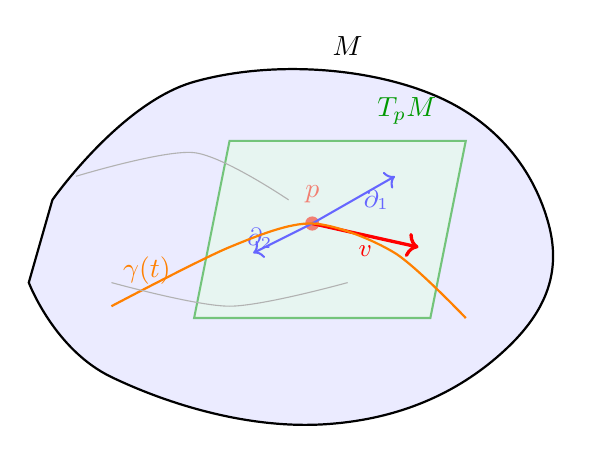
\begin{tikzpicture}[scale=1.5]
    % Manifold M (curved surface)
    \draw[thick,fill=blue!8] plot[smooth,tension=0.7] coordinates {
        (-2.0,0.5) (-0.8,1.5) (1.2,1.4) (2.2,0.3) 
        (1.8,-0.8) (0.3,-1.4) (-1.5,-1.0) (-2.2,-0.2)
    } -- cycle;
    \node at (0.5,1.8) {$M$};
    
    % Point p
    \fill[red] (0.2,0.3) circle (0.06);
    \node[red] at (0.2,0.55) {$p$};
    
    % Tangent plane at p
    \draw[green!60!black,fill=green!10,opacity=0.5] 
        (-0.8,-0.5) -- (1.2,-0.5) -- (1.5,1.0) -- (-0.5,1.0) -- cycle;
    \node[green!60!black] at (1.0,1.25) {$T_pM$};
    
    % Tangent vector
    \draw[->,red,very thick] (0.2,0.3) -- (1.1,0.1) 
        node[midway,below,font=\small] {$v$};
    
    % Coordinate basis
    \draw[->,blue!60] (0.2,0.3) -- (0.9,0.7) 
        node[midway,right,font=\small] {$\pd_1$};
    \draw[->,blue!60] (0.2,0.3) -- (-0.3,0.05) 
        node[midway,left,font=\small] {$\pd_2$};
    
    % Curve through p
    \draw[orange,thick] plot[smooth] coordinates {
        (-1.5,-0.4) (-0.5,0.1) (0.2,0.3) (0.9,0.05) (1.5,-0.5)
    };
    \node[orange] at (-1.2,-0.1) {$\gamma(t)$};
    
    % Flow lines on manifold
    \draw[gray!60,thin] plot[smooth] coordinates {
        (-1.8,0.7) (-0.8,0.9) (0.0,0.5)
    };
    \draw[gray!60,thin] plot[smooth] coordinates {
        (-1.5,-0.2) (-0.5,-0.4) (0.5,-0.2)
    };
\end{tikzpicture}
\caption{二维流形 $M$ 在点 $p$ 处的切空间 $T_pM$。$T_pM$ 是流形在 $p$ 点的"最佳线性近似"——一个二维向量平面。切向量 $v$ 可以分解为坐标基 $\{\pd_1,\pd_2\}$ 的线性组合。通过 $p$ 的曲线 $\gamma(t)$ 在 $p$ 点的切向量正是 $v$。}
\label{fig:tangent_space}
\end{figure}

\subsection{切空间与坐标变换}

\begin{definition}[切空间]
点 $p \in M$ 处所有切向量的集合记作 $T_pM$，称为 $M$ 在 $p$ 点的\textbf{切空间} (tangent space)。$T_pM$ 是一个 $n$ 维实向量空间，其维数与流形 $M$ 的维数相同。
\end{definition}

\begin{property}[切向量的坐标变换]
设 $(U, x^\mu)$ 和 $(\tilde{U}, \tilde{x}^\mu)$ 是包含 $p$ 的两个坐标卡。同一向量 $v \in T_pM$ 在两组坐标系的分量之间的变换规则为：
\begin{equation}
    \tilde{v}^\mu = \frac{\pd \tilde{x}^\mu}{\pd x^\nu} \, v^\nu, \quad v^\mu = \frac{\pd x^\mu}{\pd \tilde{x}^\nu} \, \tilde{v}^\nu.
\end{equation}
其中 Jacobi 矩阵 $\frac{\pd \tilde{x}^\mu}{\pd x^\nu}$ 在点 $p$ 处取值。这就是物理学中著名的\textbf{逆变变换律} (contravariant transformation law)——"逆变"意味着分量变换的方式与基向量的变换方式"相反"。
\end{property}

\begin{remark}[为什么称为"逆变"？]
坐标基向量 $\pd_\mu$ 在坐标变换下按 $\pd_\mu = \frac{\pd \tilde{x}^\nu}{\pd x^\mu} \tilde{\pd}_\nu$ 变换（系数是 Jacobi 矩阵的转置），而切向量的分量 $v^\mu$ 按 $\tilde{v}^\mu = \frac{\pd \tilde{x}^\mu}{\pd x^\nu} v^\nu$ 变换（系数是 Jacobi 矩阵本身）。这两种变换"方向相反"——因此被称为"逆"变（contra-variant）。与之相对，余向量的分量按协变 (co-variant) 方式变换：$\tilde{\omega}_\mu = \frac{\pd x^\nu}{\pd \tilde{x}^\mu} \omega_\nu$。
\end{remark}

\subsection{余切空间与余向量}

\begin{definition}[余切空间]
切空间 $T_pM$ 的\textbf{对偶空间} (dual space) 记作 $T_p^*M$，称为 $M$ 在 $p$ 点的\textbf{余切空间} (cotangent space)。$T_p^*M$ 中的元素 $\omega$ 是切空间上的线性泛函：
\begin{equation}
    \omega: T_pM \to \mathbb{R}, \quad \omega(av + bw) = a \, \omega(v) + b \, \omega(w).
\end{equation}
$T_p^*M$ 中的元素称为\textbf{余向量} (covector) 或 \textbf{1-形式} (1-form) \cite{Reall_Part3_GR}。
\end{definition}

一个特别重要的余向量是函数的\textbf{全微分}。对任意光滑函数 $f \in C^\infty(M)$，其在 $p$ 点的微分 $\dd f|_p \in T_p^*M$ 定义为：
\begin{equation}
    (\dd f|_p)(v) = v(f), \quad \forall v \in T_pM.
\end{equation}
在坐标卡中，$\{\dd x^1|_p, \ldots, \dd x^n|_p\}$ 构成 $T_p^*M$ 的一组基（称为坐标余基），且满足对偶关系：
\begin{equation}
    \dd x^\mu|_p (\pd_\nu|_p) = \delta^\mu_\nu.
\end{equation}

\begin{property}[余向量的坐标变换]
余向量 $\omega \in T_p^*M$ 的分量在坐标变换下的变换规则为：
\begin{equation}
    \tilde{\omega}_\mu = \frac{\pd x^\nu}{\pd \tilde{x}^\mu} \, \omega_\nu.
\end{equation}
这称为\textbf{协变变换律} (covariant transformation law)。注意这里的系数是逆 Jacobi 矩阵 $\frac{\pd x^\nu}{\pd \tilde{x}^\mu}$，而非正 Jacobi 矩阵。
\end{property}

\subsection{切丛与向量场}

\begin{definition}[切丛与向量场]
流形 $M$ 的\textbf{切丛} (tangent bundle) 是所有切空间的不交并：
\begin{equation}
    TM = \bigsqcup_{p \in M} T_pM.
\end{equation}
$TM$ 本身是一个 $2n$ 维光滑流形。$M$ 上的一个\textbf{光滑向量场} $X$ 是切丛的一个光滑截面，即对每个 $p \in M$，光滑地指定一个切向量 $X_p \in T_pM$。$M$ 上全体光滑向量场的集合记作 $\mathfrak{X}(M)$。
\end{definition}

\begin{remark}
切丛的概念在现代物理学中广泛出现：粒子的\textbf{相空间}是位形空间的余切丛 $T^*Q$；规范场是主丛上的联络；Higgs 场是伴丛的截面。所有这些构造都建立在切丛和余切丛的基础之上。
\end{remark}

\section{张量的定义与张量代数}

\subsection{从多重线性映射到张量}

余向量将单个切向量映射为实数。自然的推广是考虑接受多个切向量和余向量的多重线性映射——这就是\textbf{张量}。

\begin{definition}[$(r,s)$ 型张量]
点 $p \in M$ 处的一个 $(r,s)$ 型\textbf{张量} (tensor) 是一个多重线性映射：
\begin{equation}
    T: \underbrace{T_p^*M \times \cdots \times T_p^*M}_{r \text{ 个副本}} \times \underbrace{T_pM \times \cdots \times T_pM}_{s \text{ 个副本}} \to \mathbb{R},
\end{equation}
它在每一个变量上都是线性的。$r$ 称为\textbf{逆变阶数} (contravariant order)，$s$ 称为\textbf{协变阶数} (covariant order)，总阶数 $r+s$ 称为张量的\textbf{秩} (rank)。
\end{definition}

在分量表示中，$(r,s)$ 型张量由 $n^{r+s}$ 个分量 $T^{\mu_1\cdots\mu_r}{}_{\nu_1\cdots\nu_s}$ 完全确定，这些分量满足特定的坐标变换规则（见下文）。

\begin{figure}[htbp]
\centering
\begin{tikzpicture}[scale=1.1]
    % Title
    \node[font=\large\bfseries] at (0,2.5) {张量的可视化};
    
    % (0,0) type - scalar
    \fill[blue!30] (-3,1) circle (0.6);
    \node at (-3,1) {$f$};
    \node at (-3,0.2) {标量 $(0,0)$};
    
    % (1,0) type - vector
    \draw[->,red,very thick] (0,1) -- (1.5,1.8);
    \fill[red] (0,1) circle (0.06);
    \node at (1.0,2.1) {$v^\mu$};
    \node at (0.5,0.2) {向量 $(1,0)$};
    
    % (0,1) type - covector
    \draw[green!50!black,very thick] (3,1.8) -- (4.5,1);
    \draw[green!50!black,dashed] (3,1) -- (3,1.8);
    \draw[green!50!black,dashed] (4.5,1) -- (4.5,1.8);
    \node at (4.0,1.0) {$\omega_\mu$};
    \node at (3.5,0.2) {余向量 $(0,1)$};
    
    % (0,2) type - metric
    \draw[blue!60,thick] (-3,-0.5) -- (-4.5,-1.5);
    \draw[blue!60,thick] (-3,-0.5) -- (-2.5,-1.8);
    \draw[blue!60,thick] (-3,-0.5) -- (-1.2,-1.3);
    \node at (-3,-2.2) {度规 $g_{\mu\nu}$ $(0,2)$};
    
    % (1,1) type - linear map
    \draw[->,purple,thick] (1.5,-0.5) -- (0.5,-1.5);
    \fill[purple] (1.5,-0.5) circle (0.06);
    \node at (1.5,-2.2) {线性映射 $L^\mu{}_\nu$ $(1,1)$};
    
    % (1,3) type - Riemann tensor
    \node at (5,-0.5) {$\cdots$};
    \node at (5,-2.2) {$R^\rho{}_{\sigma\mu\nu}$ $(1,3)$};
\end{tikzpicture}
\caption{不同秩的张量对应不同类型的几何对象。标量（秩 0）是流形上的函数；向量（秩 1）是切空间中的元素；度规张量（秩 2）定义了内积；黎曼曲率张量（秩 4）描述了空间的弯曲。张量的阶数越高，编码的几何信息越丰富。}
\label{fig:tensor_types}
\end{figure}

\begin{itemize}
    \item $(0,0)$ 型：标量函数 $f \in C^\infty(M)$——一个不依赖于坐标系选择的数
    \item $(1,0)$ 型：切向量 $v \in T_pM$——流形上的"方向"
    \item $(0,1)$ 型：余向量 $\omega \in T_p^*M$——切向量上的线性泛函
    \item $(1,1)$ 型：线性变换 $L: T_pM \to T_pM$——如能量-动量张量的"1上1下"形式
    \item $(0,2)$ 型：双线性型——度规张量 $g_{\mu\nu}$ 是典型例子
    \item $(2,0)$ 型：逆度规 $g^{\mu\nu}$——在缩并中与度规配对
    \item $(1,3)$ 型：黎曼曲率张量 $R^\rho{}_{\sigma\mu\nu}$——编码了所有曲率信息
\end{itemize}

\subsection{张量积}

\begin{definition}[张量积]
设 $T$ 是 $(r,s)$ 型张量，$S$ 是 $(p,q)$ 型张量。其\textbf{张量积} (tensor product) $T \otimes S$ 是一个 $(r+p, s+q)$ 型张量，定义为：
\begin{equation}
    (T \otimes S)^{\mu_1\cdots\mu_r\nu_1\cdots\nu_p}{}_{\rho_1\cdots\rho_s\sigma_1\cdots\sigma_q}
    = T^{\mu_1\cdots\mu_r}{}_{\rho_1\cdots\rho_s} \, S^{\nu_1\cdots\nu_p}{}_{\sigma_1\cdots\sigma_q}.
\end{equation}
\end{definition}

\begin{remark}[张量代数的分次结构]
全体张量构成一个\textbf{分次代数} (graded algebra)：$\mathcal{T}(M) = \bigoplus_{r,s \geq 0} \mathcal{T}^{(r,s)}(M)$。分次乘法的规则是 $\mathcal{T}^{(r,s)} \otimes \mathcal{T}^{(p,q)} \subseteq \mathcal{T}^{(r+p,s+q)}$。张量积满足结合性，但不交换（除非其中一个张量的秩为 0）\cite{TensorFields2017}。这种分次结构使得张量代数成为一个强大的代数系统——物理量在相互作用下"增加阶数"，但系统始终保持在张量代数的框架内。
\end{remark}

\subsection{缩并：指标的求和}

\begin{definition}[缩并]
设 $T$ 是 $(r,s)$ 型张量（$r \geq 1$, $s \geq 1$）。对第 $i$ 个逆变指标和第 $j$ 个协变指标进行\textbf{缩并} (contraction) 得到一个 $(r-1, s-1)$ 型张量。在分量形式下：
\begin{equation}
    (\operatorname{tr}_{ij} T)^{\mu_1\cdots\hat{\mu}_i\cdots\mu_r}{}_{\nu_1\cdots\hat{\nu}_j\cdots\nu_s}
    = T^{\mu_1\cdots\lambda\cdots\mu_r}{}_{\nu_1\cdots\lambda\cdots\nu_s},
\end{equation}
其中 $\hat{\cdot}$ 表示被移除的指标，Einstein 求和约定意味着对重复指标 $\lambda$ 自动求和 \cite{Reall_Part3_GR}。
\end{definition}

\begin{itemize}
    \item 线性变换的迹：$\operatorname{tr}(L) = L^\mu{}_\mu$（$(1,1)$ 型缩并为 $(0,0)$ 型标量）
    \item 向量与余向量的自然配对：$\omega(v) = \omega_\mu v^\mu$（$(0,1)$ 与 $(1,0)$ 缩并）
    \item 里奇张量：$R_{\mu\nu} = R^\lambda{}_{\mu\lambda\nu}$（$(1,3)$ 型的一次缩并为 $(0,2)$ 型）
    \item 标量曲率：$R = g^{\mu\nu} R_{\mu\nu}$（先缩并再缩并 = 两次缩并）
\end{itemize}

\begin{remark}
缩并的本质是"求和"——将一个逆变指标和一个协变指标配对后求和，从而消去这两个指标。从几何上看，缩并对应的是"取迹"操作。缩并是唯一能够自然地（即与基的选择无关地）将不同指标"配对"的方式。值得注意的是，你不能将两个逆变指标（或两个协变指标）直接缩并——你需要先用度规升降其中一个指标。
\end{remark}

\subsection{抽象指标记法}

现代微分几何和广义相对论中广泛使用\textbf{抽象指标记法} (abstract index notation)，由 Penrose 推广 \cite{Reall_Part3_GR}。在这一记法中，张量 $T$ 写为 $T^{ab}{}_{c}$（其中拉丁字母 $a,b,c$ 是抽象指标），但这些指标并不代表某个特定坐标系下的分量——它们只是"标记张量槽位"的标签。

这种记法的优势在于：它允许我们使用指标运算的简便性，同时保持几何的不变性。方程 $T^{ab}{}_{c} = U^{a}{}_{cd} V^{bd}$ 既是几何陈述（"两个张量相等"），又是分量计算指令（"对指标进行缩并求和"）。在广义相对论和量子场论中，希腊字母 $\mu,\nu$ 通常表示具体坐标下的分量，拉丁字母 $a,b,c$ 表示抽象指标。

\section{张量的坐标变换规则}

张量的定义特性是其分量在坐标变换下的变换规则。这是张量概念的"操作定义"。

\begin{property}[张量变换律]
设 $T$ 是 $(r,s)$ 型张量。在坐标变换 $x \mapsto \tilde{x}$ 下，其分量变换为：
\begin{equation}
    \tilde{T}^{\mu_1\cdots\mu_r}{}_{\nu_1\cdots\nu_s}
    = \frac{\pd \tilde{x}^{\mu_1}}{\pd x^{\rho_1}} \cdots \frac{\pd \tilde{x}^{\mu_r}}{\pd x^{\rho_r}}
    \cdot \frac{\pd x^{\sigma_1}}{\pd \tilde{x}^{\nu_1}} \cdots \frac{\pd x^{\sigma_s}}{\pd \tilde{x}^{\nu_s}}
    \cdot T^{\rho_1\cdots\rho_r}{}_{\sigma_1\cdots\sigma_s}.
\end{equation}
\end{property}

这条规则告诉我们：每一个上指标乘以 Jacobi 矩阵 $\frac{\pd \tilde{x}}{\pd x}$，每一个下指标乘以逆 Jacobi 矩阵 $\frac{\pd x}{\pd \tilde{x}}$。

\begin{remark}[如何判断一个量是不是张量]
在广义相对论中，一个最基本的直观判别法是：如果一个多重指标的量在坐标变换下按照上述规则变换，它就是一个张量；否则就不是。这是张量的\textbf{操作定义}。特别地，Christoffel 符号 $\Gamma^\lambda{}_{\mu\nu}$ 不按张量的方式变换（它多出了一项二阶导数的非齐次项），因此它\textbf{不是}张量——这个事实在后续章节中将反复强调。
\end{remark}

\section{对称张量与反对称张量}

\begin{definition}[对称与反对称张量]
一个 $(0,2)$ 型张量 $T_{\mu\nu}$ 称为：
\begin{itemize}
    \item \textbf{对称的} (symmetric)，如果 $T_{\mu\nu} = T_{\nu\mu}$
    \item \textbf{反对称的} (antisymmetric/skew-symmetric)，如果 $T_{\mu\nu} = -T_{\nu\mu}$
\end{itemize}
\end{definition}

对称化与反对称化操作可以推广到任意 $(0,k)$ 型张量：

\begin{definition}[对称化与反对称化]
对 $(0,k)$ 型张量 $T_{\mu_1\cdots\mu_k}$：
\begin{align}
    T_{(\mu_1\cdots\mu_k)} &= \frac{1}{k!} \sum_{\sigma \in S_k} T_{\mu_{\sigma(1)}\cdots\mu_{\sigma(k)}}, \quad\text{（对称化：$k!$ 个排列的平均）} \
    T_{[\mu_1\cdots\mu_k]} &= \frac{1}{k!} \sum_{\sigma \in S_k} \operatorname{sgn}(\sigma) \, T_{\mu_{\sigma(1)}\cdots\mu_{\sigma(k)}}, \quad\text{（反对称化：$k!$ 个带符号排列的平均）}
\end{align}
其中 $S_k$ 是 $k$ 个元素的置换群，$\operatorname{sgn}(\sigma)$ 是置换的符号（偶置换为 $+1$，奇置换为 $-1$）。
\end{definition}

\begin{property}[反对称张量的独立分量数]
$n$ 维空间上的 $(0,k)$ 型完全反对称张量的独立分量数为 $\binom{n}{k} = \frac{n!}{k!(n-k)!}$。特别地，$k > n$ 时反对称张量恒为零（因为没有足够的维度来产生非零的完全反对称组合）。
\end{property}

\section{度规张量：连接几何与物理}

度规张量是微分几何与广义相对论中最重要的张量——它将流形的微分拓扑结构转化为有"长度"和"角度"的黎曼几何结构。

\begin{definition}[度规张量]
$M$ 上的一个\textbf{度规张量} (metric tensor) $g$ 是一个对称的、非退化的 $(0,2)$ 型光滑张量场：
\begin{equation}
    g = g_{\mu\nu} \, \dd x^\mu \otimes \dd x^\nu, \quad g_{\mu\nu} = g_{\nu\mu}, \quad \det(g_{\mu\nu}) \neq 0.
\end{equation}
\end{definition}

度规张量赋予流形上每一点切空间中的一个内积（可能是不定的）：
\begin{equation}
    \langle u, v \rangle_g = g_{\mu\nu} u^\mu v^\nu.
\end{equation}

\begin{definition}[号差与洛伦兹流形]
在标准正交基下，度规的对角元素中正负号的数量差称为度规的\textbf{号差} (signature)。如果号差为 $(-,+,+,+)$ 或 $(+,-,-,-)$，则称度规具有\textbf{洛伦兹号差} (Lorentzian signature)。配备了洛伦兹度规的流形称为\textbf{洛伦兹流形}。在广义相对论中，时空被建模为一个四维洛伦兹流形 $(\mathcal{M}, g)$ \cite{Wald1984}。
\end{definition}

根据号差，切向量可以分类为：
\begin{itemize}
    \item $g_{\mu\nu} v^\mu v^\nu < 0$：\textbf{类时} (timelike) —— 物理粒子的世界线
    \item $g_{\mu\nu} v^\mu v^\nu = 0$：\textbf{类光} (lightlike/null) —— 光子的世界线
    \item $g_{\mu\nu} v^\mu v^\nu > 0$：\textbf{类空} (spacelike) —— 不能因果相连的事件间隔
\end{itemize}

\begin{definition}[逆度规]
由非退化性，度规矩阵 $g_{\mu\nu}$ 可逆。其逆记作 $g^{\mu\nu}$，满足 $g^{\mu\lambda} g_{\lambda\nu} = \delta^\mu_\nu$。$g^{\mu\nu}$ 是一个 $(2,0)$ 型对称张量，称为\textbf{逆度规} (inverse metric)。
\end{definition}

度规和逆度规提供了指标升降的标准方式：
\begin{equation}
    v_\mu = g_{\mu\nu} v^\nu, \quad T^{\mu\nu} = g^{\mu\rho} g^{\nu\sigma} T_{\rho\sigma}, \quad R = g^{\mu\nu} R_{\mu\nu}.
\end{equation}
指标升降使得我们可以在协变形式和逆变形式之间自由切换，这是张量分析中最常用的技术操作。

\begin{note}[物理意义]
在广义相对论中，度规张量扮演着双重角色：
\begin{enumerate}
    \item \textbf{几何角色}：它定义了时空中"距离"的概念——类时曲线上的固有时间隔 $\dd \tau^2 = -g_{\mu\nu} \dd x^\mu \dd x^\nu / c^2$
    \item \textbf{动力学角色}：度规是引力场的\textbf{动力学变量}——爱因斯坦场方程是关于 $g_{\mu\nu}$ 的偏微分方程。在这个意义上，度规就是"引力势"的广义相对论推广。
\end{enumerate}
\end{note}

\begin{itemize}
    \item \textbf{闵可夫斯基度规}（平坦时空）：
    \begin{equation}
        \dd s^2 = -\dd t^2 + \dd x^2 + \dd y^2 + \dd z^2, \quad g_{\mu\nu} = \operatorname{diag}(-1, +1, +1, +1)
    \end{equation}
    \item \textbf{施瓦西度规}（球对称黑洞外部）：
    \begin{equation}
        \dd s^2 = -\left(1 - \frac{2GM}{r}\right) \dd t^2 + \left(1 - \frac{2GM}{r}\right)^{-1} \dd r^2 + r^2(\dd\theta^2 + \sin^2\theta\,\dd\phi^2)
    \end{equation}
    注意：当 $M=0$ 时，施瓦西度规在 $r \to \infty$ 处约化为闵可夫斯基度规——这体现了广义相对论在弱场极限下回到狭义相对论。
\end{itemize}

\section{张量密度}

许多重要的物理量（如拉格朗日密度 $\sqrt{-g} \Lag$、作用量中的体积元 $\sqrt{-g} \dd^4 x$）涉及度规的行列式。这引入了张量密度的概念。

\begin{definition}[张量密度]
一个\textbf{权重为 $w$ 的 $(r,s)$ 型张量密度}（或称为相对张量）是一个在坐标变换下按照以下规则变换的多重指标量：
\begin{equation}
    \tilde{\mathfrak{T}}^{\mu_1\cdots}{}_{\nu_1\cdots}
    = \left|\det\!\left(\frac{\pd x}{\pd \tilde{x}}\right)\right|^{w}
    \frac{\pd \tilde{x}^{\mu_1}}{\pd x^{\rho_1}} \cdots
    \mathfrak{T}^{\rho_1\cdots}{}_{\sigma_1\cdots}.
\end{equation}
特别地，$\sqrt{-g}$ 是权重为 $+1$ 的标量密度；$1/\sqrt{-g}$ 是权重为 $-1$ 的标量密度。
\end{definition}

\begin{remark}
在广义相对论中，体积元 $\dd^4 x$ 本身不是标量（在坐标变换下它乘上 Jacobi 行列式），但组合 $\sqrt{-g} \, \dd^4 x$ 是一个真正的标量。这使得作用量 $S = \int \Lag \sqrt{-g} \, \dd^4 x$ 在任意坐标变换下都是不变的——物理定律的协变性由此得到保证。
\end{remark}

\section{Levi-Civita 张量与定向}

\begin{definition}[Levi-Civita 符号与张量]
\textbf{Levi-Civita 符号} $\tilde{\varepsilon}_{\mu_1\cdots\mu_n}$ 是满足 $\tilde{\varepsilon}_{12\cdots n} = +1$ 且关于任意两个指标的交换完全反对称的量。然而它\textbf{不是}一个张量——它是一个权重为 $-1$ 的张量密度。

真正的\textbf{Levi-Civita 张量}（或体积元形式）是：
\begin{equation}
    \varepsilon_{\mu_1\cdots\mu_n} = \sqrt{|g|} \, \tilde{\varepsilon}_{\mu_1\cdots\mu_n}, \quad
    \varepsilon^{\mu_1\cdots\mu_n} = \frac{1}{\sqrt{|g|}} \, \tilde{\varepsilon}^{\mu_1\cdots\mu_n}.
\end{equation}
其中 $g = \det(g_{\mu\nu})$。注意 $\varepsilon_{\mu_1\cdots\mu_n}$ 是真正的 $(0,n)$ 型反对称张量。
\end{definition}

Levi-Civita 张量在广义相对论的多处都出现：体积分（$\dd V = \varepsilon_{\mu_1\cdots\mu_n} \dd x^{\mu_1} \wedge \cdots \wedge \dd x^{\mu_n}$）、Hodge 对偶（第 \ref{chap:forms} 章）、以及在引力作用量中引入 Gauss--Bonnet 拓扑项。

\section{算例演练 (Worked Examples)}

下面通过大量具体算例来巩固本章的所有核心概念。所有算例均尽可能详细地展示中间步骤。

\subsection{Einstein 求和约定}

\
\begin{equation}
    A^\mu B_\mu = A^0 B_0 + A^1 B_1 + A^2 B_2 + A^3 B_3.
\end{equation}
重复的上下指标 $\mu$ 自动求和，求和范围由时空维数决定（此处四维）。注意 $A^\mu$ 和 $A_\mu$ 是不同的对象（逆变 vs 协变）。

\
\begin{equation}
    \delta^\mu_\mu = \delta^0_0 + \delta^1_1 + \delta^2_2 + \delta^3_3 = 1 + 1 + 1 + 1 = 4.
\end{equation}
Kronecker delta 的完全缩并等于时空维数 $n$。在 $n$ 维空间中：$\delta^\mu_\mu = n$。这在迹运算中经常用到。

\
\begin{equation}
    \delta^\mu_\nu A^\nu = A^\mu.
\end{equation}
这是因为 $\delta^\mu_\nu = 1$ 仅当 $\mu = \nu$，因此求和只剩下 $\nu = \mu$ 的一项。$\delta^\mu_\nu$ 的作用是"替换指标"。

\
设 Minkowski 度规 $\eta_{\mu\nu} = \text{diag}(-1,+1,+1,+1)$，计算 $\eta_{\mu\nu} \eta^{\mu\nu}$：
\begin{equation}
    \eta_{\mu\nu} \eta^{\mu\nu} = \eta_{\mu\nu} \eta^{\mu\nu} = \delta^\mu_\mu = 4.
\end{equation}
更详细地：
\begin{equation}
    \eta^{\mu\nu} \eta_{\nu\rho} = \delta^\mu_\rho.
\end{equation}
验证 $\mu = 0, \rho = 0$：$\eta^{0\nu} \eta_{\nu 0} = \eta^{00} \eta_{00} = (-1) \times (-1) = 1 = \delta^0_0$。$\checkmark$

\
\begin{equation}
    g_{\mu\nu} A^\mu B^\nu = A_0 B_0 - A_1 B_1 - A_2 B_2 - A_3 B_3 \quad \text{（号差 $(-,+,+,+)$）}.
\end{equation}
展开：$g_{00}A^0 B^0 + g_{11}A^1 B^1 + g_{22}A^2 B^2 + g_{33}A^3 B^3 = -A^0 B^0 + A^1 B^1 + A^2 B^2 + A^3 B^3$。

\begin{remark}[求和约定的哑指标与自由指标]
在表达式中，重复且配对（一上一下或两个都在位置不变的情况下由度规连接）的指标称为\textbf{哑指标} (dummy index)，可以任意重命名而不改变含义。例如 $A_\mu B^\mu = A_\nu B^\nu$。未配对的指标（如 $A^\mu$ 中的 $\mu$）称为\textbf{自由指标} (free index)，等式两侧必须匹配。
\end{remark}

\subsection{张量积算例}

\
设 $A^\mu = (1, 2, 0, -1)$ 和 $B^\mu = (0, 3, 1, 0)$ 为 Minkowski 时空中的两个切向量。其张量积 $T^{\mu\nu} = A^\mu B^\nu$ 是一个 $(2,0)$ 型张量，分量为 $4 \times 4 = 16$ 个：
\begin{equation}
    T^{\mu\nu} = A^\mu B^\nu = 
    \begin{pmatrix}
        0 & 3  & 1  & 0 \\
        0 & 6  & 2  & 0 \\
        0 & 0  & 0  & 0 \\
        0 & -3 & -1 & 0
    \end{pmatrix}.
\end{equation}
其中 $T^{01} = A^0 B^1 = 1 \times 3 = 3$，$T^{10} = A^1 B^0 = 2 \times 0 = 0$，等等。注意 $T^{\mu\nu} \neq T^{\nu\mu}$ 一般情况（张量积不交换）。

\
度规 $g_{\mu\nu}$ 是 $(0,2)$ 型，切向量 $V^\rho$ 是 $(1,0)$ 型。其张量积 $S^\rho{}_{\mu\nu} = V^\rho g_{\mu\nu}$ 是一个 $(1,2)$ 型张量，有 $4 \times 4 \times 4 = 64$ 个分量。具体写出一项：
\begin{equation}
    S^1{}_{00} = V^1 g_{00} = V^1 \times (-1) = -V^1.
\end{equation}

\
将 $\delta^\mu_\nu$（$(1,1)$ 型）与向量 $V^\rho$ 做张量积：
\begin{equation}
    W^{\mu\rho}{}_{\nu} = \delta^\mu_\nu V^\rho.
\end{equation}
然后对 $\mu$ 和 $\nu$ 缩并：$W^{\mu\rho}{}_{\mu} = \delta^\mu_\mu V^\rho = 4 V^\rho$。迹使结果放大了 $n$ 倍。

\subsection{缩并算例}

\
设 $L^\mu{}_\nu$ 是一个 $(1,1)$ 型张量，表示为 $4 \times 4$ 矩阵。其缩并（迹）为：
\begin{equation}
    \text{tr}(L) = L^\mu{}_\mu = L^0{}_0 + L^1{}_1 + L^2{}_2 + L^3{}_3.
\end{equation}
具体数值例子：若 $L^\mu{}_\nu = \text{diag}(2, -1, 3, 0)$，则 $\text{tr}(L) = 2 + (-1) + 3 + 0 = 4$。

\
里奇张量 $R_{\mu\nu}$ 是 Riemann 张量的缩并 $R^\lambda{}_{\mu\lambda\nu}$。在四维中：
\begin{equation}
    R_{00} = R^0{}_{000} + R^1{}_{010} + R^2{}_{020} + R^3{}_{030}.
\end{equation}
每一项都是 Riemann 张量的一个具体分量。例如 $R^1{}_{010}$ 表示沿 $x^0$ 和 $x^1$ 方向的曲率对 $x^1$ 基向量的效应。

\
从里奇张量进一步缩并得到标量曲率 $R = g^{\mu\nu} R_{\mu\nu}$：
\begin{equation}
    \begin{aligned}
        R &= g^{00} R_{00} + g^{11} R_{11} + g^{22} R_{22} + g^{33} R_{33} \
          &= -R_{00} + R_{11} + R_{22} + R_{33} \quad \text{（Minkowski 背景）}.
    \end{aligned}
\end{equation}

\subsection{坐标变换算例}

\
设 $\mathbb{R}^2$ 上，笛卡尔坐标 $(x, y)$ 与极坐标 $(r, \theta)$ 的关系为 $x = r\cos\theta$, $y = r\sin\theta$。一个切向量 $V$ 在笛卡尔坐标系下的分量为 $V^x, V^y$，在极坐标下的分量 $V^r, V^\theta$ 由逆变变换律给出：
\begin{equation}
    \begin{pmatrix} V^r \\[2pt] V^\theta \end{pmatrix}
    = \begin{pmatrix}
        \frac{\pd r}{\pd x} & \frac{\pd r}{\pd y} \\[6pt]
        \frac{\pd \theta}{\pd x} & \frac{\pd \theta}{\pd y}
    \end{pmatrix}
    \begin{pmatrix} V^x \\[2pt] V^y \end{pmatrix}.
\end{equation}
计算 Jacobi 矩阵：由 $r = \sqrt{x^2 + y^2}$ 得 $\frac{\pd r}{\pd x} = \frac{x}{r} = \cos\theta$, $\frac{\pd r}{\pd y} = \frac{y}{r} = \sin\theta$。由 $\theta = \arctan(y/x)$ 得 $\frac{\pd \theta}{\pd x} = -\frac{y}{r^2} = -\frac{\sin\theta}{r}$, $\frac{\pd \theta}{\pd y} = \frac{x}{r^2} = \frac{\cos\theta}{r}$。因此：
\begin{equation}
    \boxed{V^r = \cos\theta \, V^x + \sin\theta \, V^y, \quad V^\theta = -\frac{\sin\theta}{r} V^x + \frac{\cos\theta}{r} V^y}.
\end{equation}
这正是向量在极坐标下的分量——注意 $\theta$ 分量的量纲是 $\text{radian}/\text{长度}$，因为基向量 $\pd_\theta$ 本身带有长度量纲。

\
一个标量函数 $f(x,y) = x^2 + y^2 = r^2$ 的梯度 $\dd f$ 是余向量。在笛卡尔坐标下：$\omega_x = \pd_x f = 2x$, $\omega_y = \pd_y f = 2y$。在极坐标下由协变变换律：
\begin{equation}
    \begin{aligned}
        \omega_r &= \frac{\pd x}{\pd r} \omega_x + \frac{\pd y}{\pd r} \omega_y = \cos\theta \cdot 2x + \sin\theta \cdot 2y = 2r, \
        \omega_\theta &= \frac{\pd x}{\pd \theta} \omega_x + \frac{\pd y}{\pd \theta} \omega_y = (-r\sin\theta) \cdot 2x + (r\cos\theta) \cdot 2y = 0.
    \end{aligned}
\end{equation}
验证：$\dd f = 2r \dd r$——极坐标下梯度的 $\theta$ 分量为零，因为 $f$ 是径向对称的。

\
设 $F_{\mu\nu}$ 是 $(0,2)$ 型反对称张量，在坐标系 $x^\mu = (t, x, y, z)$ 下非零分量为 $F_{01} = E_x$, $F_{02} = E_y$, $F_{12} = -B_z$。在沿 $x$ 方向的 Lorentz boost 下，
\begin{equation}
    \tilde{t} = \gamma(t - vx), \quad \tilde{x} = \gamma(x - vt), \quad \tilde{y} = y, \quad \tilde{z} = z,
\end{equation}
其中 $\gamma = 1/\sqrt{1-v^2}$。计算 $\tilde{F}_{01}$：
\begin{equation}
    \tilde{F}_{01} = \frac{\pd x^\rho}{\pd \tilde{t}} \frac{\pd x^\sigma}{\pd \tilde{x}} F_{\rho\sigma}.
\end{equation}
非零贡献来自 Jacobi 矩阵元素。最终得到 $\tilde{F}_{01} = E_x$（不变量），$\tilde{F}_{02} = \gamma(E_y - v B_z)$——这正是电磁场在 Lorentz 变换下的变换公式（电场的一部分转化为磁场）。\textbf{张量的变换律自动给出了物理量的坐标变换}。

\subsection{对称化与反对称化算例}

\
任何 $(0,2)$ 型张量 $T_{\mu\nu}$ 可唯一分解为：
\begin{equation}
    T_{\mu\nu} = T_{(\mu\nu)} + T_{[\mu\nu]}, \quad T_{(\mu\nu)} = \frac{1}{2}(T_{\mu\nu} + T_{\nu\mu}), \quad T_{[\mu\nu]} = \frac{1}{2}(T_{\mu\nu} - T_{\nu\mu}).
\end{equation}
例如 $T_{\mu\nu} = \begin{pmatrix} 0 & 2 & -1 \ 1 & 0 & 3 \ 0 & -2 & 0 \end{pmatrix}$（以矩阵表示）。则：
\begin{equation}
    T_{(\mu\nu)} = \begin{pmatrix} 0 & 1.5 & -0.5 \ 1.5 & 0 & 0.5 \ -0.5 & 0.5 & 0 \end{pmatrix}, \quad
    T_{[\mu\nu]} = \begin{pmatrix} 0 & 0.5 & -0.5 \ -0.5 & 0 & 2.5 \ 0.5 & -2.5 & 0 \end{pmatrix}.
\end{equation}
验证：$T_{(\mu\nu)} + T_{[\mu\nu]} = T_{\mu\nu}$。$\checkmark$

\
在 $n=3$ 维空间中，$(0,3)$ 型完全反对称张量的独立分量数为 $\binom{3}{3} = 1$——只有一个独立分量！具体设 $A_{[\mu\nu\rho]}$，则所有非零分量都由 $A_{123}$ 决定：
\begin{equation}
    A_{123} = A_{231} = A_{312} = -A_{132} = -A_{213} = -A_{321}.
\end{equation}
因此 $A_{\mu\nu\rho} = A_{123} \cdot \tilde{\varepsilon}_{\mu\nu\rho}$，其中 $\tilde{\varepsilon}$ 是 Levi-Civita 符号。这正是三维空间中\textbf{轴向量} (pseudovector) 对应到 2-形式的数学基础（如磁场 $\mathbf{B}$ 对应到 $B_{ij} = \varepsilon_{ijk} B_k$）。

\
因 $g_{\mu\nu} = g_{\nu\mu}$，有：
\begin{equation}
    g_{\mu\nu} A^\mu B^\nu = g_{(\mu\nu)} A^\mu B^\nu = g_{\mu\nu} A^{(\mu} B^{\nu)}.
\end{equation}
第二个等号成立因为反对称部分与对称度规缩并的结果为 0：$g_{\mu\nu} A^{[\mu} B^{\nu]} = 0$。一般规则：$\text{对称} \times \text{反对称} = 0$（在完全缩并下）。

\subsection{指标升降算例}

\
在 Minkowski 时空 $(\eta_{\mu\nu}) = \text{diag}(-1,+1,+1,+1)$ 中，设 $V^\mu = (V^0, V^1, V^2, V^3) = (3, 1, -2, 0)$。降指标：
\begin{equation}
    V_\mu = \eta_{\mu\nu} V^\nu: \quad V_0 = -V^0 = -3, \quad V_1 = V^1 = 1, \quad V_2 = V^2 = -2, \quad V_3 = V^3 = 0.
\end{equation}
即 $V_\mu = (-3, 1, -2, 0)$。再升回去：$V^\mu = \eta^{\mu\nu} V_\nu$ 得到原始分量。$\checkmark$

\
球面度规 $g_{\mu\nu} = \text{diag}(1, \sin^2\theta)$，逆度规 $g^{\mu\nu} = \text{diag}(1, 1/\sin^2\theta)$。设切向量 $V^\mu = (V^\theta, V^\phi) = (2, 3)$。降指标：
\begin{equation}
    V_\theta = g_{\theta\theta} V^\theta = 1 \times 2 = 2, \quad V_\phi = g_{\phi\phi} V^\phi = \sin^2\theta \times 3 = 3\sin^2\theta.
\end{equation}
注意 $V_\phi$ 依赖于 $\theta$——在靠近极点（$\theta \to 0$）时它趋于零。这反映了球面在极点处的坐标奇异性。

\
缩并 $\omega_\mu V^\mu$ 可以先升 $\omega$ 或先降 $V$：
\begin{equation}
    \omega_\mu V^\mu = \omega^\mu V_\mu = g^{\mu\nu} \omega_\mu V_\nu = g_{\mu\nu} \omega^\mu V^\nu.
\end{equation}
数值验证：设 $\omega_\mu = (1, 2, -1, 0)$, $V^\mu = (3, 0, 1, -2)$ 在 Minkowski 时空。$\omega_\mu V^\mu = -1 \times 3 + 2 \times 0 + (-1) \times 1 + 0 \times (-2) = -4$。先升 $\omega$：$\omega^\mu = (-1, 2, -1, 0)$，则 $\omega^\mu V_\mu = (-1) \times (-3) + 2 \times 0 + (-1) \times 1 + 0 \times (-2) = -4$。$\checkmark$

\subsection{度规及逆度规的算例}

\
施瓦西度规（$c=1$, $G=1$）：
\begin{equation}
    g_{\mu\nu} = \text{diag}\!\left(-\left(1-\frac{2M}{r}\right),\; \left(1-\frac{2M}{r}\right)^{-1},\; r^2,\; r^2\sin^2\theta\right).
\end{equation}
逆度规为各对角元的倒数：
\begin{equation}
    g^{\mu\nu} = \text{diag}\!\left(-\left(1-\frac{2M}{r}\right)^{-1},\; 1-\frac{2M}{r},\; \frac{1}{r^2},\; \frac{1}{r^2\sin^2\theta}\right).
\end{equation}
验证缩并：例如 $g^{11} g_{11} = (1-\frac{2M}{r}) \times (1-\frac{2M}{r})^{-1} = 1$。

\
第一章提到的球面 Christoffel 符号 $\Gamma^\phi{}_{\theta\phi} = \cot\theta$ 可以通过 Levi-Civita 公式直接验证：
\begin{equation}
    \Gamma^\phi{}_{\theta\phi} = \frac{1}{2} g^{\phi\rho} (\pd_\theta g_{\phi\rho} + \pd_\phi g_{\theta\rho} - \pd_\rho g_{\theta\phi}).
\end{equation}
由于 $g_{\theta\phi} = 0$，只有 $\rho = \phi$ 项非零：
\begin{equation}
    \Gamma^\phi{}_{\theta\phi} = \frac{1}{2} g^{\phi\phi} \pd_\theta g_{\phi\phi} = \frac{1}{2} \cdot \frac{1}{\sin^2\theta} \cdot 2\sin\theta\cos\theta = \cot\theta. \quad \checkmark
\end{equation}


\begin{note}[物理意义：本章总结]
本章建立的所有张量运算——求和约定、张量积、缩并、坐标变换、对称化/反对称化、指标升降——构成了广义相对论日常计算的语言。在后续章节中：
\begin{itemize}
    \item \textbf{联络系数} $\Gamma^\lambda{}_{\mu\nu}$ 由度规的导数通过升降指标构造（第 \ref{chap:connection} 章）
    \item \textbf{曲率张量} $R^\rho{}_{\sigma\mu\nu}$ 的缩并产生里奇张量和爱因斯坦张量（第 \ref{chap:curvature} 章）
    \item \textbf{测地线方程}使用 Christoffel 符号进行指标缩并（第 \ref{chap:geodesic} 章）
    \item \textbf{爱因斯坦场方程} $G_{\mu\nu} = 8\pi G T_{\mu\nu}$ 中的每一项都是通过张量运算构造的（第 10 章）
\end{itemize}
\end{note}

\begin{figure}[htbp]
\centering
\begin{tikzpicture}[scale=1.2]
    % Left: 笛卡尔坐标
    \draw[->,thick] (-1.5,0) -- (2.5,0) node[right] {$x$};
    \draw[->,thick] (0,-1.5) -- (0,2.5) node[above] {$y$};
    
    % Vector V
    \draw[->,red,very thick] (0,0) -- (2.0,1.0);
    \node[red] at (2.2,1.2) {$V$};
    \node[red,font=\footnotesize] at (1.5,0.3) {$V^\mu=(V^x,V^y)$};
    
    % Grid
    \draw[gray!30,step=0.5] (-1.5,-1.5) grid (2.5,2.5);
    
    % Right: 极坐标
    \draw[->,thick] (5.5,0) -- (9.5,0) node[right] {$r$};
    \draw[->,thick] (7,1.5) -- (7,2.5);
    
    % Radial lines
    \foreach \a in {0,30,...,330} {
        \draw[gray!30] (7,0) -- ++(\a:2.0);
    }
    % Circles
    \foreach \r in {0.5,1.0,1.5,2.0} {
        \draw[gray!30] (7,0) circle (\r);
    }
    
    % Same vector V in polar coords
    \draw[->,red,very thick] (7,0) -- (9.0,1.0);
    \node[red] at (9.2,1.2) {$V$};
    \node[red,font=\footnotesize] at (8.2,0.3) {$\tilde{V}^\mu=(V^r,V^\theta)$};
    
    % Transformation arrow between
    \draw[->,teal,very thick,dashed] (4.5,0.5) -- (5.0,0.5);
    \node[teal] at (3.5,0.8) {$\tilde{V}^\mu = \frac{\pd \tilde{x}^\mu}{\pd x^\nu} V^\nu$};
    
    \node at (0.5,-2.0) {笛卡尔坐标};
    \node at (7.0,-2.0) {极坐标};
\end{tikzpicture}
\caption{同一向量 $V$ 在不同坐标系下的分量表示。左：笛卡尔坐标基 $\{\pd_x,\pd_y\}$ 下的分量 $(V^x, V^y)$。右：极坐标基 $\{\pd_r,\pd_\theta\}$ 下的分量 $(V^r, V^\theta)$。两组分量通过逆变变换律联系：$\tilde{V}^\mu = \frac{\pd \tilde{x}^\mu}{\pd x^\nu} V^\nu$。注意 $V^\theta$ 的量纲与 $V^x$ 不同——因为极坐标基向量 $\pd_\theta$ 的长度随 $r$ 变化。}
\label{fig:tensor_transform}
\end{figure}

\begin{note}[物理意义]
张量是物理学定律的通用语言，而爱因斯坦的广义协变性原理在数学上等价于"所有物理定律必须表达为张量方程"。张量方程的一个关键性质是\textbf{协变性}：如果一个张量方程在一个坐标系中成立，那么它在所有坐标系中都成立——只要你在每个坐标系中正确地计算了分量。这确保了物理定律不依赖于我们选择的描述方式。
\end{note}
  % 张量与张量代数
% chapter04.tex - 微分形式与外微分
\chapter{微分形式与外微分 (Differential Forms and Exterior Calculus)}
\label{chap:forms}

\section{为什么需要微分形式？}

\begin{note}[物理动机]
在电磁学中，我们习惯分别处理电场 $\mathbf{E}$ 和磁场 $\mathbf{B}$。但在相对论电动力学中，这两个场自然地统一为一个反对称张量 $F_{\mu\nu}$ —— 电磁场张量。类似地，Maxwell 方程的四个分量方程自然合并为两个简洁的方程。这里起作用的就是微分形式的语言：它使得反对称张量、积分、以及微分运算之间的相互作用变得极其自然。在广义相对论中，微分形式更是不可或缺 —— 从 Palatini 变分到 Cartan 结构方程，从 Chern--Simons 理论到拓扑不变量。
\end{note}

\section{外代数与楔积}

\subsection{p-形式}

\begin{definition}[$k$-形式]
流形 $M$ 上的一个\textbf{$k$-形式}（或\textbf{微分 $k$-形式}）$\omega$ 是一个光滑的完全反对称 $(0,k)$ 型张量场：
\begin{equation}
    \omega_{\mu_1\cdots\mu_k} = \omega_{[\mu_1\cdots\mu_k]}.
\end{equation}
$M$ 上全体 $k$-形式的空间记作 $\Omega^k(M)$。
\end{definition}

按此约定：
\begin{itemize}
    \item $\Omega^0(M) = C^\infty(M)$：0-形式就是光滑函数
    \item $\Omega^1(M)$：1-形式就是余向量场（余切空间的截面）
    \item $\Omega^n(M)$：$n$ 维流形上的 $n$-形式也称为\textbf{体积形式} (volume form)，因为它的独立分量只有一个
\end{itemize}

\begin{property}[$k$-形式的独立分量数]
在 $n$ 维流形上，$k$-形式的独立分量数为 $\binom{n}{k}$。因此 $\dim \Omega^k(M) = \binom{n}{k}$。特别地，当 $k > n$ 时，$\Omega^k(M) = \{0\}$（任何 $k$-形式必然为零）。
\end{property}

\subsection{楔积：反对称的张量积}

\begin{definition}[楔积]
设 $\omega \in \Omega^p(M)$ 和 $\eta \in \Omega^q(M)$。它们的\textbf{楔积} (wedge product) $\omega \wedge \eta \in \Omega^{p+q}(M)$ 定义为：
\begin{equation}
    (\omega \wedge \eta)_{\mu_1\cdots\mu_{p+q}} = \frac{(p+q)!}{p!q!} \, \omega_{[\mu_1\cdots\mu_p} \eta_{\mu_{p+1}\cdots\mu_{p+q}]}.
\end{equation}
在分量表示下（取 1-形式为例）：
\begin{equation}
    \dd x^\mu \wedge \dd x^\nu = \dd x^\mu \otimes \dd x^\nu - \dd x^\nu \otimes \dd x^\mu.
\end{equation}
\end{definition}

\begin{property}[楔积的性质]
\begin{enumerate}
    \item \textbf{分次反交换性}：$\omega \wedge \eta = (-1)^{pq} \, \eta \wedge \omega$
    \item \textbf{结合性}：$(\omega \wedge \eta) \wedge \alpha = \omega \wedge (\eta \wedge \alpha)$
    \item \textbf{双线性}：$(\omega_1 + \omega_2) \wedge \eta = \omega_1 \wedge \eta + \omega_2 \wedge \eta$
    \item \textbf{对偶基}：$\dd x^{\mu_1} \wedge \cdots \wedge \dd x^{\mu_k}$ 构成 $\Omega^k(M)$ 的局部基
\end{enumerate}
分次反交换性意味着：如果 $p$ 是奇数，则 $\omega \wedge \omega = 0$（因为 $\omega \wedge \omega = (-1)^{p^2} \omega \wedge \omega = -\omega \wedge \omega$）。
\end{property}

在 $\mathbb{R}^2$ 中，面积元是 $\dd x \wedge \dd y$。在 $\mathbb{R}^3$ 中，体积元是 $\dd x \wedge \dd y \wedge \dd z$。在四维时空中，体积元是 $\dd x^0 \wedge \dd x^1 \wedge \dd x^2 \wedge \dd x^3$。楔积自然地编码了"有向面积"和"有向体积"的概念。

\section{外微分：推广的梯度、旋度与散度}

\begin{definition}[外微分]
\textbf{外微分} (exterior derivative) 是一个线性映射 $\dd: \Omega^k(M) \to \Omega^{k+1}(M)$，由以下性质唯一确定：
\begin{enumerate}
    \item 对 0-形式（函数）$f$：$\dd f$ 是 $f$ 的普通微分（1-形式）：
    \begin{equation}
        (\dd f)_\mu = \pd_\mu f.
    \end{equation}
    \item 对任意 $k$-形式 $\omega$：\textbf{幂零性} (nilpotency)：
    \begin{equation}
        \dd(\dd\omega) = 0. \quad \text{（等价于偏导数的可交换性：$\pd_\mu\pd_\nu = \pd_\nu\pd_\mu$）}
    \end{equation}
    \item \textbf{Leibniz 法则}（反导子性）：对 $\omega \in \Omega^p$ 和 $\eta \in \Omega^q$：
    \begin{equation}
        \dd(\omega \wedge \eta) = \dd\omega \wedge \eta + (-1)^p \, \omega \wedge \dd\eta.
    \end{equation}
\end{enumerate}
\end{definition}

在分量形式下，$k$-形式 $\omega = \frac{1}{k!} \omega_{\mu_1\cdots\mu_k} \dd x^{\mu_1} \wedge \cdots \wedge \dd x^{\mu_k}$ 的外微分为：
\begin{equation}
    \dd\omega = \frac{1}{k!} (\pd_\nu \omega_{\mu_1\cdots\mu_k}) \, \dd x^\nu \wedge \dd x^{\mu_1} \wedge \cdots \wedge \dd x^{\mu_k}.
\end{equation}

在 $\mathbb{R}^3$ 中，外微分统一了梯度、旋度和散度：
\begin{itemize}
    \item $\dd f$（0-形式 $\to$ 1-形式）对应 $\nabla f$（梯度）
    \item $\dd \omega$（1-形式 $\to$ 2-形式）对应 $\nabla \times \mathbf{A}$（旋度）
    \item $\dd \eta$（2-形式 $\to$ 3-形式）对应 $\nabla \cdot \mathbf{B}$（散度）
\end{itemize}
恒等式 $\dd^2 = 0$ 同时给出了 $\nabla \times (\nabla f) = 0$ 和 $\nabla \cdot (\nabla \times \mathbf{A}) = 0$。

\begin{example}[$\dd^2 = 0$ 推出向量恒等式]
在 $\mathbb{R}^3$ 中具体验证 $\dd^2 = 0$ 如何给出两个经典的向量恒等式。

\textbf{(1) 梯度再旋度为零：}$\nabla \times (\nabla f) = 0$

取光滑函数 $f(x,y,z) \in \Omega^0(\mathbb{R}^3)$。其外微分为 1-形式：
\begin{equation}
    \dd f = \pd_x f \dd x + \pd_y f \dd y + \pd_z f \dd z.
\end{equation}
再取外微分，得到 2-形式：
\begin{align}
    \dd(\dd f) &= \dd(\pd_x f) \wedge \dd x + \dd(\pd_y f) \wedge \dd y + \dd(\pd_z f) \wedge \dd z \nonumber\\
    &= (\pd_{yx} f \dd y + \pd_{zx} f \dd z) \wedge \dd x
     + (\pd_{xy} f \dd x + \pd_{zy} f \dd z) \wedge \dd y \nonumber\\
    &\quad + (\pd_{xz} f \dd x + \pd_{yz} f \dd y) \wedge \dd z \nonumber\\
    &= (\pd_{yz} f - \pd_{zy} f) \dd y \wedge \dd z
     + (\pd_{zx} f - \pd_{xz} f) \dd z \wedge \dd x \nonumber\\
    &\quad + (\pd_{xy} f - \pd_{yx} f) \dd x \wedge \dd y.
\end{align}
由于偏导数可交换（$\pd_\mu \pd_\nu f = \pd_\nu \pd_\mu f$），每一项的系数均为零，故 $\dd(\dd f) = 0$。在向量分析中，$\dd f$ 的分量 $(\pd_x f, \pd_y f, \pd_z f)$ 即 $\nabla f$，而 $\dd(\dd f)$ 的分量（$\dd y \wedge \dd z$, $\dd z \wedge \dd x$, $\dd x \wedge \dd y$ 的系数）正是 $\nabla \times (\nabla f)$ 的分量。因此 $\dd^2 f = 0 \;\Longleftrightarrow\; \nabla \times (\nabla f) = 0$。

\textbf{(2) 旋度再散度为零：}$\nabla \cdot (\nabla \times \mathbf{A}) = 0$

取 1-形式 $\omega = A_x \dd x + A_y \dd y + A_z \dd z \in \Omega^1(\mathbb{R}^3)$。其外微分为 2-形式：
\begin{equation}
    \dd\omega = (\pd_y A_z - \pd_z A_y) \dd y \wedge \dd z
              + (\pd_z A_x - \pd_x A_z) \dd z \wedge \dd x
              + (\pd_x A_y - \pd_y A_x) \dd x \wedge \dd y.
\end{equation}
这三个系数正是 $\nabla \times \mathbf{A}$ 的三个分量。再取外微分：
\begin{align}
    \dd(\dd\omega) &= \bigl[\pd_x(\pd_y A_z - \pd_z A_y) + \pd_y(\pd_z A_x - \pd_x A_z) + \pd_z(\pd_x A_y - \pd_y A_x)\bigr] \dd x \wedge \dd y \wedge \dd z \nonumber\\
    &= (\pd_{xy} A_z - \pd_{xz} A_y + \pd_{yz} A_x - \pd_{yx} A_z + \pd_{zx} A_y - \pd_{zy} A_x) \dd x \wedge \dd y \wedge \dd z \nonumber\\
    &= 0,
\end{align}
再次由偏导数可交换性，每一项成对抵消。3-形式的系数 $\pd_x(\nabla \times \mathbf{A})_x + \pd_y(\nabla \times \mathbf{A})_y + \pd_z(\nabla \times \mathbf{A})_z$ 正是 $\nabla \cdot (\nabla \times \mathbf{A})$。因此 $\dd^2 \omega = 0 \;\Longleftrightarrow\; \nabla \cdot (\nabla \times \mathbf{A}) = 0$。

综上，单一恒等式 $\dd^2 = 0$ 同时编码了向量分析中两个最基本的恒等式，展示了微分形式语言的统一力量。
\end{example}

\subsection{闭形式与恰当形式}

\begin{definition}[闭形式与恰当形式]
一个 $k$-形式 $\omega$ 称为：
\begin{itemize}
    \item \textbf{闭形式} (closed form)：如果 $\dd\omega = 0$
    \item \textbf{恰当形式} (exact form)：如果存在 $\eta \in \Omega^{k-1}$ 使得 $\omega = \dd\eta$
\end{itemize}
\end{definition}

由 $\dd^2 = 0$，每个恰当形式都是闭形式。但反过来不一定成立——这由流形的\textbf{拓扑}决定。具体而言，闭形式模掉恰当形式的商空间就是 \textbf{de Rham 上同调}：
\begin{equation}
    H^k_{\text{dR}}(M) = \frac{\{\text{闭 } k\text{-形式}\}}{\{\text{恰当 } k\text{-形式}\}} = \frac{\ker(\dd: \Omega^k \to \Omega^{k+1})}{\operatorname{im}(\dd: \Omega^{k-1} \to \Omega^k)}.
\end{equation}

de Rham 上同调群 $H^k_{\text{dR}}(M)$ 是流形的拓扑不变量：它的维数（称为第 $k$ 个 \textbf{Betti 数} $b_k = \dim H^k_{\text{dR}}$）不依赖于流形上度规的具体选择，而仅仅取决于 $M$ 的拓扑结构（即"洞"的个数）。例如：
\begin{itemize}
    \item $H^0(\mathbb{R}^n) \cong \mathbb{R}$（连通流形上的局部常值函数必为整体常值函数）
    \item $H^1(\mathbb{R}^2 \setminus \{0\}) \cong \mathbb{R}$（平面挖去原点后有一个一维"洞"）
    \item $H^2(S^2) \cong \mathbb{R}$（球面有一个二维"洞"——内部是空的）
    \item $T^2 = S^1 \times S^1$：$H^0 \cong \mathbb{R},\; H^1 \cong \mathbb{R}^2,\; H^2 \cong \mathbb{R}$，Euler 示性数 $\chi = b_0 - b_1 + b_2 = 0$
\end{itemize}

\begin{theorem}[Poincaré 引理]
如果 $U \subseteq \mathbb{R}^n$ 是一个可缩的开集（即可以连续变形为一点），那么 $U$ 上的每个闭形式都是恰当的。也就是说，在可缩区域上，$H^k_{\text{dR}}(U) = 0$（对 $k \geq 1$）。
\end{theorem}

\begin{note}[物理意义]
在物理学中，Poincaré 引理告诉我们：在局部（可缩的）区域上，$\dd\omega = 0$ 意味着 $\omega = \dd\eta$。例如，无源的磁场满足 $\nabla \cdot \mathbf{B} = 0$，因此在局部上 $\mathbf{B} = \nabla \times \mathbf{A}$ —— 这就是磁矢势 $\mathbf{A}$ 的存在性。但球对称磁单极的存在要求流形上有一个"洞"（即 $H^2 \neq 0$），此时 $\mathbf{B}$ 是闭但不是恰当的。
\end{note}

\section{李导数：沿流的微分}

在进入积分之前，我们需要一个比协变导数更基本的导数概念——李导数。李导数不依赖于度规和联络，仅依赖于流形的光滑结构。

\begin{definition}[李导数]
设 $X \in \mathfrak{X}(M)$ 是向量场。$X$ 沿自身的流 $\phi_t$ 定义了局部的单参数微分同胚群。张量场 $T$ 沿 $X$ 的\textbf{李导数} (Lie derivative) 定义为：
\begin{equation}
    \Lie_X T = \lim_{t \to 0} \frac{\phi_t^* T - T}{t} = \left.\frac{\dd}{\dd t} \phi_t^* T\right|_{t=0}.
\end{equation}
\end{definition}

对具体类型的张量场，李导数有简洁的表达式：

\begin{align}
    \Lie_X f &= X(f) = X^\mu \pd_\mu f, \quad \text{（函数）} \\
    \Lie_X Y &= [X, Y] = X^\mu \pd_\mu Y^\nu \pd_\nu - Y^\mu \pd_\mu X^\nu \pd_\nu, \quad \text{（向量场）} \\
    \Lie_X \omega_\mu &= X^\nu \pd_\nu \omega_\mu + \omega_\nu \pd_\mu X^\nu, \quad \text{（1-形式）}
\end{align}

\begin{property}[Cartan 公式]
对微分形式，李导数可以由外微分、内乘和楔积表示：
\begin{equation}
    \Lie_X \omega = \iota_X \dd \omega + \dd(\iota_X \omega),
\end{equation}
其中 $\iota_X: \Omega^k \to \Omega^{k-1}$ 是内乘（代入）运算：$(\iota_X \omega)(Y_1,\ldots,Y_{k-1}) = \omega(X, Y_1, \ldots, Y_{k-1})$。
\end{property}

\begin{note}[物理意义]
李导数衡量的是张量场沿向量场流的"变化率"。在广义相对论中：如果一个张量场沿某个向量场 $X$ 的李导数为零（$\Lie_X T = 0$），则称 $T$ 关于由 $X$ 生成的对称性是\textbf{不变的}。例如，如果 $\Lie_K g = 0$，则称 $K$ 为时空的\textbf{Killing 向量场}——它生成时空的一个等距对称性（如时间平移对称性或旋转对称性）。
\end{note}

\section{Stokes 定理：积分与边界}

\begin{theorem}[Stokes 定理]
设 $M$ 是 $n$ 维定向紧流形（可带边界），$\partial M$ 是其诱导定向的边界。对任意 $(n-1)$-形式 $\omega \in \Omega^{n-1}(M)$：
\begin{equation}
    \boxed{\int_M \dd\omega = \int_{\partial M} \omega}.
\end{equation}
\end{theorem}

\begin{remark}[统一性]
Stokes 定理是微积分基本定理的终极推广，它统一了多个经典定理 \cite{StokesTheorem2011}：
\begin{itemize}
    \item 微积分基本定理（$\int_a^b f'(x) \dd x = f(b) - f(a)$）：$n=1$，边界是两端点
    \item Green 定理（平面区域上旋度的积分 = 边界环量）：$n=2$
    \item 经典 Stokes 定理（曲面上旋度的通量 = 边界环量）：$n=2$（嵌入 $\mathbb{R}^3$）
    \item Gauss 散度定理（体积上散度的积分 = 边界通量）：$n=3$
\end{itemize}
所有这些定理都来自同一个等式 $\int_M \dd\omega = \int_{\partial M} \omega$——只需选择不同的 $n$ 和 $\omega$。
\end{remark}

\begin{example}[电荷守恒——由 Maxwell 方程和 Stokes 定理推导]
在四维时空中，Maxwell 方程的外微分表述为：
\begin{equation}
    \dd F = 0, \qquad \dd \star F = \mu_0 J,
\end{equation}
其中 $F$ 是电磁场 2-形式，$J$ 是电流 3-形式（在 Hodge 对偶下等价于电流密度 1-形式）。由第二个方程取外微分：
\begin{equation}
    \dd(\dd \star F) = \mu_0 \dd J.
\end{equation}
由幂零性 $\dd^2 = 0$，左边恒为零，故得到：
\begin{equation}
    \dd J = 0.
\end{equation}
这就是微分形式语言下的\textbf{连续性方程}（等价于 $\pd_\mu J^\mu = 0$）。

现在考虑时空中由两张类空超曲面 $\Sigma_1$（时刻 $t_1$）和 $\Sigma_2$（时刻 $t_2$）以及连接它们的类时边界 $B$ 所围成的四维区域 $\Omega$（见图）。由 Stokes 定理：
\begin{equation}
    \int_\Omega \dd J = \int_{\partial\Omega} J = \int_{\Sigma_2} J - \int_{\Sigma_1} J + \int_B J = 0,
\end{equation}
其中 $\Sigma_1$ 和 $\Sigma_2$ 的定向差一个符号（向外法向的定义不同），边界 $B$ 上的积分表示穿过类时侧面的总电流。如果考虑的空间区域足够大使得边界 $B$ 上无电流流出（或 $B$ 取在无穷远），则 $\int_B J = 0$，于是：
\begin{equation}
    Q(t_2) \equiv \int_{\Sigma_2} J = \int_{\Sigma_1} J \equiv Q(t_1).
\end{equation}
即总电荷 $Q$ 在时间演化下守恒。这个推导优美地展示了：$\dd^2 = 0$ 给出连续性方程，而 Stokes 定理将其转化为积分形式的守恒律——电荷守恒本质上由规范场的外微分结构的幂零性保证。
\end{example}

\section{Hodge 对偶：从 $k$-形式到 $(n-k)$-形式}

在配备了度规的定向流形上，我们可以定义 Hodge 星算子（Hodge 对偶），将 $k$-形式映射为 $(n-k)$-形式。

\begin{definition}[Hodge 星算子]
\textbf{Hodge 星算子} $\star: \Omega^k(M) \to \Omega^{n-k}(M)$ 定义为：
\begin{equation}
    (\star \omega)_{\mu_1\cdots\mu_{n-k}} = \frac{1}{k!} \, \varepsilon_{\nu_1\cdots\nu_k\mu_1\cdots\mu_{n-k}} \, \omega^{\nu_1\cdots\nu_k},
\end{equation}
其中 $\omega^{\nu_1\cdots\nu_k} = g^{\nu_1\rho_1} \cdots g^{\nu_k\rho_k} \omega_{\rho_1\cdots\rho_k}$。
\end{definition}

\begin{property}[Hodge 对偶的性质]
\begin{enumerate}
    \item 对 $\omega \in \Omega^k(M)$：$\star\!\star\omega = (-1)^{k(n-k) + s} \omega$，其中 $s$ 是度规中负号的数量（在洛伦兹号差 $(-,+,+,+)$ 下，$s=1$）
    \item Hodge 对偶是线性同构：$\Omega^k(M) \cong \Omega^{n-k}(M)$
    \item 内积：$\omega \wedge \star \eta = \langle \omega, \eta \rangle \, \varepsilon$，其中 $\varepsilon$ 是体积形式
\end{enumerate}
\end{property}

\begin{example}[Maxwell 场的 Hodge 对偶：$\mathbf{E} \leftrightarrow \mathbf{B}$ 互换]
在 Minkowski 时空 $(\mathbb{R}^{1,3}, \eta_{\mu\nu})$ 中，取号差 $(-,+,+,+)$。电磁场 2-形式为：
\begin{equation}
    F = E_x \dd t \wedge \dd x + E_y \dd t \wedge \dd y + E_z \dd t \wedge \dd z
      + B_x \dd y \wedge \dd z + B_y \dd z \wedge \dd x + B_z \dd x \wedge \dd y.
\end{equation}
现在逐项计算 Hodge 对偶 $\star F$。在号差 $(-,+,+,+)$ 下，需要将指标用度规上升后与 Levi-Civita 张量缩并。注意 $\varepsilon_{txyz} = +1$（或按约定），且度规 $\eta^{tt} = -1$, $\eta^{xx} = \eta^{yy} = \eta^{zz} = +1$。

\textbf{计算规则：}对于基 2-形式，Hodge 对偶本质上交换"含时"与"纯空间"指标对，并带有符号。具体地（由定义直接验证）：
\begin{align}
    \star(\dd t \wedge \dd x) &= -\dd y \wedge \dd z, \\
    \star(\dd t \wedge \dd y) &= -\dd z \wedge \dd x, \\
    \star(\dd t \wedge \dd z) &= -\dd x \wedge \dd y, \\[4pt]
    \star(\dd y \wedge \dd z) &= +\dd t \wedge \dd x, \\
    \star(\dd z \wedge \dd x) &= +\dd t \wedge \dd y, \\
    \star(\dd x \wedge \dd y) &= +\dd t \wedge \dd z.
\end{align}
（符号约定：$\star\!\star = -1$ 对 2-形式在四维 Lorentz 号差下，因为 $k(n-k)+s = 2\cdot2+1 = 5$ 为奇数。）

将这些规则应用于 $F$：
\begin{align}
    \star F &= E_x \star(\dd t \wedge \dd x) + E_y \star(\dd t \wedge \dd y) + E_z \star(\dd t \wedge \dd z) \nonumber\\
            &\quad + B_x \star(\dd y \wedge \dd z) + B_y \star(\dd z \wedge \dd x) + B_z \star(\dd x \wedge \dd y) \nonumber\\[4pt]
            &= -E_x \dd y \wedge \dd z - E_y \dd z \wedge \dd x - E_z \dd x \wedge \dd y \nonumber\\
            &\quad + B_x \dd t \wedge \dd x + B_y \dd t \wedge \dd y + B_z \dd t \wedge \dd z.
\end{align}
与 $F$ 的表达式对比，可见：
\begin{equation}
    \boxed{\star F: \quad \mathbf{E} \to -\mathbf{B}, \quad \mathbf{B} \to +\mathbf{E}}.
\end{equation}
即 Hodge 对偶将电场分量映射为磁场分量（带符号），将磁场映射为电场。这正是电磁对偶变换的几何本质：在无源区域（$J=0$），Maxwell 方程 $\dd F = 0$ 和 $\dd \star F = 0$ 在交换 $F \leftrightarrow \star F$ 下是对称的。电磁对偶 $F \to \star F$ 即 $\mathbf{E} \to -\mathbf{B}$, $\mathbf{B} \to \mathbf{E}$——这正是真空 Maxwell 方程在 $\mathbf{E} \leftrightarrow \mathbf{B}$ 互换下的对称性的几何根源。
\end{example}

\section{用微分形式重新表述电动力学}

微分形式使电磁场的几何结构变得透明。在四维时空中：

\begin{definition}[电磁场 2-形式]
电磁场张量 $F_{\mu\nu}$ 对应一个 2-形式：
\begin{equation}
    F = \frac{1}{2} F_{\mu\nu} \dd x^\mu \wedge \dd x^\nu.
\end{equation}
Maxwell 方程组可以写成两个极其简洁的方程：
\begin{equation}
    \dd F = 0, \qquad \dd \star F = \mu_0 J,
\end{equation}
其中 $J$ 是电流 3-形式。第一个方程（$\dd F = 0$）由 Poincaré 引理在局部给出 $F = \dd A$（$A$ 是电磁势 1-形式）。第二个方程（$\dd \star F = \mu_0 J$）经 Hodge 对偶后等价于 $\star \dd \star F = \mu_0 \star J$。

在 $\mathbb{R}^{1,3}$ 中展开 $F = E_x \dd t \wedge \dd x + E_y \dd t \wedge \dd y + E_z \dd t \wedge \dd z + B_x \dd y \wedge \dd z + B_y \dd z \wedge \dd x + B_z \dd x \wedge \dd y$。计算 $\dd F$：
\begin{equation}
    \dd F = (\pd_y E_z - \pd_z E_y + \pd_t B_x) \dd t \wedge \dd y \wedge \dd z + \cdots
\end{equation}
令 $\dd F = 0$ 给出：$\nabla \times \mathbf{E} + \pd_t \mathbf{B} = 0$（Faraday 定律）和 $\nabla \cdot \mathbf{B} = 0$（无磁单极）。类似地，$\dd \star F = \mu_0 J$ 给出含源的 Maxwell 方程：$\nabla \times \mathbf{B} - \pd_t \mathbf{E} = \mu_0 \mathbf{J}$ 和 $\nabla \cdot \mathbf{E} = \rho/\varepsilon_0$。四个方程被压缩为两个方程 $\dd F = 0$ 和 $\dd \star F = \mu_0 J$！
\end{definition}

\section{微分形式的拉回与推前}

设 $\phi: M \to N$ 是光滑流形之间的光滑映射。$\phi$ 自然地诱导了微分形式的\textbf{拉回} (pullback)：

\begin{definition}[拉回]
拉回映射 $\phi^*: \Omega^k(N) \to \Omega^k(M)$ 定义为：
\begin{equation}
    (\phi^* \omega)_p (v_1, \ldots, v_k) = \omega_{\phi(p)} (\phi_* v_1, \ldots, \phi_* v_k),
\end{equation}
其中 $\phi_*: T_pM \to T_{\phi(p)}N$ 是 $\phi$ 的微分（推前，pushforward）。
\end{definition}

\begin{property}[拉回与外微分交换]
外微分与拉回交换：
\begin{equation}
    \phi^*(\dd\omega) = \dd(\phi^* \omega).
\end{equation}
这是拉回最重要的性质之一——它不依赖于度规，纯粹是光滑结构的结果。
\end{property}

\begin{note}[物理意义]
拉回在物理中有广泛应用。例如：
\begin{itemize}
    \item 时空嵌入：将四维度规拉回到三维超曲面上得到诱导度规（$3+1$ 分解的核心）
    \item 规范理论：从底流形拉回主丛上的联络形式
    \item 弦论：将目标空间中的场拉回到世界面上
\end{itemize}
在广义相对论中，当我们在空间超曲面 $\Sigma$ 上做 3+1 分解时，$\Sigma$ 上的空间度规 $\gamma_{ij}$ 正是四维度规 $g_{\mu\nu}$ 的拉回：$\gamma = \iota^* g$，其中 $\iota: \Sigma \hookrightarrow M$ 是嵌入映射。
\end{note}

\section{算例}

\subsection{例 1：$\dd(x \dd y)$ 及 Stokes 定理在单位圆盘上的验证}

在 $\mathbb{R}^2$ 上考虑 1-形式 $\omega = x \dd y$。计算其外微分：
\begin{equation}
    \dd\omega = \dd(x \dd y) = \dd x \wedge \dd y + x \underbrace{\dd(\dd y)}_{=0} = \dd x \wedge \dd y.
\end{equation}
这里使用了 Leibniz 法则：$\dd(f \eta) = \dd f \wedge \eta + f \dd\eta$，对 $f = x$, $\eta = \dd y$，有 $\dd f = \dd x$ 且 $\dd\eta = \dd(\dd y) = 0$。

现在在单位圆盘 $D = \{(x,y) \mid x^2 + y^2 \leq 1\}$ 上验证 Stokes 定理。左边（面积分）：
\begin{equation}
    \int_D \dd\omega = \int_D \dd x \wedge \dd y = \text{Area}(D) = \pi \cdot 1^2 = \pi.
\end{equation}
右边（边界线积分）：$\partial D$ 是单位圆周，参数化 $x = \cos\theta$, $y = \sin\theta$, $\theta \in [0, 2\pi]$。在此参数化下 $\dd y = \cos\theta \dd\theta$，故：
\begin{equation}
    \int_{\partial D} \omega = \int_{\partial D} x \dd y = \int_0^{2\pi} \cos\theta \cdot \cos\theta \dd\theta = \int_0^{2\pi} \cos^2\theta \dd\theta = \pi.
\end{equation}
两边相等，Stokes 定理 $\int_D \dd\omega = \int_{\partial D} \omega$ 得以验证。$\checkmark$

\subsection{例 2：非平凡上同调 —— $\mathbb{R}^2\setminus\{0\}$ 上闭但非恰当的 1-形式}

在穿孔平面 $\mathbb{R}^2 \setminus \{0\}$ 上考虑著名的 1-形式：
\begin{equation}
    \omega = \frac{x \dd y - y \dd x}{x^2 + y^2}.
\end{equation}

\textbf{第一步：证明 $\omega$ 是闭形式。}计算 $\dd\omega$。令 $r^2 = x^2 + y^2$：
\begin{align}
    \dd\omega &= \dd\!\left(\frac{x}{r^2}\right) \wedge \dd y - \dd\!\left(\frac{y}{r^2}\right) \wedge \dd x \nonumber\\
    &= \left(\frac{r^2 - 2x^2}{r^4} \dd x - \frac{2xy}{r^4} \dd y\right) \wedge \dd y
     - \left(\frac{r^2 - 2y^2}{r^4} \dd y - \frac{2xy}{r^4} \dd x\right) \wedge \dd x \nonumber\\
    &= \frac{r^2 - 2x^2}{r^4} \dd x \wedge \dd y - \frac{r^2 - 2y^2}{r^4} \dd y \wedge \dd x \nonumber\\
    &= \frac{r^2 - 2x^2 + r^2 - 2y^2}{r^4} \dd x \wedge \dd y \nonumber\\
    &= \frac{2r^2 - 2(x^2+y^2)}{r^4} \dd x \wedge \dd y = \frac{2r^2 - 2r^2}{r^4} \dd x \wedge \dd y = 0.
\end{align}
故 $\dd\omega = 0$，$\omega$ 是闭形式。

\textbf{第二步：证明 $\omega$ 不是恰当形式。}若 $\omega$ 是恰当的，则存在光滑函数 $f$ 使得 $\omega = \dd f$，此时由 Stokes 定理，$\omega$ 沿任何闭合回路的积分应为零：
\begin{equation}
    \oint_\gamma \omega = \oint_\gamma \dd f = \int_{\partial\gamma = \varnothing} f = 0.
\end{equation}
然而，取 $\gamma$ 为单位圆 $S^1$（参数化 $x = \cos\theta$, $y = \sin\theta$）：
\begin{equation}
    \oint_{S^1} \omega = \int_0^{2\pi} \frac{\cos\theta \cdot \cos\theta \dd\theta - \sin\theta \cdot (-\sin\theta \dd\theta)}{\cos^2\theta + \sin^2\theta}
    = \int_0^{2\pi} (\cos^2\theta + \sin^2\theta) \dd\theta = \int_0^{2\pi} \dd\theta = 2\pi \neq 0.
\end{equation}
因此 $\omega$ 不可能是恰当形式。事实上，在极坐标 $(r, \theta)$ 下，$\omega = \dd\theta$（形式上的全微分），但 $\theta$ 在 $\mathbb{R}^2 \setminus \{0\}$ 上不是单值函数——这正是"洞"的拓扑效应。

\textbf{物理意义：}$\omega$ 是闭但非恰当的，代表了 $H^1_{\text{dR}}(\mathbb{R}^2 \setminus \{0\}) \cong \mathbb{R}$（Betti 数 $b_1 = 1$）。这一非平凡的上同调类在物理中有重要应用：
\begin{itemize}
    \item \textbf{Aharonov--Bohm 效应：}磁通管所在位置挖去后，矢势 $A$ 对应一个闭但非恰当的 1-形式，其绕磁通管的环路积分（不可积相因子 $e^{i\oint A}$）是物理可观测的，尽管局部上 $A_\mu$ 可规范变换为零。
    \item \textbf{磁单极：}Dirac 磁单极的矢势在 $\mathbb{R}^3 \setminus \{0\}$ 上定义，对应 $H^2 \neq 0$（"洞"在原点），磁荷 $g = \frac{1}{4\pi} \oint_{S^2} F$ 正是非平凡上同调类的表征。
\end{itemize}
这个简单的例子展示了 de Rham 上同调如何从微分形式的可积性条件（闭性）出发，自然地引出流形的整体拓扑信息。

\begin{figure}[htbp]
\centering
\begin{tikzpicture}[scale=1.3]
    % 2D surface
    \draw[thick,fill=blue!5] (0,0) ellipse (2.2 and 1.5);
    \node at (1.8,1.5) {$\Sigma$};
    
    % 1-form as "stacks of planes"
    \foreach \x in {-1.6,-1.2,...,1.6} {
        \draw[red!30,thin] (\x,-1.5) -- (\x+0.4,1.5);
    }
    \foreach \x in {-0.4,0.0,...,1.6} {
        \draw[red!60,thin] (\x-0.2,-1.5) -- (\x+0.2,1.5);
    }
    
    % Tangent vector crossing planes
    \draw[->,blue,very thick] (-0.5,-0.5) -- (1.2,0.8);
    \node[blue] at (1.4,1.0) {$v$};
    
    % Annotation
    \node[red] at (-1.8,1.2) {$\omega$};
    \node at (0,-1.9) {1-形式 $\omega$ 可视化为"等值面堆"；$\omega(v)$ = $v$ 穿过的层数};
\end{tikzpicture}
\caption{1-形式的几何可视化：$\omega$ 表示为空间中的等值面堆栈，向量 $v$ 与 $\omega$ 的配对 $\omega(v)$ 正是 $v$ 穿过的等值面层数。这是理解余向量最直观的方式——向量是"箭头"，余向量是"堆栈"。}
\label{fig:one_form_visual}
\end{figure}
  % 微分形式与外微分
% chapter05.tex - 联络与协变导数
\chapter{联络与协变导数 (Connection and Covariant Derivative)}
\label{chap:connection}

\section{为什么需要联络？}

\begin{note}[物理动机]
在平坦的欧几里得空间或闵可夫斯基时空中，我们习惯用偏导数 $\pd_\mu$ 来求导。但在弯曲流形上，偏导数有一个致命的问题：\textbf{偏导数不产生张量}。具体而言，一个向量场 $V^\mu$ 的偏导数 $\pd_\nu V^\mu$ 在坐标变换下并不按照张量的方式变换——它多出了一项二阶导数。这意味着 $\pd_\nu V^\mu$ 不是一个物理上有意义的量。

为什么偏导数会失效？因为在弯曲空间中，不同点处的切空间是\textbf{不同的}向量空间。要对一个向量场"求导"，我们需要比较它在相邻两点处的值——但这两个值属于不同的空间！我们需要一个额外的结构来"连接"不同点的切空间，使得比较成为可能。这个结构就是\textbf{联络} (connection)。

在广义相对论中，联络直接导致引力效应：Christoffel 符号 $\Gamma^\lambda{}_{\mu\nu}$（联络的分量）在测地线方程中扮演了"引力加速度"的角色。事实上，牛顿极限下 $\Gamma^i{}_{00} \approx \pd_i \Phi$（其中 $\Phi$ 是牛顿引力势），这清楚地表明联络与引力场的等价性 \cite{Carroll1997,ConnectionsDG2013}。
\end{note}

\section{仿射联络的定义}

\begin{definition}[仿射联络（Koszul 联络）]
流形 $M$ 上的一个\textbf{仿射联络} (affine connection) $\nabla$ 是一个双线性映射 $\nabla: \mathfrak{X}(M) \times \mathfrak{X}(M) \to \mathfrak{X}(M)$，记作 $(X, Y) \mapsto \nabla_X Y$（读作"$X$ 方向上 $Y$ 的协变导数"），满足以下公理：

\begin{enumerate}
    \item \textbf{对第一个变量的 $C^\infty$-线性}：
    \begin{equation}
        \nabla_{fX + gY} Z = f \nabla_X Z + g \nabla_Y Z, \quad \forall f,g \in C^\infty(M)
    \end{equation}
    \item \textbf{对第二个变量的 $\mathbb{R}$-线性}：
    \begin{equation}
        \nabla_X (aY + bZ) = a \nabla_X Y + b \nabla_X Z, \quad \forall a,b \in \mathbb{R}
    \end{equation}
    \item \textbf{Leibniz 法则}（积的导数规则）：
    \begin{equation}
        \nabla_X (f Y) = X(f) Y + f \nabla_X Y, \quad \forall f \in C^\infty(M)
    \end{equation}
\end{enumerate}
\end{definition}

\begin{remark}[公理的物理直觉]
\begin{itemize}
    \item 第一条公理说：协变导数在"求导方向"上是线性的——你可以线性组合方向，结果也线性组合。
    \item 第二条公理说：协变导数在"被求导的对象"上是线性叠加的。
    \item 第三条公理是微积分中乘积法则 $(fg)' = f'g + fg'$ 的几何推广——当被求导的向量场被光滑函数 $f$ 缩放时，协变导数有"缩放率的贡献"$X(f)Y$ 加上"缩放后的原始导数"$f\nabla_X Y$。
\end{itemize}
\end{remark}

在函数上的作用（自然的延伸）：$\nabla_X f = X(f) = X^\mu \pd_\mu f$。这就是说，协变导数在函数上的作用就是普通的方向导数——对函数而言，不需要"修正项"。

\section{Christoffel 符号：联络的分量表示}

在选定了坐标基 $\{\pd_\mu\}$ 之后，联络完全由一组 $n^3$ 个函数确定——这就是 Christoffel 符号。

\begin{definition}[Christoffel 符号]
在坐标基 $\{\pd_\mu\}$ 下，联络的\textbf{Christoffel 符号}（或联络系数）$\Gamma^\lambda{}_{\mu\nu}$ 定义为：
\begin{equation}
    \nabla_{\pd_\mu} \pd_\nu = \Gamma^\lambda{}_{\mu\nu} \pd_\lambda.
\end{equation}
注意 $\Gamma^\lambda{}_{\mu\nu}$ 的指标位置：上方指标 $\lambda$ 是结果向量的分量指标，下方的 $\mu$（第一个）是"求导方向"的指标，$\nu$（第二个）是"被求导基向量"的指标。
\end{definition}

\begin{remark}[Christoffel 符号不是张量！]
这一点至关重要，必须反复强调：虽然 $\Gamma^\lambda{}_{\mu\nu}$ 带有指标，但它\textbf{不是}张量。在坐标变换 $x \mapsto \tilde{x}$ 下，Christoffel 符号的变换规则为：
\begin{equation}
    \tilde{\Gamma}^\lambda{}_{\mu\nu} = \frac{\pd \tilde{x}^\lambda}{\pd x^\rho} \frac{\pd x^\sigma}{\pd \tilde{x}^\mu} \frac{\pd x^\tau}{\pd \tilde{x}^\nu} \Gamma^\rho{}_{\sigma\tau}
    - \frac{\pd \tilde{x}^\lambda}{\pd x^\rho} \frac{\pd^2 x^\rho}{\pd \tilde{x}^\mu \pd \tilde{x}^\nu}.
\end{equation}
注意第二项（非齐次项）！如果 $\Gamma^\lambda{}_{\mu\nu}$ 是张量，就不该有这一项。正是这个非齐次项使得 $\pd_\nu V^\mu + \Gamma^\mu{}_{\nu\rho} V^\rho$ 成为张量——两项的非齐次变换相互抵消。
\end{remark}

\medskip
\noindent\textbf{推导 Christoffel 符号的变换律。}\quad
设两套坐标 $x^\mu$ 和 $\tilde{x}^\mu$。在 $\tilde{x}$-坐标系中 Christoffel 符号的定义为：
\begin{equation}
    \nabla_{\pd_{\tilde{\mu}}} \pd_{\tilde{\nu}} = \tilde{\Gamma}^\lambda{}_{\mu\nu} \pd_{\tilde{\lambda}}.
\end{equation}
利用链式法则将 $\tilde{x}$-坐标的基向量用 $x$-坐标的基向量表示：
\begin{equation}
    \pd_{\tilde{\mu}} = \frac{\pd x^\rho}{\pd \tilde{x}^\mu}\,\pd_\rho, \qquad
    \pd_{\tilde{\nu}} = \frac{\pd x^\sigma}{\pd \tilde{x}^\nu}\,\pd_\sigma.
\end{equation}
代入协变导数的定义，并利用其对第一个变量的 $C^\infty$-线性以及 Leibniz 法则：
\begin{align}
    \nabla_{\pd_{\tilde{\mu}}} \pd_{\tilde{\nu}} 
    &= \nabla_{\frac{\pd x^\rho}{\pd \tilde{x}^\mu}\pd_\rho}\!\left(\frac{\pd x^\sigma}{\pd \tilde{x}^\nu}\,\pd_\sigma\right) \nonumber\\
    &= \frac{\pd x^\rho}{\pd \tilde{x}^\mu} \left[ \pd_\rho\!\left(\frac{\pd x^\sigma}{\pd \tilde{x}^\nu}\right)\pd_\sigma 
        + \frac{\pd x^\sigma}{\pd \tilde{x}^\nu}\,\nabla_{\pd_\rho}\pd_\sigma \right] \nonumber\\
    &= \frac{\pd x^\rho}{\pd \tilde{x}^\mu}\left[ \frac{\pd^2 x^\sigma}{\pd x^\rho\pd\tilde{x}^\nu}\,\pd_\sigma 
        + \frac{\pd x^\sigma}{\pd \tilde{x}^\nu}\,\Gamma^\tau{}_{\rho\sigma}\,\pd_\tau \right].
\end{align}
将求和指标重命名，并利用 $\pd_\sigma = \frac{\pd\tilde{x}^\lambda}{\pd x^\sigma}\,\pd_{\tilde{\lambda}}$，得到：
\begin{align}
    \nabla_{\pd_{\tilde{\mu}}} \pd_{\tilde{\nu}} 
    &= \left[ \frac{\pd x^\rho}{\pd \tilde{x}^\mu}\frac{\pd^2 x^\sigma}{\pd x^\rho\pd\tilde{x}^\nu}
        + \frac{\pd x^\rho}{\pd \tilde{x}^\mu}\frac{\pd x^\sigma}{\pd \tilde{x}^\nu}\,\Gamma^\tau{}_{\rho\sigma} \right] \pd_\sigma \nonumber\\
    &= \left[ \frac{\pd x^\rho}{\pd \tilde{x}^\mu}\frac{\pd^2 x^\sigma}{\pd x^\rho\pd\tilde{x}^\nu}
        + \frac{\pd x^\rho}{\pd \tilde{x}^\mu}\frac{\pd x^\sigma}{\pd \tilde{x}^\nu}\,\Gamma^\tau{}_{\rho\sigma} \right] 
        \frac{\pd\tilde{x}^\lambda}{\pd x^\sigma}\,\pd_{\tilde{\lambda}} \nonumber\\
    &= \left[ \frac{\pd\tilde{x}^\lambda}{\pd x^\tau}\frac{\pd x^\rho}{\pd\tilde{x}^\mu}\frac{\pd x^\sigma}{\pd\tilde{x}^\nu}\,\Gamma^\tau{}_{\rho\sigma}
        + \frac{\pd\tilde{x}^\lambda}{\pd x^\sigma}\frac{\pd x^\rho}{\pd\tilde{x}^\mu}\frac{\pd^2 x^\sigma}{\pd x^\rho\pd\tilde{x}^\nu} \right] \pd_{\tilde{\lambda}}.
\end{align}
注意到 $\frac{\pd\tilde{x}^\lambda}{\pd x^\sigma}\frac{\pd x^\rho}{\pd\tilde{x}^\mu}\frac{\pd^2 x^\sigma}{\pd x^\rho\pd\tilde{x}^\nu}
= -\frac{\pd\tilde{x}^\lambda}{\pd x^\rho}\frac{\pd^2 x^\rho}{\pd\tilde{x}^\mu\pd\tilde{x}^\nu}$（利用 $\frac{\pd\tilde{x}^\lambda}{\pd x^\sigma}\frac{\pd x^\sigma}{\pd\tilde{x}^\nu} = \delta^\lambda_\nu$ 对 $\tilde{x}^\mu$ 求导），最终得到经典的变换律：
\begin{equation}
    \boxed{\tilde{\Gamma}^\lambda{}_{\mu\nu} = \frac{\pd\tilde{x}^\lambda}{\pd x^\rho}\frac{\pd x^\sigma}{\pd\tilde{x}^\mu}\frac{\pd x^\tau}{\pd\tilde{x}^\nu}\,\Gamma^\rho{}_{\sigma\tau}
    - \frac{\pd\tilde{x}^\lambda}{\pd x^\rho}\frac{\pd^2 x^\rho}{\pd\tilde{x}^\mu\pd\tilde{x}^\nu}}.
\end{equation}
第一项是张量变换的形式，第二项 $- \frac{\pd\tilde{x}^\lambda}{\pd x^\rho}\frac{\pd^2 x^\rho}{\pd\tilde{x}^\mu\pd\tilde{x}^\nu}$ 是\textbf{非齐次项}。正是这一项的出现说明 Christoffel 符号不是张量——但正是它的存在，使得协变导数 $\nabla_\mu V^\nu$ 成为一个真正的张量。

在 $n$ 维流形上，Christoffel 符号有 $n^3$ 个独立分量（在最一般的、没有添加额外条件的情况下）。

\section{协变导数：向量场与一般张量场}

\subsection{向量场的协变导数}

\begin{definition}[协变导数]
向量场 $Y = Y^\nu \pd_\nu$ 沿 $X = X^\mu \pd_\mu$ 方向的协变导数为：
\begin{equation}
    \nabla_X Y = X^\mu (\pd_\mu Y^\lambda + \Gamma^\lambda{}_{\mu\nu} Y^\nu) \pd_\lambda.
\end{equation}

其分量形式记作：
\begin{equation}
    \nabla_\mu Y^\lambda \equiv Y^\lambda{}_{;\mu} = \pd_\mu Y^\lambda + \Gamma^\lambda{}_{\mu\nu} Y^\nu.
\end{equation}
其中分号 $;$ 是协变导数的标准简写。
\end{definition}

关键是理解：协变导数 = 普通偏导数 + 联络修正项。修正项 $\Gamma^\lambda{}_{\mu\nu} Y^\nu$ 补偿了偏导数在弯曲空间中不产生张量的问题。

\subsection{余向量场的协变导数}

余向量场 $\omega = \omega_\mu \dd x^\mu$ 的协变导数由对向量场的要求自然确定。关键条件是：协变导数应该与缩并（自然配对）可交换。这给出：
\begin{equation}
    \nabla_\mu \omega_\nu \equiv \omega_{\nu;\mu} = \pd_\mu \omega_\nu - \Gamma^\lambda{}_{\mu\nu} \omega_\lambda.
\end{equation}

注意：\textbf{余向量的协变导数中联络项的符号是负的}——这是协变导数的核心规则之一。直观记忆：上指标（逆变）加 $\Gamma$，下指标（协变）减 $\Gamma$。

\subsection{一般 $(r,s)$ 型张量的协变导数}

\begin{property}[张量的协变导数]
对于一般的 $(r,s)$ 型张量场 $T$，其协变导数为：
\begin{equation}
    \begin{aligned}
    \nabla_\rho T^{\mu_1\cdots\mu_r}{}_{\nu_1\cdots\nu_s}
    &= \pd_\rho T^{\mu_1\cdots\mu_r}{}_{\nu_1\cdots\nu_s} \\
    &\quad + \Gamma^{\mu_1}{}_{\rho\sigma} T^{\sigma\mu_2\cdots\mu_r}{}_{\nu_1\cdots\nu_s} + \cdots + \Gamma^{\mu_r}{}_{\rho\sigma} T^{\mu_1\cdots\sigma}{}_{\nu_1\cdots\nu_s} \\
    &\quad - \Gamma^\sigma{}_{\rho\nu_1} T^{\mu_1\cdots\mu_r}{}_{\sigma\nu_2\cdots\nu_s} - \cdots - \Gamma^\sigma{}_{\rho\nu_s} T^{\mu_1\cdots\mu_r}{}_{\nu_1\cdots\sigma}.
    \end{aligned}
\end{equation}
\textbf{规则}：对每个上指标加一项 $+\Gamma^{\mu_i}{}_{\rho\sigma} T^{\cdots\sigma\cdots}$；对每个下指标减一项 $-\Gamma^\sigma{}_{\rho\nu_j} T^{\cdots}_{\cdots\sigma\cdots}$。
\end{property}

\medskip
\noindent\textbf{算例：$S^2$ 上向量场的协变导数。}\quad
以单位球面 $S^2$ 为例，度规为 $\dd s^2 = \dd\theta^2 + \sin^2\theta\,\dd\phi^2$。
Christoffel 符号为 $\Gamma^\theta{}_{\phi\phi} = -\sin\theta\cos\theta$，$\Gamma^\phi{}_{\theta\phi} = \Gamma^\phi{}_{\phi\theta} = \cot\theta$，其余为零。

考虑一个具体的向量场 $V = V^\theta\,\pd_\theta + V^\phi\,\pd_\phi$。其协变导数的分量为：
\begin{align}
    \nabla_\theta V^\theta &= \pd_\theta V^\theta + \Gamma^\theta{}_{\theta\theta}V^\theta + \Gamma^\theta{}_{\theta\phi}V^\phi = \pd_\theta V^\theta, \\
    \nabla_\theta V^\phi &= \pd_\theta V^\phi + \Gamma^\phi{}_{\theta\theta}V^\theta + \Gamma^\phi{}_{\theta\phi}V^\phi = \pd_\theta V^\phi + \cot\theta\,V^\phi, \\
    \nabla_\phi V^\theta &= \pd_\phi V^\theta + \Gamma^\theta{}_{\phi\theta}V^\theta + \Gamma^\theta{}_{\phi\phi}V^\phi = \pd_\phi V^\theta - \sin\theta\cos\theta\,V^\phi, \\
    \nabla_\phi V^\phi &= \pd_\phi V^\phi + \Gamma^\phi{}_{\phi\theta}V^\theta + \Gamma^\phi{}_{\phi\phi}V^\phi = \pd_\phi V^\phi + \cot\theta\,V^\theta.
\end{align}

以赤道上沿经线方向的向量场 $V = \pd_\theta$（即 $V^\theta = 1$, $V^\phi = 0$）为例：
\begin{align}
    \nabla_\theta V^\theta &= 0, \qquad \nabla_\theta V^\phi = 0, \\
    \nabla_\phi V^\theta &= -\sin\theta\cos\theta, \qquad \nabla_\phi V^\phi = \cot\theta.
\end{align}
$\nabla_\phi V^\theta$ 非零表明：沿 $\phi$ 方向移动时，即使 $V$ 的分量为常数，协变导数也会因基向量的旋转而产生“视加速度”。在赤道处 $\theta = \pi/2$，有 $\nabla_\phi V^\theta = 0$，$\nabla_\phi V^\phi = 0$——赤道附近的二阶近似下，坐标表现为局部平坦，协变导数退化为偏导数。

再以余向量场 $\omega = \omega_\theta\,\dd\theta + \omega_\phi\,\dd\phi$ 为例验证规则“下指标减 $\Gamma$”：
\begin{equation}
    \nabla_\theta \omega_\phi = \pd_\theta\omega_\phi - \Gamma^\lambda{}_{\theta\phi}\,\omega_\lambda 
    = \pd_\theta\omega_\phi - \cot\theta\,\omega_\phi.
\end{equation}
这正是球面上标架形式计算的标准结果。

一个特别重要的协变导数是度规的协变导数 $\nabla_\rho g_{\mu\nu}$：

\begin{equation}
    \nabla_\rho g_{\mu\nu} = \pd_\rho g_{\mu\nu} - \Gamma^\lambda{}_{\rho\mu} g_{\lambda\nu} - \Gamma^\lambda{}_{\rho\nu} g_{\mu\lambda}.
\end{equation}

\section{挠率与无挠联络}

\begin{definition}[挠率张量]
联络 $\nabla$ 的\textbf{挠率张量} (torsion tensor) $T$ 是一个 $(1,2)$ 型张量，定义为：
\begin{equation}
    T(X, Y) = \nabla_X Y - \nabla_Y X - [X, Y],
\end{equation}
其中 $[X, Y]$ 是向量场的李括号。在坐标基下：
\begin{equation}
    T^\lambda{}_{\mu\nu} = \Gamma^\lambda{}_{\mu\nu} - \Gamma^\lambda{}_{\nu\mu} = 2 \Gamma^\lambda{}_{[\mu\nu]}.
\end{equation}
\end{definition}

\begin{definition}[无挠联络]
若挠率张量 $T = 0$（即 $\Gamma^\lambda{}_{\mu\nu} = \Gamma^\lambda{}_{\nu\mu}$），则称 $\nabla$ 是\textbf{无挠的} (torsion-free) 或\textbf{对称的}。

无挠条件等价于：$\nabla_X Y - \nabla_Y X = [X, Y]$ 对任意向量场 $X, Y$ 成立。或者等价地：$\nabla_a \nabla_b f = \nabla_b \nabla_a f$ 对任意光滑函数 $f$ 成立（协变 Hessian 是对称的）。
\end{definition}

\section{Levi-Civita 联络：唯一的度规相容无挠联络}

在广义相对论中，我们几乎只用一种特殊的联络——Levi-Civita 联络。它由两个自然条件唯一确定。

\begin{theorem}[Levi-Civita 联络 —— 黎曼几何的基本定理]
设 $(M, g)$ 是一个（伪）黎曼流形。则存在\textbf{唯一的}无挠联络 $\nabla$ 满足\textbf{度规相容性}：
\begin{equation}
    \nabla_X g = 0, \quad \forall X \in \mathfrak{X}(M).
\end{equation}
在坐标分量下：$\nabla_\rho g_{\mu\nu} = 0$。

这个唯一的联络称为 \textbf{Levi-Civita 联络}，其 Christoffel 符号由度规完全决定：
\begin{equation}
    \boxed{\Gamma^\lambda{}_{\mu\nu} = \frac{1}{2} g^{\lambda\rho} \left( \pd_\mu g_{\nu\rho} + \pd_\nu g_{\mu\rho} - \pd_\rho g_{\mu\nu} \right)}.
\end{equation}
\end{theorem}

\begin{proof}[推导概要]
从度规相容性 $\nabla_\rho g_{\mu\nu} = 0$ 出发，写出三个循环指标的方程：
\begin{align}
    \pd_\rho g_{\mu\nu} &= \Gamma^\lambda{}_{\rho\mu} g_{\lambda\nu} + \Gamma^\lambda{}_{\rho\nu} g_{\mu\lambda}, \\
    \pd_\mu g_{\nu\rho} &= \Gamma^\lambda{}_{\mu\nu} g_{\lambda\rho} + \Gamma^\lambda{}_{\mu\rho} g_{\nu\lambda}, \\
    \pd_\nu g_{\rho\mu} &= \Gamma^\lambda{}_{\nu\rho} g_{\lambda\mu} + \Gamma^\lambda{}_{\nu\mu} g_{\rho\lambda}.
\end{align}
将第二个加第三个减第一个，利用无挠条件 $\Gamma^\lambda{}_{\mu\nu} = \Gamma^\lambda{}_{\nu\mu}$，整理后即得 Levi-Civita 公式。
\end{proof}

\begin{note}[物理意义]
Levi-Civita 联络的两个条件有清晰的物理诠释：
\begin{itemize}
    \item \textbf{度规相容性} $\nabla g = 0$：平行移动保内积——一个向量的"长度"在平行移动中不变。在物理上，这意味着当你搬运一把尺子时，它的长度不会因为你所在的时空位置而改变。
    \item \textbf{无挠性} $T=0$：时空的"平行四边形"是闭合的——平行移动不引入多余的"扭转"。无挠性使得协变 Hesse 矩阵是对称的。
\end{itemize}
这两个条件在广义相对论中是标准的——几乎所有的计算都使用 Levi-Civita 联络。但在更一般的理论中（如 Einstein-Cartan 理论、超引力），可以引入非零的挠率 \cite{Wald1984}。
\end{note}

\medskip
\noindent\textbf{验证 $\nabla_\rho g_{\mu\nu} = 0$。}\quad
将 Levi-Civita 公式直接代入协变度规导数的定义：
\begin{equation}
    \nabla_\rho g_{\mu\nu} = \pd_\rho g_{\mu\nu} - \Gamma^\lambda{}_{\rho\mu}\, g_{\lambda\nu} - \Gamma^\lambda{}_{\rho\nu}\, g_{\mu\lambda}.
\end{equation}
利用公式 $\Gamma^\lambda{}_{\rho\mu} = \frac12 g^{\lambda\sigma}(\pd_\rho g_{\mu\sigma} + \pd_\mu g_{\rho\sigma} - \pd_\sigma g_{\rho\mu})$，第二项为：
\begin{align}
    \Gamma^\lambda{}_{\rho\mu}\, g_{\lambda\nu} 
    &= \frac12 g^{\lambda\sigma} g_{\lambda\nu}\,(\pd_\rho g_{\mu\sigma} + \pd_\mu g_{\rho\sigma} - \pd_\sigma g_{\rho\mu}) \\
    &= \frac12 \delta^\sigma_\nu\,(\pd_\rho g_{\mu\sigma} + \pd_\mu g_{\rho\sigma} - \pd_\sigma g_{\rho\mu}) \\
    &= \frac12 (\pd_\rho g_{\mu\nu} + \pd_\mu g_{\rho\nu} - \pd_\nu g_{\rho\mu}).
\end{align}
同理，第三项：
\begin{equation}
    \Gamma^\lambda{}_{\rho\nu}\, g_{\mu\lambda} = \frac12 (\pd_\rho g_{\nu\mu} + \pd_\nu g_{\rho\mu} - \pd_\mu g_{\rho\nu}).
\end{equation}
代入 $\nabla_\rho g_{\mu\nu}$：
\begin{align}
    \nabla_\rho g_{\mu\nu} 
    &= \pd_\rho g_{\mu\nu} 
       - \frac12(\pd_\rho g_{\mu\nu} + \pd_\mu g_{\rho\nu} - \pd_\nu g_{\rho\mu})
       - \frac12(\pd_\rho g_{\nu\mu} + \pd_\nu g_{\rho\mu} - \pd_\mu g_{\rho\nu}) \\
    &= \pd_\rho g_{\mu\nu} 
       - \frac12\pd_\rho g_{\mu\nu} - \frac12\pd_\mu g_{\rho\nu} + \frac12\pd_\nu g_{\rho\mu}
       - \frac12\pd_\rho g_{\nu\mu} - \frac12\pd_\nu g_{\rho\mu} + \frac12\pd_\mu g_{\rho\nu} \\
    &= \pd_\rho g_{\mu\nu} - \pd_\rho g_{\mu\nu} = 0.
\end{align}
这里用到了度规的对称性 $g_{\mu\nu} = g_{\nu\mu}$。这就完整验证了 Levi-Civita 联络与度规的相容性。

球面度规为 $\dd s^2 = \dd\theta^2 + \sin^2\theta \, \dd\phi^2$（即 $g_{\theta\theta} = 1$, $g_{\phi\phi} = \sin^2\theta$, $g_{\theta\phi} = 0$）。度规的逆为 $g^{\theta\theta}=1$, $g^{\phi\phi}=\sin^{-2}\theta$。非零的 Christoffel 符号为：
\begin{equation}
    \Gamma^\theta{}_{\phi\phi} = -\sin\theta\cos\theta, \quad
    \Gamma^\phi{}_{\theta\phi} = \Gamma^\phi{}_{\phi\theta} = \cot\theta.
\end{equation}

在笛卡尔坐标中，$\eta_{\mu\nu} = \operatorname{diag}(-1,+1,+1,+1)$ 是常数，故 $\Gamma^\lambda{}_{\mu\nu} = 0$——所有 Christoffel 符号都为零。在惯性系中，协变导数退化为普通偏导数。

\section{平行移动：沿曲线的"不变"}

\begin{definition}[平行移动]
设 $\gamma: I \to M$ 是一条曲线，$V$ 是沿 $\gamma$ 定义的向量场。$V$ 称为沿 $\gamma$ \textbf{平行移动的} (parallel transported)，如果：
\begin{equation}
    \nabla_{\dot\gamma} V = 0,
\end{equation}
其中 $\dot\gamma$ 是 $\gamma$ 的切向量。在坐标下，设 $x^\mu(\lambda)$ 为 $\gamma$ 的坐标表示，则平行移动方程为：
\begin{equation}
    \frac{\dd V^\mu}{\dd\lambda} + \Gamma^\mu{}_{\nu\rho} \dot\gamma^\nu V^\rho = 0.
\end{equation}
\end{definition}

平行移动是弯曲空间中对"恒定"向量的定义。在平坦空间中，平行移动就是"向量保持分量不变"。在弯曲空间中，向量的分量必须变化以补偿基向量的变化。

\begin{figure}[htbp]
\centering
\begin{tikzpicture}[scale=1.6]
    % Sphere
    \shade[ball color=blue!10,opacity=0.5] (0,0) circle (1.8);
    \draw (0,0) circle (1.8);
    
    % Great circle (equator-like)
    \draw[thick] (-1.8,0) arc (180:360:1.8 and 0.4);
    \draw[thick,dashed] (-1.8,0) arc (180:0:1.8 and 0.4);
    
    % Points
    \fill[red] (-1.5,0.3) circle (0.06) node[above left] {$p$};
    \fill[red] (1.5,-0.3) circle (0.06) node[below right] {$q$};
    
    % Tangent vector at p
    \draw[->,red,very thick] (-1.5,0.3) -- (-0.9,0.7) node[midway,above,font=\small] {$V_p$};
    
    % Parallel transport arrow
    \draw[->,orange,thick,dashed] (-1.2,0.45) .. controls (0,0.8) and (0.8,0.2) .. (1.3,-0.1);
    \node[orange] at (0,0.85) {平行移动};
    
    % Tangent vector at q
    \draw[->,red,very thick] (1.5,-0.3) -- (1.1,-1.0) node[midway,right,font=\small] {$V_q$};
    
    % Path
    \draw[thick,blue] (-1.5,0.3) .. controls (-0.8,0.6) and (0.5,0.1) .. (1.5,-0.3);
    \node[blue] at (0,0.5) {$\gamma$};
    
    \node at (0,-2.1) {平行移动：$\nabla_{\dot\gamma} V = 0$};
\end{tikzpicture}
\caption{球面上的平行移动。向量 $V_p$ 沿大圆弧 $\gamma$ 平行移动——在每个点上，$V$ 的变化仅由基向量的"扭转"所必需，而 $V$ 自身的"方向相对于流形"保持不变。平行移动方程 $\nabla_{\dot\gamma} V = 0$ 定义了弯曲空间中"恒定向量"的概念。}
\label{fig:parallel_transport}
\end{figure}

% --- Cone parallel transport figure ---
\begin{figure}[htbp]
\centering
\begin{tikzpicture}[scale=1.4]
    % Cone outline (3D-ish)
    \draw[fill=green!5] (-1.2,-1.5) -- (1.2,-1.5) -- (0,1.2) -- cycle;
    \draw[thick] (-1.2,-1.5) -- (0,1.2) -- (1.2,-1.5);
    
    % Cone surface shading
    \fill[green!10,opacity=0.4] (-1.2,-1.5) -- (0,1.2) -- (1.2,-1.5) -- cycle;
    \draw[thick] (-1.2,-1.5) -- (0,1.2) -- (1.2,-1.5) -- cycle;
    
    % Ellipse base
    \draw[thick] (-0.6,-1.2) ellipse (1.0 and 0.35);
    \draw[dashed] (0.6,-1.2) arc (0:180:1.0 and 0.35);
    
    % Circular loop around the apex (showing parallel transport path)
    \draw[thick,blue] plot[smooth] coordinates {
        (-0.95,-1.3) (-0.85,-0.7) (-0.4,-0.2) (0.4,-0.2) (0.85,-0.7) (0.95,-1.3)
    };
    
    % Parallel transported vectors along loop
    % Start position (bottom left)
    \fill[red] (-0.95,-1.3) circle (0.05) node[below left] {$p$};
    \draw[->,red,very thick] (-0.95,-1.3) -- (-0.7,-1.15) node[midway,above left,font=\small] {$V_p$};
    
    % Vectors at intermediate points showing rotation
    \draw[->,red,very thick] (-0.4,-0.25) -- (-0.15,-0.4) node[above right,font=\tiny] {$V$};
    \draw[->,red,very thick] (0.4,-0.25) -- (0.65,-0.1) node[above right,font=\tiny] {$V$};
    \draw[->,red,very thick] (0.95,-1.3) -- (0.75,-1.5); % At return point — rotated!
    
    % Return point
    \fill[red] (0.95,-1.3) circle (0.05) node[below right] {$q=p$};
    
    % Label the deficit angle
    \draw[->,orange,thick,dashed] (0.2,0.7) to[out=-30,in=90] (0.7,-0.6);
    \node[orange,font=\small] at (0.8,0.8) {亏损角 $\delta=2\pi(1-\alpha)$};
    
    % Cosmic string note
    \node at (0,-1.9) {绕顶点一周后：$V$ 旋转了 $\delta$};
    \node[font=\footnotesize,text width=10cm,align=center] at (0,-2.2) 
        {在 GR 中，宇宙弦 (cosmic string) 的时空是圆锥几何；
         亏损角 $\delta = 8\pi G\mu$（$\mu$ 为弦的线能量密度）};
\end{tikzpicture}
\caption{圆锥面上的平行移动。在除去顶点的圆锥面上，度规为 $\dd s^2 = \dd r^2 + \alpha^2 r^2 \dd\phi^2$（$0<\alpha<1$）。沿围绕顶点的闭合回路平行移动一个向量后，向量旋转了亏损角 $\delta = 2\pi(1-\alpha)$——这是曲率集中在顶点（奇点）的体现。在广义相对论中，宇宙弦（cosmic string）的时空正是这种圆锥几何\cite{Vilenkin1985}，弦的线能量密度 $\mu$ 通过 $\delta = 8\pi G\mu$ 与亏损角相联系。}
\label{fig:cone_parallel_transport}
\end{figure}

\subsection{平行移动的基本性质}

\begin{property}[平行移动的性质]
\begin{enumerate}
    \item \textbf{线性性}：平行移动是切空间之间的线性同构 $P_{\gamma}: T_{\gamma(0)}M \to T_{\gamma(1)}M$
    \item \textbf{度规相容性}：若 $\nabla g = 0$，则平行移动保内积：$\langle P_\gamma u, P_\gamma v \rangle = \langle u, v \rangle$
    \item \textbf{路径依赖性}：在弯曲空间中，平行移动的结果依赖于路径——这是曲率的标志
\end{enumerate}
\end{property}

\section{协变导数的进一步讨论}

\subsection{协变导数的交换子与曲率}

协变导数与普通偏导数的一个关键区别是：协变导数\textbf{不交换}。两个协变导数的交换子 $[\nabla_\mu, \nabla_\nu]$ 作用在向量场上，其结果由黎曼曲率张量给出（将在第 \ref{chap:curvature} 章详细讨论）：
\begin{equation}
    [\nabla_\mu, \nabla_\nu] V^\rho = R^\rho{}_{\sigma\mu\nu} V^\sigma - T^\lambda{}_{\mu\nu} \nabla_\lambda V^\rho.
\end{equation}
对无挠联络，第二项消失。

\subsection{协变导数的 Leibniz 法则}

协变导数在张量积和缩并上的作用遵循标准的 Leibniz（乘积）法则：
\begin{align}
    \nabla_X (T \otimes S) &= (\nabla_X T) \otimes S + T \otimes (\nabla_X S), \\
    \nabla_X (\operatorname{tr} T) &= \operatorname{tr} (\nabla_X T).
\end{align}
第二个等式意味着：协变导数和缩并\textbf{可交换}——这是一个极其有用的技术性质。

\subsection{散度与 Laplacian}

利用度规和协变导数，我们可以定义向量场的散度：
\begin{equation}
    \nabla_\mu V^\mu = \pd_\mu V^\mu + \Gamma^\mu{}_{\mu\lambda} V^\lambda
    = \frac{1}{\sqrt{|g|}} \pd_\mu \left( \sqrt{|g|} \, V^\mu \right).
\end{equation}
第二个等式给出了散度的紧凑计算公式（使用了 $\Gamma^\mu{}_{\mu\lambda} = \pd_\lambda \ln\sqrt{|g|}$ 的性质）。

标量函数的 Laplace--Beltrami 算子为：
\begin{equation}
    \nabla^2 f = g^{\mu\nu} \nabla_\mu \nabla_\nu f = \frac{1}{\sqrt{|g|}} \pd_\mu \left( \sqrt{|g|} \, g^{\mu\nu} \pd_\nu f \right).
\end{equation}

\begin{note}[物理意义：第一部分总结]
联络与协变导数是微分几何通往广义相对论的桥梁。有了协变导数，我们能够在弯曲时空中：
\begin{itemize}
    \item \textbf{定义导数}：物理定律作为微分方程需要导数——协变导数提供了与坐标无关的导数
    \item \textbf{定义"静止"}：平行移动告诉我们什么是"不变"的向量
    \item \textbf{测量曲率}：协变导数的不可交换性 $[\nabla_\mu, \nabla_\nu] \neq 0$ 直接定义了曲率张量（第 \ref{chap:curvature} 章）
\end{itemize}
在物理上，一旦有了 Levi-Civita 联络，我们就有了描述引力所需的所有几何工具。
\end{note}

\section{算例}

\subsection{例1：Christoffel 符号计算——$S^2$ 球面}

球面度规 $g_{\theta\theta}=1$, $g_{\phi\phi}=\sin^2\theta$, $g_{\theta\phi}=0$。逆度规 $g^{\theta\theta}=1$, $g^{\phi\phi}=1/\sin^2\theta$。由 Levi-Civita 公式计算 8 个 Christoffel 符号，非零的仅有：
\begin{equation}
    \Gamma^\theta{}_{\phi\phi} = -\frac{1}{2}g^{\theta\theta}\pd_\theta g_{\phi\phi} = -\sin\theta\cos\theta, \quad
    \Gamma^\phi{}_{\theta\phi} = \Gamma^\phi{}_{\phi\theta} = \frac{1}{2}g^{\phi\phi}\pd_\theta g_{\phi\phi} = \cot\theta.
\end{equation}
其余 6 个为零。验证：在赤道 $\theta = \pi/2$ 处，$\Gamma^\theta{}_{\phi\phi} = 0$，$\Gamma^\phi{}_{\theta\phi} = 0$——赤道附近的坐标在二阶近似下是局部的"平坦"坐标。

\subsection{例2：双曲平面（Poincaré 半平面）}

Poincaré 上半平面模型 $\mathbb{H}^2 = \{(x,y) \in \mathbb{R}^2 \mid y > 0\}$ 的度规为：
\begin{equation}
    \dd s^2 = \frac{\dd x^2 + \dd y^2}{y^2}, \qquad 
    g_{xx} = g_{yy} = \frac{1}{y^2},\; g_{xy} = 0.
\end{equation}
逆度规：$g^{xx} = g^{yy} = y^2$，$g^{xy} = 0$。

利用 Levi-Civita 公式逐项计算：
\begin{itemize}
    \item \textbf{上指标 $x$：}
    \begin{align}
        \Gamma^x{}_{xx} &= \frac12 y^2(\pd_x g_{xx} + \pd_x g_{xx} - \pd_x g_{xx}) = 0, \\
        \Gamma^x{}_{xy} &= \frac12 y^2(\pd_x g_{yy} + \pd_y g_{xx} - \pd_x g_{xy}) 
                          = \frac12 y^2\!\left(0 + \pd_y\!\left(\frac{1}{y^2}\right) - 0\right) 
                          = \frac12 y^2(-2/y^3) = -\frac{1}{y}, \\
        \Gamma^x{}_{yy} &= \frac12 y^2(\pd_y g_{yy} + \pd_y g_{yy} - \pd_x g_{xy}) = 0.
    \end{align}
    \item \textbf{上指标 $y$：}
    \begin{align}
        \Gamma^y{}_{xx} &= \frac12 y^2(\pd_x g_{xy} + \pd_x g_{xy} - \pd_y g_{xx}) 
                          = -\frac12 y^2 \pd_y\!\left(\frac{1}{y^2}\right) 
                          = \frac{1}{y}, \\
        \Gamma^y{}_{xy} &= \frac12 y^2(\pd_x g_{yy} + \pd_y g_{xy} - \pd_x g_{yy}) = 0, \\
        \Gamma^y{}_{yy} &= \frac12 y^2(\pd_y g_{yy} + \pd_y g_{yy} - \pd_y g_{yy}) 
                          = \frac12 y^2 \pd_y\!\left(\frac{1}{y^2}\right) = -\frac{1}{y}.
    \end{align}
\end{itemize}

非零的 Christoffel 符号为：
\begin{equation}
    \boxed{\Gamma^x{}_{xy} = \Gamma^x{}_{yx} = -\frac{1}{y}, \quad
           \Gamma^y{}_{xx} = \frac{1}{y}, \quad
           \Gamma^y{}_{yy} = -\frac{1}{y}}.
\end{equation}

\textbf{验证：} 测地线方程 $\ddot{x}^\mu + \Gamma^\mu{}_{\nu\rho}\dot{x}^\nu\dot{x}^\rho = 0$ 给出：
\begin{align}
    \ddot{x} - \frac{2}{y}\dot{x}\dot{y} &= 0, \\
    \ddot{y} + \frac{1}{y}\dot{x}^2 - \frac{1}{y}\dot{y}^2 &= 0.
\end{align}
已知 $\mathbb{H}^2$ 的测地线是半圆（与实轴正交的圆弧）或竖直线；可验证这些曲线满足上述方程。

\subsection{例3：极坐标 $(\mathbb{R}^2, \dd s^2 = \dd r^2 + r^2 \dd\theta^2)$ 的联络}

极坐标下的度规：$g_{rr}=1$, $g_{\theta\theta}=r^2$, $g_{r\theta}=0$。
逆度规：$g^{rr}=1$, $g^{\theta\theta}=1/r^2$。

唯一的非零 Christoffel 符号为：
\begin{equation}
    \Gamma^r{}_{\theta\theta} = -\frac12 g^{rr}\pd_r g_{\theta\theta} = -\frac12 \cdot 1 \cdot 2r = -r, \qquad
    \Gamma^\theta{}_{r\theta} = \Gamma^\theta{}_{\theta r} = \frac12 g^{\theta\theta}\pd_r g_{\theta\theta} = \frac{1}{2r^2}\cdot 2r = \frac{1}{r}.
\end{equation}

现在证明 $\nabla_r(\pd_\theta) = \frac{1}{r}\pd_\theta$。由 Christoffel 符号的定义：
\begin{equation}
    \nabla_{\pd_r}\pd_\theta = \Gamma^\lambda{}_{r\theta}\,\pd_\lambda 
    = \Gamma^r{}_{r\theta}\,\pd_r + \Gamma^\theta{}_{r\theta}\,\pd_\theta 
    = 0 \cdot \pd_r + \frac{1}{r}\,\pd_\theta = \frac{1}{r}\pd_\theta.
\end{equation}
这一结果有清晰的几何含义：$\pd_\theta$ 是角度方向上的基向量，其长度为 $r$（因为 $|\pd_\theta| = \sqrt{g_{\theta\theta}} = r$）。沿径向移动时，基向量 $\pd_\theta$ 的长度随 $r$ 线性增长，因此协变导数 $\nabla_r(\pd_\theta)$ 正比于 $\pd_\theta$ 本身，比例系数为 $1/r$。等价地，单位基向量 $\hat{e}_\theta = \frac{1}{r}\pd_\theta$ 是真正平行移动的：$\nabla_r \hat{e}_\theta = 0$。

类似地可验证 $\nabla_\theta(\pd_r) = \frac{1}{r}\pd_\theta$（注意 $\Gamma^r{}_{\theta r}=0$ 但 $\Gamma^\theta{}_{\theta r} = 1/r$）：
\begin{equation}
    \nabla_{\pd_\theta}\pd_r = \Gamma^\lambda{}_{\theta r}\,\pd_\lambda = \Gamma^r{}_{\theta r}\,\pd_r + \Gamma^\theta{}_{\theta r}\,\pd_\theta = \frac{1}{r}\pd_\theta.
\end{equation}
这表明 $\pd_r$ 沿 $\theta$ 方向协变求导时会产生 $\pd_\theta$ 分量——因为基向量 $\pd_r$ 在绕原点旋转时会改变方向。

\subsection{例4：圆锥几何与宇宙弦}

在除去顶点的圆锥面上，度规为 $\dd s^2 = \dd r^2 + \alpha^2 r^2 \dd\phi^2$（$0<\alpha<1$）。Christoffel 符号：$\Gamma^\phi{}_{r\phi}=1/r$, $\Gamma^r{}_{\phi\phi}=-\alpha^2 r$。沿绕顶点的闭合回路平行移动一个向量后，向量旋转了一个固定的亏损角 $\delta = 2\pi(1-\alpha)$——这正是曲率集中在顶点（奇点）的体现。在广义相对论中，宇宙弦 (cosmic string) 的时空几何正是这种圆锥几何，其亏损角与弦的线密度成正比。

\subsection{例5：施瓦西时空中的静态观测者}

设观测者在 $r = \text{const}$ 处静止，四速度 $u^\mu = ((1-2M/r)^{-1/2}, 0, 0, 0)$。沿此世界线平行移动一个空间向量 $V^\mu = (0, V^r, 0, 0)$。平行移动方程 $\dd V^\mu/\dd\tau + \Gamma^\mu{}_{\nu\rho} u^\nu V^\rho = 0$ 给出：
\begin{equation}
    \frac{\dd V^r}{\dd\tau} + \Gamma^r{}_{00} u^0 V^0 + \Gamma^r{}_{0r} u^0 V^r = 0.
\end{equation}
由于 $V^0=0$ 且 $\Gamma^r{}_{0r}=0$（在静态时空中），得到 $\dd V^r/\dd\tau = 0$——径向向量的分量在施瓦西时空中沿静态观测者世界线保持不变。

  % 联络与协变导数
% chapter06.tex - 黎曼曲率张量
\chapter{黎曼曲率张量 (Riemann Curvature Tensor)}
\label{chap:curvature}

\section{曲率的物理直觉}

\begin{note}[物理动机]
在广义相对论中，\textbf{曲率就是引力}。这不是一个比喻——爱因斯坦场方程精确地表达了"曲率（爱因斯坦张量）等于物质（能量-动量张量）"。那么，什么样的几何量能衡量"弯曲"？

最直观的方式是用\textbf{平行移动}来探测曲率：在平坦空间中，你搬着一个向量沿闭合回路走一圈，向量回到原位时方向不变。在弯曲空间中，向量回到原位时已经旋转了一个角度——这个角度正比于曲率，也正比于回路所包围的面积。例如，在地球（$S^2$）上，你从赤道某点带着一个指向北的向量出发，沿经线走到北极，再沿另一经线回到赤道，再沿赤道返回原点——向量在旅程结束时已经旋转了 $90^\circ$，而旋转的角度恰好等于球面的总曲率（$4\pi$）乘以回路包围的立体角比例 \cite{Carroll1997}。

在物理上，曲率的效应体现为\textbf{潮汐力}：两个相邻的自由下落粒子之间的相对加速度由黎曼曲率张量决定。这是引力区别于匀加速参考系的关键特征——你可以在局部惯性系中消除引力，但无法消除潮汐力（因为它依赖于曲率张量的非零性）。
\end{note}

\section{黎曼曲率张量的定义}

\subsection{作为协变导数交换子的曲率}

\begin{definition}[黎曼曲率张量 —— 几何定义]
设 $\nabla$ 是流形 $M$ 上的一个联络。\textbf{黎曼曲率张量} (Riemann curvature tensor) $R$ 是一个 $(1,3)$ 型张量，定义为任意两个向量场 $X, Y$ 的三阶协变导数的交换子减去沿李括号的协变导数：
\begin{equation}
    R(X, Y) Z = \nabla_X \nabla_Y Z - \nabla_Y \nabla_X Z - \nabla_{[X, Y]} Z.
\end{equation}
对于无挠联络（$[X, Y] = \nabla_X Y - \nabla_Y X$），此式简化为：
\begin{equation}
    R(X, Y) Z = [\nabla_X, \nabla_Y] Z - \nabla_{[X,Y]} Z.
\end{equation}
\end{definition}

在分量形式（坐标基）下，黎曼曲率张量的分量 $R^\rho{}_{\sigma\mu\nu}$ 定义为：
\begin{equation}
    R^\rho{}_{\sigma\mu\nu} = \dd x^\rho \left( R(\pd_\mu, \pd_\nu) \pd_\sigma \right).
\end{equation}

我们现在展示为什么 $[\nabla_\mu, \nabla_\nu] V^\rho = R^\rho{}_{\sigma\mu\nu} V^\sigma$。对无挠联络，$[\nabla_\mu, \nabla_\nu] V^\rho$ 的作用可以分步计算。首先，协变导数作用在向量场 $V^\rho$ 上为：
\begin{equation}
    \nabla_\nu V^\rho = \partial_\nu V^\rho + \Gamma^\rho_{\lambda\nu} V^\lambda.
\end{equation}
再作用一次 $\nabla_\mu$：
\begin{equation}
    \nabla_\mu \nabla_\nu V^\rho = \partial_\mu(\partial_\nu V^\rho + \Gamma^\rho_{\lambda\nu} V^\lambda) + \Gamma^\rho_{\sigma\mu}(\partial_\nu V^\sigma + \Gamma^\sigma_{\lambda\nu} V^\lambda) - \Gamma^\lambda_{\nu\mu} \nabla_\lambda V^\rho,
\end{equation}
其中最后一项来自 $\nabla_\mu$ 作用在 $(1,0)$ 型张量上的联络项：$\nabla_\mu T^\rho_\nu = \partial_\mu T^\rho_\nu + \Gamma^\rho_{\sigma\mu}T^\sigma_\nu - \Gamma^\lambda_{\nu\mu}T^\rho_\lambda$。交换 $\mu \leftrightarrow \nu$ 并相减。对于无挠联络，$\Gamma^\lambda_{\mu\nu} = \Gamma^\lambda_{\nu\mu}$，所以含 $\Gamma^\lambda_{\nu\mu}\nabla_\lambda V^\rho$ 的项在交换子中相消。我们得到：
\begin{align}
    [\nabla_\mu, \nabla_\nu] V^\rho
    &= (\partial_\mu \Gamma^\rho_{\lambda\nu} - \partial_\nu \Gamma^\rho_{\lambda\mu}) V^\lambda
       + (\Gamma^\rho_{\sigma\mu}\Gamma^\sigma_{\lambda\nu} - \Gamma^\rho_{\sigma\nu}\Gamma^\sigma_{\lambda\mu}) V^\lambda \nonumber\\
    &= \bigl( \partial_\mu \Gamma^\rho_{\lambda\nu} - \partial_\nu \Gamma^\rho_{\lambda\mu}
             + \Gamma^\rho_{\sigma\mu}\Gamma^\sigma_{\lambda\nu}
             - \Gamma^\rho_{\sigma\nu}\Gamma^\sigma_{\lambda\mu} \bigr) V^\lambda \nonumber\\
    &\equiv R^\rho{}_{\lambda\mu\nu} V^\lambda.
\end{align}
这证明了 $[\nabla_\mu, \nabla_\nu] V^\rho = R^\rho{}_{\sigma\mu\nu} V^\sigma$——黎曼曲率张量正是协变导数交换子在向量场上的作用系数。这是曲率张量最核心的几何含义：它衡量平行移动对路径的依赖。

\subsection{用 Christoffel 符号表示}

\begin{property}[Riemann 张量的分量公式]
在坐标基下，黎曼曲率张量的分量完全由 Christoffel 符号及其一阶导数决定：
\begin{equation}
    \boxed{R^\rho{}_{\sigma\mu\nu} = \pd_\mu \Gamma^\rho{}_{\nu\sigma} - \pd_\nu \Gamma^\rho{}_{\mu\sigma} + \Gamma^\rho{}_{\mu\lambda}\Gamma^\lambda{}_{\nu\sigma} - \Gamma^\rho{}_{\nu\lambda}\Gamma^\lambda{}_{\mu\sigma}}.
\end{equation}
\end{property}

这个公式的结构值得仔细分析：
\begin{itemize}
    \item 第一项和第二项：Christoffel 符号的导数（线性部分）——类似于电磁学中的 $\pd_\mu A_\nu - \pd_\nu A_\mu$
    \item 第三项和第四项：Christoffel 符号的二次项（非线性部分）——在引力场很强时（如黑洞附近）变得重要
    \item 整体结构：$R \sim \pd\Gamma - \pd\Gamma + \Gamma\Gamma - \Gamma\Gamma$。对于弱引力场（$g_{\mu\nu} = \eta_{\mu\nu} + h_{\mu\nu}$, $|h| \ll 1$），二次项可以忽略，曲率简化为 $h$ 的二阶导数
\end{itemize}

用球面度规 $g_{\theta\theta} = 1$, $g_{\phi\phi} = \sin^2\theta$，Christoffel 符号 $\Gamma^\theta{}_{\phi\phi} = -\sin\theta\cos\theta$, $\Gamma^\phi{}_{\theta\phi} = \cot\theta$，代入公式得：
\begin{equation}
    R^\theta{}_{\phi\theta\phi} = \sin^2\theta, \quad R_{\theta\phi\theta\phi} = \sin^2\theta.
\end{equation}
标量曲率：$R = 2$（球面曲率半径归一化为 $1$ 的 $S^2$）。这确认了球面确实有非零的曲率。

\section{曲率张量的代数对称性}

黎曼曲率张量并不是任意的 $(1,3)$ 型张量——它必须满足一系列由定义强制产生的对称性约束。

\begin{property}[黎曼曲率张量的代数对称性]
对于 Levi-Civita 联络（无挠且度规相容），黎曼曲率张量满足以下对称性：

\begin{enumerate}
    \item \textbf{反对称性对后两个指标}：
    \begin{equation}
        R^\rho{}_{\sigma\mu\nu} = -R^\rho{}_{\sigma\nu\mu}, \quad \text{即} \quad R_{\rho\sigma\mu\nu} = -R_{\rho\sigma\nu\mu}.
    \end{equation}
    
    \item \textbf{反对称性对前两个指标}：
    \begin{equation}
        R_{\rho\sigma\mu\nu} = -R_{\sigma\rho\mu\nu}.
    \end{equation}
    
    \item \textbf{块交换对称性}：
    \begin{equation}
        R_{\rho\sigma\mu\nu} = R_{\mu\nu\rho\sigma}.
    \end{equation}
    这一对称性意味着：曲率关于交换前后两对指标是\textbf{对称的}。这是 Levi-Civita 联络特有的（对一般联络不成立）。
    
    \item \textbf{第一 Bianchi 恒等式}（代数恒等式）：
    \begin{equation}
        R^\rho{}_{\sigma\mu\nu} + R^\rho{}_{\mu\nu\sigma} + R^\rho{}_{\nu\sigma\mu} = 0,
    \end{equation}
    或等价地：$R_{\rho[\sigma\mu\nu]} = 0$（全反对称为零）。
\end{enumerate}
\end{property}

\begin{example}[第一 Bianchi 恒等式在 $S^2$ 上的验证]
对于单位球面 $S^2$，非零的黎曼分量有：$R^\theta{}_{\phi\theta\phi} = \sin^2\theta$, $R^\phi{}_{\theta\phi\theta} = 1$（以及由反对称性导出的）。我们来验证第一 Bianchi 恒等式 $R^\rho{}_{\sigma\mu\nu} + R^\rho{}_{\mu\nu\sigma} + R^\rho{}_{\nu\sigma\mu} = 0$。

取 $\rho = \theta$, $\sigma = \phi$, $\mu = \theta$, $\nu = \phi$：
\[
R^\theta{}_{\phi\theta\phi} + R^\theta{}_{\theta\phi\phi} + R^\theta{}_{\phi\phi\theta}
= \sin^2\theta + 0 + (-\sin^2\theta) = 0.
\]
这里 $R^\theta{}_{\theta\phi\phi} = 0$（含相同指标对 $(\phi,\phi)$，由反对称性为零），$R^\theta{}_{\phi\phi\theta} = -R^\theta{}_{\phi\theta\phi} = -\sin^2\theta$。恒等式成立。

再取 $\rho = \phi$, $\sigma = \theta$, $\mu = \theta$, $\nu = \phi$：
\[
R^\phi{}_{\theta\theta\phi} + R^\phi{}_{\theta\phi\theta} + R^\phi{}_{\phi\theta\theta}
= 0 + 1 + 0 = 1 \neq 0\;?
\]
稍等——这里 $\rho,\sigma,\mu,\nu$ 分别为 $\phi,\theta,\theta,\phi$。第一项 $R^\phi{}_{\theta\theta\phi} = 0$（反对称性），第二项 $R^\phi{}_{\theta\phi\theta} = -R^\phi{}_{\theta\theta\phi} + \dots$ 实际上让我们用升降指标后的全协变形式 $R_{\rho\sigma\mu\nu}$ 更清楚地验证。对于 $S^2$：
\[
R_{\theta\phi\theta\phi} = \sin^2\theta,\quad R_{\phi\theta\phi\theta} = \sin^2\theta,\quad R_{\theta\phi\phi\theta} = -\sin^2\theta,\quad R_{\phi\theta\theta\phi} = -\sin^2\theta.
\]
验证 $R_{\theta[\phi\theta\phi]} = 0$：即 $R_{\theta\phi\theta\phi} + R_{\theta\theta\phi\phi} + R_{\theta\phi\phi\theta} = \sin^2\theta + 0 + (-\sin^2\theta) = 0$。\hfill $\checkmark$
\end{example}

\begin{property}[独立分量计数]
由于这些对称性约束，$n$ 维流形上黎曼曲率张量的\textbf{独立分量数}为：
\begin{equation}
    \mathcal{N}_{\text{Riem}} = \frac{n^2(n^2 - 1)}{12}.
\end{equation}
具体地：
\begin{itemize}
    \item $n=1$：$\mathcal{N} = 0$（一维空间总是平坦的）
    \item $n=2$：$\mathcal{N} = 1$（二维曲面由一个函数——高斯曲率——完全描述）
    \item $n=3$：$\mathcal{N} = 6$（三维空间的曲率由里奇张量的 6 个分量完全确定）
    \item $n=4$：$\mathcal{N} = 20$（四维时空有 20 个独立的曲率分量）
\end{itemize}
\end{property}

\begin{remark}[$n=4$ 的特殊性]
在四维时空中，黎曼曲率有 20 个独立分量。里奇张量 $R_{\mu\nu}$ 有 10 个独立分量，Weyl 张量 $C_{\rho\sigma\mu\nu}$ 也有 10 个独立分量，且这两个集合是互补的——黎曼张量分解为里奇部分和 Weyl 部分。这是四维时空特有的性质，在广义相对论中至关重要：爱因斯坦场方程只确定里奇张量，Weyl 张量代表了引力波的自由度。
\end{remark}

\section{里奇张量与标量曲率}

\begin{definition}[里奇张量]
\textbf{里奇张量} (Ricci tensor) 是黎曼曲率张量的缩并：
\begin{equation}
    R_{\mu\nu} \equiv R^\lambda{}_{\mu\lambda\nu}.
\end{equation}
里奇张量是对称的：$R_{\mu\nu} = R_{\nu\mu}$（由黎曼张量的对称性保证）。
\end{definition}

\begin{definition}[标量曲率]
\textbf{标量曲率} (scalar curvature) 或 Ricci 标量是里奇张量的缩并：
\begin{equation}
    R \equiv g^{\mu\nu} R_{\mu\nu} = R^\mu{}_\mu.
\end{equation}
\end{definition}

\begin{note}[物理意义]
里奇张量是曲率的"平均"——它告诉你一个方向的平均曲率。标量曲率是一个数，告诉你每个点上的"总弯曲程度"。在爱因斯坦场方程 $R_{\mu\nu} - \frac{1}{2}R g_{\mu\nu} = 8\pi G T_{\mu\nu}$ 中，里奇张量直接与物质的能量-动量耦合。
\end{note}

\begin{note}[物理诠释：$R_{00}$ 与潮汐加速度]
在广义相对论中，里奇张量的 $00$ 分量有直接的物理意义。考虑测地偏离方程（geodesic deviation equation）：
\begin{equation}
    \frac{D^2 \xi^\mu}{\dd\tau^2} = -R^\mu{}_{\nu\rho\sigma} u^\nu \xi^\rho u^\sigma,
\end{equation}
其中 $\xi^\mu$ 是两相邻测地线的分离矢量，$u^\mu$ 是四速度。对于静止观测者（$u^\mu = (1, 0, 0, 0)$），分离矢量的空间分量 $\xi^i$ 满足：
\begin{equation}
    \frac{\dd^2 \xi^i}{\dd t^2} \approx -R^i{}_{0j0}\, \xi^j.
\end{equation}
因此，$R^i{}_{0j0}$ 决定了沿 $j$ 方向分离的两个试验粒子在 $i$ 方向的相对加速度——这正是\emph{潮汐力}的数学表述。在弱场极限下（牛顿近似），$g_{00} = -(1 + 2\Phi)$，其中 $\Phi$ 是牛顿引力势，可以证明：
\begin{equation}
    R^i{}_{0j0} = \frac{\partial^2 \Phi}{\partial x^i \partial x^j},
\end{equation}
即 $R^i{}_{0j0}$ 等于牛顿引力势的二阶导数（潮汐张量）。里奇张量的 $00$ 分量则为：
\begin{equation}
    R_{00} = R^i{}_{0i0} = \nabla^2 \Phi = 4\pi G \rho,
\end{equation}
其中最后一步使用了泊松方程 $\nabla^2 \Phi = 4\pi G \rho$。因此，\textbf{$R_{00}$ 直接度量了物质密度}————这就是为什么爱因斯坦场方程中 $R_{\mu\nu}$ 与 $T_{\mu\nu}$ 耦合：$R_{00} \propto T_{00} = \rho$（在尘埃/完美流体的静止系中）。
\end{note}

\section{Weyl 张量：曲率的无迹部分}

\begin{definition}[Weyl 张量]
\textbf{Weyl 张量} (Weyl tensor) $C_{\rho\sigma\mu\nu}$ 是黎曼曲率张量的完全无迹部分。在 $n$ 维空间中：
\begin{equation}
    \begin{aligned}
    C_{\rho\sigma\mu\nu} = R_{\rho\sigma\mu\nu} &- \frac{2}{n-2} \left( g_{\rho[\mu} R_{\nu]\sigma} - g_{\sigma[\mu} R_{\nu]\rho} \right) \\
    &+ \frac{2}{(n-1)(n-2)} R \, g_{\rho[\mu} g_{\nu]\sigma}.
    \end{aligned}
\end{equation}
\end{definition}

Weyl 张量的所有缩并都为零（即 $C^\lambda{}_{\mu\lambda\nu} = 0$）——它是"无迹的"。它满足与黎曼张量相同的对称性。

\begin{note}[物理意义]
Weyl 张量在广义相对论中有特殊的物理意义：
\begin{itemize}
    \item 在\textbf{真空区域}（$T_{\mu\nu} = 0$），爱因斯坦场方程给出 $R_{\mu\nu} = 0$，但 $C_{\rho\sigma\mu\nu}$ 可以非零——这就是\textbf{引力波}的数学描述
    \item Weyl 张量描述了在真空中传播的时空弯曲——它是引力的"自由传播部分"
    \item 在黑洞附近（施瓦西解），里奇张量为零（真空），但 Weyl 张量非零——所有的潮汐效应都来自 Weyl 张量
\end{itemize}
\end{note}

\section{截面曲率：二维方向上的曲率}

\begin{definition}[截面曲率]
设 $p \in M$，$U \subseteq T_pM$ 是一个由两个线性无关的切向量 $u, v$ 张成的二维子空间（即一个 $2$-平面）。$U$ 的\textbf{截面曲率} (sectional curvature) 定义为：
\begin{equation}
    K(u, v) = \frac{R_{\rho\sigma\mu\nu} u^\rho v^\sigma u^\mu v^\nu}{(g_{\rho\mu}g_{\sigma\nu} - g_{\rho\nu}g_{\sigma\mu}) u^\rho v^\sigma u^\mu v^\nu}.
\end{equation}
\end{definition}

截面曲率衡量的是流形在二维方向 $U$ 上的"内蕴弯曲"程度。对于二维曲面，截面曲率就是高斯曲率。

\begin{property}
在 $n$ 维空间中，所有可能的截面曲率完全确定了整个黎曼曲率张量——也就是说，知道所有二维截面上的曲率就等价于知道完整的曲率张量。
\end{property}

\begin{example}[$S^2$ 上的截面曲率计算]
对于单位球面 $S^2$，度规 $g_{\theta\theta}=1$, $g_{\phi\phi}=\sin^2\theta$。唯一的独立 Riemann 分量为 $R_{\theta\phi\theta\phi} = \sin^2\theta$。取切向量 $u = \partial_\theta$, $v = \partial_\phi$，它们张成整个切空间（二维流形上只有一个二维截面）。代入截面曲率公式：
\begin{align}
    K(\partial_\theta, \partial_\phi)
    &= \frac{R_{\rho\sigma\mu\nu} u^\rho v^\sigma u^\mu v^\nu}
            {(g_{\rho\mu}g_{\sigma\nu} - g_{\rho\nu}g_{\sigma\mu}) u^\rho v^\sigma u^\mu v^\nu} \nonumber\\
    &= \frac{R_{\theta\phi\theta\phi} \cdot 1 \cdot 1 \cdot 1 \cdot 1}
            {(g_{\theta\theta}g_{\phi\phi} - g_{\theta\phi}g_{\theta\phi}) \cdot 1 \cdot 1 \cdot 1 \cdot 1} \nonumber\\
    &= \frac{\sin^2\theta}{1 \cdot \sin^2\theta - 0} = 1.
\end{align}
因此，单位球面 $S^2$ 的截面曲率为常数 $K=1$（即高斯曲率）。这印证了截面曲率是高斯曲率在高维的推广：对于二维流形，截面曲率就是高斯曲率。更一般地，半径为 $a$ 的球面 $S^2(a)$ 有 $K = 1/a^2$。
\end{example}

\section{Bianchi 恒等式与爱因斯坦张量}

\subsection{第二 Bianchi 恒等式（微分恒等式）}

\begin{theorem}[第二 Bianchi 恒等式]
对于 Levi-Civita 联络，协变导数满足以下恒等式：
\begin{equation}
    \boxed{\nabla_\lambda R^\rho{}_{\sigma\mu\nu} + \nabla_\mu R^\rho{}_{\sigma\nu\lambda} + \nabla_\nu R^\rho{}_{\sigma\lambda\mu} = 0},
\end{equation}
即 $\nabla_{[\lambda} R^\rho{}_{|\sigma|\mu\nu]} = 0$。
\end{theorem}

这个恒等式是推导爱因斯坦场方程的核心。缩并两次后得到：
\begin{equation}
    \nabla^\mu \left( R_{\mu\nu} - \frac{1}{2} R g_{\mu\nu} \right) = 0.
\end{equation}

\begin{definition}[爱因斯坦张量]
\textbf{爱因斯坦张量} (Einstein tensor) 定义为：
\begin{equation}
    G_{\mu\nu} \equiv R_{\mu\nu} - \frac{1}{2} R g_{\mu\nu}.
\end{equation}
由第二 Bianchi 恒等式的推论，爱因斯坦张量自动满足 $\nabla^\mu G_{\mu\nu} = 0$。
\end{definition}

\begin{note}[物理意义：守恒律的几何起源]
$\nabla^\mu G_{\mu\nu} = 0$ 是一个几何上的恒等式——它不依赖于任何物理假设。爱因斯坦场方程将 $G_{\mu\nu}$ 与能量-动量张量 $T_{\mu\nu}$ 联系起来：$G_{\mu\nu} = 8\pi G T_{\mu\nu}$。由此，$\nabla^\mu T_{\mu\nu} = 0$ 成为了一个\textbf{自动成立的守恒律}——能量-动量守恒不再是额外的物理假设，而是时空几何（Bianchi 恒等式）的必然结果！
\end{note}

\begin{figure}[htbp]
\centering
\begin{tikzpicture}[scale=1.3]
    % Sphere for parallel transport illustration
    \shade[ball color=blue!10,opacity=0.5] (0,0) circle (1.8);
    \draw (0,0) circle (1.8);
    
    % N pole
    \fill (0,1.5) circle (0.05) node[above] {$N$};
    
    % Equator point A
    \fill[red] (-1.5,0) circle (0.05) node[left] {$A$};
    % Equator point B
    \fill[red] (1.5,0) circle (0.05) node[right] {$B$};
    
    % Path A → N
    \draw[thick,->,blue] (-1.5,0) .. controls (-0.8,0.5) .. (0,1.5);
    % Path N → B
    \draw[thick,->,blue] (0,1.5) .. controls (0.8,0.5) .. (1.5,0);
    % Path B → A (along equator)
    \draw[thick,->,blue] (1.5,0) arc (0:180:1.5 and 0.3);
    
    % Vector at A (pointing north along meridian)
    \draw[->,red,very thick] (-1.5,0) -- (-1.2,0.5);
    \node[red,font=\footnotesize] at (-1.0,0.3) {$v_A$};
    
    % Vector at B (after parallel transport, now pointing south!)
    \draw[->,red,very thick] (1.5,0) -- (1.2,-0.5);
    \node[red,font=\footnotesize] at (1.0,-0.3) {$v_B$};
    
    % Angle annotation
    \draw[->] (1.6,0.2) arc (30:300:0.3);
    \node at (2.1,0) {$\alpha$};
    
    \node at (0,-1.2) {$v_B$ 相对于 $v_A$ 旋转了 $\alpha = \frac{1}{2} \times$ (立体角)};
    \node at (0,-1.6) {旋转角 $\propto$ 回路包围的曲率};
\end{tikzpicture}
\caption{球面上的闭合回路平行移动——探测曲率的经典方法。从赤道点 $A$ 出发的向量 $v_A$ 经过 $A\to N\to B\to A$ 的闭合回路平行移动后，返回 $A$ 时变为 $v'_A$，与原始方向 $v_A$ 之间有一个旋转角 $\alpha$。$\alpha$ 正比于回路所包围的球面面积——这正是曲率的表现。在局部：$\delta v^\rho = R^\rho{}_{\sigma\mu\nu} v^\sigma \delta A^{\mu\nu}$。}
\label{fig:curvature_parallel_transport}
\end{figure}

\section{曲率在广义相对论中的物理角色}

曲率的物理效应在三个层面体现：

\begin{enumerate}
    \item \textbf{潮汐加速度}：两个相邻测地线的相对加速度由方程
    \begin{equation}
        \frac{D^2 \xi^\mu}{\dd\tau^2} = -R^\mu{}_{\nu\rho\sigma} u^\nu \xi^\rho u^\sigma
    \end{equation}
    给出（第 \ref{chap:geodesic} 章详细讨论）。在地球表面，上下的潮汐力来自于 $R^i{}_{0j0}$ 分量。

    \item \textbf{引力透镜}：光线的偏折由 Weyl 张量的"电部分"（electric part）$E_{\mu\nu} = C_{\mu\rho\nu\sigma} u^\rho u^\sigma$ 决定。

    \item \textbf{引力波}：在真空中（$R_{\mu\nu} = 0$），剩余的自由度是 Weyl 张量——引力波是 Weyl 曲率的传播。
\end{enumerate}

\begin{remark}[曲率与等效原理的统一]
爱因斯坦等效原理告诉我们：在局部惯性系中，引力"消失"。但严格的表述是：在局部惯性系中，Christoffel 符号为零（$\Gamma^\lambda{}_{\mu\nu} = 0$），但黎曼曲率张量 $R^\rho{}_{\sigma\mu\nu} \neq 0$ 是可能的。换句话说，你可以在一个点上"消去"引力（通过选择自由下落参考系），但你无法消去潮汐力——因为潮汐力由曲率描述，而曲率是张量，不能通过坐标变换消除。这就是为什么\textbf{曲率（而非 Christoffel 符号）是真正的引力场} \cite{Wald1984,Morita2022}。
\end{remark}

\section{算例演练：曲率的计算}

\subsection{例1：单位球面 $S^2$ 的曲率}

由度规 $g_{\theta\theta}=1$, $g_{\phi\phi}=\sin^2\theta$，Christoffel 符号 $\Gamma^\theta{}_{\phi\phi} = -\sin\theta\cos\theta$, $\Gamma^\phi{}_{\theta\phi} = \cot\theta$（其他为零）。计算唯一独立的 Riemann 分量 $R^\theta{}_{\phi\theta\phi}$：
\begin{align}
    R^\theta{}_{\phi\theta\phi} &= \partial_\theta \Gamma^\theta{}_{\phi\phi} - \partial_\phi \Gamma^\theta{}_{\theta\phi} + \Gamma^\theta{}_{\theta\lambda}\Gamma^\lambda{}_{\phi\phi} - \Gamma^\theta{}_{\phi\lambda}\Gamma^\lambda{}_{\theta\phi} \\
    &= \partial_\theta(-\sin\theta\cos\theta) - 0 + 0 - (-\sin\theta\cos\theta)(\cot\theta) \\
    &= -(\cos^2\theta - \sin^2\theta) + \sin\theta\cos\theta \cdot \cot\theta = \sin^2\theta.
\end{align}
降指标：$R_{\theta\phi\theta\phi} = g_{\theta\theta} R^\theta{}_{\phi\theta\phi} = \sin^2\theta$。里奇张量：$R_{\theta\theta} = R^\phi{}_{\theta\phi\theta} = 1$, $R_{\phi\phi} = R^\theta{}_{\phi\theta\phi} = \sin^2\theta$, $R_{\theta\phi} = 0$。标量曲率：$R = g^{\theta\theta}R_{\theta\theta} + g^{\phi\phi}R_{\phi\phi} = 1 + \frac{1}{\sin^2\theta} \cdot \sin^2\theta = 2$。单位球面 $S^2$ 的标量曲率是常数 $R = 2$，与 $\theta$ 和 $\phi$ 无关——球面的曲率是均匀的。

\subsection{例2：二维双曲空间 $\mathbb{H}^2$ 的曲率}

二维双曲空间（Lobachevsky 平面）的度规在极坐标下可写为：
\begin{equation}
    \dd s^2 = \frac{4}{(1 - r^2)^2} (\dd r^2 + r^2 \dd\phi^2), \quad 0 \le r < 1,
\end{equation}
或等价地，在"标准"坐标下 $\dd s^2 = \dd\chi^2 + \sinh^2\chi \, \dd\phi^2$（$\chi \ge 0$）。使用后者，度规分量为 $g_{\chi\chi}=1$, $g_{\phi\phi}=\sinh^2\chi$。非零 Christoffel 符号：
\begin{equation}
    \Gamma^\chi{}_{\phi\phi} = -\sinh\chi\cosh\chi, \qquad \Gamma^\phi{}_{\chi\phi} = \coth\chi.
\end{equation}
计算 Riemann 分量 $R^\chi{}_{\phi\chi\phi}$：
\begin{align}
    R^\chi{}_{\phi\chi\phi} &= \partial_\chi \Gamma^\chi{}_{\phi\phi} - \partial_\phi \Gamma^\chi{}_{\chi\phi} + \Gamma^\chi{}_{\chi\lambda}\Gamma^\lambda{}_{\phi\phi} - \Gamma^\chi{}_{\phi\lambda}\Gamma^\lambda{}_{\chi\phi} \\
    &= \partial_\chi(-\sinh\chi\cosh\chi) - 0 + 0 - (-\sinh\chi\cosh\chi)(\coth\chi) \\
    &= -(\cosh^2\chi + \sinh^2\chi) + \sinh\chi\cosh\chi \cdot \coth\chi \\
    &= -(\cosh^2\chi + \sinh^2\chi) + \cosh^2\chi = -\sinh^2\chi.
\end{align}
降指标：$R_{\chi\phi\chi\phi} = g_{\chi\chi} R^\chi{}_{\phi\chi\phi} = -\sinh^2\chi$。截面曲率：
\begin{equation}
    K = \frac{R_{\chi\phi\chi\phi}}{g_{\chi\chi}g_{\phi\phi}} = \frac{-\sinh^2\chi}{1 \cdot \sinh^2\chi} = -1.
\end{equation}
二维双曲空间具有\emph{常数负曲率} $K = -1$。这与球面 $S^2$（$K = +1$）和平面 $\mathbb{R}^2$（$K = 0$）形成完整的常曲率空间分类。里奇张量：$R_{\chi\chi} = -1$, $R_{\phi\phi} = -\sinh^2\chi$；标量曲率：$R = -2$。

\subsection{例3：Minkowski 时空的平坦性验证}

Minkowski 度规 $\eta_{\mu\nu} = \operatorname{diag}(-1, +1, +1, +1)$ 的所有分量均为常数，因此所有 Christoffel 符号 $\Gamma^\lambda_{\mu\nu} = 0$。代入 Riemann 公式：
\begin{equation}
    R^\rho{}_{\sigma\mu\nu} = \partial_\mu \Gamma^\rho_{\nu\sigma} - \partial_\nu \Gamma^\rho_{\mu\sigma} + \Gamma^\rho_{\mu\lambda}\Gamma^\lambda_{\nu\sigma} - \Gamma^\rho_{\nu\lambda}\Gamma^\lambda_{\mu\sigma},
\end{equation}
每一项都为零——导数项因为 $\Gamma = 0$ 的导数为零，二次项因为 $\Gamma$ 本身为零。因此：
\begin{equation}
    \boxed{R^\rho{}_{\sigma\mu\nu} = 0 \quad \text{处处成立}}.
\end{equation}
这意味着 Minkowski 时空是\emph{全局平坦}的。里奇张量 $R_{\mu\nu} = 0$，标量曲率 $R = 0$，Weyl 张量 $C_{\rho\sigma\mu\nu} = 0$。

\textbf{重要警示}：如果在一个坐标系中所有 Christoffel 符号为零，则曲率处处为零，时空是平坦的。但反之不真——在弯曲时空中，你可以在某个点上选择坐标使 Christoffel 符号为零（局部惯性系），但 Riemann 张量在该点仍然非零。曲率是\emph{张量}：如果在一个坐标系中为零，则\emph{在所有坐标系中}为零。

\subsection{例4：地球表面的潮汐力计算}

在地球表面，时空度规在弱场近似下为（牛顿极限）：
\begin{equation}
    \dd s^2 = -\Bigl(1 + \frac{2\Phi}{c^2}\Bigr) c^2 \dd t^2 + \Bigl(1 - \frac{2\Phi}{c^2}\Bigr)(\dd x^2 + \dd y^2 + \dd z^2),
\end{equation}
其中 $\Phi(r) = -GM/r$ 是牛顿引力势，在地球表面 $r = R_\oplus \approx 6.37 \times 10^6\,\text{m}$，$M_\oplus \approx 5.97 \times 10^{24}\,\text{kg}$。对于径向分离的两个静止试验粒子，潮汐加速度由 $R^i{}_{0j0}$ 决定。计算 $R^r{}_{0r0}$（在球坐标中）：
\begin{equation}
    R^r{}_{0r0} \approx \frac{\partial^2 \Phi}{\partial r^2} = -\frac{2GM}{r^3}.
\end{equation}
（注意：此处的完整推导使用了 $\Phi = -GM/r$ 并计算了沿径向的潮汐张量。）

在地球表面（$r = R_\oplus$），代入数值：
\begin{equation}
    R^r{}_{0r0} = -\frac{2GM_\oplus}{R_\oplus^3} \approx -\frac{2 \times (6.674 \times 10^{-11}) \times (5.97 \times 10^{24})}{(6.37 \times 10^6)^3} \approx -3.08 \times 10^{-6} \;\text{s}^{-2}.
\end{equation}

现在考虑两个相距 $\Delta r = 1\,\text{m}$ 的试验质量在地球表面自由下落。它们的相对加速度（潮汐加速度）为：
\begin{equation}
    \frac{\dd^2 (\Delta r)}{\dd t^2} = -c^2 R^r{}_{0r0}\, \Delta r = -(3 \times 10^8)^2 \times (-3.08 \times 10^{-6}) \times 1 \approx 2.77 \times 10^{11} \;\text{m/s}^2 \;?
\end{equation}

等等——这似乎太大了。实际上，在牛顿近似下测地偏离方程的正确形式是：
\begin{equation}
    \frac{\dd^2 \xi^i}{\dd t^2} = -R^i{}_{0j0}\, \xi^j,
\end{equation}
其中 $R^i{}_{0j0}$ 不含 $c^2$ 因子（上述 $R^r{}_{0r0} = -2GM/r^3$ 已经是正确的SI单位表达式）。因此：
\begin{equation}
    \frac{\dd^2 (\Delta r)}{\dd t^2} \approx -(-3.08 \times 10^{-6}) \times 1 = 3.08 \times 10^{-6} \;\text{m/s}^2.
\end{equation}

这个加速度极其微小——每秒钟 $3 \times 10^{-6}$ m/s 的速度差积累。但这正是地球潮汐力的量级：对于 $1$ m 的分离距离，潮汐加速度约为 $3 \times 10^{-7} g$（其中 $g = 9.8$ m/s$^2$ 是地表重力加速度）。对于更大的分离距离（如海洋尺度），潮汐效应变得可观测——这正是日月引潮力的几何起源。

\textbf{物理诠释}：$R^i{}_{0j0}$ 的迹（即 $R_{00}$）正比于物质密度：$R_{00} = R^i{}_{0i0} = \nabla^2\Phi = 4\pi G\rho$。在地球表面（真空，$\rho=0$），$R_{00}=0$，但 $R^i{}_{0j0}$ 的\emph{无迹部分}非零——这正是潮汐力。因此，潮汐力由 Weyl 张量（里奇平坦时空中的曲率）描述，而物质密度由里奇张量描述。

  % 黎曼曲率张量
% chapter07.tex - 测地线方程
\chapter{测地线方程 (Geodesic Equation)}
\label{chap:geodesic}

\section{测地线的物理意义}

\begin{note}[物理动机]
在经典力学中，不受外力作用的粒子沿直线匀速运动（牛顿第一定律）。在广义相对论中，自由粒子（不受非引力作用）——包括光子——仍然沿"直线"运动，但这里的"直线"被重新定义为\textbf{测地线} (geodesic)：弯曲时空中两点之间的"最短"路径。

测地线在物理上有两层基本含义：
\begin{enumerate}
    \item \textbf{运动学}：测地线是自由粒子在弯曲时空中的世界线——地球绕太阳的运动轨迹在四维时空中是一条测地线
    \item \textbf{几何学}：测地线是弯曲时空中两点之间极值化（极大或极小）固有时间的路径——在类时的情况下，测地线极大化固有时（这是"孪生子佯谬"中旅行者比留守者年轻的原因）
\end{enumerate}

在局部惯性系中（等效原理生效的区域），测地线方程约化为 $\dd^2 x^\mu/\dd\tau^2 = 0$——这就是狭义相对论中自由粒子的运动方程 \cite{Carroll1997}。
\end{note}

\begin{example}[S$^2$ 上的大圆是测地线]
为了具体理解测地线的物理意义，考虑二维球面 $S^2$，度规为
\begin{equation}
    \dd s^2 = \dd\theta^2 + \sin^2\theta \, \dd\phi^2.
\end{equation}
采用 Lagrangian 方法（详见第 \ref{sec:variational} 节），令
\begin{equation}
    L = \frac{1}{2}\bigl(\dot\theta^2 + \sin^2\theta \, \dot\phi^2\bigr),
\end{equation}
其中 $\dot{}=\dd/\dd\lambda$。Euler--Lagrange 方程给出：
\begin{align}
    \frac{\dd}{\dd\lambda}(\dot\theta) - \sin\theta\cos\theta \, \dot\phi^2 &= 0, \label{eq:s2_euler_theta}\\
    \frac{\dd}{\dd\lambda}(\sin^2\theta \, \dot\phi) &= 0. \label{eq:s2_euler_phi}
\end{align}
方程 (\ref{eq:s2_euler_phi}) 表明 $\sin^2\theta \, \dot\phi = \ell$ 是守恒量（角动量）。代入 (\ref{eq:s2_euler_theta}) 消去 $\dot\phi$：
\begin{equation}
    \ddot\theta = \frac{\ell^2 \cos\theta}{\sin^3\theta}.
\end{equation}
特解 $\theta = \pi/2$（赤道）满足 $\ddot\theta = 0$，此时 $\dot\phi = \ell$（常数），即 $\phi = \ell\lambda + \phi_0$——这正是赤道大圆。类似地，任意经线（$\phi = \text{const}$，$\theta = \lambda$）也满足方程。实际上，球面上的所有\textbf{大圆}（great circles）都是测地线。这正是飞机从北京飞往纽约沿大圆航线飞行（而非纬线）的原因——大圆是球面上两点间的最短路径。
\end{example}

\section{测地线方程的推导：协变导数方式}
\label{sec:covariant_derivation}

\begin{definition}[测地线——协变导数定义]
一条光滑曲线 $\gamma: I \to M$（$I \subseteq \mathbb{R}$ 为开区间）称为\textbf{测地线} (geodesic)，若其切向量场 $\dot\gamma(\lambda)$ 沿曲线自身方向的协变导数为零：
\begin{equation}
    \boxed{\nabla_{\dot\gamma} \dot\gamma = 0},
\end{equation}
即切向量沿自身方向是"平行移动的"——曲线不"转弯"，切向量的变化完全由空间的弯曲所必需。
\end{definition}

在坐标基下，设曲线由 $x^\mu(\lambda)$ 参数化，则 $\dot\gamma = \frac{\dd x^\mu}{\dd\lambda} \pd_\mu$。代入协变导数公式：
\begin{equation}
    \nabla_{\dot\gamma} \dot\gamma
    = \frac{\dd x^\nu}{\dd\lambda} \nabla_{\pd_\nu} \left( \frac{\dd x^\mu}{\dd\lambda} \pd_\mu \right)
    = \frac{\dd^2 x^\mu}{\dd\lambda^2} \pd_\mu + \frac{\dd x^\nu}{\dd\lambda} \frac{\dd x^\mu}{\dd\lambda} \Gamma^\rho{}_{\nu\mu} \pd_\rho.
\end{equation}
设其为零，得到：

\begin{theorem}[测地线方程 —— 坐标形式]
\textbf{测地线方程}在坐标下的分量为：
\begin{equation}
    \boxed{\frac{\dd^2 x^\mu}{\dd\lambda^2} + \Gamma^\mu{}_{\nu\rho} \frac{\dd x^\nu}{\dd\lambda} \frac{\dd x^\rho}{\dd\lambda} = 0},
\end{equation}
其中 $\lambda$ 是曲线的\textbf{仿射参数} (affine parameter)。
\end{theorem}

这个方程的结构非常有启发性：
\begin{itemize}
    \item 第一项：$\dd^2 x^\mu/\dd\lambda^2$ 是"加速度"（在坐标意义下）
    \item 第二项：$\Gamma^\mu{}_{\nu\rho} \dot x^\nu \dot x^\rho$ 是"引力加速度"——由时空的弯曲（Christoffel 符号）产生
    \item 在平坦时空（$\Gamma^\mu{}_{\nu\rho} = 0$）中，方程退化为 $\dd^2 x^\mu/\dd\lambda^2 = 0$——匀速直线运动
\end{itemize}

\begin{note}[物理意义]
测地线方程明确地展示了"引力 = 几何"：方程中根本没有"力"的项——粒子的加速度完全由 Christoffel 符号（即度规的导数）决定。当你看到一个苹果从树上落下，你不是在看苹果受到引力，而是在看苹果沿弯曲时空中的测地线运动。苹果没有"受力"——它是在"自由运动"。
\end{note}

\section{变分推导：测地线作为极值路径}
\label{sec:variational}

测地线也可以从变分原理推导，这更接近物理学家的思维方式。本节给出完整的变分推导，并与协变导数方式对比，证明两者给出完全相同的方程。

\begin{theorem}[测地线的变分原理]
在（伪）黎曼流形 $(M, g)$ 上，连接两点 $p, q \in M$ 的光滑曲线 $\gamma$ 是测地线，当且仅当它使以下\textbf{长度泛函}取极值：
\begin{equation}
    S[\gamma] = \int_{\lambda_0}^{\lambda_1} \sqrt{\left|g_{\mu\nu} \frac{\dd x^\mu}{\dd\lambda} \frac{\dd x^\nu}{\dd\lambda}\right|} \, \dd\lambda.
\end{equation}
或者，更方便地，使\textbf{能量泛函}取极值：
\begin{equation}
    E[\gamma] = \frac{1}{2} \int_{\lambda_0}^{\lambda_1} g_{\mu\nu} \frac{\dd x^\mu}{\dd\lambda} \frac{\dd x^\nu}{\dd\lambda} \, \dd\lambda.
\end{equation}
长度泛函和能量泛函的极值曲线是相同的（仅参数化方式不同）。
\end{theorem}

\begin{proof}[变分推导测地线方程——完整计算]
考虑能量泛函 $E[x^\mu] = \frac{1}{2} \int g_{\mu\nu}(x) \, \dot x^\mu \dot x^\nu \dd\lambda$，其中 Lagrangian 为
\begin{equation}
    L(x, \dot x) = \frac{1}{2} g_{\mu\nu}(x) \, \dot x^\mu \dot x^\nu.
\end{equation}
变分 $\delta E = 0$ 给出 Euler--Lagrange 方程：
\begin{equation}
    \frac{\dd}{\dd\lambda} \left( \frac{\pd L}{\pd \dot x^\mu} \right) - \frac{\pd L}{\pd x^\mu} = 0.
\end{equation}
逐项计算：
\begin{align}
    \frac{\pd L}{\pd \dot x^\mu} &= g_{\mu\nu} \dot x^\nu, \\
    \frac{\dd}{\dd\lambda} \frac{\pd L}{\pd \dot x^\mu} &= g_{\mu\nu} \ddot x^\nu + \pd_\rho g_{\mu\nu} \, \dot x^\rho \dot x^\nu, \\
    \frac{\pd L}{\pd x^\mu} &= \frac{1}{2} \pd_\mu g_{\nu\rho} \, \dot x^\nu \dot x^\rho.
\end{align}
代入 Euler--Lagrange 方程：
\begin{equation}
    g_{\mu\nu} \ddot x^\nu + \pd_\rho g_{\mu\nu} \, \dot x^\rho \dot x^\nu - \frac{1}{2} \pd_\mu g_{\nu\rho} \, \dot x^\nu \dot x^\rho = 0.
\end{equation}
将第二项中哑指标重新标记：$\pd_\rho g_{\mu\nu} \dot x^\rho \dot x^\nu = \frac{1}{2}(\pd_\nu g_{\mu\rho} + \pd_\rho g_{\mu\nu}) \dot x^\nu \dot x^\rho$，则方程化为：
\begin{equation}
    g_{\mu\nu} \ddot x^\nu + \frac{1}{2}\bigl(\pd_\rho g_{\mu\nu} + \pd_\nu g_{\mu\rho} - \pd_\mu g_{\nu\rho}\bigr) \dot x^\nu \dot x^\rho = 0.
\end{equation}
两边乘以逆度规 $g^{\sigma\mu}$，利用 $g^{\sigma\mu} g_{\mu\nu} = \delta^\sigma_\nu$：
\begin{equation}
    \ddot x^\sigma + \frac{1}{2} g^{\sigma\mu}\bigl(\pd_\rho g_{\mu\nu} + \pd_\nu g_{\mu\rho} - \pd_\mu g_{\nu\rho}\bigr) \dot x^\nu \dot x^\rho = 0.
\end{equation}
括号中恰好是 Christoffel 符号 $\Gamma^\sigma{}_{\nu\rho}$（参见第 \ref{chap:connection} 章）。因此：
\begin{equation}
    \boxed{\ddot x^\mu + \Gamma^\mu{}_{\nu\rho} \dot x^\nu \dot x^\rho = 0}.
\end{equation}
这与协变导数方式得到的方程完全一致。变分方法直接给出 Christoffel 符号的度规表达式，而协变导数方法从几何平行移动的概念出发——两者殊途同归。
\end{proof}

\begin{proof}[S$^2$ 度规的 Euler--Lagrange 显式计算]
以二维球面为例演示完整变分计算。度规为
\begin{equation}
    g_{ij} = \begin{pmatrix} 1 & 0 \\ 0 & \sin^2\theta \end{pmatrix}, \quad (x^1, x^2) = (\theta, \phi).
\end{equation}
Lagrangian：
\begin{equation}
    L = \frac{1}{2}\bigl(\dot\theta^2 + \sin^2\theta \, \dot\phi^2\bigr).
\end{equation}
对 $\theta$ 的 Euler--Lagrange 方程：
\begin{align}
    \frac{\pd L}{\pd \dot\theta} &= \dot\theta, \quad
    \frac{\dd}{\dd\lambda}\frac{\pd L}{\pd \dot\theta} = \ddot\theta, \\
    \frac{\pd L}{\pd \theta} &= \sin\theta\cos\theta \, \dot\phi^2.
\end{align}
因此：
\begin{equation}
    \ddot\theta - \sin\theta\cos\theta \, \dot\phi^2 = 0.
\end{equation}
对 $\phi$ 的 Euler--Lagrange 方程：
\begin{align}
    \frac{\pd L}{\pd \dot\phi} &= \sin^2\theta \, \dot\phi, \quad
    \frac{\dd}{\dd\lambda}\frac{\pd L}{\pd \dot\phi} = 2\sin\theta\cos\theta \, \dot\theta \dot\phi + \sin^2\theta \, \ddot\phi, \\
    \frac{\pd L}{\pd \phi} &= 0.
\end{align}
因此：
\begin{equation}
    \ddot\phi + 2\cot\theta \, \dot\theta \dot\phi = 0.
\end{equation}
这两个方程可以验证等价于利用 Christoffel 符号 $\Gamma^\theta_{\phi\phi} = -\sin\theta\cos\theta$, $\Gamma^\phi_{\theta\phi} = \cot\theta$ 写出的测地线方程：
\begin{align}
    \ddot\theta + \Gamma^\theta_{\phi\phi} \, \dot\phi^2 &= 0, \\
    \ddot\phi + 2\Gamma^\phi_{\theta\phi} \, \dot\theta \dot\phi &= 0.
\end{align}
验证大圆：赤道 $\theta = \pi/2$, $\phi = \lambda$（此时 $\dot\theta = 0$, $\dot\phi = 1$, $\ddot\theta = \ddot\phi = 0$）显然满足方程。
\end{proof}

\begin{note}[两种推导方式的对比]
总结测地线方程的两种推导路径：
\begin{center}
\begin{tabular}{p{0.45\textwidth}|p{0.45\textwidth}}
\hline
\textbf{协变导数方式} & \textbf{变分方式} \\
\hline
出发点：切向量沿自身平行移动 & 出发点：路径长度/能量取极值 \\
$\nabla_{\dot\gamma}\dot\gamma = 0$ & $\delta\!\int L\,\dd\lambda = 0$ \\
几何直观：曲线"不转弯" & 物理直观：最小作用量原理 \\
Christoffel 符号来自联络定义 & Christoffel 符号来自度规导数 \\
适用于任意联络（不必是 Levi-Civita） & 仅适用于 Levi-Civita 联络 \\
\hline
\end{tabular}
\end{center}
在广义相对论中，两种方式等价，因为物理时空使用的是 Levi-Civita 联络（由度规唯一确定）。物理学家通常偏爱变分方法，因为它直接产生守恒量和运动常数。
\end{note}

\section{仿射参数与测地线的参数化}

\begin{definition}[仿射参数]
参数 $\lambda$ 称为测地线的\textbf{仿射参数} (affine parameter)，如果测地线方程以标准形式 $\ddot x^\mu + \Gamma^\mu{}_{\nu\rho} \dot x^\nu \dot x^\rho = 0$ 成立。仿射参数可以重新缩放：如果 $\lambda$ 是仿射参数，则 $\tilde\lambda = a\lambda + b$（$a,b$ 为常数，$a \neq 0$）也是仿射参数。
\end{definition}

\begin{note}[物理参数化]
在物理中，自然选择仿射参数为：
\begin{itemize}
    \item \textbf{类时测地线}：$\lambda = \tau$（固有时间）：$\dd\tau^2 = -g_{\mu\nu} \dd x^\mu \dd x^\nu$
    \item \textbf{类光测地线}：固有时间为零，需选择任意仿射参数（如 $\lambda = t$ 或沿光线的某种自然参数）
\end{itemize}
对于类时测地线，四速度 $u^\mu = \dd x^\mu/\dd\tau$ 自动满足归一化条件 $g_{\mu\nu} u^\mu u^\nu = -1$，且 $\nabla_u u = 0$ 正是测地线条件。
\end{note}

\section{测地线偏差方程与 Jacobi 场}

两个相邻自由粒子的相对加速度——即潮汐力——是引力区别于匀加速参考系的本质特征。

\begin{definition}[Jacobi 场]
设 $\gamma_s(\lambda)$ 是一族由参数 $s$ 标记的测地线，其中 $s=0$ 对应于参考测地线 $\gamma_0$。沿 $\gamma_0$ 的\textbf{分离向量}（separation vector）$\xi^\mu$ 定义为：
\begin{equation}
    \xi^\mu(\lambda) = \left. \frac{\pd x^\mu(s, \lambda)}{\pd s} \right|_{s=0}.
\end{equation}
$\xi^\mu$ 连接了参考测地线与相邻测地线上具有相同仿射参数 $\lambda$ 的点。
\end{definition}

\begin{theorem}[测地线偏差方程 / Jacobi 方程]
沿参考测地线 $\gamma_0$ 的分离向量 $\xi^\mu$ 满足\textbf{测地线偏差方程} (geodesic deviation equation)：
\begin{equation}
    \boxed{\frac{D^2 \xi^\mu}{\dd\lambda^2} + R^\mu{}_{\nu\rho\sigma} \dot\gamma^\nu \xi^\rho \dot\gamma^\sigma = 0},
\end{equation}
其中 $D/\dd\lambda = \dot\gamma^\nu \nabla_\nu$ 是沿 $\gamma_0$ 的协变导数。$\xi^\mu$ 的全体构成沿 $\gamma_0$ 的 \textbf{Jacobi 场}。
\end{theorem}

\begin{note}[物理意义：潮汐力]
测地线偏差方程是理解潮汐力的钥匙：
\begin{itemize}
    \item 左边的 $\frac{D^2 \xi^\mu}{\dd\lambda^2}$ 是两粒子之间的\textbf{相对加速度}
    \item 右边的 $R^\mu{}_{\nu\rho\sigma} \dot\gamma^\nu \xi^\rho \dot\gamma^\sigma$ 是\textbf{潮汐力张量}——它正比于黎曼曲率
    \item 在平坦时空中（$R^\mu{}_{\nu\rho\sigma} = 0$），$\frac{D^2 \xi^\mu}{\dd\lambda^2} = 0$——相邻测地线保持恒定分离（或线性发散）
    \item 在弯曲时空中，曲率导致测地线的\textbf{汇聚} (convergence) 或\textbf{发散} (divergence)
\end{itemize}
在地球表面，竖直方向的两个自由下落粒子之间的潮汐加速度为 $a_{\text{tidal}} \sim R^i{}_{0j0} \xi^j \sim \frac{GM}{r^3} \xi$——这正是牛顿潮汐公式的广义相对论版本。
\end{note}

\begin{note}[牛顿极限下的测地线偏差方程]
在弱场、低速极限下，测地线偏差方程可以约化为牛顿引力中的潮汐加速度公式。取牛顿极限：
\begin{equation}
    g_{00} \approx -(1 + 2\Phi), \quad g_{ij} \approx \delta_{ij}, \quad \Phi \ll 1, \quad v \ll 1,
\end{equation}
其中 $\Phi$ 是牛顿引力势。仅保留 $\Gamma^i_{00}$ 项（因为 $\dot x^0 \gg \dot x^i$），四速度近似为 $u^\mu \approx (1, 0, 0, 0)$。考虑沿类时测地线的空间分离向量 $\xi^i$（取 $\xi^0 = 0$，因为我们可以选择分离向量垂直于四速度），测地线偏差方程的空间分量退化为：
\begin{equation}
    \frac{\dd^2 \xi^i}{\dd t^2} + R^i{}_{0j0} \, \xi^j = 0.
\end{equation}
在牛顿极限下，黎曼曲率分量为：
\begin{equation}
    R^i{}_{0j0} \approx \pd_i \pd_j \Phi = \frac{\pd^2 \Phi}{\pd x^i \pd x^j}.
\end{equation}
因此：
\begin{equation}
    \boxed{\frac{\dd^2 \xi^i}{\dd t^2} = -\frac{\pd^2 \Phi}{\pd x^i \pd x^j} \, \xi^j}.
\end{equation}
这就是\textbf{牛顿潮汐方程}：两粒子间的相对加速度正比于引力势的二阶导数（潮汐张量）。在地球引力场中，$\Phi = -GM/r$，沿径向的潮汐加速度为：
\begin{equation}
    a_{\text{tidal}}^r = -\frac{\pd^2 \Phi}{\pd r^2} \xi^r = \frac{2GM}{r^3} \xi^r,
\end{equation}
而沿横向为 $a_{\text{tidal}}^\perp = -GM/r^3 \, \xi^\perp$。这正是牛顿框架下月球引力在地球上产生海洋潮汐的原因——朝向月球和背离月球的两侧水面都被"拉起"，相对加速度正比于 $1/r^3$。广义相对论的测地线偏差方程是这一经典公式的协变推广。
\end{note}

\begin{figure}[htbp]
\centering
\begin{tikzpicture}[scale=1.5]
    % Draw a sphere-like positively curved surface
    \shade[ball color=blue!10] (0,0) circle (2.0);
    \draw[gray!30] (0,0) circle (2.0);

    % Draw lat/long grid to suggest sphere
    \foreach \a in {-1.5,-1.0,...,1.5} {
        \draw[gray!40, thin] (-2, \a) arc[start angle=180, end angle=360, x radius=2, y radius={0.5*sqrt(4-\a*\a)}];
    }

    % Reference geodesic gamma_0 (great circle - equator-like)
    \draw[red, very thick] (-2.0, 0) arc[start angle=180, end angle=360, x radius=2, y radius=1.2];
    \node[red] at (1.2, -1.0) {$\gamma_0$};

    % Adjacent geodesic gamma_s (another great circle starting nearby)
    \draw[red, thick, dashed] (-1.9, 0.3) arc[start angle=165, end angle=345, x radius=2.05, y radius=1.25];

    % Separation vectors at two points
    \draw[->, teal, very thick] (-1.0, -0.6) -- (-0.9, -0.15);
    \node[teal] at (-0.65, -0.35) {$\xi(\lambda_1)$};

    \draw[->, teal, very thick] (1.2, -0.6) -- (1.1, -0.1);
    \node[teal] at (1.45, -0.3) {$\xi(\lambda_2)$};

    % Annotation of convergence
    \node[text width=4cm, align=center] at (0, -2.5)
        {正曲率曲面上相邻测地线\textbf{汇聚}：\\$\frac{D^2\xi^\mu}{\dd\lambda^2} = -R^\mu{}_{\nu\rho\sigma}\dot\gamma^\nu \xi^\rho \dot\gamma^\sigma$};

    % Arrows showing convergence
    \draw[->, orange, thick] (-0.8, -1.5) -- (-0.3, -1.2);
    \draw[->, orange, thick] (0.8, -1.5) -- (0.3, -1.2);
    \node[orange] at (0, -1.6) {汇聚};
\end{tikzpicture}
\caption{正曲率曲面上的测地线偏差。两条初始"平行"的大圆测地线 $\gamma_0$ 和 $\gamma_s$（红色）在正曲率（如球面）上必然汇聚——分离向量 $\xi^\mu$ 减小。这正是广义相对论中潮汐力的几何图像：曲率使自由下落粒子加速靠近或远离。在负曲率曲面上，测地线则发散。}
\label{fig:geodesic_deviation_sphere}
\end{figure}

\section{测地线的完备性与奇点}

\begin{definition}[测地完备性]
一条测地线 $\gamma(\lambda)$ 称为\textbf{完备的} (complete)，如果它可以被扩展到所有仿射参数值 $\lambda \in (-\infty, +\infty)$。如果存在有限的仿射参数值，使得测地线无法再扩展（例如到达时空奇点），则称该测地线为\textbf{不完备的} (incomplete)。
\end{definition}

\begin{remark}[物理意义]
测地不完备性是时空奇点的数学标志。彭罗斯和霍金的奇点定理正是基于以下逻辑：在满足某些物理条件（如正能量条件）的时空中，类时或类光测地线必须是不完备的——即存在有限固有时间内到达的奇点。黑洞内部的 $r=0$ 奇点就是一个测地不完备的实例：任何进入施瓦西黑洞的粒子在有限固有时间内必定到达奇点。
\end{remark}

\section{共轭点与比较定理}

\begin{definition}[共轭点]
沿测地线 $\gamma$ 的两点 $p = \gamma(\lambda_1)$ 和 $q = \gamma(\lambda_2)$ 称为\textbf{共轭的} (conjugate)，如果存在非零的 Jacobi 场 $\xi^\mu$（即满足偏差方程的解）在两点处都为零：$\xi^\mu(\lambda_1) = \xi^\mu(\lambda_2) = 0$。
\end{definition}

共轭点标志着测地线不再是两点之间的最短路径——过了共轭点，存在更短的路径连接原点。

在球面 $S^2$ 上，从北极出发的经线是测地线。任意两条不同的经线在北极和南极相交——北极和南极是经线上所有点的共轭点对。从北极到南极之外的任何点，大圆（经线）是最短路径；但一旦过了南极，有更短的大圆可以绕过球面的另一侧。

\section{测地线在广义相对论中的角色}

总结测地线在广义相对论中所扮演的多重角色：

\begin{enumerate}
    \item \textbf{自由粒子的运动方程}：不受非引力作用的粒子沿类时（有质量）或类光（无质量）测地线运动
    \item \textbf{光的传播}：在几何光学极限下，光子沿类光测地线（光线）传播
    \item \textbf{因果结构}：类时测地线定义了可能的因果世界线；类光测地线定义了光锥的边界
    \item \textbf{奇点探测}：测地不完备性是时空奇点的定义
    \item \textbf{全局结构}：测地线的整体行为揭示了时空的大尺度因果结构
\end{enumerate}

\begin{note}[物理意义：第一部分总结]
至此，我们完成了微分几何基础（第一部分）的构建：
\begin{itemize}
    \item \textbf{第 \ref{chap:manifold}--\ref{chap:forms} 章}：建立了流形、张量和微分形式的语言——这是描述弯曲时空的"词汇"
    \item \textbf{第 \ref{chap:connection} 章}：引入联络与协变导数——弯曲时空上的"求导"工具
    \item \textbf{第 \ref{chap:curvature} 章}：定义曲率——弯曲时空的"引力强度"
    \item \textbf{第 \ref{chap:geodesic} 章}：推导测地线——自由粒子如何响应时空弯曲
\end{itemize}
有了这些工具，我们现在可以进入第二部分：广义相对论。爱因斯坦场方程将曲率（$G_{\mu\nu}$）与物质（$T_{\mu\nu}$）联系起来，而测地线方程描述了物质如何响应曲率——这正是惠勒所说的："时空告诉物质如何运动，物质告诉时空如何弯曲。" \cite{Misner1973}
\end{note}

\section{算例：测地线的求解与应用}
\label{sec:examples}

本节通过三个具体的算例展示测地线方程的实际求解过程。

\subsection{例一：$\mathbb{R}^2$ 极坐标中的测地线}

问题：在 $\mathbb{R}^2$ 中取极坐标 $(r, \phi)$，度规为 $\dd s^2 = \dd r^2 + r^2 \dd\phi^2$。利用 Christoffel 符号求解测地线方程，验证测地线是直线。

\textbf{Step 1：计算 Christoffel 符号。} 由度规 $g_{rr} = 1$, $g_{\phi\phi} = r^2$, $g_{r\phi} = 0$，非零 Christoffel 符号为：
\begin{equation}
    \Gamma^r_{\phi\phi} = -r, \qquad \Gamma^\phi_{r\phi} = \Gamma^\phi_{\phi r} = \frac{1}{r}.
\end{equation}
所有其他分量为零。

\textbf{Step 2：写出测地线方程。}
\begin{align}
    \ddot r - r \dot\phi^2 &= 0, \label{eq:polar_r}\\
    \ddot\phi + \frac{2}{r} \dot r \dot\phi &= 0. \label{eq:polar_phi}
\end{align}

\textbf{Step 3：求解。} 方程 (\ref{eq:polar_phi}) 可重写为 $\frac{\dd}{\dd\lambda}(r^2 \dot\phi) = 0$，因此：
\begin{equation}
    r^2 \dot\phi = L = \text{常数}.
\end{equation}
将 $\dot\phi = L/r^2$ 代入 (\ref{eq:polar_r})：
\begin{equation}
    \ddot r - \frac{L^2}{r^3} = 0.
\end{equation}
这等价于 $\frac{\dd}{\dd\lambda}\bigl(\frac{1}{2}\dot r^2 + \frac{L^2}{2r^2}\bigr) = 0$，即"能量"守恒：
\begin{equation}
    \frac{1}{2}\dot r^2 + \frac{L^2}{2r^2} = E = \text{常数}.
\end{equation}

\textbf{Step 4：验证是直线。} 在 Cartesian 坐标 $(x, y) = (r\cos\phi, r\sin\phi)$ 中，直线方程为 $ax + by + c = 0$，即 $ar\cos\phi + br\sin\phi + c = 0$。在极坐标中这就是 $r(\phi) = d / \cos(\phi - \phi_0)$（其中 $d$, $\phi_0$ 是常数）。可以验证这满足上述测地线方程。特别地，对于径向直线 $\phi = \text{const}$，有 $\dot\phi = 0$, $L = 0$，则 $\ddot r = 0$，即 $r = a\lambda + b$——匀速直线运动。

\textbf{结论：} 尽管极坐标中的测地线方程出现了"惯性力"$-r\dot\phi^2$（离心项）和 Coriolis 项 $\frac{2}{r}\dot r\dot\phi$，但它们恰好抵消，使得物理轨迹是 Cartesian 坐标中的直线。这完美展示了广义协变性：物理定律（自由粒子沿直线运动）在任意坐标系中的形式不同，但物理内容相同。

\subsection{例二：Schwarzschild 时空中的径向测地线}

问题：在 Schwarzschild 度规中求解径向（$\dd\theta = \dd\phi = 0$）类时测地线。

Schwarzschild 度规：
\begin{equation}
    \dd s^2 = -\left(1 - \frac{2M}{r}\right)\dd t^2 + \left(1 - \frac{2M}{r}\right)^{-1}\dd r^2 + r^2(\dd\theta^2 + \sin^2\theta \,\dd\phi^2).
\end{equation}

\textbf{Step 1：Lagrangian。} 对于径向运动，取 $\theta = \pi/2$, $\phi = \text{const}$：
\begin{equation}
    L = \frac{1}{2}\left[-\left(1 - \frac{2M}{r}\right)\dot t^2 + \left(1 - \frac{2M}{r}\right)^{-1}\dot r^2\right].
\end{equation}

\textbf{Step 2：运动常数。} Lagrangian 不显含 $t$，因此：
\begin{equation}
    \frac{\pd L}{\pd \dot t} = -\left(1 - \frac{2M}{r}\right)\dot t = -E = \text{常数},
\end{equation}
即：
\begin{equation}
    \dot t = \frac{E}{1 - 2M/r},
\end{equation}
其中 $E$ 是单位质量的能量（守恒）。对于类时测地线，取 $\lambda = \tau$（固有时间），则 $g_{\mu\nu} \dot x^\mu \dot x^\nu = -1$（即 $L = -1/2$）：
\begin{equation}
    -\left(1 - \frac{2M}{r}\right)\dot t^2 + \left(1 - \frac{2M}{r}\right)^{-1}\dot r^2 = -1.
\end{equation}

\textbf{Step 3：有效势形式。} 代入 $\dot t = E/(1 - 2M/r)$：
\begin{equation}
    -\frac{E^2}{1 - 2M/r} + \frac{\dot r^2}{1 - 2M/r} = -1,
\end{equation}
整理得到：
\begin{equation}
    \boxed{\frac{1}{2}\left(\frac{\dd r}{\dd\tau}\right)^2 - \frac{M}{r} = \frac{E^2 - 1}{2}}.
\end{equation}

\textbf{Step 4：物理分析。} 这个方程与牛顿力学中单位质量粒子的能量守恒方程形式完全相同，其中 $-M/r$ 是 Newton 引力势。但区别在于：
\begin{itemize}
    \item $E$ 是广义相对论中的守恒能量（包含引力红移效应）
    \item $\tau$ 是固有时间（而非坐标时间 $t$）
\end{itemize}

\textbf{特解：从静止自由下落。} 若粒子在 $r = r_0$ 处从静止开始下落，则 $E = \sqrt{1 - 2M/r_0}$（因为 $\dot r(r_0) = 0$）。取 $r_0 \to \infty$ 则 $E = 1$，方程简化为：
\begin{equation}
    \frac{\dd r}{\dd\tau} = -\sqrt{\frac{2M}{r}}.
\end{equation}
积分得到：
\begin{equation}
    \tau(r) = \frac{2}{3\sqrt{2M}}\left(r_0^{3/2} - r^{3/2}\right).
\end{equation}
粒子在\textbf{有限固有时间}内到达 $r = 2M$（视界）和 $r = 0$（奇点）——这是 Schwarzschild 时空测地不完备性的体现。

\subsection{例三：S$^2$ 上 Jacobi 方程的求解——简谐振子}

问题：在二维球面 $S^2$ 上，考虑沿赤道大圆 $\gamma_0$（$\theta = \pi/2$, $\phi = \lambda$）的 Jacobi 场，证明分离向量 $\xi^\theta$ 满足简谐振子方程。

\textbf{Step 1：赤道测地线。} $\gamma_0$ 的参数化为：
\begin{equation}
    \theta(\lambda) = \frac{\pi}{2}, \quad \phi(\lambda) = \lambda,
\end{equation}
切向量为 $\dot\gamma = (0, 1)$。

\textbf{Step 2：黎曼曲率。} $S^2$ 的非零黎曼曲率分量为（取 $R = 2$ 的球面）：
\begin{equation}
    R^\theta{}_{\phi\theta\phi} = \sin^2\theta, \quad R^\phi{}_{\theta\phi\theta} = -1.
\end{equation}
在赤道 $\theta = \pi/2$ 处：
\begin{equation}
    R^\theta{}_{\phi\theta\phi} = 1.
\end{equation}
因此沿 $\gamma_0$（注意指标位置）：
\begin{equation}
    R^\theta{}_{\phi\theta\phi} \, \dot\gamma^\phi \, \dot\gamma^\phi = 1 \cdot 1 \cdot 1 = 1.
\end{equation}

\textbf{Step 3：Jacobi 方程。} 对于分离向量分量 $\xi^\theta(\lambda)$，偏差方程为：
\begin{equation}
    \frac{D^2 \xi^\theta}{\dd\lambda^2} + R^\theta{}_{\mu\nu\rho} \, \dot\gamma^\mu \xi^\nu \dot\gamma^\rho = 0.
\end{equation}
由于 $\dot\gamma^\theta = 0$, $\dot\gamma^\phi = 1$，且考虑纯 $\theta$ 方向的分离（$\xi^\phi = 0$, $\xi^\theta \neq 0$），非零贡献来自 $\nu = \theta$, $\mu = \rho = \phi$：
\begin{equation}
    R^\theta{}_{\phi\theta\phi} \, \dot\gamma^\phi \, \xi^\theta \, \dot\gamma^\phi = 1 \cdot \xi^\theta.
\end{equation}
沿赤道大圆，$D/\dd\lambda = \dd/\dd\lambda$（因为 $\Gamma$ 在赤道上为零），因此：
\begin{equation}
    \boxed{\frac{\dd^2 \xi^\theta}{\dd\lambda^2} + \xi^\theta = 0}.
\end{equation}

\textbf{Step 4：物理意义。} 这正是\textbf{简谐振子方程}，角频率 $\omega = 1$。解为：
\begin{equation}
    \xi^\theta(\lambda) = A \cos\lambda + B \sin\lambda.
\end{equation}
分离向量以角度周期 $2\pi$ 振荡——相邻大圆在 $\lambda = \pi/2$ 处分离最大，在 $\lambda = \pi$（对跖点）处汇聚为零。这正是 $S^2$ 上所有经线汇聚于南极的几何事实。

推广到半径为 $a$ 的球面（$R = 2/a^2$），Jacobi 方程为：
\begin{equation}
    \frac{\dd^2 \xi^\theta}{\dd\lambda^2} + \frac{1}{a^2} \xi^\theta = 0,
\end{equation}
角频率 $\omega = 1/a$——曲率越大，汇聚越快。这体现了\textbf{曲率驱动测地线汇聚}的基本原理：在正曲率时空区域，相邻测地线以正比于曲率的频率振荡汇聚；在负曲率区域，分离向量指数增长（$\xi \propto e^{\lambda\sqrt{|\mathcal{R}|}}$）——测地线发散。

\begin{note}[算例总结]
三个算例展示了测地线理论的递进结构：
\begin{enumerate}
    \item $\mathbb{R}^2$ 极坐标：演示了如何用 Christoffel 符号求解平坦空间的测地线，验证了广义协变性；
    \item Schwarzschild 径向下落：展示了如何利用运动常数（能量守恒）将测地线方程约化为有效势问题，揭示测地不完备性；
    \item S$^2$ Jacobi 方程：展示了曲率如何驱动测地线汇聚/发散——这是潮汐力的几何本质。
\end{enumerate}
\end{note}
  % 测地线方程

%=============================================================================
% 第二部分：广义相对论
%=============================================================================

% chapter08.tex - 狭义相对论回顾
\chapter{狭义相对论回顾 (Special Relativity Review)}
\label{chap:sr}

在进入广义相对论之前，我们有必要系统地回顾狭义相对论的核心内容。读者在前七章已经掌握了微分几何的基本工具——流形、张量、联络、曲率和测地线。现在，我们将这些工具应用于最简单但极为重要的弯曲时空的前身：\textbf{Minkowski 平直时空}。本章不仅是对狭义相对论的复习，更是用微分几何语言重新表述狭义相对论，为后续章节中从平直时空到弯曲时空的过渡做好铺垫。

\section{Minkowski 时空}

\subsection{度规与号差约定}

\begin{definition}[Minkowski 度规]
\textbf{Minkowski 时空} $(\mathbb{R}^4, \eta)$ 是配备了如下全局平直度规的四维微分流形：
\begin{equation}\label{eq:minkowski_metric}
    \dd s^2 = \eta_{\mu\nu} \dd x^\mu \dd x^\nu = -\dd t^2 + \dd x^2 + \dd y^2 + \dd z^2,
\end{equation}
其中在惯性坐标 $(x^\mu) = (t, x, y, z)$ 下（取 $c=1$ 的自然单位制），
\begin{equation}
    \eta_{\mu\nu} = \mathrm{diag}(-1, +1, +1, +1).
\end{equation}
这里采用 $(-,+,+,+)$ 号差约定。逆度规 $\eta^{\mu\nu} = \mathrm{diag}(-1, +1, +1, +1)$。
\end{definition}

\begin{note}[号差约定的选择]
在广义相对论文献中，$(-,+,+,+)$ 和 $(+,-,-,-)$ 两种号差约定都被广泛使用。本书统一使用 $(-,+,+,+)$，其优点在于：类时矢量的模方为负（$u^\mu u_\mu = -1$），空间度规为正定。这种约定使得空间部分的符号与通常的欧几里德度规一致，便于与牛顿力学对比。
\end{note}

由于度规 $\eta_{\mu\nu}$ 的所有分量均为常数，所有 Christoffel 符号恒为零：$\Gamma^\lambda_{\mu\nu} = 0$。因此，Minkowski 时空的 Riemann 曲率张量处处为零——它是\textbf{全局平坦}的伪黎曼流形。

\subsection{光锥结构}

时空间隔 $\dd s^2 = -\dd t^2 + \dd x^2 + \dd y^2 + \dd z^2$ 的符号将时空中的矢量分为三类：

\begin{definition}[矢量分类]
在 Minkowski 时空中，非零矢量 $v^\mu$ 称为：
\begin{itemize}
    \item \textbf{类时的} (timelike)：$\eta_{\mu\nu} v^\mu v^\nu < 0$（代表有质量粒子的可能世界线方向）；
    \item \textbf{类光的} (lightlike / null)：$\eta_{\mu\nu} v^\mu v^\nu = 0$（代表光子的世界线方向）；
    \item \textbf{类空的} (spacelike)：$\eta_{\mu\nu} v^\mu v^\nu > 0$（代表两个因果无关事件之间的间隔方向）。
\end{itemize}
\end{definition}

\begin{definition}[光锥]
给定时空点 $p$，所有从 $p$ 发出的类光方向构成的曲面称为 $p$ 点的\textbf{光锥} (light cone)。它分为：
\begin{itemize}
    \item \textbf{未来光锥}：$t > t_p$ 且 $\dd s^2 = 0$ 的部分；
    \item \textbf{过去光锥}：$t < t_p$ 且 $\dd s^2 = 0$ 的部分。
\end{itemize}
光锥定义了时空中事件的因果结构：只有位于光锥内部（类时分离）的事件才能与 $p$ 有因果联系。
\end{definition}

\begin{figure}[htbp]
\centering
\begin{tikzpicture}[scale=1.2]
    % Draw coordinate axes
    \draw[->,thick] (0,-3) -- (0,3) node[right] {$t$ (时间)};
    \draw[->,thick] (-3,0) -- (3,0) node[below] {$x$ (空间)};

    % Light cone (future)
    \fill[orange!20] (0,0) -- (2.5,2.5) -- (-2.5,2.5) -- cycle;
    \draw[orange,thick] (0,0) -- (2.5,2.5) node[pos=0.9,right,font=\footnotesize] {$t = x$};
    \draw[orange,thick] (0,0) -- (-2.5,2.5) node[pos=0.9,left,font=\footnotesize] {$t = -x$};

    % Light cone (past)
    \fill[blue!15] (0,0) -- (2.5,-2.5) -- (-2.5,-2.5) -- cycle;
    \draw[blue,thick] (0,0) -- (2.5,-2.5);
    \draw[blue,thick] (0,0) -- (-2.5,-2.5);

    % Labels
    \node[orange!80!black] at (1.8,2.2) {未来光锥};
    \node[blue!60!black] at (1.8,-2.2) {过去光锥};

    % A timelike worldline
    \draw[red,thick] (0,0) parabola bend (0,0) (0.5,2.5);
    \draw[red,thick,->] (0.5,2.3) -- (0.53,2.55);
    \node[red] at (1.0,1.5) {类时世界线};

    % A null worldline
    \draw[orange!80!black,thick,dashed] (0,0) -- (2.0,2.0);
    \node[orange!80!black] at (2.3,1.7) {光子};

    % Labels for regions
    \node at (2.2,0.5) {类空区域};
    \node at (-1.8,2.2) {\footnotesize 绝对未来};
    \node at (-1.8,-2.2) {\footnotesize 绝对过去};

    % Event point
    \fill (0,0) circle (0.08) node[below left] {$p$};

    % Dashed spatial line
    \draw[gray,dashed] (-2.5,1.5) -- (2.5,1.5);
    \draw[gray,dashed] (-2.5,-1.5) -- (2.5,-1.5);
\end{tikzpicture}
\caption{Minkowski 时空的光锥结构。点 $p$ 处的未来光锥（橙色）和过去光锥（蓝色）将时空划分为三个区域：绝对未来（类时 + 类光可到达）、绝对过去（类时 + 类光可影响 $p$）、以及类空区域（与 $p$ 因果无关）。红线表示有质量粒子的类时世界线，始终在光锥内部。橙色虚线表示光子的类光世界线，沿光锥表面传播。}
\label{fig:lightcone}
\end{figure}

\subsection{固有时间与世界线}

\begin{definition}[固有时间]
对于沿类时世界线 $x^\mu(\lambda)$ 运动的观测者，其\textbf{固有时间} (proper time) $\tau$ 定义为：
\begin{equation}
    \dd\tau^2 = -\dd s^2 = -\eta_{\mu\nu} \dd x^\mu \dd x^\nu = \dd t^2 - \dd\mathbf{x}^2.
\end{equation}
固有时间是观测者自身携带的理想时钟所测量的时间。仿射参数 $\tau$ 满足归一化条件：
\begin{equation}
    \eta_{\mu\nu} \frac{\dd x^\mu}{\dd\tau} \frac{\dd x^\nu}{\dd\tau} = -1.
\end{equation}
\end{definition}

\begin{example}[时间膨胀 —— 孪生子佯谬的定量计算]
考虑两个孪生子：A 留在地球（惯性系），B 以速度 $v = 0.8c$ 匀速飞向距离 $4$ 光年的恒星然后立即以相同速度返回。在 A 的坐标系中，B 去程用时 $\Delta t = 4/0.8 = 5$ 年，往返共 $10$ 年。但 B 的固有时间为：
\begin{equation}
    \Delta\tau = \sqrt{1 - v^2} \, \Delta t = \sqrt{1 - 0.64} \times 10 = 0.6 \times 10 = 6 \; \text{年}.
\end{equation}
因此，旅行归来的 B 比留守的 A 年轻了 $4$ 岁。这不是佯谬——A 的世界线是测地线（惯性运动），而 B 的世界线不是（包含加速阶段），两条世界线之间的固有时间差是客观的几何事实。
\end{example}

\section{Lorentz 变换}

\subsection{从时空间隔不变性导出 Lorentz 变换}

狭义相对论的基本假设是：物理定律在所有惯性系中具有相同的形式。在微分几何语言中，这意味着：Minkowski 时空的度规 $\eta_{\mu\nu}$ 在 Lorentz 变换下不变。

\begin{definition}[Lorentz 变换]
\textbf{Lorentz 变换} $\Lambda^\mu{}_\nu$ 是满足如下条件的线性坐标变换 $x'^\mu = \Lambda^\mu{}_\nu x^\nu$：
\begin{equation}\label{eq:lorentz_condition}
    \Lambda^\rho{}_\mu \,\eta_{\rho\sigma} \,\Lambda^\sigma{}_\nu = \eta_{\mu\nu},
\end{equation}
即 $\Lambda^T \eta \Lambda = \eta$。取行列式得 $\det\Lambda = \pm 1$。
\end{definition}

\begin{property}[Lorentz 群]
所有 Lorentz 变换构成\textbf{洛伦兹群} $\mathrm{O}(3,1)$，其李代数为 $\mathfrak{so}(3,1)$。该群有四个连通分支，由 $\det\Lambda = \pm 1$ 和 $\Lambda^0{}_0 \gtrless 0$ 的组合划分。物理上关注的\textbf{固有保时 Lorentz 群} $\mathrm{SO}^+(3,1)$ 满足 $\det\Lambda = +1$ 且 $\Lambda^0{}_0 \ge 1$（不包含空间反射和时间反演）。
\end{property}

沿 $x$ 方向的\textbf{boost}（推动）是最常用的 Lorentz 变换。设惯性系 $S'$ 相对于 $S$ 以速度 $v$ 沿 $x$ 轴运动，则：
\begin{equation}\label{eq:boost_x}
    \boxed{
    \begin{aligned}
        t' &= \gamma(t - vx), \\
        x' &= \gamma(x - vt), \\
        y' &= y, \quad z' = z,
    \end{aligned}}
\end{equation}
其中 $\gamma = 1/\sqrt{1 - v^2}$ 是 Lorentz 因子。引入\textbf{快度} (rapidity) $\phi$：
\begin{equation}
    \gamma = \cosh\phi, \qquad \gamma v = \sinh\phi, \qquad v = \tanh\phi,
\end{equation}
则 boost 变换可以写成类似于旋转的紧凑形式：
\begin{equation}\label{eq:boost_rapidity}
    \begin{pmatrix} t' \\ x' \\ y' \\ z' \end{pmatrix}
    = \begin{pmatrix}
        \cosh\phi & -\sinh\phi & 0 & 0 \\
        -\sinh\phi  & \cosh\phi  & 0 & 0 \\
        0 & 0 & 1 & 0 \\
        0 & 0 & 0 & 1
    \end{pmatrix}
    \begin{pmatrix} t \\ x \\ y \\ z \end{pmatrix}.
\end{equation}

快度参数化的最大优点在于其可加性：如果 $S''$ 相对于 $S'$ 以快度 $\phi_2$ boost，$S'$ 相对于 $S$ 以快度 $\phi_1$ boost，则 $S''$ 相对于 $S$ 的总 boost 快度为 $\phi = \phi_1 + \phi_2$。

\begin{theorem}[相对论速度加法公式]
若 $S'$ 相对于 $S$ 以速度 $v$ 沿 $x$ 轴运动，在 $S'$ 中一粒子以速度 $u'$ 沿 $x$ 轴运动，则该粒子在 $S$ 中的速度为：
\begin{equation}\label{eq:velocity_addition}
    u = \frac{u' + v}{1 + u'v}.
\end{equation}
用快度表示即为 $\phi_u = \phi_{u'} + \phi_v$，对应快度的简单相加。
\end{theorem}

\begin{example}[速度加法与光速不变]
若 $u' = 1$（光速），则 $u = \frac{1 + v}{1 + v} = 1$——无论 $v$ 多大，光速在任意惯性系中始终保持不变。这是 Lorentz 变换的直接推论。
\end{example}

\subsection{Lorentz 变换的生成元}

无穷小 Lorentz 变换可写为：
\begin{equation}
    \Lambda^\mu{}_\nu = \delta^\mu{}_\nu + \omega^\mu{}_\nu, \qquad |\omega^\mu{}_\nu| \ll 1.
\end{equation}
由 $\Lambda^T\eta\Lambda = \eta$ 得 $\omega_{\mu\nu} = -\omega_{\nu\mu}$（其中 $\omega_{\mu\nu} = \eta_{\mu\rho}\omega^\rho{}_\nu$）。反对称矩阵 $\omega_{\mu\nu}$ 有 $6$ 个独立参数：$3$ 个对应空间旋转（$\omega_{ij}$），$3$ 个对应 boost（$\omega_{0i}$）。

\begin{figure}[htbp]
\centering
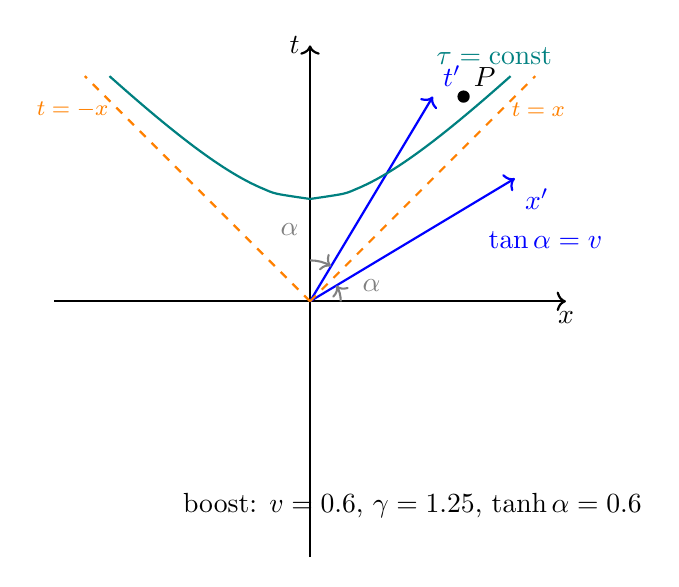
\begin{tikzpicture}[scale=1.3]
    % Original axes (t, x)
    \draw[->,thick] (0,-2.5) -- (0,2.5) node[left] {$t$};
    \draw[->,thick] (-2.5,0) -- (2.5,0) node[below] {$x$};

    % Boosted axes (t', x') - rotated towards light cone
    % t' axis: x = v t, i.e., line with slope 1/v in (t,x) plane
    % For v = 0.6, slope = 1/0.6 ≈ 1.67, angle ≈ 59° from t-axis
    % In (x,t) coordinates on paper: t is vertical, x is horizontal
    % t' axis: t = x/v, so for v=0.6, t = 1.67x
    \draw[->,blue,thick] (0,0) -- (1.2,2.0) node[above right] {$t'$};
    % x' axis: t = vx, so for v=0.6, t = 0.6x
    \draw[->,blue,thick] (0,0) -- (2.0,1.2) node[below right] {$x'$};

    % Light cone lines
    \draw[orange,thick,dashed] (0,0) -- (2.2,2.2) node[pos=0.85,right,font=\footnotesize] {$t=x$};
    \draw[orange,thick,dashed] (0,0) -- (-2.2,2.2) node[pos=0.85,left,font=\footnotesize] {$t=-x$};

    % Angle annotations
    \draw[->,gray] (0.3,0) arc (0:31:0.3);
    \node[gray] at (0.6,0.15) {$\alpha$};
    \draw[->,gray] (0,0.4) arc (90:59:0.4);
    \node[gray] at (-0.2,0.7) {$\alpha$};

    % v=c scaling note
    \node at (1.0, -2.0) {boost: $v = 0.6$, $\gamma = 1.25$, $\tanh\alpha = 0.6$};
    \node[blue] at (2.3, 0.6) {$\tan\alpha = v$};

    % Hyperbola of constant proper time
    \draw[teal,thick,domain=1.0:2.2,smooth,variable=\t] plot ({sqrt(\t*\t-1)},\t);
    \draw[teal,thick,domain=1.0:2.2,smooth,variable=\t] plot ({-sqrt(\t*\t-1)},\t);
    \node[teal] at (1.8, 2.4) {$\tau = \text{const}$};

    % Point P with coordinates in both frames
    \fill (1.5, 2.0) circle (0.06) node[above right] {$P$};
\end{tikzpicture}
\caption{Lorentz boost 的 Minkowski 时空图。黑色轴为原惯性系 $(t, x)$，蓝色轴为以速度 $v = 0.6$ 相对运动的惯性系 $(t', x')$。$t'$ 轴与 $x'$ 轴关于光锥（橙色虚线）对称——它们之间夹角为 $2\alpha$，其中 $\tanh\alpha = v$。青色曲线代表固有时间 $\tau$ 为常数的双曲线——所有惯性系中具有相同固有时间的事件位于同一条双曲线上。}
\label{fig:lorentz_boost}
\end{figure}

\section{四维矢量与张量}

狭义相对论中的物理量自然组织为 Minkowski 时空上的四维张量。三维空间中的矢量（如速度、动量）只是四维对应量的空间分量——它们在不同惯性系下混合。

\subsection{四速度与四动量}

\begin{definition}[四速度]
粒子的\textbf{四速度} (4-velocity) 定义为世界线对固有时间的导数：
\begin{equation}
    u^\mu = \frac{\dd x^\mu}{\dd\tau}.
\end{equation}
由 $\dd\tau^2 = -\eta_{\mu\nu}\dd x^\mu\dd x^\nu$，四速度自动满足归一化条件：
\begin{equation}\label{eq:u_normalization}
    \eta_{\mu\nu} u^\mu u^\nu = -1.
\end{equation}
\end{definition}

在惯性系中，粒子的三维速度为 $\mathbf{v} = \dd\mathbf{x}/\dd t$，则：
\begin{equation}\label{eq:4velocity_components}
    \boxed{u^\mu = \gamma\,(1, \mathbf{v})}, \qquad u_\mu = \eta_{\mu\nu} u^\nu = \gamma\,(-1, \mathbf{v}),
\end{equation}
其中 $\gamma = 1/\sqrt{1 - v^2}$。可以验证 $u^\mu u_\mu = \gamma^2(-1 + v^2) = -1$。

\begin{definition}[四动量]
质量为 $m$ 的粒子的\textbf{四动量} (4-momentum) 为：
\begin{equation}
    p^\mu = m u^\mu = (E, \mathbf{p}),
\end{equation}
其中 $E = \gamma m$ 是相对论能量，$\mathbf{p} = \gamma m \mathbf{v}$ 是相对论动量。
\end{definition}

\begin{property}[质壳条件]
四动量的模方给出著名的 Einstein 能量-动量关系：
\begin{equation}\label{eq:mass_shell}
    \boxed{p^\mu p_\mu = -E^2 + \mathbf{p}^2 = -m^2}.
\end{equation}
这是一个 Lorentz 不变量——在所有惯性系中，$E^2 - \mathbf{p}^2 = m^2$ 恒成立。此关系定义了动量空间中的\textbf{质壳} (mass shell)。
\end{property}

\begin{example}[四速度分量的计算]
考虑一个以速度 $v = 0.6$ 沿 $x$ 轴运动的粒子。计算其四速度分量。
\[
\gamma = \frac{1}{\sqrt{1 - 0.36}} = \frac{1}{0.8} = 1.25.
\]
因此：
\[
u^\mu = \gamma(1, v, 0, 0) = (1.25,\, 0.75,\, 0,\, 0).
\]
验证归一化：$u^\mu u_\mu = -(1.25)^2 + (0.75)^2 = -1.5625 + 0.5625 = -1$。\hfill $\checkmark$

四动量为 $p^\mu = m u^\mu$。在 $v \ll 1$ 的低速极限下：
\[
E = \gamma m = \frac{m}{\sqrt{1 - v^2}} \approx m\Bigl(1 + \frac{v^2}{2}\Bigr) = m + \frac{1}{2}mv^2,
\]
即静止能量 $m$ 加上牛顿动能 $\frac{1}{2}mv^2$。这正是 Einstein 质能关系的根源。
\end{example}

\subsection{四加速度与四力}

\begin{definition}[四加速度]
\textbf{四加速度} (4-acceleration) 是四速度对固有时间的协变导数。在 Minkowski 时空（$\Gamma^\lambda_{\mu\nu} = 0$）中，即普通导数：
\begin{equation}
    a^\mu = \frac{\dd u^\mu}{\dd\tau} = \frac{\dd^2 x^\mu}{\dd\tau^2}.
\end{equation}
由 $u^\mu u_\mu = -1$ 求导得 $a^\mu u_\mu = 0$——四加速度总是与四速度正交。
\end{definition}

\begin{definition}[四力]
\textbf{四力} (4-force) 或 Minkowski 力定义为：
\begin{equation}
    f^\mu = \frac{\dd p^\mu}{\dd\tau} = m a^\mu.
\end{equation}
其空间分量与三维力 $\mathbf{F} = \dd\mathbf{p}/\dd t$ 的关系为 $f^i = \gamma F^i$，时间分量 $f^0 = \gamma\,\mathbf{F}\cdot\mathbf{v}$（即功率）。
\end{definition}

\section{能量--动量张量}

在狭义相对论中，连续介质（流体、场）的能量、动量和应力分布被统一编码在\textbf{能量--动量张量} $T^{\mu\nu}$（也称应力--能量张量）中。

\subsection{完美流体}

\begin{definition}[完美流体的能量--动量张量]
\textbf{完美流体} (perfect fluid) 是理想化的连续介质，在其静止系中无黏滞性和热传导。其能量--动量张量为：
\begin{equation}\label{eq:perfect_fluid}
    \boxed{T^{\mu\nu} = (\rho + p)\,u^\mu u^\nu + p\,\eta^{\mu\nu}},
\end{equation}
其中：
\begin{itemize}
    \item $\rho$ —— 随动系中的\textbf{能量密度} (energy density)；
    \item $p$ —— 随动系中的\textbf{压强} (pressure)；
    \item $u^\mu$ —— 流体元的四速度场。
\end{itemize}
在流体的静止系中（$u^\mu = (1, \mathbf{0})$），能量--动量张量取对角形式：
\begin{equation}
    T^{\mu\nu} = \begin{pmatrix}
        \rho & 0 & 0 & 0 \\
        0 & p & 0 & 0 \\
        0 & 0 & p & 0 \\
        0 & 0 & 0 & p
    \end{pmatrix}.
\end{equation}
\end{definition}

\begin{note}[$T^{\mu\nu}$ 各分量的物理解释]
在一般惯性系中，$T^{\mu\nu}$ 的分量具有清晰的物理含义：
\begin{itemize}
    \item $T^{00}$：能量密度（单位体积内的能量）；
    \item $T^{0i} = T^{i0}$：动量密度 / 能量流密度（第 $i$ 方向单位面积、单位时间内流过的能量）；
    \item $T^{ij}$：应力张量——第 $i$ 方向单位面积上作用的第 $j$ 方向力。对角元 $T^{ii}$（无求和）是正应力（压强），非对角元 $T^{ij}$ ($i\neq j$) 是切应力。
\end{itemize}
\end{note}

\subsection{能量--动量守恒}

在平直时空中，能量--动量守恒表现为能量--动量张量的四维散度为零：
\begin{equation}\label{eq:conservation}
    \boxed{\partial_\mu T^{\mu\nu} = 0}.
\end{equation}
这实际上包含了四个守恒方程：
\begin{itemize}
    \item $\nu = 0$：能量守恒 $\partial_t T^{00} + \partial_i T^{i0} = 0$；
    \item $\nu = i$：动量守恒 $\partial_t T^{0i} + \partial_j T^{ji} = 0$。
\end{itemize}

对于完美流体，代入 (\ref{eq:perfect_fluid}) 后，守恒方程 $\partial_\mu T^{\mu\nu} = 0$ 投影为：
\begin{equation}
    u^\nu \partial_\nu \rho + (\rho + p)\partial_\nu u^\nu = 0 \quad\text{(能量守恒，沿流线)},
\end{equation}
\begin{equation}
    (\rho + p) u^\nu \partial_\nu u^\mu = -(\eta^{\mu\nu} + u^\mu u^\nu)\,\partial_\nu p \quad\text{(相对论 Euler 方程)}.
\end{equation}

\subsection{尘埃与辐射}

\begin{definition}[尘埃]
\textbf{尘埃} (dust) 是压强可以忽略的完美流体（$p=0$）：
\begin{equation}
    T^{\mu\nu}_{\text{dust}} = \rho\, u^\mu u^\nu.
\end{equation}
尘埃描述无相互作用的粒子集合（如宇宙学中的冷暗物质）。尘埃的每个流体元沿测地线运动：
\begin{equation}
    u^\nu \partial_\nu (\rho u^\mu) = 0.
\end{equation}
\end{definition}

\begin{definition}[辐射]
\textbf{辐射} (radiation) 或极端相对论流体对应无质量粒子气体，其状态方程为 $p = \rho/3$。能量--动量张量为：
\begin{equation}
    T^{\mu\nu}_{\text{rad}} = \frac{4}{3}\rho\,u^\mu u^\nu + \frac{1}{3}\rho\,\eta^{\mu\nu},
\end{equation}
且满足无迹条件 $T^\mu{}_\mu = 0$。这是电磁辐射和极端相对论粒子气体的基本特征。
\end{definition}

\section{Maxwell 方程的协变形式}

Maxwell 的电动力学是狭义相对论的最早成功应用。本节用四维张量语言重新表述电磁理论，展示其内蕴的 Lorentz 协变性。

\subsection{四维势与场强张量}

\begin{definition}[电磁四维势]
\textbf{电磁四维势} (electromagnetic 4-potential) $A_\mu$ 将标量势 $\phi$ 和矢量势 $\mathbf{A}$ 统一为：
\begin{equation}
    A_\mu = (-\phi, \mathbf{A}), \qquad A^\mu = \eta^{\mu\nu}A_\nu = (\phi, \mathbf{A}).
\end{equation}
\end{definition}

\begin{definition}[电磁场强张量]
\textbf{电磁场强张量} (field strength tensor) $F_{\mu\nu}$ 定义为四维势的外导数：
\begin{equation}\label{eq:F_definition}
    \boxed{F_{\mu\nu} = \partial_\mu A_\nu - \partial_\nu A_\mu}.
\end{equation}
$F_{\mu\nu}$ 是反对称的 $(0,2)$ 型张量：$F_{\mu\nu} = -F_{\nu\mu}$。其分量与电场 $\mathbf{E}$ 和磁场 $\mathbf{B}$ 的关系为：
\begin{equation}\label{eq:F_components}
    F_{\mu\nu} = \begin{pmatrix}
        0 & -E_x & -E_y & -E_z \\
        E_x & 0 & B_z & -B_y \\
        E_y & -B_z & 0 & B_x \\
        E_z & B_y & -B_x & 0
    \end{pmatrix}, \qquad
    F^{\mu\nu} = \begin{pmatrix}
        0 & E_x & E_y & E_z \\
        -E_x & 0 & B_z & -B_y \\
        -E_y & -B_z & 0 & B_x \\
        -E_z & B_y & -B_x & 0
    \end{pmatrix}.
\end{equation}
\end{definition}

\begin{note}[规范不变性]
四维势 $A_\mu$ 不是唯一的。规范变换 $A_\mu \to A_\mu + \partial_\mu \Lambda$（对任意标量函数 $\Lambda$）不改变场强张量：$F_{\mu\nu} \to F_{\mu\nu}$。这是 $U(1)$ 规范对称性的表现。
\end{note}

\subsection{Maxwell 方程的协变形式}

在四维张量语言中，四个 Maxwell 方程被紧凑地表述为两个张量方程。

\begin{theorem}[Maxwell 方程 —— 协变形式]
有源 Maxwell 方程（Gauss 定律和 Ampère 定律）统一为：
\begin{equation}\label{eq:maxwell_source}
    \boxed{\partial_\mu F^{\mu\nu} = J^\nu},
\end{equation}
其中 $J^\nu = (\rho_e, \mathbf{J})$ 是\textbf{四维电流密度}（$\rho_e$ 为电荷密度，$\mathbf{J}$ 为三维电流密度）。此处已取单位制使 $\mu_0 = \varepsilon_0 = 1$。

无源 Maxwell 方程（Gauss 磁定律和 Faraday 定律）统一为\textbf{Bianchi 恒等式}：
\begin{equation}\label{eq:maxwell_bianchi}
    \boxed{\partial_{[\mu} F_{\nu\rho]} = 0},
\end{equation}
即 $\partial_\mu F_{\nu\rho} + \partial_\nu F_{\rho\mu} + \partial_\rho F_{\mu\nu} = 0$。这是场强张量由四维势定义的自动推论（等价于 $\dd F = 0$，其中 $F = \frac{1}{2}F_{\mu\nu}\dd x^\mu \wedge \dd x^\nu$）。
\end{theorem}

\begin{example}[验证 Maxwell 方程的 Lorentz 协变性]
我们显式验证方程 (\ref{eq:maxwell_source}) 和 (\ref{eq:maxwell_bianchi}) 在 Lorentz 变换下保持形式不变。

设 Lorentz 变换 $x'^\mu = \Lambda^\mu{}_\nu x^\nu$。张量分量的变换规则为：
\[
F'^{\mu\nu} = \Lambda^\mu{}_\rho \Lambda^\nu{}_\sigma F^{\rho\sigma}, \qquad
J'^\nu = \Lambda^\nu{}_\rho J^\rho.
\]
偏导数的变换为 $\partial'_\mu = (\Lambda^{-1})^\nu{}_\mu \partial_\nu$。在 Lorentz 变换下：
\[
\partial'_\mu F'^{\mu\nu} = (\Lambda^{-1})^\alpha{}_\mu \partial_\alpha (\Lambda^\mu{}_\rho \Lambda^\nu{}_\sigma F^{\rho\sigma})
= \Lambda^\nu{}_\sigma (\Lambda^{-1})^\alpha{}_\mu \Lambda^\mu{}_\rho \,\partial_\alpha F^{\rho\sigma}
= \Lambda^\nu{}_\sigma \,\partial_\rho F^{\rho\sigma} = \Lambda^\nu{}_\sigma J^\sigma = J'^\nu.
\]
因此 $\partial_\mu F^{\mu\nu} = J^\nu$ 在 Lorentz 变换下保持形式不变——它是张量方程。同样的推理适用于 $\partial_{[\mu}F_{\nu\rho]} = 0$。\hfill $\square$
\end{example}

\subsection{Lorentz 力的协变形式}

\begin{theorem}[Lorentz 力 —— 协变形式]
电荷为 $q$ 的带电粒子在电磁场中受到的\textbf{Lorentz 四力}为：
\begin{equation}\label{eq:lorentz_force}
    \boxed{f^\mu = q\,F^{\mu\nu} u_\nu},
\end{equation}
其中 $u^\nu$ 是粒子的四速度。此方程同时包含了三维 Lorentz 力 $\mathbf{F} = q(\mathbf{E} + \mathbf{v}\times\mathbf{B})$ 和功率方程 $\dd E/\dd t = q\mathbf{E}\cdot\mathbf{v}$。
\end{theorem}

\begin{proof}[Lorentz 力的分量展开]
展开 $f^\mu = q F^{\mu\nu}u_\nu$。对于 $\mu = i$（空间分量）：
\[
f^i = q(F^{i0}u_0 + F^{ij}u_j) = q\bigl(E^i \cdot (-\gamma) + \varepsilon^{ijk}B_k \cdot (\gamma v^j)\bigr)
= q\gamma\,(E^i + (\mathbf{v}\times\mathbf{B})^i).
\]
由于 $f^i = \gamma F^i$，得 $F^i = q(E^i + (\mathbf{v}\times\mathbf{B})^i)$——即三维 Lorentz 力。

对于 $\mu = 0$（时间分量）：
\[
f^0 = q F^{0j}u_j = q E^j \cdot (\gamma v^j) = q\gamma\,\mathbf{E}\cdot\mathbf{v}.
\]
由于 $f^0 = \gamma\,\dd E/\dd t$，得 $\dd E/\dd t = q\mathbf{E}\cdot\mathbf{v}$——即电磁场对带电粒子做功的功率。
\end{proof}

\subsection{能量--动量张量的电磁对应物}

电磁场本身携带着能量和动量。电磁场的能量--动量张量为：
\begin{equation}\label{eq:em_stress_energy}
    T^{\mu\nu}_{\text{EM}} = F^{\mu\rho} F^\nu{}_\rho - \frac{1}{4}\eta^{\mu\nu} F_{\rho\sigma}F^{\rho\sigma}.
\end{equation}
其分量与电磁场的能量密度 $u = \frac{1}{2}(\mathbf{E}^2 + \mathbf{B}^2)$、Poynting 矢量 $\mathbf{S} = \mathbf{E}\times\mathbf{B}$ 以及 Maxwell 应力张量的关系为：
\begin{equation}
    T^{00}_{\text{EM}} = \frac{1}{2}(\mathbf{E}^2 + \mathbf{B}^2), \quad
    T^{0i}_{\text{EM}} = (\mathbf{E}\times\mathbf{B})^i, \quad
    T^{ij}_{\text{EM}} = -E^i E^j - B^i B^j + \frac{1}{2}\delta^{ij}(\mathbf{E}^2 + \mathbf{B}^2).
\end{equation}
可以验证 $\partial_\mu T^{\mu\nu}_{\text{EM}} = -F^{\nu\rho}J_\rho$——电磁场的能量--动量不是独立守恒的，而是与带电物质交换能量和动量。

\subsection{不变量与对偶}

\begin{example}[电磁场的不变量：$\mathbf{E}^2 - \mathbf{B}^2$ 和 $\mathbf{E}\cdot\mathbf{B}$]
电磁场有两个独立的 Lorentz 不变量：
\[
F_{\mu\nu}F^{\mu\nu} = 2(\mathbf{B}^2 - \mathbf{E}^2), \qquad
\tilde{F}_{\mu\nu}F^{\mu\nu} = -4\,\mathbf{E}\cdot\mathbf{B},
\]
其中 $\tilde{F}_{\mu\nu} = \frac{1}{2}\varepsilon_{\mu\nu\rho\sigma}F^{\rho\sigma}$ 是 Hodge 对偶场强（$\varepsilon_{0123} = 1$）。

这两个不变量的物理意义：
\begin{itemize}
    \item 若 $\mathbf{B}^2 > \mathbf{E}^2$（磁场主导），则存在惯性系使得电场为零；
    \item 若 $\mathbf{E}^2 > \mathbf{B}^2$（电场主导），则存在惯性系使得磁场为零；
    \item 若 $\mathbf{E}\cdot\mathbf{B} \neq 0$，则电磁场具有手性（如在电磁波中 $\mathbf{E}\cdot\mathbf{B} = 0$，即电场与磁场正交）；
    \item 平面电磁波满足 $F_{\mu\nu}F^{\mu\nu} = 0$ 和 $\tilde{F}_{\mu\nu}F^{\mu\nu} = 0$——两个不变量同时为零。
\end{itemize}
\end{example}

\section{从狭义相对论到广义相对论}

经过以上各节的回顾，我们现在处于一个关键的分水岭：我们已经在 Minkowski 平直时空中建立了完整的相对论物理学框架。但狭义相对论有一个根本性的局限——它无法容纳引力。

\subsection{狭义相对论的局限}

\begin{remark}[狭义相对论为何不能描述引力]
狭义相对论在以下方面与引力不相容：
\begin{enumerate}
    \item \textbf{引力的普适性与惯性系的优先地位}：狭义相对论赋予惯性系以特殊地位，但引力的普适性（所有物体同样下落）表明，引力场中的\textbf{自由下落参考系}才是真正的\"惯性系\"——而这正是非惯性系。
    \item \textbf{引力的潮汐效应}：两个相邻自由下落粒子之间的相对加速度（潮汐力）无法在平直时空的框架内描述，因为零曲率意味着相邻测地线永远平行——但实际引力场中它们会汇聚或发散。
    \item \textbf{光在引力场中的偏折}：狭义相对论预言光沿直线传播（类光测地线在平直时空中是直线），但实际观测（1919年日食观测）证实了星光经过太阳附近时发生偏折。
    \item \textbf{牛顿引力的瞬时传播}：牛顿引力是超距作用，违反狭义相对论的光速极限。任何相对论性的引力理论必须以有限速度传播。
    \item \textbf{等效原理}：惯性质量与引力质量的精确相等（Eötvös 实验精度已达 $10^{-15}$）是一个深刻的谜团，暗示引力与惯性之间存在本质联系——这种联系在平直时空的框架内无法自然解释。
\end{enumerate}
\end{remark}

\subsection{Einstein 的洞察：引力 = 时空弯曲}

\begin{note}[从平直时空到弯曲时空的关键跃迁]
Einstein 的洞见可以概括为三个递进的层次：
\begin{enumerate}
    \item \textbf{等效原理}：在局部范围内，引力和加速度不可区分。这意味着自由下落参考系中的物理定律与狭义相对论中的形式相同——在时空的每个点上，存在一个局部惯性系，其中度规取 Minkowski 形式 $\eta_{\mu\nu}$ 且 Christoffel 符号为零。
    \item \textbf{引力的几何化}：既然局部惯性系因时空点而异（不同点的自由下落参考系彼此有相对加速度），唯一的可能是时空本身是弯曲的。引力不再是一种\"力\"，而是时空弯曲的表现。
    \item \textbf{度规作为引力势}：Minkowski 度规 $\eta_{\mu\nu}$ 被推广为一般弯曲时空中的动力学度规场 $g_{\mu\nu}(x)$。在局部惯性系中 $g_{\mu\nu}$ 约化为 $\eta_{\mu\nu}$，但 $g_{\mu\nu}$ 的二阶导数（曲率）体现了真实的引力场——潮汐力。这与牛顿引力势 $\Phi$ 的角色完全平行：$\Phi$ 本身可以通过坐标变换消除（等效原理），但其二阶导数是物理的（潮汐张量）。
\end{enumerate}
\end{note}

\begin{theorem}[最小耦合原理 —— 预览]
从狭义相对论过渡到广义相对论的\"处方\"是\textbf{最小耦合原理} (minimal coupling principle)：
\begin{equation}\label{eq:minimal_coupling}
    \boxed{\eta_{\mu\nu} \;\longrightarrow\; g_{\mu\nu}(x), \qquad \partial_\mu \;\longrightarrow\; \nabla_\mu}.
\end{equation}
即，将平直时空度规替换为弯曲时空度规，将普通导数替换为协变导数。在此规则下，狭义相对论的所有物理定律被\"提升\"为广义相对论中弯曲时空的物理定律。

例如，自由粒子从 $m\,\dd^2 x^\mu / \dd\tau^2 = 0$（平直时空）提升为测地线方程 $\dd^2 x^\mu/\dd\tau^2 + \Gamma^\mu_{\nu\rho} \dot x^\nu \dot x^\rho = 0$（弯曲时空）；能量--动量守恒从 $\partial_\mu T^{\mu\nu} = 0$ 提升为 $\nabla_\mu T^{\mu\nu} = 0$。
\end{theorem}

\begin{note}[本章总结与展望]
本章用微分几何的语言系统回顾了狭义相对论的核心内容：
\begin{itemize}
    \item Minkowski 时空是全局平坦的伪黎曼流形 $(\mathbb{R}^4, \eta)$，光锥定义了因果结构；
    \item Lorentz 变换是保持 $\eta_{\mu\nu}$ 不变的线性变换，构成群 $\mathrm{SO}^+(3,1)$；
    \item 物理量被统一为四维张量——四速度、四动量、能量--动量张量；
    \item Maxwell 方程以 $F_{\mu\nu}$ 的简洁形式展现了其内蕴的 Lorentz 协变性；
    \item 狭义相对论的根本局限在于无法容纳引力，而 Einstein 的解决方案是：\textbf{放弃平直时空，拥抱弯曲时空}。
\end{itemize}

从下一章开始，我们将进入广义相对论的核心：等效原理、广义协变性、爱因斯坦场方程，以及它们如何将\"引力 = 时空弯曲\"这一深刻思想转化为精确的数学理论。
\end{note}

%=============================================================================
% 习题
%=============================================================================

\section*{本章习题}

\begin{enumerate}
    \item 验证快度参数化的 boost 矩阵 (\ref{eq:boost_rapidity}) 满足 Lorentz 条件 $\Lambda^T\eta\Lambda = \eta$。
    \item 从 $E^2 - \mathbf{p}^2 = m^2$ 出发，推导相对论粒子的速度-动量关系 $\mathbf{v} = \mathbf{p}/E$。
    \item 验证电磁场强张量 (\ref{eq:F_definition}) 在规范变换 $A_\mu \to A_\mu + \partial_\mu\Lambda$ 下不变。
    \item 从 $\partial^\mu T^{\text{EM}}_{\mu\nu} = -F_{\nu\rho}J^\rho$ 出发，推导 Poynting 定理（电磁能量守恒）。
    \item 证明平面电磁波满足 $F_{\mu\nu}F^{\mu\nu} = 0$ 和 $\tilde{F}_{\mu\nu}F^{\mu\nu} = 0$。
    \item 利用 Lorentz 变换，证明在一个惯性系中的纯电场，在另一个以速度 $\mathbf{v}$ 相对运动的惯性系中会产生磁场。
\end{enumerate}
  % 狭义相对论回顾
% chapter09.tex - 等效原理与广义协变性
\chapter{等效原理与广义协变性 (Equivalence Principle and General Covariance)}
\label{chap:equivalence}

等效原理是广义相对论最核心的物理基石，广义协变性原理则为理论提供了数学框架。本章系统阐述这两大原理的物理内涵、实验检验和数学表述，并由此自然导出弯曲时空中的物理定律构造方法——最小耦合原理。

\section{引力与加速度的等价性}

\subsection{升降机思想实验}

爱因斯坦在1907年提出了著名的升降机思想实验，深刻揭示了引力与加速度之间的内在联系。考虑两个完全封闭的升降机：

\begin{enumerate}
    \item \textbf{升降机 A}：静止在地球表面，感受到向下的均匀引力场 $\vb*{g} = -g \vu*{z}$。
    \item \textbf{升降机 B}：在无引力的空无一物的空间中，以恒定加速度 $\vb*{a} = +g \vu*{z}$ 向上加速。
\end{enumerate}

\begin{figure}[htbp]
\centering
\begin{tikzpicture}[scale=1.1]
    % --- 升降机 A：地球引力 ---
    \draw[thick] (-2.5, -1.5) rectangle (0.5, 2.0);
    \node at (-1.0, 1.7) {升降机 A};
    % 内部的人
    \fill (-1.0, 0.3) circle (0.15);
    \draw (-1.0, 0.3) -- (-1.0, -0.3);
    \draw (-1.0, -0.3) -- (-1.2, -0.8);
    \draw (-1.0, -0.3) -- (-0.8, -0.8);
    % 掉落的苹果
    \fill[red] (-0.5, 1.2) circle (0.08);
    \draw[red, ->, thick] (-0.5, 1.2) -- (-0.5, 0.5);
    \node[red, right] at (-0.5, 0.8) {苹果下落};
    % 地球
    \shade[ball color=brown!40] (-4.0, -3.0) circle (0.8);
    \draw[->, thick] (-1.0, -1.5) -- (-1.0, -1.9);
    \node at (-1.0, -2.15) {$\vb*{g}$ 向下};
    % 标签
    \node at (-1.0, -2.6) {引力场中静止};

    % --- 升降机 B：加速参考系 ---
    \begin{scope}[xshift=4.5cm]
    \draw[thick] (-2.5, -1.5) rectangle (0.5, 2.0);
    \node at (-1.0, 1.7) {升降机 B};
    % 内部的人（漂浮）
    \fill (-1.0, 0.3) circle (0.15);
    \draw (-1.0, 0.3) -- (-1.0, -0.3);
    \draw (-1.0, -0.3) -- (-1.2, -0.8);
    \draw (-1.0, -0.3) -- (-0.8, -0.8);
    % 苹果相对人"下落"
    \fill[red] (-0.5, 1.2) circle (0.08);
    \draw[red, ->, thick] (-0.5, 1.2) -- (-0.5, 0.5);
    \node[red, right] at (-0.5, 0.8) {苹果"下落"};
    % 加速箭头
    \draw[->, thick] (-1.0, -1.5) -- (-1.0, -1.9);
    \node at (-1.0, -2.15) {$\vb*{a}$ 向上};
    \node[blue] at (-1.0, -2.7) {加速上升};
    % 虚线表示无引力空间
    \draw[blue, dashed] (-0.2, -3.3) -- (3.2, -3.3);
    \node[blue] at (1.5, -3.5) {无引力真空};
    \end{scope}

    % 等号
    \node at (2.0, 0.25) {\Huge $\Longleftrightarrow$};
    \node at (2.0, -0.4) {不可分辨};

\end{tikzpicture}
\caption{升降机思想实验。升降机A静止在引力场中，苹果因引力下落；升降机B在无引力空间中加速上升，苹果因惯性而相对于加速参考系"下落"。封闭在升降机内的观察者无法通过任何局部力学实验区分这两种情况。}
\label{fig:elevator}
\end{figure}

\textbf{关键结论：}封闭在升降机内部的观察者无法通过任何局部实验来判断自己处于引力场中还是处于加速参考系中。这一观察可以精确表述为：

\begin{definition}[弱等效原理 (Weak Equivalence Principle, WEP)]
在引力场中，所有检验物体的运动轨迹仅取决于其初始位置和速度，而与物体的质量和内部组成无关。等价的数学表述为：引力质量 $m_G$ 与惯性质量 $m_I$ 相等，
\begin{equation}
    m_I = m_G .
\end{equation}
\label{def:WEP}
\end{definition}

\subsection{E\"{o}tv\"{o}s 实验与现代检验}

弱等效原理的实验基础可以追溯到伽利略的比萨斜塔思想实验和牛顿的单摆实验，但系统性的精密检验始于E\"{o}tv\"{o}s。

\begin{example}[E\"{o}tv\"{o}s 扭摆实验，1890--1922]
E\"{o}tv\"{o}s 扭摆实验的原理如下：将两个不同材料（如木和铂）的物体悬挂在扭摆的两端。若 $m_G/m_I$ 因材料而异，则地球自转产生的离心力与引力的合力方向将随材料变化，从而在扭摆上产生净扭矩。设地球引力加速度为 $\vb*{g}$，自转离心加速度为 $\vb*{a}_c = \omega^2 R_\oplus \sin\theta \, \vu*{e}_\perp$，则悬挂方向由下式决定：
\begin{equation}
    \tan\alpha = \frac{m_I}{m_G} \frac{a_c}{g}.
\end{equation}
若 $m_I/m_G$ 依赖于材料成分，则 $\alpha$ 随材料变化，扭摆会转动。E\"{o}tv\"{o}s 得到
\begin{equation}
    \left|\frac{m_G}{m_I} - 1\right| < 5 \times 10^{-9}.
\end{equation}
\end{example}

现代实验已将这一精度推向极致：

\begin{itemize}
    \item \textbf{E\"{o}t-Wash 实验}（华盛顿大学，1990--2008）：利用改进的扭摆技术，达到
    \begin{equation}
        \left|\frac{m_G}{m_I} - 1\right| < 10^{-13}.
    \end{equation}
    \item \textbf{MICROSCOPE 卫星}（法国，2016--2022）：在太空微重力环境中进行，精度达到
    \begin{equation}
        \eta = \frac{2(m_G/m_I)_A - 2(m_G/m_I)_B}{(m_G/m_I)_A + (m_G/m_I)_B} < 2.7 \times 10^{-15}.
    \end{equation}
    \item \textbf{月球激光测距}（LLR）：通过精确测量月球轨道，检验了地球和月球的 $m_G/m_I$ 等价性，精度约 $10^{-13}$。
\end{itemize}

这些实验使弱等效原理成为物理学中最精确检验的原理之一。

\subsection{等效原理的三层表述}

等效原理并非单一陈述，而是从弱到强的三层嵌套表述：

\begin{definition}[弱等效原理 (WEP)]
引力质量等于惯性质量，检验粒子在引力场中的运动与组成无关。
\end{definition}

\begin{definition}[爱因斯坦等效原理 (Einstein Equivalence Principle, EEP)]
WEP 加上以下两个条件：
\begin{enumerate}
    \item \textbf{局部 Lorentz 不变性 (LLI)}：在任何局部自由下落参考系中，非引力的物理实验结果与参考系的速度（方向和大小）无关。
    \item \textbf{局部位置不变性 (LPI)}：在任何局部自由下落参考系中，非引力的物理实验结果与实验在时空中的位置和时间无关。
\end{enumerate}
简言之，在局部自由下落参考系中，狭义相对论（以及整个非引力的标准模型物理）成立。
\end{definition}

\begin{definition}[强等效原理 (Strong Equivalence Principle, SEP)]
EEP 再加一个条件：引力自身能量的 $m_G/m_I$ 比值也等于1。换言之，\textbf{所有物理定律}——包括引力定律本身——在局部自由下落参考系中取其在狭义相对论中的形式。这意味着引力的自能量（self-energy）不产生异常的惯性或引力效应。
\end{definition}

\begin{note}[SEP 与 WEP/EEP 的区别]
广义相对论满足 EEP，但是否满足 SEP 取决于具体情况。在纯广义相对论中（无标量场等），SEP 成立。但在许多修正引力理论（如标量-张量理论）中，引力自能的 $m_G/m_I$ 可能偏离1，导致 SEP 破缺。因此 SEP 的检验可以区分广义相对论与其他引力理论。
\end{note}

\begin{table}[htbp]
\centering
\caption{等效原理的三层表述及其检验}
\begin{tabular}{p{2.5cm} p{5cm} p{5cm}}
\toprule
\textbf{原理} & \textbf{核心内容} & \textbf{检验实验} \\
\midrule
WEP & $m_I=m_G$，运动轨迹与组成无关 & E\"{o}tv\"{o}s, E\"{o}t-Wash, MICROSCOPE \\
EEP & 局部物理定律与SR一致 & 引力红移 (Pound-Rebka)、Hughes-Drever实验 \\
SEP & 引力自能量也满足 $m_I=m_G$ & 月球激光测距（Nordtvedt效应）、脉冲星双星 \\
\bottomrule
\end{tabular}
\label{tab:ep_levels}
\end{table}

\section{引力时间膨胀的推导}

\subsection{从加速参考系的多普勒频移到引力红移}

等效原理最深刻的推论之一是引力场中的时间膨胀效应。我们可以通过加速参考系中的多普勒频移来推导。

\textbf{步骤一：加速参考系中的频移。} 考虑一个在无引力空间中沿 $z$ 轴以恒定加速度 $a$ 加速的火箭。在火箭的瞬时静止参考系中，等效原理告诉我们它与均匀引力场中的静止参考系不可区分。设在火箭底部（$z=0$）有一个光源，顶部（$z=h$）有一个探测器。

在 $t=0$ 时刻，底部光源发出一个频率为 $\nu_0$ 的光信号。此时火箭的瞬时速度为0。光信号以速度 $c$ 向上传播，到达顶部的时间为 $\Delta t \approx h/c$。在这段时间内，火箭获得的速度增量为
\begin{equation}
    \Delta v = a \Delta t = \frac{a h}{c}.
\end{equation}
由于多普勒效应，顶部探测器接收到的频率为（对 $v \ll c$ 的非相对论情况）：
\begin{equation}
    \nu_{\text{rec}} = \nu_0 \left(1 - \frac{\Delta v}{c}\right) = \nu_0 \left(1 - \frac{ah}{c^2}\right).
\end{equation}

\textbf{步骤二：等效原理翻译为引力红移。} 根据等效原理，加速参考系中的物理等效于均匀引力场中的物理。将加速度 $a$ 替换为引力加速度 $g$（即单位质量所受引力 $g = GM/r^2$），得到：
\begin{equation}
    \frac{\nu_{\text{rec}} - \nu_0}{\nu_0} = -\frac{g h}{c^2}.
\end{equation}
这意味着在引力场中，从低引力势向高引力势传播的光会发生红移。

\begin{theorem}[引力红移公式——弱场近似]
在弱静态引力场中，设 $\Phi(\vb*{x})$ 为牛顿引力势（满足 $\nabla^2 \Phi = 4\pi G \rho$），频率变化为
\begin{equation}
    \boxed{\frac{\Delta\nu}{\nu} = \frac{\Phi_{\text{em}} - \Phi_{\text{obs}}}{c^2}}.
\end{equation}
等价地，坐标时与固有时的关系为
\begin{equation}
    \dd\tau = \sqrt{1 + \frac{2\Phi}{c^2}} \, \dd t \approx \left(1 + \frac{\Phi}{c^2}\right) \dd t.
\end{equation}
\end{theorem}

\begin{proof}[加速参考系推导的严格版本]
设火箭底部光源发射光信号的时刻为 $t_1$（火箭瞬时静止），顶部探测器接收到信号的时刻为 $t_2$。在 Rindler 坐标系中，火箭底部的固有时 $d\tau_{\text{bottom}}$ 与顶部的固有时 $d\tau_{\text{top}}$ 的关系为
\begin{equation}
    d\tau_{\text{top}} = \left(1 + \frac{ah}{c^2}\right) d\tau_{\text{bottom}}.
\end{equation}
将 $a \to g$ 翻译为引力场，即得 $d\tau_{\text{top}}/d\tau_{\text{bottom}} = 1 + gh/c^2$。对于地球表面，
\begin{equation}
    \frac{gh}{c^2} \approx \frac{9.8 \times 10}{9 \times 10^{16}} \approx 1.1 \times 10^{-15}.
\end{equation}
这是一个极小的效应，但可以被精密测量所检测。
\end{proof}

\subsection{Pound--Rebka 实验 (1960)}

\begin{example}[Pound--Rebka 实验]
1960年，Pound 和 Rebka 在哈佛大学 Jefferson 实验室的塔楼中（高度差 $h=22.5\,\text{m}$）利用 M\"{o}ssbauer 效应测量了引力红移。$^{57}\text{Fe}$ 的 14.4 keV $\gamma$ 射线具有极窄的线宽（$\Delta\nu/\nu \approx 10^{-12}$），使如此微小的频移可被检测。

理论预测的频移为
\begin{equation}
    \frac{\Delta\nu}{\nu} = \frac{gh}{c^2} = \frac{9.8 \times 22.5}{9 \times 10^{16}} \approx 2.46 \times 10^{-15}.
\end{equation}
实验结果与理论预测的偏差在 $10\%$ 以内，后经 Pound--Snider (1964) 改进至 $1\%$。

1976年的 \textbf{Gravity Probe A} 实验将氢钟搭载到 $10^4\,\text{km}$ 高度，以 $7\times 10^{-5}$ 的精度验证了引力红移公式。2018年的 \textbf{GALILEO 5/6 卫星}（因发射故障进入椭圆轨道）提供了 $10^{-4}$ 精度的额外检验。
\end{example}

\section{光线偏折的等效原理推导}

\subsection{等效原理预言光线偏折}

等效原理不仅能推导引力红移，还能预言光线在引力场中的偏折。虽然等效原理给出的偏折角恰好是广义相对论精确值的一半，但这个推导极具教学意义——它清晰地展示了等效原理的适用范围和局限。

\begin{example}[用等效原理推导光线偏折——因子2错误]
考虑一束光从远处掠过太阳表面。在太阳附近，引力场可近似为均匀的。设光子在太阳引力场中沿 $x$ 方向传播，引力沿 $z$ 方向。

\textbf{等效原理推理：} 在自由下落参考系中，光子沿直线传播。从地球（远离太阳的惯性系）看来，太阳附近的时空可以看作一个"加速向下"的区域。光子穿越这一区域的时间约为 $\Delta t \approx 2R_\odot / c$（直径穿越），在此期间光子获得的横向速度增量为
\begin{equation}
    \Delta v_z = g \Delta t = \frac{GM_\odot}{R_\odot^2} \cdot \frac{2R_\odot}{c} = \frac{2GM_\odot}{c R_\odot}.
\end{equation}
因此偏折角为（小角度近似）
\begin{equation}
    \boxed{\Delta\theta_{\text{EP}} = \frac{\Delta v_z}{c} = \frac{2GM_\odot}{c^2 R_\odot}}.
\end{equation}
代入太阳数据：$G = 6.674 \times 10^{-11}\,\text{m}^3\text{kg}^{-1}\text{s}^{-2}$, $M_\odot = 1.989 \times 10^{30}\,\text{kg}$, $R_\odot = 6.957 \times 10^8\,\text{m}$, $c = 2.998 \times 10^8\,\text{m/s}$，
\begin{equation}
    \Delta\theta_{\text{EP}} \approx 0.875'' \;\;(\text{角秒}).
\end{equation}
\end{example}

\begin{note}[因子2的缺失]
广义相对论给出的精确偏折角是 \textbf{两倍}于等效原理的预言：
\begin{equation}
    \boxed{\Delta\theta_{\text{GR}} = \frac{4GM_\odot}{c^2 R_\odot} \approx 1.75''}.
\end{equation}
等效原理漏掉的因子2来源于空间弯曲的贡献。等效原理只考虑了"时间弯曲"（$g_{00}$ 分量）——即引力时间膨胀对光速的影响，而没有计入空间弯曲（$g_{ij}$ 分量）对光传播路径的额外偏折。在广义相对论中，时间弯曲和空间弯曲各贡献 $\Delta\theta/2 = 0.875''$。这一事实说明：\textbf{等效原理在局部成立，但光线偏折是一个非局部的、整体的效应，需要完整的时空弯曲描述。}
\end{note}

\subsection{Eddington 日食观测 (1919) 与后续检验}

\begin{example}[Eddington 日食观测]
1919年5月29日，Arthur Eddington 率领两支远征队分别前往巴西的 Sobral 和西非的 Pr\'{i}ncipe 岛观测日全食。通过比较日食期间和夜晚拍摄的星场照片，测量星光掠过太阳边缘时的偏折角。结果：
\begin{equation}
    \Delta\theta_{\text{Sobral}} = 1.98'' \pm 0.16'', \quad
    \Delta\theta_{\text{Pr\'{i}ncipe}} = 1.61'' \pm 0.40''.
\end{equation}
虽然误差较大，但结果明确支持广义相对论（$1.75''$）而非牛顿预言（$0.875''$，等效原理值）。

\textbf{现代射电干涉测量：} 甚长基线干涉测量（VLBI）已将光线偏折的测量精度提升至 $10^{-4}$ 量级，完全确认了广义相对论的 $1.75''$ 预言。
\end{example}

\section{广义协变性原理}

\subsection{数学表述}

广义协变性原理是广义相对论的基本对称性原则：

\begin{definition}[广义协变性原理 (Principle of General Covariance)]
物理定律必须用\textbf{张量方程}表达，使其在任意坐标变换下保持形式不变。具体而言，若物理定律在坐标系 $\{x^\mu\}$ 中写为
\begin{equation}
    T^{\mu_1\cdots\mu_k}_{\nu_1\cdots\nu_\ell} = 0,
\end{equation}
则在任意坐标变换 $x^\mu \to x'^\mu$ 下，它自动变为
\begin{equation}
    T'^{\mu_1\cdots\mu_k}_{\nu_1\cdots\nu_\ell} = 0.
\end{equation}
张量变换保证了这一性质。
\end{definition}

在数学上，广义协变性等价于物理定律在微分同胚群 $\mathrm{Diff}(M)$ 下的协变性。考虑时空流形 $M$ 上的微分同胚 $\phi: M \to M$，张量场的变换为推前 (push-forward) 和拉回 (pull-back)：
\begin{equation}
    (\phi_* T)^{\mu_1\cdots\mu_k}_{\nu_1\cdots\nu_\ell}(p) 
    = \frac{\partial x'^{\mu_1}}{\partial x^{\rho_1}} \cdots 
      \frac{\partial x^{\nu_\ell}}{\partial x'^{\sigma_\ell}} \,
      T^{\rho_1\cdots\rho_k}_{\sigma_1\cdots\sigma_\ell}(\phi^{-1}(p)).
\end{equation}

\begin{note}[主动与被动观点]
广义协变性有两种等价的解读方式：
\begin{itemize}
    \item \textbf{被动微分同胚 (Passive diffeomorphism)}：物理系统不变，只是改变了描述它的坐标系。这相当于同一物理状态的不同坐标表示。
    \item \textbf{主动微分同胚 (Active diffeomorphism)}：坐标系不变，物理系统本身被"拖拽"到了流形上的不同位置。在广义相对论中，主动微分同胚是规范对称性——它将物理上不可区分的构型联系起来。
\end{itemize}
这两种观点的等价性是广义相对论规范结构的核心。
\end{note}

\subsection{Kretschmann 反对与物理解析}

1917年，Erich Kretschmann 提出了著名的反对意见：

\begin{quote}
    \textbf{Kretschmann 反对：} 任何物理理论——包括牛顿力学和狭义相对论——都可以通过引入适当的几何结构而被改写为"广义协变"的形式。因此广义协变性不是一个有物理内容的选择性原则。
\end{quote}

\begin{note}[Kretschmann 反对的解析]
Kretschmann 反对在技术上是正确的：通过足够精巧的数学操作，任何理论都可以写成广义协变的形式（例如，牛顿引力可以用 Newton--Cartan 几何表达）。然而，广义协变性在广义相对论中具有特殊的物理意义：
\begin{enumerate}
    \item \textbf{无背景结构 (No background structure)}：在广义相对论中，度规 $g_{\mu\nu}$ 本身是动力学变量，而牛顿力学和狭义相对论中存在先验的、非动力学的绝对时空结构（如 Minkowski 度规 $\eta_{\mu\nu}$）。
    \item \textbf{等效原理的实现}：广义协变性确保物理定律在局部惯性系中取狭义相对论的形式，这正是等效原理的数学表达。
    \item \textbf{规范对称性}：广义协变性是广义相对论的规范对称性，与之相关的约束方程（Hamiltonian 和 momentum 约束）是理论的动力学核心。
\end{enumerate}
因此，广义协变性的真正物理内容不在于"方程可以写成张量形式"，而在于\textbf{时空的几何结构本身是动力学的}——这是广义相对论与所有前相对论物理的根本区别。Anderson (1967) 和 Friedman (1983) 对这一问题有精辟的分析。
\end{note}

\section{从平直时空到弯曲时空}

\subsection{度规作为动力学场}

在狭义相对论中，时空是刚性、平坦的 Minkowski 时空，度规 $\eta_{\mu\nu} = \mathrm{diag}(-1,1,1,1)$ 是固定的、非动力学的背景。广义相对论的核心变革在于：\textbf{度规 $g_{\mu\nu}(x)$ 成为一个动力学场}——它既描述时空的几何，又描述引力。

\begin{definition}[度规的动力学角色]
在广义相对论中，度规张量 $g_{\mu\nu}(x)$ 扮演双重角色：
\begin{enumerate}
    \item \textbf{几何角色}：定义时空的度量结构——距离、角度、体积。
    \item \textbf{动力学角色}：作为引力场的势，其导数给出"引力场强"（Christoffel 符号），其二阶导数给出"潮汐力"（曲率张量）。
\end{enumerate}
\end{definition}

\begin{figure}[htbp]
\centering
\begin{tikzpicture}[scale=1.2]
    % 弯曲时空背景 (用波浪线暗示)
    \draw[gray!30, line width=2pt] plot[smooth, tension=0.8] coordinates {(-3.5,1.2) (-2.5,0.8) (-1.5,1.5) (-0.5,0.5) (0.5,1.3) (1.5,0.6) (2.5,1.4) (3.5,0.7)};
    \draw[gray!30, line width=2pt] plot[smooth, tension=0.8] coordinates {(-3.5,-0.2) (-2.5,0.3) (-1.5,-0.5) (-0.5,0.1) (0.5,-0.4) (1.5,0.2) (2.5,-0.3) (3.5,0.1)};
    
    % 局部惯性系（放大方框）
    \draw[blue, thick, fill=blue!5] (0.3, -0.2) rectangle (2.0, 1.1);
    \node[blue] at (1.15, 1.35) {局部惯性系 (LIF)};
    
    % 在局部惯性系中画Minkowski坐标网格
    \begin{scope}[shift={(0.5, 0.0)}]
        \draw[blue!60, very thin] (0.0,0.0) grid[step=0.3] (1.2,0.6);
        \draw[blue, ->] (0.6,0.3) -- (0.9,0.3) node[right] {$x$};
        \draw[blue, ->] (0.6,0.3) -- (0.6,0.6) node[above] {$t$};
    \end{scope}
    \node[blue, font=\small] at (1.8, -0.5) {$g_{\mu\nu} = \eta_{\mu\nu} + \mathcal{O}(x^2)$};

    % 自由下落粒子世界线
    \draw[red, thick, ->] (-3.0, -0.5) .. controls (-1.5, -0.8) and (-0.5, 0.8) .. (0.5, 1.0);
    \node[red] at (-1.8, 0.0) {自由下落粒子};
    
    % 全局弯曲时空标注
    \node at (-2.2, 1.6) {弯曲时空};
    \node at (-2.2, 1.2) {$(M, g_{\mu\nu})$};
    
    % 箭头指向局部惯性系
    \draw[->, thick, blue!70] (-1.5, 2.0) .. controls (0.0, 2.3) .. (1.15, 1.5);
    \node[blue] at (-0.5, 2.4) {局部等效于 Minkowski 时空};
    
\end{tikzpicture}
\caption{等效原理的几何表示。在弯曲时空 $(M, g_{\mu\nu})$ 的每一点，存在一个局部惯性系（Local Inertial Frame, LIF），在其中度规退化为 Minkowski 度规 $\eta_{\mu\nu}$ 到一阶精度。自由下落粒子在局部惯性系中沿直线运动，在全局弯曲时空中沿测地线运动。}
\label{fig:lif_curved}
\end{figure}

\subsection{自由运动从直线推广为测地线}

在狭义相对论中，自由粒子的运动方程为
\begin{equation}
    \frac{\dd^2 x^\mu}{\dd\tau^2} = 0,
\end{equation}
即粒子沿 Minkowski 时空中的直线运动。根据等效原理，在弯曲时空中，自由粒子应当沿"尽可能直"的路径运动——这就是\textbf{测地线}：

\begin{equation}
    \boxed{\frac{\dd^2 x^\mu}{\dd\tau^2} + \Gamma^\mu{}_{\nu\rho} \frac{\dd x^\nu}{\dd\tau} \frac{\dd x^\rho}{\dd\tau} = 0}.
\end{equation}

在局部惯性系中（$\Gamma^\mu{}_{\nu\rho} = 0$），测地线方程精确退化为 $\dd^2 x^\mu/\dd\tau^2 = 0$，满足等效原理的要求。

\section{最小耦合原理}

\subsection{原理的精确表述}

最小耦合原理 (Minimal Coupling Principle) 是将狭义相对论中的物理定律推广到弯曲时空的标准方法。

\begin{definition}[最小耦合原理 (Minimal Coupling Principle)]
将狭义相对论中成立的张量形式的物理定律推广到弯曲时空时，做以下替换：
\begin{enumerate}
    \item $\eta_{\mu\nu} \;\longrightarrow\; g_{\mu\nu}$ —— 将 Minkowski 度规替换为弯曲时空度规
    \item $\partial_\mu \;\longrightarrow\; \nabla_\mu$ —— 将普通偏导数替换为协变导数
    \item $\dd^4 x \;\longrightarrow\; \sqrt{-g} \, \dd^4 x$ —— 将不变体积元替换为广义协变的体积元
\end{enumerate}
除此之外，\textbf{不引入}任何包含曲率张量的额外耦合项。这就是"最小"的含义——只做维持广义协变性所必需的最小改动。
\end{definition}

\begin{note}[为什么是"最小"？]
"最小"意味着我们假定曲率与物质场的直接耦合不存在或可忽略。从有效场论的观点看，$R\phi^2$、$R_{\mu\nu}\partial^\mu\phi\partial^\nu\phi$ 等高阶项原则上可以存在，但它们被高能量标度（如 Planck 标度）所压低。在低能极限下，最小耦合是最自然的假设，且与所有现有实验一致。
\end{note}

\subsection{应用于 Klein-Gordon 标量场}

\textbf{平直时空：} Klein-Gordon 方程在 Minkowski 时空中为
\begin{equation}
    \eta^{\mu\nu}\partial_\mu\partial_\nu \phi - m^2\phi = 0.
\end{equation}
其作用量为
\begin{equation}
    S_{\text{KG}} = \int \dd^4 x \, \left[ -\frac{1}{2}\eta^{\mu\nu}\partial_\mu\phi\,\partial_\nu\phi - \frac{1}{2}m^2\phi^2 \right].
\end{equation}

\textbf{弯曲时空：} 应用最小耦合原理：
\begin{align}
    \eta^{\mu\nu} &\to g^{\mu\nu}, \\
    \partial_\mu &\to \nabla_\mu, \\
    \dd^4 x &\to \sqrt{-g}\,\dd^4 x.
\end{align}
注意对标量场 $\phi$，$\nabla_\mu\phi = \partial_\mu\phi$。作用量变为
\begin{equation}
    S_{\text{KG}} = \int \dd^4 x \, \sqrt{-g} \left[ -\frac{1}{2} g^{\mu\nu} \nabla_\mu\phi \,\nabla_\nu\phi - \frac{1}{2} m^2 \phi^2 \right].
\end{equation}

变分 $\delta S_{\text{KG}} / \delta\phi = 0$ 得到弯曲时空中的 Klein-Gordon 方程。利用
\begin{equation}
    \frac{1}{\sqrt{-g}} \partial_\mu\bigl(\sqrt{-g} g^{\mu\nu} \partial_\nu\phi\bigr) = g^{\mu\nu}\nabla_\mu\nabla_\nu\phi,
\end{equation}
有：
\begin{theorem}[弯曲时空 Klein-Gordon 方程]
\begin{equation}
    \boxed{g^{\mu\nu}\nabla_\mu\nabla_\nu \phi - m^2\phi = 0},
\end{equation}
或等价地
\begin{equation}
    \boxed{\frac{1}{\sqrt{-g}} \partial_\mu\bigl(\sqrt{-g}\, g^{\mu\nu} \partial_\nu\phi\bigr) - m^2\phi = 0}.
\end{equation}
协变 d'Alembert 算子定义为 $\Box_g \equiv g^{\mu\nu}\nabla_\mu\nabla_\nu$。
\end{theorem}

\subsection{应用于 Maxwell 电磁场}

\textbf{平直时空：} Maxwell 方程在 Minkowski 时空中的张量形式为
\begin{equation}
    \partial_\mu F^{\mu\nu} = J^\nu, \qquad 
    \partial_{[\mu}F_{\nu\rho]} = 0,
\end{equation}
其中 $F_{\mu\nu} = \partial_\mu A_\nu - \partial_\nu A_\mu$。

\textbf{弯曲时空：} 应用最小耦合原理。注意 $F_{\mu\nu}$ 是2-形式，其定义本身不依赖联络：
\begin{equation}
    F_{\mu\nu} = \nabla_\mu A_\nu - \nabla_\nu A_\mu = \partial_\mu A_\nu - \partial_\nu A_\mu,
\end{equation}
因为 Christoffel 符号的对称性 $\Gamma^\rho{}_{[\mu\nu]} = 0$ 使得协变导数与普通导数给出相同的结果。

Maxwell 方程推广为：
\begin{theorem}[弯曲时空 Maxwell 方程]
\begin{align}
    \nabla_\mu F^{\mu\nu} &= J^\nu, \label{eq:maxwell_cov} \\
    \nabla_{[\mu}F_{\nu\rho]} &= 0. \label{eq:maxwell_bianchi}
\end{align}
利用恒等式 $\nabla_\mu F^{\mu\nu} = \frac{1}{\sqrt{-g}}\partial_\mu(\sqrt{-g}F^{\mu\nu})$，(~\ref{eq:maxwell_cov})可写为
\begin{equation}
    \boxed{\frac{1}{\sqrt{-g}} \partial_\mu\bigl(\sqrt{-g}\,g^{\mu\alpha}g^{\nu\beta}F_{\alpha\beta}\bigr) = J^\nu}.
\end{equation}
\end{theorem}

\subsection{应用于完美流体}

\textbf{平直时空：} 完美流体的能量-动量张量为
\begin{equation}
    T^{\mu\nu} = (\rho + p) u^\mu u^\nu + p \, \eta^{\mu\nu},
\end{equation}
其中 $\rho$ 为能量密度，$p$ 为压强，$u^\mu$ 为四速度（满足 $u^\mu u_\mu = -1$）。守恒方程为 $\partial_\mu T^{\mu\nu} = 0$。

\textbf{弯曲时空：} 最小耦合原理给出：
\begin{theorem}[弯曲时空完美流体]
\begin{equation}
    \boxed{T^{\mu\nu} = (\rho + p) u^\mu u^\nu + p \, g^{\mu\nu}},
\end{equation}
其中 $u^\mu u_\mu = g_{\mu\nu}u^\mu u^\nu = -1$，守恒方程为
\begin{equation}
    \boxed{\nabla_\mu T^{\mu\nu} = 0}.
\end{equation}
展开协变导数给出广义相对论中的 Euler 方程（运动方程）和连续性方程。
\end{theorem}

\section{算例}

\subsection{例1：从等效原理计算引力红移}

\begin{example}[地球表面引力红移的定量预测]
\textbf{问题：} 利用等效原理计算地球表面高度差 $h=100\,\text{m}$ 处的引力红移。

\textbf{解：} 根据加速参考系的多普勒频移推导，频率变化为
\begin{equation}
    \frac{\Delta\nu}{\nu} = -\frac{gh}{c^2}.
\end{equation}
代入数值：
\begin{align}
    g &= 9.81 \,\text{m/s}^2, \\
    h &= 100 \,\text{m}, \\
    c &= 2.998 \times 10^8 \,\text{m/s}, \\[4pt]
    \frac{\Delta\nu}{\nu} &= -\frac{9.81 \times 100}{(2.998 \times 10^8)^2} 
    = -\frac{981}{8.988 \times 10^{16}} \approx -1.09 \times 10^{-14}.
\end{align}

\textbf{物理量纲检验：}
\begin{equation}
    [gh/c^2] = \frac{(\text{m/s}^2) \cdot \text{m}}{(\text{m/s})^2} = \text{无量纲}. \; \checkmark
\end{equation}

这一红移量相当于在 $10^{14}$ 个光子中少了一个光子的能量，其微小程度解释了为什么 Pound 和 Rebka 需要利用 M\"{o}ssbauer 效应的极高能量分辨率来进行测量。

\textbf{广义相对论验证：} 弱场度规为
\begin{equation}
    \dd s^2 = -\left(1 + \frac{2\Phi}{c^2}\right) c^2 \dd t^2 + \left(1 - \frac{2\Phi}{c^2}\right) \dd \vb*{x}^2.
\end{equation}
在地球表面，$\Phi = -GM_\oplus/r$。频率比由固有时比给出：
\begin{equation}
    \frac{\nu_{\text{obs}}}{\nu_{\text{em}}} = \sqrt{\frac{g_{00}(z_{\text{em}})}{g_{00}(z_{\text{obs}})}} 
    \approx 1 + \frac{\Phi_{\text{obs}} - \Phi_{\text{em}}}{c^2} = 1 - \frac{gh}{c^2}.
\end{equation}
与等效原理的推导完全一致。
\end{example}

\subsection{例2：标量场在弯曲时空中的波动方程}

\begin{example}[从最小耦合原理推导弯曲时空标量场方程]
\textbf{问题：} 从平直时空的无质量 Klein-Gordon 方程出发，应用最小耦合原理，推导弯曲时空中的波动方程，并验证在特定度规下的形式。

\textbf{解：} 
\textbf{步骤一——写出作用量：} 在 Minkowski 时空中，无质量标量场的作用量为
\begin{equation}
    S = -\frac{1}{2} \int \dd^4 x \, \eta^{\mu\nu} \partial_\mu \phi \, \partial_\nu \phi.
\end{equation}

\textbf{步骤二——最小耦合替换：}
\begin{equation}
    S = -\frac{1}{2} \int \dd^4 x \, \sqrt{-g} \, g^{\mu\nu} \partial_\mu \phi \, \partial_\nu \phi.
\end{equation}

\textbf{步骤三——变分：} $\delta S = 0$ 给出
\begin{align}
    \delta S &= -\frac{1}{2} \int \dd^4 x \, \sqrt{-g} \, \bigl[ g^{\mu\nu} \partial_\mu(\delta\phi) \partial_\nu\phi 
               + g^{\mu\nu} \partial_\mu\phi \, \partial_\nu(\delta\phi) \bigr] \\
             &= -\int \dd^4 x \, \sqrt{-g} \, g^{\mu\nu} \partial_\mu\phi \, \partial_\nu(\delta\phi) \\
             &= \int \dd^4 x \, \delta\phi \, \partial_\nu\bigl( \sqrt{-g} \, g^{\mu\nu} \partial_\mu\phi \bigr) = 0,
\end{align}
其中最后一步使用了分部积分并忽略边界项。因此
\begin{equation}
    \frac{1}{\sqrt{-g}} \partial_\nu\bigl(\sqrt{-g}\, g^{\mu\nu} \partial_\mu\phi\bigr) = 0.
\end{equation}

\textbf{步骤四——验证：} 设 FLRW 度规 $\dd s^2 = -\dd t^2 + a^2(t) \dd \vb*{x}^2$。此时
\begin{equation}
    \sqrt{-g} = a^3(t), \quad g^{00} = -1, \quad g^{ij} = a^{-2}(t) \delta^{ij}.
\end{equation}
代入方程：
\begin{align}
    \frac{1}{a^3} \partial_0\bigl( a^3 \cdot (-1) \cdot \partial_0\phi \bigr) 
    + \frac{1}{a^3} \partial_i\bigl( a^3 \cdot a^{-2} \delta^{ij} \partial_j\phi \bigr) &= 0, \\
    -\frac{1}{a^3} \partial_t(a^3 \dot\phi) + \frac{1}{a^2} \nabla^2 \phi &= 0, \\
    \ddot\phi + 3\frac{\dot a}{a} \dot\phi - \frac{1}{a^2} \nabla^2 \phi &= 0,
\end{align}
其中 $\dot\phi = \partial_t\phi$。这正是宇宙学中的标量场方程，$3H\dot\phi$ 项（$H=\dot a/a$ 为 Hubble 参数）代表宇宙膨胀的"摩擦"效应——这是最小耦合原理自动产生的结果。
\end{example}

\section*{本章小结}

本章从等效原理出发，逐步构建了广义相对论的物理基础。核心逻辑链如下：

\begin{center}
\begin{tikzpicture}[node distance=1.2cm, font=\small]
    \node[draw, rounded corners, fill=blue!10, align=center] (WEP) {$m_I=m_G$ \\ 弱等效原理};
    \node[draw, rounded corners, fill=red!10, right=of WEP, xshift=2.5cm, align=center] (EEP) {局部 SR 成立 \\ Einstein 等效原理};
    \node[draw, rounded corners, fill=green!10, right=of EEP, xshift=2.5cm, align=center] (SEP) {引力自能量也等效 \\ 强等效原理};
    
    \node[draw, rounded corners, fill=orange!10, below=of EEP, yshift=-0.8cm, align=center] (GC) {广义协变性 \\ 张量方程};
    \node[draw, rounded corners, fill=purple!10, below=of GC, yshift=-0.5cm, align=center] (MC) {最小耦合原理 \\ $\eta\to g,\;\partial\to\nabla$};
    \node[draw, rounded corners, fill=yellow!20, right=of MC, xshift=2.5cm, align=center] (GEOM) {弯曲时空物理定律};
    
    \draw[->, thick] (WEP) -- (EEP);
    \draw[->, thick] (EEP) -- (SEP);
    \draw[->, thick] (EEP) -- (GC);
    \draw[->, thick] (GC) -- (MC);
    \draw[->, thick] (MC) -- (GEOM);
    
    \node[below=0.3cm of WEP] {E\"{o}tv\"{o}s 实验};
    \node[below=0.3cm of EEP] {Pound--Rebka};
    \node[below=0.3cm of SEP] {LLR, 脉冲星};
\end{tikzpicture}
\end{center}

等效原理告诉我们：\textbf{引力在局部上与加速不可区分}，因此时空必须是弯曲的，而自由粒子沿测地线运动。广义协变性原理为这一几何描述提供了数学语言：物理定律必须以张量形式表达。最小耦合原理则提供了从平直时空物理定律构造弯曲时空物理定律的系统方法。三者共同构成了广义相对论的理论框架。在下一章中，我们将利用变分原理从 Einstein--Hilbert 作用量推导爱因斯坦场方程——它将物质分布与时空曲率定量地联系起来。
  % 等效原理与广义协变性
% chapter10.tex - 爱因斯坦场方程
\chapter{爱因斯坦场方程 (Einstein Field Equations)}
\label{chap:einstein}

\section{场方程的物理动机}
\label{sec:motivation}

广义相对论的核心任务是找到一个方程，将时空的几何（由度规 $g_{\mu\nu}$ 描述）与物质和能量的分布（由能量-动量张量 $T_{\mu\nu}$ 描述）联系起来。这个方程就是\textbf{爱因斯坦场方程}。约翰·惠勒 (John Wheeler) 用一句话概括了它的物理内容：\textbf{物质告诉时空如何弯曲，时空告诉物质如何运动}。

\begin{note}[从经典场论看场方程的必要性]
在经典物理学中，最基本的两个场论是：
\begin{itemize}
    \item \textbf{牛顿引力}：引力势 $\Phi$ 满足 \textbf{Poisson 方程}
    \begin{equation}
        \nabla^2 \Phi = 4\pi G \,\rho,
    \end{equation}
    其中 $\rho$ 是质量密度。这是一个二阶线性偏微分方程，将引力势（几何量）与质量分布（物质）联系起来。
    \item \textbf{ Maxwell 电磁理论}：电磁势 $A^\mu$ 满足波动方程
    \begin{equation}
        \Box A^\mu - \partial^\mu(\partial_\nu A^\nu) = \mu_0 J^\mu,
    \end{equation}
    或等价地，场强 $F_{\mu\nu} = \partial_\mu A_\nu - \partial_\nu A_\mu$ 满足 Maxwell 方程
    \begin{equation}
        \partial_\nu F^{\mu\nu} = \mu_0 J^\mu, \qquad \partial_{[\rho}F_{\mu\nu]} = 0.
    \end{equation}
\end{itemize}
两个理论共享相同的结构：\textbf{二阶微分算符作用在\"势\"上 = 源}。在牛顿引力中，源是质量密度；在电磁学中，源是四维电流密度。在广义相对论中，引力\"势\"是度规 $g_{\mu\nu}$（有 10 个独立分量），源是能量-动量张量 $T_{\mu\nu}$（也有 10 个独立分量）。我们需要一个将度规的二阶导数与 $T_{\mu\nu}$ 联系起来的张量方程。
\end{note}

\begin{definition}[构建场方程的基本要求]
一个合理的引力场方程必须满足以下条件：
\begin{enumerate}
    \item \textbf{张量性}：方程必须是张量方程，在任意坐标变换下协变
    \item \textbf{二阶性}：方程包含度规的二阶导数，但不含更高阶导数（与 Poisson 方程和 Maxwell 方程一致）
    \item \textbf{守恒性}：必须蕴含能量-动量守恒 $\nabla^\mu T_{\mu\nu} = 0$
    \item \textbf{Newton 极限}：在弱场、低速极限下约化为 Poisson 方程 $\nabla^2\Phi = 4\pi G\rho$
    \item \textbf{物质源}：$T_{\mu\nu}$ 应以线性方式出现在方程右侧
\end{enumerate}
\end{definition}

物理直觉告诉我们：牛顿引力中的潮汐力由 Riemann 曲率张量的测地线偏离方程描述（$\nabla_{\dot\gamma}\nabla_{\dot\gamma} \xi^\mu = -R^\mu{}_{\nu\rho\sigma} \dot x^\nu \dot x^\rho \xi^\sigma$），而 Poisson 方程的左侧是引力势的二阶导数 $\partial_i\partial^i\Phi$。在弯曲时空中，度规的二阶导数信息编码在 Ricci 张量 $R_{\mu\nu}$ 和标量曲率 $R$ 中（它们由 Riemann 张量缩并得到）。因此，最自然的猜测是：场方程的左侧应该是 $R_{\mu\nu}$ 和 $R g_{\mu\nu}$ 的线性组合——这正是 Einstein 张量 $G_{\mu\nu} = R_{\mu\nu} - \frac{1}{2}R g_{\mu\nu}$。下一节我们将看到，这个张量可以从一个优雅的作用量原理严格推导出来。

\section{Einstein--Hilbert 作用量}
\label{sec:EH_action}

\subsection{作用量的构造}

在物理学中，最基本的动力学方程几乎都可以从\textbf{最小作用量原理}推导出来。广义相对论也不例外。1915 年，David Hilbert 几乎与 Einstein 同时发现了引力场的作用量原理，现在称为 \textbf{Einstein--Hilbert 作用量}。

\begin{definition}[Einstein--Hilbert 作用量]
四维时空流形 $(\M, g_{\mu\nu})$ 上的引力作用量为：
\begin{equation}
    \boxed{S_{\text{EH}}[g_{\mu\nu}] = \frac{1}{16\pi G} \int_{\M} R \, \sqrt{-g} \; \dd^4 x},
    \label{eq:EH_action}
\end{equation}
其中 $R = g^{\mu\nu} R_{\mu\nu}$ 是 Ricci 标量曲率，$g = \det(g_{\mu\nu})$ 是度规行列式，$G$ 是牛顿引力常数。因子 $1/16\pi G$ 将在 Newton 极限中被确定。包含物质场的总作用量为：
\begin{equation}
    S = S_{\text{EH}} + S_{\text{matter}} = \frac{1}{16\pi G} \int_{\M} R \, \sqrt{-g} \; \dd^4 x + S_{\text{matter}}[g_{\mu\nu}, \psi],
    \label{eq:total_action}
\end{equation}
其中 $\psi$ 表示所有物质场（标量场、电磁场、流体等）。
\end{definition}

\begin{note}[为什么选择 $R$ 作为 Lagrangian？]
在四维时空中，我们可以构造的标量（由度规及其导数构成）非常有限：
\begin{itemize}
    \item 常数项：$\int \sqrt{-g}\,\dd^4 x$ —— 这就是宇宙学常数项
    \item Ricci 标量：$\int R\sqrt{-g}\,\dd^4 x$ —— 给出 Einstein 张量
    \item 高阶曲率项：$\int R^2\sqrt{-g}\,\dd^4 x$，$\int R_{\mu\nu}R^{\mu\nu}\sqrt{-g}\,\dd^4 x$ 等 —— 导致四阶场方程，在低能极限下被抑制
\end{itemize}
在所有可能的曲率标量中，$R$ 是唯一给出二阶场方程的选择（高阶项会产生四阶微分方程，并引入鬼场）。这类似于经典力学中 Lagrangian 只含一阶导数（给出二阶运动方程）。
\end{note}

\subsection{变分所需的预备公式}

在推导场方程之前，我们需要几个关键的变分恒等式。

\begin{property}[度规行列式的变分]
度规行列式 $g = \det(g_{\mu\nu})$ 的变分为：
\begin{equation}
    \boxed{\delta \sqrt{-g} = -\frac{1}{2} \sqrt{-g} \, g_{\mu\nu} \, \delta g^{\mu\nu}}.
    \label{eq:delta_sqrtg}
\end{equation}
等价地：
\begin{equation}
    \delta g = g \, g^{\mu\nu} \, \delta g_{\mu\nu} = -g \, g_{\mu\nu} \, \delta g^{\mu\nu}.
\end{equation}
\end{property}

\begin{proof}
利用行列式的 Jacobi 公式：对于任意可逆矩阵 $A$，$\delta(\ln\det A) = \tr(A^{-1}\delta A)$。应用到度规：
\begin{equation}
    \delta(\ln g) = g^{\mu\nu} \delta g_{\mu\nu}.
\end{equation}
因此 $\delta g = g \, g^{\mu\nu} \delta g_{\mu\nu}$。注意 $g_{\mu\rho} g^{\rho\nu} = \delta_\mu^\nu$ 的变分给出：
\begin{equation}
    \delta g_{\mu\rho} \, g^{\rho\nu} + g_{\mu\rho} \, \delta g^{\rho\nu} = 0
    \quad\Longrightarrow\quad
    \delta g_{\mu\nu} = -g_{\mu\rho} g_{\nu\sigma} \delta g^{\rho\sigma}.
\end{equation}
代入得 $\delta g = g \, g^{\mu\nu}(-g_{\mu\rho}g_{\nu\sigma}\delta g^{\rho\sigma}) = -g \, g_{\rho\sigma} \delta g^{\rho\sigma}$。最后：
\begin{equation}
    \delta\sqrt{-g} = \frac{1}{2\sqrt{-g}}\delta(-g) = -\frac{1}{2\sqrt{-g}} \delta g
    = -\frac{1}{2}\sqrt{-g} \, g_{\mu\nu} \delta g^{\mu\nu}.
\end{equation}
\end{proof}

\begin{property}[Ricci 张量的变分 —— Palatini 恒等式]
Ricci 张量的变分可以写为：
\begin{equation}
    \boxed{\delta R_{\mu\nu} = \nabla_\rho (\delta \Gamma^\rho_{\nu\mu}) - \nabla_\nu (\delta \Gamma^\rho_{\rho\mu})}.
    \label{eq:palatini}
\end{equation}
其中 $\delta\Gamma^\rho_{\nu\mu}$ 是 Christoffel 符号的变分。注意 $\delta\Gamma^\rho_{\nu\mu}$ 是一个张量（两个联络之差是张量）。
\end{property}

\begin{proof}
在测地线坐标系（局部惯性系）中计算，此时 $\Gamma^\rho_{\mu\nu} = 0$（在一点处），但 $\partial_\sigma \Gamma^\rho_{\mu\nu} \neq 0$。Ricci 张量为：
\begin{equation}
    R_{\mu\nu} = \partial_\rho \Gamma^\rho_{\nu\mu} - \partial_\nu \Gamma^\rho_{\rho\mu} + \Gamma^\rho_{\rho\sigma}\Gamma^\sigma_{\nu\mu} - \Gamma^\rho_{\nu\sigma}\Gamma^\sigma_{\rho\mu}.
\end{equation}
在 $\Gamma = 0$ 的点处变分：
\begin{equation}
    \delta R_{\mu\nu} = \partial_\rho(\delta\Gamma^\rho_{\nu\mu}) - \partial_\nu(\delta\Gamma^\rho_{\rho\mu}).
\end{equation}
由于 $\delta\Gamma^\rho_{\nu\mu}$ 是张量，在任意坐标系中偏导数应替换为协变导数：
\begin{equation}
    \delta R_{\mu\nu} = \nabla_\rho(\delta\Gamma^\rho_{\nu\mu}) - \nabla_\nu(\delta\Gamma^\rho_{\rho\mu}).
\end{equation}
这是张量方程，在一个坐标系中成立则在所有坐标系中成立。
\end{proof}

\subsection{作用量的完整变分}

现在对 Einstein--Hilbert 作用量进行变分。

\begin{theorem}[Einstein--Hilbert 变分]
总作用量 $S = S_{\text{EH}} + S_{\text{matter}}$ 对 $g^{\mu\nu}$ 的变分给出：
\begin{equation}
    \delta S = \frac{1}{16\pi G} \int_{\M} \left(R_{\mu\nu} - \frac{1}{2}R g_{\mu\nu}\right) \delta g^{\mu\nu} \sqrt{-g} \; \dd^4 x
    + \frac{1}{16\pi G} \int_{\M} \nabla_\rho v^\rho \sqrt{-g} \; \dd^4 x
    + \delta S_{\text{matter}},
\end{equation}
其中 $v^\rho = g^{\mu\nu}\delta\Gamma^\rho_{\nu\mu} - g^{\mu\rho}\delta\Gamma^\nu_{\nu\mu}$ 是边界项。
\end{theorem}

\begin{proof}
将作用量写为 $S_{\text{EH}} = \frac{1}{16\pi G} \int R\sqrt{-g}\,\dd^4 x$。变分包含两项：
\begin{equation}
    \delta S_{\text{EH}} = \frac{1}{16\pi G} \int \left[ (\delta R)\sqrt{-g} + R(\delta\sqrt{-g}) \right] \dd^4 x.
\end{equation}

\textbf{第一项}：$\delta R = \delta(g^{\mu\nu}R_{\mu\nu}) = R_{\mu\nu}\delta g^{\mu\nu} + g^{\mu\nu}\delta R_{\mu\nu}$。
利用 Palatini 恒等式 (\ref{eq:palatini})：
\begin{equation}
    g^{\mu\nu}\delta R_{\mu\nu} = g^{\mu\nu}\left[\nabla_\rho(\delta\Gamma^\rho_{\nu\mu}) - \nabla_\nu(\delta\Gamma^\rho_{\rho\mu})\right]
    = \nabla_\rho\left(g^{\mu\nu}\delta\Gamma^\rho_{\nu\mu} - g^{\mu\rho}\delta\Gamma^\nu_{\nu\mu}\right) \equiv \nabla_\rho v^\rho.
\end{equation}
这里用到了度规的协变导数为零 $\nabla_\rho g^{\mu\nu} = 0$。因此：
\begin{equation}
    g^{\mu\nu}\delta R_{\mu\nu} = \nabla_\rho v^\rho.
\end{equation}

\textbf{第二项}：利用公式 (\ref{eq:delta_sqrtg})：
\begin{equation}
    R \, \delta\sqrt{-g} = -\frac{1}{2}R \, g_{\mu\nu} \, \delta g^{\mu\nu} \sqrt{-g}.
\end{equation}

合并两项：
\begin{equation}
    \delta S_{\text{EH}} = \frac{1}{16\pi G} \int_{\M} \left[ R_{\mu\nu}\delta g^{\mu\nu} - \frac{1}{2}R g_{\mu\nu}\delta g^{\mu\nu} + \nabla_\rho v^\rho \right] \sqrt{-g} \; \dd^4 x.
\end{equation}

边界项 $\int_{\M} \nabla_\rho v^\rho \sqrt{-g}\,\dd^4 x = \int_{\partial\M} v^\rho \dd\Sigma_\rho$ 可以借助 Stokes 定理化为边界积分。在变分原理中，我们假设 $\delta g^{\mu\nu}$（以及 $\delta\Gamma$）在边界 $\partial\M$ 上为零，因此边界项消失。
\end{proof}

\begin{note}[Gibbons--Hawking--York 边界项]
在一般的变分原理中，需要固定边界上的度规（Dirichlet 边界条件），但 Einstein--Hilbert 作用量包含度规的二阶导数，导致边界项同时涉及 $\delta g^{\mu\nu}$ 和它的法向导数。为使变分原理适定，需添加 \textbf{Gibbons--Hawking--York (GHY) 项}：
\begin{equation}
    S_{\text{GHY}} = \frac{1}{8\pi G} \int_{\partial\M} \varepsilon K \sqrt{|h|} \; \dd^3 y,
\end{equation}
其中 $K$ 是边界的外曲率迹，$h$ 是边界上的诱导度规，$\varepsilon = \pm 1$ 取决于边界的类时/类空性质。在本书的后续章节中，我们通常假设边界上的变分为零，或直接处理无边界流形，因此 GHY 项的详细讨论从略。
\end{note}

\section{爱因斯坦场方程的推导}
\label{sec:EFE_derivation}

\subsection{物质能量-动量张量的定义}

物质作用量 $S_{\text{matter}}$ 对度规的变分定义了\textbf{能量-动量张量} $T_{\mu\nu}$。

\begin{definition}[能量-动量张量 —— 变分定义]
物质场的能量-动量张量由物质作用量对度规的泛函导数给出：
\begin{equation}
    \boxed{T_{\mu\nu} \equiv -\frac{2}{\sqrt{-g}} \frac{\delta S_{\text{matter}}}{\delta g^{\mu\nu}}}.
    \label{eq:EMT_definition}
\end{equation}
等价地，物质作用量的变分为：
\begin{equation}
    \delta S_{\text{matter}} = -\frac{1}{2} \int_{\M} T_{\mu\nu} \, \delta g^{\mu\nu} \sqrt{-g} \; \dd^4 x.
    \label{eq:Smatter_variation}
\end{equation}
\end{definition}

\begin{note}[与经典定义的对应]
对于点粒子，作用量为 $S_{\text{pp}} = -m\int \dd\tau = -m\int\sqrt{-g_{\mu\nu}\dot x^\mu \dot x^\nu}\,\dd\lambda$，变分给出：
\begin{equation}
    T^{\mu\nu}_{\text{pp}}(x) = \frac{m}{\sqrt{-g}} \int \frac{\dd x^\mu}{\dd\tau}\frac{\dd x^\nu}{\dd\tau} \, \delta^{(4)}(x - x(\tau)) \,\dd\tau.
\end{equation}
对于理想流体，$T^{\mu\nu} = (\rho + p)u^\mu u^\nu + p g^{\mu\nu}$。对于电磁场，$T^{\mu\nu} = F^{\mu\rho}F^\nu{}_\rho - \frac{1}{4}g^{\mu\nu}F_{\rho\sigma}F^{\rho\sigma}$。
\end{note}

\subsection{完整场方程的导出}

\begin{theorem}[爱因斯坦场方程]
由最小作用量原理 $\delta S = 0$ 对任意变分 $\delta g^{\mu\nu}$（在边界上为零），得到：
\begin{equation}
    \boxed{G_{\mu\nu} \equiv R_{\mu\nu} - \frac{1}{2} R \, g_{\mu\nu} = 8\pi G \, T_{\mu\nu}}.
    \label{eq:Einstein_equation}
\end{equation}
其中 $G_{\mu\nu}$ 称为\textbf{Einstein 张量}，$T_{\mu\nu}$ 是物质能量-动量张量。这里采用自然单位制 $c = 1$；恢复 $c$ 时，右侧为 $(8\pi G/c^4)T_{\mu\nu}$。
\end{theorem}

\begin{proof}
将上一节的变分结果代入 $\delta S = 0$：
\begin{equation}
    \delta S = \frac{1}{16\pi G} \int_{\M} \left(R_{\mu\nu} - \frac{1}{2}R g_{\mu\nu}\right) \delta g^{\mu\nu} \sqrt{-g} \; \dd^4 x
    + \delta S_{\text{matter}} = 0.
\end{equation}
利用物质变分公式 (\ref{eq:Smatter_variation})：
\begin{equation}
    \frac{1}{16\pi G} \int_{\M} \left(R_{\mu\nu} - \frac{1}{2}R g_{\mu\nu}\right) \delta g^{\mu\nu} \sqrt{-g} \; \dd^4 x
    - \frac{1}{2} \int_{\M} T_{\mu\nu} \, \delta g^{\mu\nu} \sqrt{-g} \; \dd^4 x = 0.
\end{equation}
由于 $\delta g^{\mu\nu}$ 是任意的（除边界条件外），被积函数必须为零：
\begin{equation}
    \frac{1}{16\pi G}\left(R_{\mu\nu} - \frac{1}{2}R g_{\mu\nu}\right) - \frac{1}{2} T_{\mu\nu} = 0.
\end{equation}
移项即得 $R_{\mu\nu} - \frac{1}{2}R g_{\mu\nu} = 8\pi G \, T_{\mu\nu}$。
\end{proof}

\begin{figure}[htbp]
\centering
\begin{tikzpicture}[scale=1.2, >=stealth,
    box/.style={draw, rounded corners, minimum width=4.5cm, minimum height=1.2cm, align=center, fill=blue!5},
    arrow/.style={->, thick, >=stealth}]

    % 总作用量
    \node[box] (total) at (0, 0) {总作用量 \\ $S = S_{\text{EH}} + S_{\text{matter}}$};

    % EH 作用量
    \node[box, fill=red!5] (EH) at (-5, -3) {Einstein--Hilbert 作用量 \\
    $S_{\text{EH}} = \frac{1}{16\pi G}\int R\sqrt{-g}\,\dd^4 x$};

    % 物质作用量
    \node[box, fill=green!5] (matter) at (5, -3) {物质作用量 \\
    $S_{\text{matter}}[g_{\mu\nu}, \psi]$};

    % 变分结果
    \node[box, fill=orange!10] (varEH) at (-5, -6) {$\displaystyle \frac{\delta S_{\text{EH}}}{\delta g^{\mu\nu}} = \frac{\sqrt{-g}}{16\pi G}G_{\mu\nu}$};

    \node[box, fill=orange!10] (varM) at (5, -6) {$\displaystyle \frac{\delta S_{\text{matter}}}{\delta g^{\mu\nu}} = -\frac{\sqrt{-g}}{2}T_{\mu\nu}$};

    % 最终方程
    \node[box, fill=purple!10, minimum width=6cm] (efe) at (0, -9) {\textbf{爱因斯坦场方程} \\
    $\boxed{G_{\mu\nu} = 8\pi G \, T_{\mu\nu}}$};

    % 箭头
    \draw[arrow] (total) -- (EH) node[midway, left] {几何部分};
    \draw[arrow] (total) -- (matter) node[midway, right] {物质部分};
    \draw[arrow] (EH) -- (varEH) node[midway, left] {变分 $\delta g^{\mu\nu}$};
    \draw[arrow] (matter) -- (varM) node[midway, right] {变分 $\delta g^{\mu\nu}$};
    \draw[arrow] (varEH) -- (efe) node[midway, left] {$\delta S = 0$};
    \draw[arrow] (varM) -- (efe) node[midway, right] {$\delta S = 0$};

    % 标注
    \node[align=center, font=\small] at (0, -4.5) {$\Downarrow$ 最小作用量原理 $\delta S = 0$};
\end{tikzpicture}
\caption{从作用量原理到爱因斯坦场方程的推导流程。Einstein--Hilbert 作用量提供几何部分（Einstein 张量），物质作用量提供物质部分（能量-动量张量），最小作用量原理将它们等起来。}
\label{fig:action_schematic}
\end{figure}

\subsection{迹反转形式}

对场方程取迹是极其实用的操作。

\begin{property}[爱因斯坦场方程的迹反转形式]
对式 (\ref{eq:Einstein_equation}) 两边与 $g^{\mu\nu}$ 缩并：
\begin{equation}
    g^{\mu\nu}G_{\mu\nu} = R - 2R = -R = 8\pi G \, g^{\mu\nu}T_{\mu\nu} = 8\pi G \, T,
\end{equation}
其中 $T = g^{\mu\nu}T_{\mu\nu}$ 是能量-动量张量的迹。因此 $R = -8\pi G \, T$。代回原方程：
\begin{equation}
    \boxed{R_{\mu\nu} = 8\pi G \left(T_{\mu\nu} - \frac{1}{2} T \, g_{\mu\nu}\right)}.
    \label{eq:trace_reversed}
\end{equation}
这个形式称为\textbf{迹反转的爱因斯坦方程}。在真空中（$T_{\mu\nu} = 0$），它简化为 $R_{\mu\nu} = 0$ —— 真空爱因斯坦方程。
\end{property}

\section{场方程的性质}
\label{sec:properties}

\subsection{Bianchi 恒等式与自动守恒}

\begin{theorem}[Bianchi 恒等式的缩并]
缩并的 Bianchi 恒等式给出：
\begin{equation}
    \boxed{\nabla^\mu G_{\mu\nu} = 0}.
    \label{eq:contracted_bianchi}
\end{equation}
即 Einstein 张量的协变散度恒为零。
\end{theorem}

\begin{proof}
第二 Bianchi 恒等式为 $\nabla_{[\lambda} R_{\rho\sigma]\mu\nu} = 0$。与 $g^{\rho\mu}g^{\sigma\nu}$ 缩并两次：
\begin{align}
    0 &= g^{\rho\mu}g^{\sigma\nu} \left(\nabla_\lambda R_{\rho\sigma\mu\nu} + \nabla_\rho R_{\sigma\lambda\mu\nu} + \nabla_\sigma R_{\lambda\rho\mu\nu}\right) \\
      &= \nabla_\lambda R - \nabla^\mu R_{\lambda\mu} - \nabla^\nu R_{\lambda\nu} \\
      &= \nabla_\lambda R - 2\nabla^\mu R_{\lambda\mu}.
\end{align}
因此 $\nabla^\mu R_{\mu\nu} = \frac{1}{2}\nabla_\nu R$。于是：
\begin{equation}
    \nabla^\mu G_{\mu\nu} = \nabla^\mu\left(R_{\mu\nu} - \frac{1}{2}R g_{\mu\nu}\right)
    = \frac{1}{2}\nabla_\nu R - \frac{1}{2}\nabla_\nu R = 0.
\end{equation}
\end{proof}

\begin{note}[能量-动量自动守恒]
缩并 Bianchi 恒等式 $\nabla^\mu G_{\mu\nu} = 0$ 与场方程 $G_{\mu\nu} = 8\pi G\,T_{\mu\nu}$ 结合，立即给出：
\begin{equation}
    \boxed{\nabla^\mu T_{\mu\nu} = 0}.
\end{equation}
这意味着\textbf{能量和动量守恒是场方程的内在推论}，不需要作为额外的假设。这是广义相对论最深刻的特征之一：物质如何交换能量和动量由时空几何本身决定。
\end{note}

\subsection{非线性与自相互作用}

Einstein 场方程的高度非线性是其最显著的特征之一。$G_{\mu\nu}$ 包含 Christoffel 符号的乘积项（$\Gamma\Gamma$），而 $\Gamma \sim \partial g$，因此方程包含 $(\partial g)^2$ 型的非线性项。

\begin{note}[非线性的物理意义]
线性方程（如 Maxwell 方程）满足叠加原理：两个解之和仍是解。Einstein 方程的非线性意味着：
\begin{itemize}
    \item \textbf{引力场本身携带能量}：引力波携带能量，引力场的能量本身也是引力的源——引力的\"引力\" 
    \item \textbf{无叠加原理}：两个 Schwarzschild 黑洞的时空不能简单相加
    \item \textbf{引力的自相互作用}：类似于 Yang--Mills 理论中规范玻色子的自相互作用，引力子（引力的量子）也自相互作用
\end{itemize}
这正是 Einstein 场方程与 Newton 引力 $(\nabla^2\Phi = 4\pi G\rho)$ 的根本区别——Newton 方程是线性的。
\end{note}

\subsection{约束方程与动力学方程}

将 Einstein 方程按照时间/空间分解具有重要的理论与数值意义。

\begin{property}[$3+1$ 分解]
在以 $t = x^0$ 为时间坐标的 $3+1$ 分解中，Einstein 方程的 10 个分量分为两类：
\begin{itemize}
    \item \textbf{约束方程}（4 个）：$G^0{}_0 = 8\pi G\,T^0{}_0$ 和 $G^0{}_i = 8\pi G\,T^0{}_i$。它们不含度规对时间的二阶导数，是每一时刻必须满足的椭圆型方程。
    \item \textbf{动力学方程}（6 个）：$G^i{}_j = 8\pi G\,T^i{}_j$。它们包含度规的时间二阶导数，决定了时空的演化。
\end{itemize}
Bianchi 恒等式保证：如果约束方程在初始时刻成立，则动力学方程保证它们在所有时刻都成立。
\end{property}

\subsection{自由度计数}

\begin{property}[Einstein 方程的物理自由度]
对 Einstein 方程的自由度进行计数：
\begin{itemize}
    \item 度规 $g_{\mu\nu}$ 在四维时空中有 10 个独立分量
    \item 坐标变换的自由度（微分同胚不变性）：4 个任意函数（可选择 4 个坐标条件/规范条件）
    \item 约束方程：4 个（$G^0{}_0$ 和 $G^0{}_i$ 分量）
    \item Bianchi 恒等式自动消去 4 个动力学方程中的冗余
\end{itemize}
因此，物理自由度 = $10 - 4 - 4 + (4-4) = 2$。这 2 个自由度对应于引力波的两个偏振态（$+$ 和 $\times$），类似于电磁波的两个偏振态。正如电动力学中光子只有两个物理偏振一样，引力子也只有两个物理偏振。
\end{property}

\section{Newton 极限}
\label{sec:newtonian_limit}

广义相对论必须在弱场、低速极限下约化为牛顿引力理论。这一要求不仅验证了理论的正确性，也确定了 Einstein--Hilbert 作用量中的系数 $1/16\pi G$。

\subsection{弱场近似}

\begin{definition}[弱场度规]
在远离强引力源的区域，时空近似平坦，度规可以写为：
\begin{equation}
    g_{\mu\nu} = \eta_{\mu\nu} + h_{\mu\nu}, \qquad |h_{\mu\nu}| \ll 1,
    \label{eq:weak_field}
\end{equation}
其中 $\eta_{\mu\nu} = \diag(-1, +1, +1, +1)$ 是 Minkowski 度规，$h_{\mu\nu}$ 是小扰动。以下我们保留到 $h_{\mu\nu}$ 的一阶项。
\end{definition}

在一阶近似下，指标升降使用 $\eta^{\mu\nu}$：
\begin{equation}
    g^{\mu\nu} = \eta^{\mu\nu} - h^{\mu\nu} + \Order(h^2), \qquad h^{\mu\nu} \equiv \eta^{\mu\rho}\eta^{\nu\sigma} h_{\rho\sigma}.
\end{equation}

Christoffel 符号到一阶为：
\begin{equation}
    \Gamma^\mu_{\nu\rho} = \frac{1}{2}\eta^{\mu\sigma}\left(\partial_\nu h_{\rho\sigma} + \partial_\rho h_{\nu\sigma} - \partial_\sigma h_{\nu\rho}\right) + \Order(h^2).
    \label{eq:linear_Christoffel}
\end{equation}

\subsection{Newton 极限的推导}

我们考虑以下物理条件（Newton 极限）：
\begin{enumerate}
    \item \textbf{弱场}：$|h_{\mu\nu}| \ll 1$，只保留一阶项
    \item \textbf{静态}：$\partial_0 h_{\mu\nu} = 0$（引力场不随时间变化）
    \item \textbf{低速}：测试粒子的速度 $v \ll c$，即 $\dd x^i/\dd t \ll 1$
    \item \textbf{非相对论物质}：应力远小于能量密度，$|T_{ij}| \ll |T_{00}|$，并且压强可忽略，$p \ll \rho$
\end{enumerate}

\begin{theorem}[从 Einstein 方程到 Poisson 方程]
在上述 Newton 极限条件下，Einstein 场方程的 $00$ 分量约化为 Poisson 方程：
\begin{equation}
    \boxed{\nabla^2 \Phi = 4\pi G \,\rho},
    \label{eq:poisson}
\end{equation}
其中 $\Phi$ 是 Newton 引力势，定义为 $h_{00} = -2\Phi$，$\rho = T_{00}$ 是质量密度。
\end{theorem}

\begin{proof}
\textbf{步骤 1：测地线方程与 Newton 第二定律。}

自由粒子的测地线方程为：
\begin{equation}
    \frac{\dd^2 x^\mu}{\dd\tau^2} + \Gamma^\mu_{\nu\rho} \frac{\dd x^\nu}{\dd\tau}\frac{\dd x^\rho}{\dd\tau} = 0.
\end{equation}
在低速极限下，$\dd t/\dd\tau \approx 1$，$\dd x^i/\dd\tau \approx \dd x^i/\dd t \ll 1$，因此速度相关项可以忽略：
\begin{equation}
    \frac{\dd^2 x^i}{\dd t^2} \approx -\Gamma^i_{00}.
\end{equation}
由式 (\ref{eq:linear_Christoffel}) 并利用静态条件 $\partial_0 h_{\mu\nu} = 0$：
\begin{equation}
    \Gamma^i_{00} = \frac{1}{2}\eta^{i\sigma}(\partial_0 h_{0\sigma} + \partial_0 h_{0\sigma} - \partial_\sigma h_{00})
    = -\frac{1}{2}\delta^{ij}\partial_j h_{00} = -\frac{1}{2}\partial_i h_{00}.
\end{equation}
因此：
\begin{equation}
    \frac{\dd^2 \mathbf{x}}{\dd t^2} = \frac{1}{2}\nabla h_{00}.
    \label{eq:geodesic_newton}
\end{equation}
与 Newton 第二定律 $\dd^2\mathbf{x}/\dd t^2 = -\nabla\Phi$ 比较，得到：
\begin{equation}
    h_{00} = -2\Phi.
    \label{eq:h00_Phi}
\end{equation}

\textbf{步骤 2：计算线性化的 Ricci 张量。}

到 $h$ 的一阶：
\begin{equation}
    R_{\mu\nu} = \partial_\rho \Gamma^\rho_{\nu\mu} - \partial_\nu \Gamma^\rho_{\rho\mu} + \Order(h^2).
\end{equation}
对于 $R_{00}$，利用静态条件 $\partial_0 = 0$：
\begin{align}
    R_{00} &= \partial_i \Gamma^i_{00} - \cancel{\partial_0 \Gamma^\rho_{\rho 0}} \\
           &= \partial_i\left(-\frac{1}{2}\partial_i h_{00}\right)
           = -\frac{1}{2}\nabla^2 h_{00}.
\end{align}
代入 $h_{00} = -2\Phi$ 得：
\begin{equation}
    R_{00} = \nabla^2 \Phi.
    \label{eq:R00_Newton}
\end{equation}

\textbf{步骤 3：计算能量-动量张量。}

对于静止的非相对论尘埃（$p = 0$，$u^\mu = (1, 0, 0, 0)$）：
\begin{align}
    T_{\mu\nu} &= \rho \, u_\mu u_\nu, \\
    T_{00} &= \rho \, u_0 u_0 = \rho \, (g_{00})^2 \approx \rho, \\
    T &= g^{\mu\nu} T_{\mu\nu} \approx -\rho.
\end{align}

\textbf{步骤 4：利用迹反转形式。}

迹反转的爱因斯坦方程 $R_{\mu\nu} = 8\pi G(T_{\mu\nu} - \frac{1}{2}T g_{\mu\nu})$ 的 $00$ 分量为：
\begin{align}
    R_{00} &= 8\pi G\left(T_{00} - \frac{1}{2}T g_{00}\right) \\
           &= 8\pi G\left(\rho - \frac{1}{2}(-\rho)(-1)\right) \\
           &= 8\pi G\left(\rho - \frac{1}{2}\rho\right)
           = 4\pi G \,\rho.
\end{align}
将 $R_{00} = \nabla^2\Phi$ 代入，即得 Poisson 方程：
\begin{equation}
    \nabla^2\Phi = 4\pi G \,\rho.
\end{equation}
如果当初在作用量中使用了不同于 $1/16\pi G$ 的系数，这里得到的系数就不是 $4\pi G$，从而无法与 Newton 引力理论衔接。这验证了作用量系数的正确性。
\end{proof}

\begin{note}[恢复光速 $c$]
如果显式恢复 $c$，弱场度规为 $g_{00} = -(1 + 2\Phi/c^2)$，Poisson 方程为 $\nabla^2\Phi = 4\pi G\rho$，Einstein 方程为 $G_{\mu\nu} = (8\pi G/c^4)T_{\mu\nu}$。因子 $c^{-4}$ 解释了为什么在日常生活中时空弯曲效应极其微小：物质密度对应的能量密度 $\rho c^2$ 除以 $c^4$ 得到一个极小的曲率。
\end{note}

\begin{tikzpicture}[scale=1.0, >=stealth]
    % 坐标轴
    \draw[->] (-0.5, 0) -- (10, 0) node[right] {引力场强度};
    \draw[->] (0, -0.5) -- (0, 4.5) node[above] {理论精度};

    % 区域
    \fill[blue!10] (0, 0) rectangle (3.5, 4);
    \fill[red!10] (3.5, 0) rectangle (7, 4);
    \fill[purple!10] (7, 0) rectangle (9.5, 4);

    \node[font=\small] at (1.75, 3.5) {Newton 引力};
    \node[font=\small] at (1.75, 3.0) {$\nabla^2\Phi = 4\pi G\rho$};
    \node[font=\small] at (5.25, 3.5) {Einstein 引力};
    \node[font=\small] at (5.25, 3.0) {$G_{\mu\nu}=8\pi G T_{\mu\nu}$};
    \node[font=\small] at (8.25, 3.5) {量子引力？};
    \node[font=\small] at (8.25, 3.0) {未知};

    % 分界线
    \draw[dashed, thick] (3.5, 0.3) -- (3.5, 3.8) node[above, font=\footnotesize] {弱场};
    \draw[dashed, thick] (7, 0.3) -- (7, 3.8) node[above, font=\footnotesize] {强场/Planck};

    % 箭头标注
    \draw[<->, thick] (0.5, 0.8) -- (3.2, 0.8) node[midway, above, font=\footnotesize] {地球、太阳};
    \draw[<->, thick] (3.8, 0.8) -- (6.7, 0.8) node[midway, above, font=\footnotesize] {中子星、黑洞};
\end{tikzpicture}
\captionof{figure}{引力理论的适用范围：Newton 理论在弱场低速下足够精确，Einstein 理论覆盖了从中等场到强场的所有经典引力现象，Planck 尺度则需要量子引力理论。}

\section{宇宙学常数}
\label{sec:cosmological_constant}

\subsection{$\Lambda$ 项的引入}

Einstein--Hilbert 作用量可以自然地添加一个常数项：

\begin{definition}[含宇宙学常数的 Einstein--Hilbert 作用量]
\begin{equation}
    S = \frac{1}{16\pi G} \int_{\M} (R - 2\Lambda) \sqrt{-g} \; \dd^4 x + S_{\text{matter}},
    \label{eq:EH_Lambda}
\end{equation}
其中 $\Lambda$ 称为\textbf{宇宙学常数} (cosmological constant)。变分后得到修正的场方程：
\begin{equation}
    \boxed{G_{\mu\nu} + \Lambda \, g_{\mu\nu} = 8\pi G \, T_{\mu\nu}}.
    \label{eq:EFE_Lambda}
\end{equation}
或等价地：
\begin{equation}
    R_{\mu\nu} - \frac{1}{2}R g_{\mu\nu} + \Lambda g_{\mu\nu} = 8\pi G \, T_{\mu\nu}.
\end{equation}
\end{definition}

\begin{proof}
常数项的变分：$\delta(2\Lambda\sqrt{-g}) = 2\Lambda \cdot \delta\sqrt{-g} = -\Lambda g_{\mu\nu}\delta g^{\mu\nu} \sqrt{-g}$。因此：
\begin{equation}
    \delta S = \frac{1}{16\pi G} \int \left( R_{\mu\nu} - \frac{1}{2}R g_{\mu\nu} + \Lambda g_{\mu\nu} - 8\pi G T_{\mu\nu} \right) \delta g^{\mu\nu} \sqrt{-g} \; \dd^4 x.
\end{equation}
令 $\delta S = 0$ 即得含 $\Lambda$ 的场方程。
\end{proof}

\subsection{宇宙学常数的物理诠释}

\begin{note}[$\Lambda$ 作为真空能量]
将 $\Lambda$ 项移到方程右侧：
\begin{equation}
    G_{\mu\nu} = 8\pi G\left(T_{\mu\nu} - \frac{\Lambda}{8\pi G}g_{\mu\nu}\right)
    \equiv 8\pi G\left(T_{\mu\nu} + T^{\Lambda}_{\mu\nu}\right),
\end{equation}
其中定义了\textbf{真空能量-动量张量}：
\begin{equation}
    T^{\Lambda}_{\mu\nu} \equiv -\frac{\Lambda}{8\pi G} \, g_{\mu\nu} = -\rho_{\Lambda} \, g_{\mu\nu},
\end{equation}
$\rho_{\Lambda} = \Lambda/8\pi G$ 是真空能量密度。真空的压强为 $p_{\Lambda} = -\rho_{\Lambda}$（状态方程 $w = p/\rho = -1$），这意味着真空具有\textbf{负压}——这正是宇宙加速膨胀所需的排斥性引力效应。
\end{note}

\subsection{历史回顾与现代意义}

\begin{note}[Einstein 的"最大错误"]
1917 年，Einstein 将广义相对论应用于宇宙学，试图构建一个静态的宇宙模型。然而，不含 $\Lambda$ 的场方程 $G_{\mu\nu} = 8\pi G T_{\mu\nu}$ 无法给出静态解（引力总是吸引的，宇宙必须膨胀或收缩）。为了得到静态宇宙，Einstein 引入了宇宙学常数 $\Lambda$，精细调节使其恰好平衡物质引力。1929 年 Hubble 发现宇宙膨胀后，Einstein 放弃了 $\Lambda$ 项，称其为"我一生中最大的错误 (biggest blunder)"。

然而，1998 年两个独立的超新星观测团队 \cite{Riess1998} 发现宇宙正在加速膨胀——这意味着某种"暗能量"的存在。观测数据与 $\Lambda \approx 10^{-52}\,\text{m}^{-2}$ 的宇宙学常数高度吻合。$\Lambda$ 起死回生，成为现代宇宙学的核心要素。今天，宇宙学常数（或动力学暗能量）被认为是驱动宇宙加速膨胀的主要原因，约占宇宙总能量密度的 $68\%$。
\end{note}

\begin{property}[含 $\Lambda$ 的 Newton 极限]
在弱场极限下，$\Lambda$ 项修改了 Poisson 方程：
\begin{equation}
    \nabla^2 \Phi = 4\pi G\rho - \Lambda c^2.
\end{equation}
这产生了一个排斥性的修正：即使 $\rho = 0$，$\Lambda > 0$ 也产生一个常数的"反引力"加速度。然而，$\Lambda$ 的观测值极其微小，在太阳系尺度上完全可以忽略。
\end{property}

\section{算例}
\label{sec:examples}

\subsection{标量场的能量-动量张量}

\begin{example}[实标量场的能量-动量张量]
考虑实标量场 $\phi$，其弯曲时空中的作用量为：
\begin{equation}
    S_{\phi} = \int_{\M} \Lag_\phi \sqrt{-g} \; \dd^4 x, \qquad
    \Lag_\phi = -\frac{1}{2} g^{\mu\nu} \partial_\mu\phi \, \partial_\nu\phi - V(\phi).
\end{equation}
计算能量-动量张量 $T_{\mu\nu} = -\frac{2}{\sqrt{-g}}\frac{\delta S_\phi}{\delta g^{\mu\nu}}$。

\textbf{计算步骤：}
\begin{align}
    \delta S_\phi &= \int \left[ \frac{\partial\Lag_\phi}{\partial g^{\mu\nu}} \delta g^{\mu\nu} \sqrt{-g} + \Lag_\phi \, \delta\sqrt{-g} \right] \dd^4 x \\
    &= \int \left[ -\frac{1}{2}\partial_\mu\phi\,\partial_\nu\phi \cdot \delta g^{\mu\nu} \sqrt{-g} + \Lag_\phi\left(-\frac{1}{2}g_{\mu\nu}\delta g^{\mu\nu}\sqrt{-g}\right) \right] \dd^4 x \\
    &= \int \left[ -\frac{1}{2}\partial_\mu\phi\,\partial_\nu\phi - \frac{1}{2}\Lag_\phi\, g_{\mu\nu} \right] \delta g^{\mu\nu} \sqrt{-g} \; \dd^4 x.
\end{align}
因此：
\begin{equation}
    \boxed{T_{\mu\nu} = \partial_\mu\phi \, \partial_\nu\phi + g_{\mu\nu} \Lag_\phi
    = \partial_\mu\phi\,\partial_\nu\phi - \frac{1}{2}g_{\mu\nu}\left(g^{\rho\sigma}\partial_\rho\phi\,\partial_\sigma\phi + 2V(\phi)\right)}.
\end{equation}
特别地，在平坦时空中，能量密度为 $T_{00} = \frac{1}{2}\dot\phi^2 + \frac{1}{2}(\nabla\phi)^2 + V(\phi)$，正是标量场的标准 Hamiltonian 密度。
\end{example}

\subsection{迹反转形式的验证}

\begin{example}[理想流体的迹反转方程]
理想流体的能量-动量张量为 $T_{\mu\nu} = (\rho + p)u_\mu u_\nu + p g_{\mu\nu}$。
计算迹：$T = g^{\mu\nu}T_{\mu\nu} = -(\rho + p) + 4p = -\rho + 3p$。
代入迹反转形式 $R_{\mu\nu} = 8\pi G(T_{\mu\nu} - \frac{1}{2}T g_{\mu\nu})$：
\begin{align}
    R_{\mu\nu} &= 8\pi G\left[ (\rho + p)u_\mu u_\nu + p g_{\mu\nu} - \frac{1}{2}(-\rho + 3p)g_{\mu\nu} \right] \\
    &= 8\pi G\left[ (\rho + p)u_\mu u_\nu + \frac{1}{2}(\rho - p)g_{\mu\nu} \right].
\end{align}
在流体的静止系中（$u^\mu = (1, 0, 0, 0)$，$u_\mu = g_{\mu 0} \approx (-1, 0, 0, 0)$ 在局部 Lorentz 系）：
\begin{align}
    R_{00} &= 8\pi G\left[ (\rho + p)(-1)^2 + \frac{1}{2}(\rho - p)(-1) \right] \\
           &= 8\pi G\left[ \rho + p - \frac{1}{2}\rho + \frac{1}{2}p \right]
           = 4\pi G(\rho + 3p).
\end{align}
对于非相对论物质 $p \ll \rho$，$R_{00} \approx 4\pi G\rho$，与 Newton 极限一致。对于辐射 $p = \rho/3$，$R_{00} = 4\pi G(\rho + \rho) = 8\pi G\rho$——辐射的引力效应是同等能量密度的非相对论物质的两倍。
\end{example}

\subsection{FLRW 度规的 Einstein 张量}

在宇宙学中，最重要的度规是 \textbf{Friedmann--Lemaître--Robertson--Walker (FLRW)} 度规，它描述了均匀各向同性的宇宙。

\begin{example}[FLRW 度规的 Einstein 张量]
FLRW 度规为：
\begin{equation}
    \dd s^2 = -\dd t^2 + a^2(t) \left[ \frac{\dd r^2}{1 - k r^2} + r^2(\dd\theta^2 + \sin^2\theta\,\dd\phi^2) \right],
\end{equation}
其中 $a(t)$ 是尺度因子，$k = -1, 0, +1$ 分别对应开放、平坦和闭合宇宙。

\textbf{计算步骤}（非零 Christoffel 符号）：
\begin{align}
    \Gamma^0_{ij} &= a\dot a \, \tilde\gamma_{ij}, &
    \Gamma^i_{0j} &= \frac{\dot a}{a} \, \delta^i_j, \\
    \Gamma^i_{jk} &= \tilde\Gamma^i_{jk} \quad (\text{三维最大对称空间的 Christoffel 符号}).
\end{align}
其中 $\tilde\gamma_{ij}$ 是 $t = \text{const}$ 超曲面上的三维度规，$\dot a = \dd a/\dd t$。

\textbf{Ricci 张量}：
\begin{align}
    R_{00} &= -3\frac{\ddot a}{a}, \\
    R_{ij} &= \left( \frac{\ddot a}{a} + 2\frac{\dot a^2}{a^2} + 2\frac{k}{a^2} \right) g_{ij}.
\end{align}
这里 $g_{ij} = a^2\tilde\gamma_{ij}$ 是空间部分度规。

\textbf{标量曲率}：
\begin{equation}
    R = g^{00}R_{00} + g^{ij}R_{ij} = -R_{00} + \frac{3}{a^2}\left( \frac{\ddot a}{a} + 2\frac{\dot a^2}{a^2} + 2\frac{k}{a^2} \right) a^2
    = 6\left( \frac{\ddot a}{a} + \frac{\dot a^2}{a^2} + \frac{k}{a^2} \right).
\end{equation}

\textbf{Einstein 张量}：
\begin{align}
    G_{00} &= R_{00} - \frac{1}{2}R g_{00}
            = -3\frac{\ddot a}{a} - \frac{1}{2}\left[6\left(\frac{\ddot a}{a} + \frac{\dot a^2}{a^2} + \frac{k}{a^2}\right)\right](-1) \nonumber\\
           &= -3\frac{\ddot a}{a} + 3\frac{\ddot a}{a} + 3\frac{\dot a^2}{a^2} + 3\frac{k}{a^2}
            = 3\left( \frac{\dot a^2}{a^2} + \frac{k}{a^2} \right).
\end{align}
\begin{align}
    G_{ij} &= R_{ij} - \frac{1}{2}R g_{ij} \nonumber\\
           &= \left( \frac{\ddot a}{a} + 2\frac{\dot a^2}{a^2} + 2\frac{k}{a^2} \right) g_{ij}
              - \frac{1}{2}\left[6\left(\frac{\ddot a}{a} + \frac{\dot a^2}{a^2} + \frac{k}{a^2}\right)\right] g_{ij} \nonumber\\
           &= -\left( 2\frac{\ddot a}{a} + \frac{\dot a^2}{a^2} + \frac{k}{a^2} \right) g_{ij}.
\end{align}

假设宇宙充满理想流体（$T_{00} = \rho$，$T_{ij} = p g_{ij}$），Einstein 场方程 $G_{\mu\nu} + \Lambda g_{\mu\nu} = 8\pi G\,T_{\mu\nu}$ 给出著名的 \textbf{Friedmann 方程}：
\begin{align}
    \boxed{\left(\frac{\dot a}{a}\right)^2 = \frac{8\pi G}{3}\rho - \frac{k}{a^2} + \frac{\Lambda}{3}}, \qquad
    \boxed{\frac{\ddot a}{a} = -\frac{4\pi G}{3}(\rho + 3p) + \frac{\Lambda}{3}}.
\end{align}
第一个方程决定了膨胀速率，第二个方程决定了膨胀的加速度。当 $\Lambda$ 主导时（$\rho, p \to 0$），$\ddot a > 0$——宇宙加速膨胀，这正是 1998 年观测到的现象 \cite{Riess1998}。
\end{example}

\section*{本章小结}

爱因斯坦场方程 $G_{\mu\nu} + \Lambda g_{\mu\nu} = 8\pi G\,T_{\mu\nu}$ 是广义相对论的核心。它可以从简洁的 Einstein--Hilbert 作用量 $S = \frac{1}{16\pi G}\int (R-2\Lambda)\sqrt{-g}\,\dd^4 x + S_{\text{matter}}$ 通过变分原理严格推导出来。Bianchi 恒等式 $\nabla^\mu G_{\mu\nu} = 0$ 自动蕴含了能量-动量守恒 $\nabla^\mu T_{\mu\nu} = 0$。在弱场低速极限下，场方程约化为 Newton 的 Poisson 方程 $\nabla^2\Phi = 4\pi G\rho$，这不仅验证了理论的正确性，也确定了耦合常数 $8\pi G$。宇宙学常数 $\Lambda$ 虽然曾被 Einstein 放弃，但今天已成为理解宇宙加速膨胀不可或缺的要素。场方程的高度非线性使其精确解极为稀少——下一章我们将学习第一个、也是最重要的精确解：Schwarzschild 解。

%=============================================================================
% 习题
%=============================================================================

\begin{exercise}
验证 $\delta g_{\mu\nu} = -g_{\mu\rho}g_{\nu\sigma}\delta g^{\rho\sigma}$，并由此推导 $\delta\sqrt{-g} = -\frac{1}{2}\sqrt{-g}\,g_{\mu\nu}\delta g^{\mu\nu}$。
\end{exercise}

\begin{exercise}
利用 Einstein 场方程的迹反转形式 $R_{\mu\nu} = 8\pi G(T_{\mu\nu} - \frac{1}{2}T g_{\mu\nu})$，证明在真空中（$T_{\mu\nu} = 0$），Ricci 张量为零但 Riemann 张量不一定为零。举例说明。
\end{exercise}

\begin{exercise}
考虑含宇宙学常数 $\Lambda$ 的真空 Einstein 方程 $R_{\mu\nu} = \Lambda g_{\mu\nu}$（由 $T_{\mu\nu}=0$ 和 $R = 4\Lambda$ 得到）。验证 de Sitter 时空是其中一个解，并求其 Ricci 标量。
\end{exercise}

\begin{exercise}
从标量场的作用量出发，推导其能量-动量张量为 $T_{\mu\nu} = \partial_\mu\phi\,\partial_\nu\phi - \frac{1}{2}g_{\mu\nu}(\partial_\rho\phi\,\partial^\rho\phi + 2V(\phi))$，并验证 $\nabla^\mu T_{\mu\nu} = 0$ 等价于标量场的运动方程 $\Box\phi - V'(\phi) = 0$。
\end{exercise}

\begin{exercise}
对于 FLRW 度规，直接计算 Christoffel 符号，进而导出 Ricci 张量和 Einstein 张量的各个分量。验证计算结果与正文中给出的一致。
\end{exercise}
  % 爱因斯坦场方程
% chapter11.tex - 施瓦西解与黑洞
\chapter{施瓦西解与黑洞 (Schwarzschild Solution and Black Holes)}
\label{chap:schwarzschild}

施瓦西解是爱因斯坦场方程的第一个精确解，由 Karl Schwarzschild 于 1916 年在战场前线（第一次世界大战）推导出来——仅在场方程发表后不到一个月。它描述了球对称、不带电、非旋转的引力源外部的时空几何，并预言了黑洞的存在。本章详细讨论施瓦西度规的性质、测地线运动、黑洞的全局结构、推广解（带电和旋转黑洞）以及黑洞热力学的基本定律。本章是进入广义相对论天体物理应用的基石。

\section{球对称度规与 Birkhoff 定理}
\label{sec:sph_sym}

\subsection{球对称的一般度规形式}

具有球对称性的时空的度规可以在角坐标为通常球坐标 $(\theta,\phi)$ 的情况下写为最一般形式。球对称意味着度规在 $SO(3)$ 旋转群作用下不变，这强烈约束了度规的形式。

\begin{definition}[球对称度规的一般形式]
在球坐标 $(t,r,\theta,\phi)$ 中，最一般的球对称度规可以写为：
\begin{equation}
    \dd s^2 = -A(t,r) \, \dd t^2 + B(t,r) \, \dd r^2 + 2 C(t,r) \, \dd t \dd r + D(t,r) \, r^2 (\dd\theta^2 + \sin^2\theta \, \dd\phi^2),
    \label{eq:gen_sph}
\end{equation}
其中 $A,B,C,D$ 是 $t$ 和 $r$ 的任意函数。通过适当的坐标变换 $t \to t'(t,r)$ 和 $r \to r'(t,r)$，可以消去交叉项 $C(t,r)$ 并设 $D(t,r)=1$（通过重新定义径向坐标）。
\end{definition}

\begin{theorem}[Birkhoff 定理]
\label{thm:birkhoff}
爱因斯坦真空场方程（$T_{\mu\nu}=0$）的球对称解必然是\textbf{静态的}，且由施瓦西度规唯一描述（至多差一个坐标变换）。换言之，球对称的真空引力场：\begin{enumerate}
    \item 必然是静态的——度规系数不依赖于 $t$，即 $\partial_t g_{\mu\nu}=0$；
    \item 必然由单参数质量 $M$ 确定；
    \item 与源（恒星）的内部动力学（如脉动）无关——只要它是球对称的。
\end{enumerate}
\end{theorem}

\begin{note}[Birkhoff 定理的物理意义]
Birkhoff 定理是广义相对论中的一个非平凡结果。在牛顿引力中，球对称质量分布的外部引力场是静态的（与时间无关）——但这是牛顿理论的一个\textbf{假设}，而非定理。在广义相对论中，Birkhoff 定理\textbf{证明}了这个性质：球对称的脉动恒星不会产生引力波（因为度规是静态的，没有时变的四极矩）。这与电磁学形成对比：球对称的振荡电荷\textbf{不能}辐射电磁波（球对称性保证了没有偶极辐射，但可以有单极辐射吗？不，电荷守恒禁止了单极辐射），但引力波需要时变的四极矩（或更高极矩）——Birkhoff 定理的推论正是：球对称系统根本不能辐射引力波 \cite{Wald1984,Carroll1997}。
\end{note}

\subsection{从球对称到施瓦西解的推导概要}

从最一般的球对称度规（\ref{eq:gen_sph}）出发，通过坐标变换消去 $\dd t\dd r$ 交叉项并归一化角向部分，得到：
\begin{equation}
    \dd s^2 = -e^{2\alpha(t,r)} \dd t^2 + e^{2\beta(t,r)} \dd r^2 + r^2 (\dd\theta^2 + \sin^2\theta \, \dd\phi^2).
\end{equation}
计算 Christoffel 符号和 Ricci 张量。真空场方程 $R_{\mu\nu}=0$ 给出：
\begin{align}
    R_{tt} &= e^{2(\alpha-\beta)}\left[\alpha'' + (\alpha')^2 - \alpha'\beta' + \frac{2}{r}\alpha'\right] - \ddot\beta - \dot\beta(\dot\beta-\dot\alpha) = 0, \\
    R_{rr} &= -\left[\alpha'' + (\alpha')^2 - \alpha'\beta' - \frac{2}{r}\beta'\right] + e^{2(\beta-\alpha)}\left[\ddot\beta + \dot\beta(\dot\beta-\dot\alpha)\right] = 0, \\
    R_{tr} &= \frac{2}{r}\dot\beta = 0, \\
    R_{\theta\theta} &= e^{-2\beta}\left[r(\beta'-\alpha')-1\right] + 1 = 0.
\end{align}
由 $R_{tr}=0$ 得 $\dot\beta=0$，即 $\beta=\beta(r)$。然后 $R_{tt}$ 和 $R_{rr}$ 组合可得 $\dot\alpha=0$，故 $\alpha=\alpha(r)$。最后 $R_{\theta\theta}=0$ 结合径向方程给出：
\begin{equation}
    \alpha(r) + \beta(r) = \text{常数} \;\Longrightarrow\; e^{2\alpha} = e^{-2\beta} = 1 - \frac{r_s}{r},
\end{equation}
其中 $r_s$ 是积分常数，通过牛顿极限（$r\to\infty$ 时 $g_{00} \approx -(1 + 2\Phi)$，$\Phi = -GM/r$）确定为 $r_s = 2GM/c^2$。

\section{施瓦西度规}
\label{sec:schwarz_metric}

\begin{definition}[施瓦西度规 —— 标准形式]
在 Schwarzschild 坐标 $(t, r, \theta, \phi)$ 中，质量为 $M$ 的球对称天体外部（真空区域）的时空度规为：
\begin{equation}
    \boxed{\dd s^2 = -\left(1 - \frac{r_s}{r}\right) c^2 \dd t^2 + \left(1 - \frac{r_s}{r}\right)^{-1} \dd r^2 + r^2 (\dd\theta^2 + \sin^2\theta \, \dd\phi^2)},
    \label{eq:schwarz_metric}
\end{equation}
其中 $r_s \equiv 2GM/c^2$ 是\textbf{施瓦西半径 (Schwarzschild radius)}。在自然单位制（$G=c=1$）中，$r_s = 2M$，度规简化为：
\begin{equation}
    \dd s^2 = -\left(1 - \frac{2M}{r}\right) \dd t^2 + \left(1 - \frac{2M}{r}\right)^{-1} \dd r^2 + r^2 \dd\Omega^2,
    \label{eq:schwarz_geom}
\end{equation}
其中 $\dd\Omega^2 \equiv \dd\theta^2 + \sin^2\theta\,\dd\phi^2$ 是单位球面的度规。
\end{definition}

\begin{note}[坐标的有效范围]
施瓦西坐标 $(t,r,\theta,\phi)$ 在以下区域有效：
\begin{itemize}
    \item $r > r_s$（外部区域）：度规是静态的，$t$ 是类时坐标，$r$ 是类空坐标；
    \item $0 < r < r_s$（内部区域）：度规仍然是有效的真空解，但 $t$ 变为类空、$r$ 变为类时——意味着坐标具有不同的物理解释；
    \item $r = r_s$：度规（在 Schwarzschild 坐标中）表现出发散——但这只是坐标奇点，不是曲率奇点。我们将在第 \ref{sec:horizon} 节讨论；
    \item $r = 0$：真正的曲率奇点，Kretschmann 标量 $R^{\mu\nu\rho\sigma}R_{\mu\nu\rho\sigma} = 48M^2/r^6 \to \infty$。
\end{itemize}
\end{note}

\section{施瓦西几何的性质}
\label{sec:geom_prop}

\subsection{Killing 矢量场}

施瓦西时空具有四个线性独立的 Killing 矢量场，反映了其对称性。

\begin{definition}[Killing 方程与守恒量]
Killing 矢量场 $\xi^\mu$ 满足 Killing 方程 $\nabla_\mu \xi_\nu + \nabla_\nu \xi_\mu = 0$。对于测地线 $x^\mu(\lambda)$（$\lambda$ 为仿射参数），沿测地线的量 $\xi_\mu \dot x^\mu$ 是守恒的：
\begin{equation}
    \frac{\dd}{\dd\lambda}(\xi_\mu \dot x^\mu) = 0.
\end{equation}
\end{definition}

\subsection{施瓦西时空的 Killing 矢量}

\begin{itemize}
    \item \textbf{时间平移对称性}：度规不依赖于 $t$，对应的 Killing 矢量为 $\xi_{(t)} = \partial_t = (1,0,0,0)$。这给出\textbf{每单位质量的守恒能量}：
    \begin{equation}
        E \equiv -\xi_{(t)\mu} \dot x^\mu = \left(1 - \frac{2M}{r}\right) \dot t = \text{常数}.
        \label{eq:E_conserved}
    \end{equation}
    
    \item \textbf{旋转对称性}：度规在 $SO(3)$ 下不变，对应三个 Killing 矢量场：
    \begin{align}
        \xi_{(x)} &= -\sin\phi\,\partial_\theta - \cot\theta\cos\phi\,\partial_\phi, \\
        \xi_{(y)} &= \cos\phi\,\partial_\theta - \cot\theta\sin\phi\,\partial_\phi, \\
        \xi_{(z)} &= \partial_\phi.
    \end{align}
    由于球对称性，我们可以选择轨道平面为赤道面 $\theta = \pi/2$。此时 $\xi_{(z)} = \partial_\phi$ 给出\textbf{每单位质量的守恒角动量}：
    \begin{equation}
        L \equiv \xi_{(\phi)\mu} \dot x^\mu = r^2 \dot\phi = \text{常数}.
        \label{eq:L_conserved}
    \end{equation}
\end{itemize}

\subsection{静态性与稳态性}

\begin{definition}[静态时空]
如果时空既具有类时 Killing 矢量场（稳态性），又满足该 Killing 矢量场与超曲面正交（无旋转），则称为\textbf{静态时空 (static spacetime)}。施瓦西时空是静态的：$\xi_{(t)} = \partial_t$ 是类时 Killing 矢量（在 $r>2M$），且与 $t=\text{常数}$ 超曲面正交。
\end{definition}

\section{测地线与轨道}
\label{sec:orbits}

\subsection{测地线方程与有效势}

利用守恒量 $E$ 和 $L$，类时测地线（大质量粒子）的运动可以简化为一维有效势问题。

从四速归一化条件 $g_{\mu\nu}\dot x^\mu\dot x^\nu = -1$（对类时测地线，取 $\tau$ 为本征时），在赤道面 $\theta=\pi/2$ 上代入度规（\ref{eq:schwarz_geom}）：
\begin{equation}
    -\left(1-\frac{2M}{r}\right)\dot t^2 + \left(1-\frac{2M}{r}\right)^{-1}\dot r^2 + r^2\dot\phi^2 = -1.
\end{equation}
利用守恒量 $E = (1-2M/r)\dot t$ 和 $L = r^2\dot\phi$，整理得：
\begin{equation}
    \boxed{\frac{1}{2}\dot r^2 + V_{\text{eff}}(r) = \frac{1}{2}(E^2 - 1)},
    \label{eq:eff_potential}
\end{equation}
其中\textbf{有效势} $V_{\text{eff}}(r)$ 定义为：
\begin{equation}
    \boxed{V_{\text{eff}}(r) = -\frac{M}{r} + \frac{L^2}{2r^2} - \frac{ML^2}{r^3}}.
    \label{eq:Veff}
\end{equation}

\begin{note}[有效势各项的物理意义]
$V_{\text{eff}}(r)$ 中的三项分别对应：
\begin{enumerate}
    \item $-M/r$：牛顿引力势（$c=1$ 单位制）；
    \item $L^2/(2r^2)$：离心势垒——与牛顿力学相同；
    \item $-ML^2/r^3$：\textbf{广义相对论修正项}——以 $1/r^3$ 衰减，在小 $r$ 处主导，导致势在 $r\to 0$ 时趋于 $-\infty$，这是黑洞捕获的本质原因。
\end{enumerate}
\end{note}

\begin{figure}[htbp]
\centering
\begin{tikzpicture}[scale=1.6, >=stealth]
    % 坐标轴
    \draw[->] (0,-1.8) -- (0,1.0) node[above] {$V_{\text{eff}}(r)$};
    \draw[->] (0,0) -- (8.5,0) node[right] {$r/M$};
    
    % 不同L/M值的有效势曲线
    % L/M = 4.5 (最低的那条，有最深的势阱)
    \draw[domain=2.1:8, smooth, variable=\x, blue, thick] 
        plot ({\x}, {-1/\x + 4.5*4.5/(2*\x*\x) - 4.5*4.5/(\x*\x*\x) - 0.25});
        
    % L/M = 4.0
    \draw[domain=2.1:8, smooth, variable=\x, red, thick] 
        plot ({\x}, {-1/\x + 4.0*4.0/(2*\x*\x) - 4.0*4.0/(\x*\x*\x)});
        
    % L/M = 2\sqrt{3} ≈ 3.464 (ISCO boundary)
    \draw[domain=2.1:8, smooth, variable=\x, green!60!black, thick] 
        plot ({\x}, {-1/\x + 3.464*3.464/(2*\x*\x) - 3.464*3.464/(\x*\x*\x) + 0.08});
        
    % L/M = 2.5 (no stable circular orbit)
    \draw[domain=2.1:8, smooth, variable=\x, orange, thick] 
        plot ({\x}, {-1/\x + 2.5*2.5/(2*\x*\x) - 2.5*2.5/(\x*\x*\x) + 0.18});

    % ISCO标记
    \draw[dashed, gray] (6, -0.5) -- (6, 0.7);
    \node[below] at (6, -0.5) {$r=6M$ (ISCO)};
    
    % 光子球标记
    \draw[dashed, gray] (3, -1.0) -- (3, 0.9);
    \node[below] at (3, -0.5) {$r=3M$ (光子球)};
    
    % Schwarzschild 半径
    \draw[dashed, gray] (2, -1.8) -- (2, 1.0);
    \node[below] at (2, -1.0) {$r=2M$};
    
    % 图例
    \node[blue, anchor=west] at (7.0, 0.65) {$L=4.5M$};
    \node[red, anchor=west] at (7.0, 0.45) {$L=4.0M$};
    \node[green!60!black, anchor=west] at (7.0, 0.25) {$L=2\sqrt{3}M$};
    \node[orange, anchor=west] at (7.0, 0.05) {$L=2.5M$};
    
    % 牛顿离心势对比（虚线）
    \draw[domain=2.1:8, smooth, variable=\x, dashed, gray] 
        plot ({\x}, {-1/\x + 4.0*4.0/(2*\x*\x)});
    \node[gray, anchor=west] at (7.0, -0.15) {牛顿 (L=4M)};
\end{tikzpicture}
\caption{施瓦西时空大质量粒子的有效势 $V_{\text{eff}}(r)$ 与径向坐标 $r/M$ 的关系，展示了不同角动量 $L$ 下的曲线。注意广义相对论修正项 $-ML^2/r^3$ 导致 $r\to 0$ 时 $V_{\text{eff}}\to -\infty$，而牛顿有效势（灰色虚线）在 $r\to 0$ 时趋于 $+\infty$（离心势垒主导）。$r=2M$ 是视界，$r=3M$ 是光子球（不稳圆轨道），$r=6M$ 是最内稳定圆轨道 (ISCO)。}
\label{fig:Veff}
\end{figure}

\subsection{圆轨道与 ISCO}

圆轨道满足 $\dot r = 0$ 且 $\ddot r = 0$，即 $V_{\text{eff}}'(r) = 0$：
\begin{equation}
    \frac{M}{r^2} - \frac{L^2}{r^3} + \frac{3ML^2}{r^4} = 0 \;\Longrightarrow\; L^2 = \frac{Mr^2}{r-3M}.
\end{equation}
由此，圆轨道角动量 $L$ 和能量 $E$ 分别为：
\begin{equation}
    L^2 = \frac{Mr^2}{r-3M}, \qquad E^2 = \frac{(r-2M)^2}{r(r-3M)}.
\end{equation}

轨道的稳定性由 $V_{\text{eff}}''(r)$ 的符号决定。最内稳定圆轨道（ISCO, Innermost Stable Circular Orbit）对应 $V_{\text{eff}}''(r)=0$：
\begin{equation}
    V_{\text{eff}}''(r) = 0 \;\Longrightarrow\; r = 6M.
    \label{eq:ISCO}
\end{equation}

\begin{theorem}[施瓦西黑洞的 ISCO]
对于施瓦西黑洞，最内稳定圆轨道 (ISCO) 位于：
\begin{equation}
    \boxed{r_{\text{ISCO}} = 6M = 3r_s}.
\end{equation}
在 ISCO 处，粒子的比角动量为 $L = 2\sqrt{3}M$，比能量为 $E = 2\sqrt{2}/3 \approx 0.943$（即束缚能的 $1 - E \approx 5.7\%$ 被引力势能贡献）。
\end{theorem}

\subsection{光子轨道与光子球}

对于类光测地线（光子），四速归一化条件 $g_{\mu\nu}\dot x^\mu\dot x^\nu = 0$ 给出：
\begin{equation}
    \frac{1}{2}\dot r^2 + \frac{L^2}{2r^2}\left(1 - \frac{2M}{r}\right) = \frac{E^2}{2},
\end{equation}
其中 $b \equiv L/E$ 是\textbf{碰撞参数 (impact parameter)}。有效势为：
\begin{equation}
    V_{\text{eff}}^{\text{null}}(r) = \frac{L^2}{2r^2}\left(1 - \frac{2M}{r}\right).
\end{equation}

\begin{theorem}[光子球]
不稳定光子圆轨道位于 $V_{\text{eff}}^{\text{null}\,'}(r) = 0$ 的解：
\begin{equation}
    \boxed{r_{\text{ph}} = 3M = \frac{3}{2}r_s}.
\end{equation}
这是\textbf{光子球 (photon sphere)}——光子可以在 $r=3M$ 处做（不稳定的）圆轨道运动。对应的碰撞参数为 $b_{\text{crit}} = 3\sqrt{3}M$。
\end{theorem}

\begin{note}[光子球与黑洞阴影]
光子球是黑洞阴影的物理根源。远处观察者看到的黑洞“暗影”对应于碰撞参数 $b < b_{\text{crit}}$ 的光子被黑洞捕获，$b > b_{\text{crit}}$ 的光子逃逸到无穷远。事件视界望远镜 (EHT) 拍摄的 M87* 黑洞照片中的“光环”直径约为 $2\sqrt{27}GM/c^2 \approx 5.2\,r_s$ \cite{Misner1973}。
\end{note}

\subsection{近日点进动}

对于束缚椭圆轨道，轨道方程可以通过引入 $u \equiv 1/r$ 并将 $r$-$\phi$ 关系写为微分方程得到。利用守恒量消去 $\dot t$ 和 $\dot\phi$，得到\textbf{轨道微分方程}：
\begin{equation}
    \frac{\dd^2 u}{\dd\phi^2} + u = \frac{M}{L^2} + 3Mu^2.
    \label{eq:orbit_eq}
\end{equation}

\begin{theorem}[水星近日点进动]
对于 $L \gg M$（弱场极限），方程（\ref{eq:orbit_eq}）的近似解为：
\begin{equation}
    u(\phi) \approx \frac{M}{L^2}\left[1 + e\cos\bigl((1-\delta)\phi\bigr)\right], \qquad \delta = \frac{3M^2}{L^2} \approx \frac{3M}{a(1-e^2)},
\end{equation}
其中 $a$ 是半长轴，$e$ 是偏心率。每圈的近日点进动角为：
\begin{equation}
    \boxed{\Delta\phi_{\text{prec}} = 2\pi\delta = \frac{6\pi M}{a(1-e^2)} = \frac{6\pi GM}{a(1-e^2)c^2}}.
\end{equation}
对于水星：$M_\odot \approx 1.477\,\text{km}$，$a \approx 5.79\times10^7\,\text{km}$，$e\approx0.2056$，给出 $\Delta\phi \approx 43''$ / 世纪——这与观测精确吻合，是广义相对论的经典验证之一。
\end{theorem}

\section{事件视界与黑洞}
\label{sec:horizon}

\subsection{施瓦西坐标的奇点性质}

\begin{definition}[坐标奇点与曲率奇点]
$r=2M$ 处的度规发散是\textbf{坐标奇点 (coordinate singularity)}——可以通过坐标变换消除。$r=0$ 处的发散是\textbf{曲率奇点 (curvature singularity)}——Kretschmann 标量 $K \equiv R^{\mu\nu\rho\sigma}R_{\mu\nu\rho\sigma} = 48M^2/r^6$ 在 $r\to 0$ 时发散，表明它是真正的物理奇点。
\end{definition}

\subsection{Eddington–Finkelstein 坐标}

为了跨越 $r=2M$，引入\textbf{乌龟坐标 (tortoise coordinate)} $r^*$：
\begin{equation}
    r^* \equiv r + 2M\ln\left|\frac{r-2M}{2M}\right|, \qquad \dd r^* = \frac{\dd r}{1-2M/r}.
\end{equation}
在 $(t,r^*)$ 坐标中，径向类光测地线简单地满足 $t \pm r^* = \text{常数}$。

定义\textbf{超前 Eddington–Finkelstein 坐标} $v \equiv t + r^*$（用于描述入射光线），度规变为：
\begin{equation}
    \boxed{\dd s^2 = -\left(1 - \frac{2M}{r}\right) \dd v^2 + 2\,\dd v\dd r + r^2 \dd\Omega^2}.
    \label{eq:EF_metric}
\end{equation}
此度规在 $r=2M$ 处\textbf{非奇异}——所有度规分量都是正则的。入射类光测地线（$v=\text{常数}$）可以平滑地穿过 $r=2M$。

\subsection{Kruskal–Szekeres 延拓}

虽然 Eddington–Finkelstein 坐标消除了 $r=2M$ 处的奇点，但它只覆盖了部分时空。\textbf{Kruskal–Szekeres 坐标}给出了施瓦西时空的\textbf{最大解析延拓}。

\begin{definition}[Kruskal–Szekeres 坐标]
定义新坐标 $(T,X,\theta,\phi)$：
\begin{equation}
    T = \sqrt{\frac{r}{2M}-1}\; e^{r/4M} \sinh\!\left(\frac{t}{4M}\right), \qquad
    X = \sqrt{\frac{r}{2M}-1}\; e^{r/4M} \cosh\!\left(\frac{t}{4M}\right), \qquad (r > 2M)
\end{equation}
\begin{equation}
    T = \sqrt{1-\frac{r}{2M}}\; e^{r/4M} \cosh\!\left(\frac{t}{4M}\right), \qquad
    X = \sqrt{1-\frac{r}{2M}}\; e^{r/4M} \sinh\!\left(\frac{t}{4M}\right), \qquad (r < 2M)
\end{equation}
满足 $T^2 - X^2 = \left(1 - \frac{r}{2M}\right)e^{r/2M}$。度规变为：
\begin{equation}
    \boxed{\dd s^2 = \frac{32M^3}{r}\, e^{-r/2M}\,(-\dd T^2 + \dd X^2) + r^2 \dd\Omega^2},
    \label{eq:KS_metric}
\end{equation}
其中 $r$ 由 $T^2 - X^2 = (1-r/2M)e^{r/2M}$ 隐式定义。
\end{definition}

\begin{figure}[htbp]
\centering
\begin{tikzpicture}[scale=2.5, >=stealth]
    % 背景区域划分
    % Region I (我们的宇宙, r > 2M): X > |T|
    \fill[blue!8] (0,0) -- (4.5,4.5) -- (0,4.5) -- cycle;
    \fill[blue!8] (0,0) -- (4.5,-4.5) -- (0,-4.5) -- cycle;
    
    % Region II (黑洞, r < 2M): T > |X|
    \fill[red!10] (0,0) -- (4.5,4.5) -- (-4.5,4.5) -- cycle;
    
    % Region III (白洞, r < 2M): T < -|X|
    \fill[green!10] (0,0) -- (4.5,-4.5) -- (-4.5,-4.5) -- cycle;
    
    % Region IV (平行宇宙, r > 2M): X < -|T|
    \fill[yellow!8] (0,0) -- (-4.5,4.5) -- (-4.5,-4.5) -- cycle;
    
    % 奇点 r=0 (双曲线) — 使用显式坐标以避免 Dimension too large
    \draw[red, very thick] (4.5,0) .. controls (5.5,1.5) and (7.0,3.5) .. (8.2,5.5);
    \draw[red, very thick] (4.5,0) .. controls (5.5,-1.5) and (7.0,-3.5) .. (8.2,-5.5);
    \draw[green!60!black, very thick] (-4.5,0) .. controls (-5.5,1.5) and (-7.0,3.5) .. (-8.2,5.5);
    \draw[green!60!black, very thick] (-4.5,0) .. controls (-5.5,-1.5) and (-7.0,-3.5) .. (-8.2,-5.5);
    
    % 视界 r=2M (对角线)
    \draw[gray, thick, dashed] (-4.5,-4.5) -- (4.5,4.5) node[midway, above left, font=\small] {$r=2M$};
    \draw[gray, thick, dashed] (-4.5,4.5) -- (4.5,-4.5) node[midway, above right, font=\small] {$r=2M$};
    
    % 坐标轴
    \draw[->] (-4.8,0) -- (5.0,0) node[below] {$X$};
    \draw[->] (0,-4.8) -- (0,5.0) node[left] {$T$};
    
    % r=常数曲线 (仅 r < 2 以避免 sqrt 负值)
    \foreach \r in {0.5, 0.8, 1.2, 1.6} {
        \draw[gray!50, thin] plot[domain=-1.8:1.8, smooth, variable=\t]
            ({sqrt((1-\r/2)*exp(\r/2) + \t*\t)}, {\t});
    }
    
    % 标签
    \node[font=\small] at (2.5, 0.8) {I (我们的宇宙)};
    \node[font=\small] at (0.2, 2.8) {II (黑洞)};
    \node[font=\small] at (0.2, -2.8) {III (白洞)};
    \node[font=\small] at (-2.5, 0.8) {IV (平行宇宙)};
    
    \node[red] at (4.6, 2.6) {$r=0$ (未来奇点)};
    \node[green!60!black] at (4.6, -2.2) {$r=0$ (过去奇点)};
    
    % 光锥例子
    \draw[->, blue] (2.0, 0.5) -- (2.5, 0.7);
    \draw[->, blue] (2.0, 0.5) -- (2.5, 0.3);
\end{tikzpicture}
\caption{施瓦西时空的 Kruskal–Szekeres 最大解析延拓。区域 I 是我们的渐近平坦宇宙（$r>2M$），区域 II 是黑洞内部（$r<2M$，任何类时或类光曲线都朝向 $r=0$ 的奇点），区域 III 是白洞内部（所有曲线从 $r=0$ 出来），区域 IV 是另一个渐近平坦宇宙。对角线 $T = \pm X$ 是事件视界 $r=2M$。}
\label{fig:kruskal}
\end{figure}

\subsection{Penrose 图}

Penrose 图通过共形变换将无穷远“拉近”，使整个时空的因果结构一目了然。

\begin{figure}[htbp]
\centering
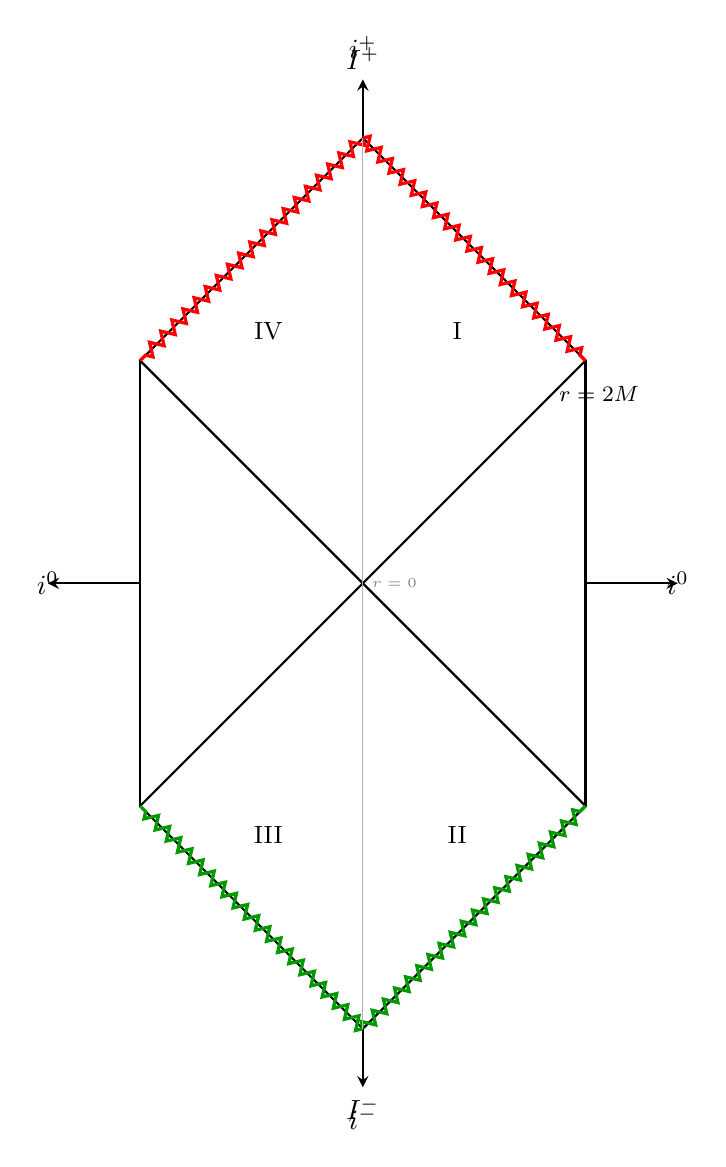
\begin{tikzpicture}[scale=4.0, >=stealth]
    % 钻石形边界
    \draw[thick] (0,0) -- (0.707,0.707) -- (0,1.414) -- (-0.707,0.707) -- cycle;
    \draw[thick] (0,0) -- (-0.707,-0.707) -- (0,-1.414) -- (0.707,-0.707) -- cycle;
    \draw[thick] (-0.707,0.707) -- (-0.707,-0.707);
    \draw[thick] (0.707,0.707) -- (0.707,-0.707);
    
    % 未来类光无穷远 I+
    \draw[thick, ->] (0,1.414) -- (0,1.6) node[above] {$\mathscr{I}^+$};
    % 过去类光无穷远 I-
    \draw[thick, ->] (0,-1.414) -- (0,-1.6) node[below] {$\mathscr{I}^-$};
    % 类空无穷远 i0
    \node at (1.0, 0) {$i^0$};
    \draw[thick, ->] (0.707,0) -- (1.0,0);
    \node at (-1.0, 0) {$i^0$};
    \draw[thick, ->] (-0.707,0) -- (-1.0,0);
    % 未来类时无穷远 i+
    \node at (0, 1.7) {$i^+$};
    % 过去类时无穷远 i-
    \node at (0, -1.7) {$i^-$};
    
    % 标签
    \node[font=\small] at (0.3, 0.8) {I};
    \node[font=\small] at (-0.3, 0.8) {IV};
    \node[font=\small] at (0.3, -0.8) {II};
    \node[font=\small] at (-0.3, -0.8) {III};
    
    % 奇点 (波浪线)
    \draw[red, very thick, decorate, decoration={zigzag, amplitude=0.8mm, segment length=2mm}] 
        (0,1.414) -- (0.707,0.707);
    \draw[red, very thick, decorate, decoration={zigzag, amplitude=0.8mm, segment length=2mm}] 
        (0,1.414) -- (-0.707,0.707);
    
    \draw[green!60!black, very thick, decorate, decoration={zigzag, amplitude=0.8mm, segment length=2mm}] 
        (0,-1.414) -- (0.707,-0.707);
    \draw[green!60!black, very thick, decorate, decoration={zigzag, amplitude=0.8mm, segment length=2mm}] 
        (0,-1.414) -- (-0.707,-0.707);
    
    % r=常数线
    \draw[gray!60, thin] (0,1.414) -- (0,-1.414);
    \node[font=\tiny, gray] at (0.1, 0.0) {$r=0$};
    
    % 视界标注
    \node[font=\footnotesize] at (0.75, 0.6) {$r=2M$};
\end{tikzpicture}
\caption{施瓦西时空的 Penrose 图（共形图）。整个无限时空被压缩到有限区域内，类光测地线以 $45^\circ$ 角传播。区域 I 是我们的宇宙，II 是黑洞，III 是白洞，IV 是另一个宇宙。$\mathscr{I}^\pm$ 是类光无穷远，$i^0$ 是类空无穷远，$i^\pm$ 是类时无穷远。波浪线表示曲率奇点 $r=0$。}
\label{fig:penrose}
\end{figure}

\begin{definition}[事件视界]
\textbf{事件视界 (event horizon)}是类光无穷远 $\mathscr{I}^+$ 的过去边界的边界——即所有不能到达 $\mathscr{I}^+$ 的事件构成的区域的边界。在施瓦西时空中，事件视界是 $r=2M$ 的类光超曲面：任何穿过 $r=2M$ 进入区域 II 的粒子或光线都无法再逃逸到区域 I。
\end{definition}

\section{Reissner–Nordström 与 Kerr 黑洞}
\label{sec:RN_Kerr}

\subsection{Reissner–Nordström 黑洞（带电黑洞）}

爱因斯坦–Maxwell 场方程描述了带电引力源的外度规。

\begin{definition}[Reissner–Nordström 度规]
质量为 $M$、电荷为 $Q$ 的球对称带电黑洞的度规为：
\begin{equation}
    \boxed{\dd s^2 = -\Delta(r)\,\dd t^2 + \Delta(r)^{-1}\,\dd r^2 + r^2\,\dd\Omega^2},
    \label{eq:RN_metric}
\end{equation}
其中 $\Delta(r) \equiv 1 - \frac{2M}{r} + \frac{Q^2}{r^2}$。相应的电磁场为 $F = \frac{Q}{r^2}\,\dd t \wedge \dd r$。
\end{definition}

\begin{theorem}[RN 黑洞的视界结构]
$\Delta(r)=0$ 的根给出视界位置：
\begin{equation}
    r_\pm = M \pm \sqrt{M^2 - Q^2}.
\end{equation}
根据 $Q$ 与 $M$ 的关系，分三种情况：
\begin{itemize}
    \item $|Q| < M$：\textbf{次极端 RN 黑洞}——有两个视界：$r_+$（外视界/事件视界），$r_-$（内视界/Cauchy 视界）；
    \item $|Q| = M$：\textbf{极端 RN 黑洞}——$r_+ = r_- = M$，单一退化视界，表面引力 $\kappa = 0$；
    \item $|Q| > M$：\textbf{裸奇点}——没有视界，奇点 $r=0$ 是裸露的。宇宙监督假设 (Cosmic Censorship) 推测这种情况在物理上不会发生 \cite{Penrose1965}。
\end{itemize}
\end{theorem}

\subsection{Kerr 黑洞（旋转黑洞）}

Roy Kerr 于 1963 年发现了描述旋转黑洞的精确解——这是天体物理中最重要的一类黑洞，因为实际黑洞通常具有角动量。

\begin{definition}[Kerr 度规 —— Boyer–Lindquist 坐标]
在 Boyer–Lindquist 坐标 $(t,r,\theta,\phi)$ 中，质量为 $M$、角动量为 $J = aM$ 的 Kerr 度规为：
\begin{equation}
    \boxed{\dd s^2 = -\left(1-\frac{2Mr}{\Sigma}\right)\dd t^2 - \frac{4aMr\sin^2\theta}{\Sigma}\,\dd t\dd\phi + \frac{\Sigma}{\Delta}\,\dd r^2 + \Sigma\,\dd\theta^2 + \left(r^2+a^2+\frac{2Mra^2\sin^2\theta}{\Sigma}\right)\sin^2\theta\,\dd\phi^2},
    \label{eq:Kerr_metric}
\end{equation}
其中：
\begin{equation}
    \Sigma \equiv r^2 + a^2\cos^2\theta, \qquad \Delta \equiv r^2 - 2Mr + a^2.
\end{equation}
参数 $a \equiv J/M$ 是\textbf{比角动量 (specific angular momentum)}，满足 $0 \leq a \leq M$。
\end{definition}

\begin{theorem}[Kerr 黑洞的视界与能层]
$\Delta = 0$ 给出两个视界：
\begin{equation}
    r_\pm = M \pm \sqrt{M^2 - a^2}.
\end{equation}
$g_{tt}=0$ 给出\textbf{静界 (static limit)}：
\begin{equation}
    r_{\text{sl}}(\theta) = M + \sqrt{M^2 - a^2\cos^2\theta}.
\end{equation}
视界 $r_+$ 与静界之间的区域称为\textbf{能层 (ergosphere)}。在能层内，任何观者必须随黑洞旋转——无法保持静态（相对于无穷远观者静止），但仍可以逃逸到无穷远。
\end{theorem}

\begin{note}[Penrose 过程 —— 从旋转黑洞提取能量]
在能层中，粒子可以分裂为两部分：一部分落入黑洞（负能量轨道），另一部分逃逸到无穷远——带着比原粒子更多的能量。这个过程称为\textbf{Penrose 过程}，理论上可以从旋转黑洞中提取旋转能。可提取的最大能量为 $M - M_{\text{irr}}$，其中不可约质量 $M_{\text{irr}} = \sqrt{\frac{1}{2}(M^2 + \sqrt{M^4 - J^2})}$。极端 Kerr 黑洞（$a=M$）中多达 $29\%$ 的质量能量可以被提取 \cite{Misner1973}。
\end{note}

\subsection{Kerr–Newman 黑洞}

最一般的稳态黑洞解是 Kerr–Newman 度规，包含质量 $M$、电荷 $Q$ 和角动量 $a$：
\begin{equation}
    \Delta = r^2 - 2Mr + a^2 + Q^2, \qquad \Sigma = r^2 + a^2\cos^2\theta.
\end{equation}
视界位于 $\Delta=0$ 的根：$r_\pm = M \pm \sqrt{M^2 - a^2 - Q^2}$。极端条件为 $M^2 = a^2 + Q^2$。

\subsection{无毛定理 (No-hair Theorem)}

\begin{theorem}[黑洞无毛定理]
在四维爱因斯坦–Maxwell 理论中，稳态黑洞由且仅由三个参数完全描述：
\begin{equation}
    \boxed{M\;(\text{质量}),\quad J\;(\text{角动量}),\quad Q\;(\text{电荷})}.
\end{equation}
所有其他信息（如形成黑洞的物质的初始多极矩）在引力坍缩过程中被辐射掉了。黑洞是“最简单”的宏观物体 \cite{Wald1984,Carroll1997}。
\end{theorem}

\section{黑洞热力学}
\label{sec:BH_thermo}

黑洞热力学是 20 世纪理论物理学最深刻的发现之一——它揭示了引力、量子力学和热力学之间的深层联系。

\subsection{黑洞力学四定律}

\begin{theorem}[黑洞力学四定律]
\label{thm:four_laws}
\begin{enumerate}
    \item \textbf{第零定律}：稳态黑洞的\textbf{表面引力 (surface gravity)} $\kappa$ 在视界上处处为常数（类似于热力学第零定律中温度的均匀性）。
    
    \item \textbf{第一定律}：黑洞质量 $M$、面积 $A$、角动量 $J$ 和电荷 $Q$ 满足：
    \begin{equation}
        \boxed{\dd M = \frac{\kappa}{8\pi G}\,\dd A + \Omega_H\,\dd J + \Phi_H\,\dd Q},
        \label{eq:first_law}
    \end{equation}
    其中 $\Omega_H$ 是视界角速度，$\Phi_H$ 是视界电势。这类似于热力学第一定律 $\dd U = T\dd S + \Omega\dd J + \Phi\dd Q$。
    
    \item \textbf{第二定律 (Hawking 面积定理)}：在经典广义相对论中（满足零能量条件），黑洞视界面积永不减少：
    \begin{equation}
        \boxed{\delta A \geq 0}.
        \label{eq:area_theorem}
    \end{equation}
    这类似于热力学第二定律中熵的单调增加。
    
    \item \textbf{第三定律}：不能通过任何有限步骤将黑洞的表面引力 $\kappa$ 降为零（即不能形成极端黑洞）。这类似于热力学第三定律中不能通过有限步骤达到绝对零度。
\end{enumerate}
\end{theorem}

\subsection{Bekenstein–Hawking 熵}

最初，黑洞力学四定律被认为仅是形式上的类比——毕竟，经典黑洞只能吸收、不能辐射，按定义温度应为零。1972 年，Jacob Bekenstein 大胆提出：黑洞面积\textbf{就是}熵（乘以适当常数），黑洞具有真实的\textbf{热力学}性质 \cite{Wald1984}。

\begin{theorem}[Bekenstein–Hawking 熵公式]
黑洞的熵正比于其视界面积：
\begin{equation}
    \boxed{S_{\text{BH}} = \frac{k_B c^3 A}{4G\hbar} = \frac{A}{4G} \quad (\text{Planck 单位: } k_B = \hbar = c = 1)}.
    \label{eq:BH_entropy}
\end{equation}
在 Planck 单位制中（$G = \ell_P^2$），$S = A/(4\ell_P^2)$——即视界的每个 Planck 面积单元承载约 $\frac{1}{4}\ln 2$ 比特的信息。
\end{theorem}

\begin{note}[广义第二定律]
Bekenstein 提出了\textbf{广义第二定律 (Generalized Second Law, GSL)}：黑洞外物质熵 $S_{\text{matter}}$ 与黑洞熵 $S_{\text{BH}}$ 之和永不减少：
\begin{equation}
    \delta(S_{\text{BH}} + S_{\text{matter}}) \geq 0.
\end{equation}
GSL 将热力学第二定律推广到了包含黑洞的系统中。
\end{note}

\subsection{Hawking 辐射}

1974 年，Stephen Hawking 做出了划时代的发现：将量子场论应用于黑洞时空背景，黑洞\textbf{确实会辐射}——而且是以精确的热谱辐射！

\begin{theorem}[Hawking 辐射与黑洞温度]
施瓦西黑洞以温度为 $T_H$ 的黑体谱辐射粒子：
\begin{equation}
    \boxed{T_H = \frac{\hbar c^3}{8\pi G M k_B} = \frac{\hbar \kappa}{2\pi k_B c} \quad (\text{其中 } \kappa = \frac{c^4}{4GM} \text{ 是表面引力})}.
    \label{eq:Hawking_temp}
\end{equation}
在 Planck 单位中：$T_H = 1/(8\pi M)$。对于太阳质量的黑洞，$T_H \sim 6\times10^{-8}\,\text{K}$——远低于宇宙微波背景温度，因此天体物理黑洞是净吸收者。对于微型原初黑洞（$M \sim 10^{15}\,\text{g}$），$T_H \sim 10^{11}\,\text{K}$，会剧烈蒸发 \cite{Hawking1974}。
\end{theorem}

\begin{note}[Hawking 辐射的物理图像]
量子场论在弯曲时空中的真空不稳定性导致粒子对的产生：在视界附近，虚粒子对中的一个可能落入黑洞（携带负能量），另一个逃逸到无穷远（表现为正能量粒子）。净效果是黑洞质量减少——黑洞“蒸发”。这统一了黑洞力学四定律与真实的热力学：$\kappa/(2\pi)$ 就是黑洞的物理温度，$A/(4G)$ 就是黑洞的物理熵。
\end{note}

\subsection{黑洞热力学与全息原理}

Bekenstein–Hawking 熵公式 $S = A/(4G)$ 具有深远的意义：熵（通常被认为是广延量，正比于体积）在这里正比于\textbf{面积}。这暗示了\textbf{全息原理 (Holographic Principle)}——量子引力理论中，一个空间区域内的全部信息可以编码在该区域的边界上。这是 AdS/CFT 对偶和量子引力研究中的核心思想。

\section{算例与验证}
\label{sec:examples}

\subsection{例 1：计算 ISCO 处的轨道角速度}

对于施瓦西黑洞 $r_{\text{ISCO}} = 6M$ 处的圆轨道：
\begin{equation}
    \Omega = \frac{\dd\phi}{\dd t} = \frac{\dot\phi}{\dot t} = \frac{L/r^2}{E/(1-2M/r)}.
\end{equation}
在 $r=6M$ 处，$L=2\sqrt{3}M$，$E=2\sqrt{2}/3$，代入得：
\begin{equation}
    \Omega_{\text{ISCO}} = \frac{1}{6\sqrt{6}M} \approx \frac{0.068}{M}.
\end{equation}
对应的轨道周期为 $T = 2\pi/\Omega \approx 92.3M$。

\subsection{例 2：Eddington–Finkelstein 坐标中验证 $r=2M$ 处度规正则}

在 Eddington–Finkelstein 坐标（\ref{eq:EF_metric}）中，度规分量为：
\begin{equation}
    g_{vv} = -\left(1-\frac{2M}{r}\right), \quad g_{vr}=g_{rv}=1, \quad g_{rr}=0, \quad g_{\theta\theta}=r^2, \quad g_{\phi\phi}=r^2\sin^2\theta.
\end{equation}
在 $r=2M$ 处，$g_{vv}=0$，$g_{vr}=1$，$g_{rr}=0$。行列式：
\begin{equation}
    \det(g_{\mu\nu}) = -r^4\sin^2\theta \neq 0 \quad (\text{在 } r=2M \text{ 处仍非零}).
\end{equation}
所有度规分量都是有限且可逆的——度规在 $r=2M$ 处完全正则。

\subsection{例 3：验证 $r=2M$ 是类光超曲面}

$r=2M$ 超曲面的法矢量为 $n_\mu = \partial_\mu r = (0,1,0,0)$。其模方为：
\begin{equation}
    g^{\mu\nu}n_\mu n_\nu = g^{rr} = 1 - \frac{2M}{r}.
\end{equation}
在 $r=2M$ 处，$g^{rr}=0$——法矢量是\textbf{类光}的（模方为零）。因此 $r=2M$ 是一个\textbf{类光超曲面 (null hypersurface)}，这正是事件视界的定义特征：它是单向膜——粒子只能向 $r$ 减小的方向穿过它。验证：在 Eddington–Finkelstein 坐标中，入射类光测地线 $v=\text{常数}$ 穿过 $r=2M$ 时满足 $\dd r/\dd\lambda < 0$ 对于正向仿射参数永远成立。

\subsection{例 4：计算太阳质量黑洞的 Hawking 温度与蒸发时间}

取 $M = M_\odot \approx 2\times10^{30}\,\text{kg}$。
\begin{align}
    T_H &= \frac{\hbar c^3}{8\pi G M k_B} \approx 6.2\times10^{-8}\,\text{K}, \\
    r_s &= \frac{2GM}{c^2} \approx 3.0\,\text{km}, \\
    A &= 4\pi r_s^2 \approx 1.1\times10^{8}\,\text{m}^2, \\
    S_{\text{BH}} &= \frac{k_B A}{4\ell_P^2} \approx 1.1\times10^{77}\,k_B.
\end{align}
由 Stefan–Boltzmann 定律（近似），蒸发时间尺度为：
\begin{equation}
    \tau_{\text{evap}} \sim \frac{M^3}{3\alpha}, \qquad \alpha \sim 10^{-4} \;\Longrightarrow\; \tau_{\text{evap}} \sim 10^{67}\,\text{年},
\end{equation}
远大于宇宙年龄（$\sim 1.38\times10^{10}$ 年）——天体物理黑洞在当前宇宙中几乎不蒸发。

\subsection{例 5：Kruskal 坐标中的类时 Killing 矢量}

在 Kruskal 坐标中，$\xi_{(t)} = \partial_t$ 变为：
\begin{equation}
    \xi_{(t)} = \frac{1}{4M}\left(X\,\partial_T + T\,\partial_X\right).
\end{equation}
其模方为：
\begin{equation}
    \xi_{(t)}^\mu \xi_{(t)\mu} = -\left(1-\frac{2M}{r}\right) = \frac{2M}{r}\cdot\frac{T^2-X^2}{T^2-X^2} \cdot (\text{因子}).
\end{equation}
在 $r=2M$（$T^2=X^2$）处，$\xi_{(t)}$ 是类光的；在 $r<2M$（$T^2>X^2$）处，$\xi_{(t)}$ 变为类空——在黑洞内部，$t$ 不再是时间坐标，$r$ 才是时间坐标。这完美展示了事件视界作为“时间与空间角色互换”的边界 \cite{Carroll1997}。

\section*{本章小结}

施瓦西解是爱因斯坦场方程最简单却最重要的精确解。Birkhoff 定理确保球对称真空解必然是静态的施瓦西度规。通过分析 Killing 矢量与守恒量 $E$ 和 $L$，测地线问题简化为有效势的一维运动。广义相对论修正项 $-ML^2/r^3$ 导致 ISCO 在 $r=6M$、光子球在 $r=3M$，以及近日点进动 $\Delta\phi = 6\pi M/[a(1-e^2)]$。

坐标奇点 $r=2M$ 可通过 Eddington–Finkelstein 或 Kruskal–Szekeres 坐标消除，揭示 $r=2M$ 是事件视界——一个类光超曲面。Kruskal 最大解析延拓展现了四个区域：两个渐近平坦宇宙、一个黑洞和一个白洞。推广到带电（RN）和旋转（Kerr）黑洞引入了更丰富的视界结构、能层和 Penrose 过程。

黑洞热力学将经典黑洞力学四定律与真实的热力学统一起来。Bekenstein 熵 $S = A/(4G)$ 和 Hawking 温度 $T_H = \kappa/(2\pi)$ 揭示了引力、量子和热力学的深层联系，为全息原理和量子引力研究铺平了道路。黑洞不再仅是“引力监狱”——它们是具有温度、熵的热力学系统，能够通过 Hawking 辐射缓慢蒸发。黑洞物理是 21 世纪理论物理最活跃的前沿领域之一。
  % 施瓦西解与黑洞
% chapter12.tex - 引力波
\chapter{引力波 (Gravitational Waves)}
\label{chap:GW}

\section{引力波的物理图像}
\label{sec:GW_physical_picture}

爱因斯坦在1916年就预言了引力波的存在——时空度规的微小涟漪以光速传播。这是广义相对论最引人注目的预言之一，但直到整整一个世纪之后的2015年，才被激光干涉引力波天文台（LIGO）首次直接探测到 \cite{Abbott2016}。本章的推导和讨论参考了经典文献 \cite{Carroll1997,Misner1973,Wald1984}。

引力波的本质可以从电磁波的类比来理解。在电动力学中，加速运动的电荷辐射电磁波——电场和磁场的振荡以光速传播。在广义相对论中，时空本身就是动力学实体，加速运动的质量（或更准确地说，质量四极矩随时间变化）辐射引力波——时空曲率的振荡以光速传播。

\begin{note}[引力波与电磁波的对比]
\begin{center}
\begin{tabular}{l|l}
\hline
\textbf{电磁波} & \textbf{引力波} \\ \hline
源：加速电荷 & 源：加速质量（四极矩变化） \\
最低阶辐射：偶极辐射 & 最低阶辐射：四极辐射 \\
偏振：两个矢量偏振态 & 偏振：两个张量偏振态（$+$ 和 $\times$） \\
介质：电磁场 & 介质：时空本身 \\
速度：$c$（在介质中可改变） & $c$（在所有介质中不变） \\
\hline
\end{tabular}
\end{center}
\end{note}

为什么引力波的最低阶辐射是四极辐射而非偶极辐射？原因有二：（1）质量守恒禁止了质量偶极辐射（不存在负质量，无法构成振荡偶极）；（2）动量守恒禁止了质量流偶极辐射（孤立系统的质心匀速运动）。因此引力波辐射的第一个非平凡阶是四极辐射——由质量四极矩的二阶时间导数驱动。

\begin{property}[引力波的基本特征]
\begin{enumerate}
    \item \textbf{横波性}：引力波是横波，振动方向垂直于传播方向
    \item \textbf{两个偏振态}：$+$ 模（plus mode）和 $\times$ 模（cross mode），相差 $45^\circ$
    \item \textbf{以光速传播}：$v = c$，与频率无关（无介质色散）
    \item \textbf{潮汐效应}：引力波拉伸一个横向尺度同时压缩另一个正交横向尺度
    \item \textbf{极其微弱}：到达地球的引力波典型应变为 $h \sim 10^{-21}$，相当于测量地球-太阳距离（$1.5\times10^{11}$ m）时精确到一个原子直径（$10^{-10}$ m）的量级
\end{enumerate}
\end{property}

\section{线性化引力}
\label{sec:linearized_gravity}

\subsection{弱场展开}

当引力场足够弱时，时空度规可以写为平坦 Minkowski 背景加上微小扰动：

\begin{definition}[弱场度规]
\begin{equation}
    \boxed{g_{\mu\nu} = \eta_{\mu\nu} + h_{\mu\nu}}, \qquad |h_{\mu\nu}| \ll 1.
    \label{eq:weak_field}
\end{equation}
其中 $\eta_{\mu\nu} = \diag(-1, +1, +1, +1)$ 是 Minkowski 度规，$h_{\mu\nu}$ 是度规扰动张量。以下所有计算只保留 $h_{\mu\nu}$ 的\textbf{一阶项}，忽略 $\Order(h^2)$ 及更高阶，这就是\textbf{线性化引力}。
\end{definition}

在一阶近似下，指标升降使用背景度规 $\eta^{\mu\nu}$：
\begin{equation}
    g^{\mu\nu} = \eta^{\mu\nu} - h^{\mu\nu} + \Order(h^2), \qquad h^{\mu\nu} \equiv \eta^{\mu\rho}\eta^{\nu\sigma}h_{\rho\sigma}.
\end{equation}
注意 $h^\mu{}_\nu = \eta^{\mu\rho}h_{\rho\nu}$ 和 $h = \eta^{\mu\nu}h_{\mu\nu} = h^\mu{}_\mu$。

\subsection{线性化的联络与曲率}

到 $h$ 的一阶，Christoffel 符号为：
\begin{equation}
    \Gamma^\mu_{\nu\rho} = \frac{1}{2}\eta^{\mu\sigma}\left(\partial_\nu h_{\rho\sigma} + \partial_\rho h_{\nu\sigma} - \partial_\sigma h_{\nu\rho}\right) + \Order(h^2).
    \label{eq:linear_Gamma}
\end{equation}

线性化的 Riemann 张量（到一阶）：
\begin{equation}
    R^\mu{}_{\nu\rho\sigma} = \partial_\rho\Gamma^\mu_{\sigma\nu} - \partial_\sigma\Gamma^\mu_{\rho\nu} + \Order(h^2).
\end{equation}
代入式 (\ref{eq:linear_Gamma})，得到：
\begin{equation}
    R_{\mu\nu\rho\sigma} = \frac{1}{2}\left(\partial_\nu\partial_\rho h_{\mu\sigma} + \partial_\mu\partial_\sigma h_{\nu\rho} - \partial_\mu\partial_\rho h_{\nu\sigma} - \partial_\nu\partial_\sigma h_{\mu\rho}\right).
    \label{eq:linear_Riemann}
\end{equation}

线性化的 Ricci 张量和标量曲率：
\begin{align}
    R_{\mu\nu} &= \eta^{\rho\sigma}R_{\rho\mu\sigma\nu} \nonumber\\
    &= \frac{1}{2}\left(\partial^\rho\partial_\mu h_{\nu\rho} + \partial^\rho\partial_\nu h_{\mu\rho} - \Box h_{\mu\nu} - \partial_\mu\partial_\nu h\right),
    \label{eq:linear_Ricci}
\end{align}
其中 $\Box \equiv \eta^{\mu\nu}\partial_\mu\partial_\nu = -\partial_t^2 + \nabla^2$ 是平坦时空中的达朗贝尔算子（这里取 $c=1$），$h = \eta^{\mu\nu}h_{\mu\nu}$ 是扰动的迹。

\begin{align}
    R &= \eta^{\mu\nu}R_{\mu\nu} = \partial^\mu\partial^\nu h_{\mu\nu} - \Box h.
    \label{eq:linear_Rscalar}
\end{align}

Einstein 张量的线性化形式为：
\begin{equation}
    G_{\mu\nu} = R_{\mu\nu} - \frac{1}{2}R\,\eta_{\mu\nu}
    = \frac{1}{2}\left(\partial^\rho\partial_\mu h_{\nu\rho} + \partial^\rho\partial_\nu h_{\mu\rho} - \Box h_{\mu\nu} - \partial_\mu\partial_\nu h - \eta_{\mu\nu}\partial^\rho\partial^\sigma h_{\rho\sigma} + \eta_{\mu\nu}\Box h\right).
    \label{eq:linear_Einstein}
\end{equation}

\subsection{规范自由与坐标变换}

线性化引力具有\textbf{规范对称性}——它是广义相对论微分同胚不变性在线性化近似中的残留。考虑无穷小坐标变换：
\begin{equation}
    x^\mu \to x'^\mu = x^\mu + \xi^\mu(x),
\end{equation}
其中 $|\partial_\mu\xi^\nu| \sim \Order(h)$ 与 $h_{\mu\nu}$ 同阶。度规的张量变换律 $g'_{\mu\nu}(x') = \frac{\partial x^\rho}{\partial x'^\mu}\frac{\partial x^\sigma}{\partial x'^\nu} g_{\rho\sigma}(x)$ 在线性阶给出：
\begin{equation}
    \boxed{h_{\mu\nu} \to h'_{\mu\nu} = h_{\mu\nu} - \partial_\mu\xi_\nu - \partial_\nu\xi_\mu}.
    \label{eq:gauge_trans}
\end{equation}
这里 $\xi_\mu = \eta_{\mu\nu}\xi^\nu$。这一变换称为\textbf{规范变换}，与电磁学中的 $A_\mu \to A_\mu + \partial_\mu\Lambda$ 完全类似。

\begin{note}[规范不变性]
可以验证，线性化的 Riemann 张量 (\ref{eq:linear_Riemann})、Ricci 张量 (\ref{eq:linear_Ricci}) 和 Einstein 张量 (\ref{eq:linear_Einstein}) 在规范变换 (\ref{eq:gauge_trans}) 下都是不变的。这意味着物理可观测量（如测地线偏离）不依赖于规范选择——规范只是描述上的冗余。
\end{note}

\section{引力波方程}
\label{sec:GW_equation}

\subsection{迹反转变量与 Lorenz 规范}

为了简化线性化的 Einstein 方程，引入\textbf{迹反转扰动 (trace-reversed perturbation)}：

\begin{definition}[迹反转变量]
\begin{equation}
    \boxed{\bar{h}_{\mu\nu} \equiv h_{\mu\nu} - \frac{1}{2}\eta_{\mu\nu}h}.
    \label{eq:bar_h}
\end{equation}
其逆关系为 $h_{\mu\nu} = \bar{h}_{\mu\nu} - \frac{1}{2}\eta_{\mu\nu}\bar{h}$，其中 $\bar{h} = \eta^{\mu\nu}\bar{h}_{\mu\nu} = -h$。
\end{definition}

将 $\bar{h}_{\mu\nu}$ 代入 Einstein 张量 (\ref{eq:linear_Einstein})，经过冗长但直接的代数化简（使用 $\partial_\mu\eta^{\mu\nu}=0$ 和交换偏导数），得到：
\begin{equation}
    G_{\mu\nu} = -\frac{1}{2}\left[\Box \bar{h}_{\mu\nu} + \eta_{\mu\nu}\partial^\rho\partial^\sigma\bar{h}_{\rho\sigma} - \partial^\rho\partial_\nu\bar{h}_{\mu\rho} - \partial^\rho\partial_\mu\bar{h}_{\nu\rho}\right].
    \label{eq:Einstein_barh}
\end{equation}

现在选择规范来消去多余的项。类似电动力学中的 Lorentz 规范 $\partial^\mu A_\mu = 0$，在引力中我们选择：

\begin{definition}[Lorenz 规范 / 谐和规范]
\begin{equation}
    \boxed{\partial^\mu \bar{h}_{\mu\nu} = 0}.
    \label{eq:Lorenz_gauge}
\end{equation}
这一规范条件也称为\textbf{谐和坐标条件 (harmonic coordinate condition)}，因为 $\Box x^\mu = 0$。
\end{definition}

在 Lorenz 规范下，式 (\ref{eq:Einstein_barh}) 中后三项全部消失，Einstein 方程简化为平坦时空中的波动方程：

\begin{theorem}[线性化 Einstein 方程 —— 引力波方程]
在 Lorenz 规范 $\partial^\mu\bar{h}_{\mu\nu}=0$ 下，线性化的 Einstein 场方程变为：
\begin{equation}
    \boxed{\Box \bar{h}_{\mu\nu} = -\frac{16\pi G}{c^4} T_{\mu\nu}}.
    \label{eq:wave_equation}
\end{equation}
这里恢复了 $c$。在真空中（$T_{\mu\nu}=0$），方程为 $\Box\bar{h}_{\mu\nu} = 0$ —— 正是以光速 $c$ 传播的波动方程。
\end{theorem}

\begin{proof}
线性化的 Einstein 方程 $G_{\mu\nu} = \frac{8\pi G}{c^4}T_{\mu\nu}$（恢复 $c$）。利用式 (\ref{eq:Einstein_barh})，在 Lorenz 规范下，包含 $\partial^\mu\bar{h}_{\mu\nu}$ 的项全部为零，$G_{\mu\nu} = -\frac{1}{2}\Box\bar{h}_{\mu\nu}$。因此：
\begin{equation}
    -\frac{1}{2}\Box\bar{h}_{\mu\nu} = \frac{8\pi G}{c^4}T_{\mu\nu}
    \quad\Longrightarrow\quad
    \Box\bar{h}_{\mu\nu} = -\frac{16\pi G}{c^4}T_{\mu\nu}.
\end{equation}
\end{proof}

\subsection{TT 规范（横无迹规范）}

Lorenz 规范并未完全固定所有规范自由度。在真空中（$T_{\mu\nu}=0$），$\Box\bar{h}_{\mu\nu}=0$，但 $\bar{h}_{\mu\nu}$ 仍有 10 个独立分量，受 4 个 Lorenz 条件 $\partial^\mu\bar{h}_{\mu\nu}=0$ 约束。剩余的 6 个分量中，还有 4 个可以通过进一步的规范变换消去（在真空中可以保持 Lorenz 规范的同时进行此类变换）。最终只剩下 2 个物理自由度。

\begin{definition}[TT 规范 —— 横无迹规范]
对于沿 $z$ 方向传播的平面引力波，\textbf{TT 规范 (Transverse-Traceless gauge)} 由以下条件定义：
\begin{equation}
    \bar{h}_{0\mu} = 0, \qquad \bar{h}^\mu{}_\mu = 0, \qquad \partial^j \bar{h}_{ij} = 0.
    \label{eq:TT_gauge}
\end{equation}
在 TT 规范中，$\bar{h}_{\mu\nu} = h_{\mu\nu}^{\text{TT}}$（因为无迹意味着 $h=0$，从而 $\bar{h}_{\mu\nu}=h_{\mu\nu}$）。
\end{definition}

对于沿 $+z$ 方向传播的平面引力波，TT 规范中的度规扰动具有如下形式：
\begin{equation}
    h_{\mu\nu}^{\text{TT}} = 
    \begin{pmatrix}
        0 & 0 & 0 & 0 \\
        0 & h_+ & h_\times & 0 \\
        0 & h_\times & -h_+ & 0 \\
        0 & 0 & 0 & 0
    \end{pmatrix},
    \label{eq:TT_matrix}
\end{equation}
其中 $h_+ = h_+(t-z/c)$ 和 $h_\times = h_\times(t-z/c)$ 是沿 $z$ 方向传播的两个独立偏振模式。这是一个横波：只有空间分量且垂直于传播方向（$x$-$y$ 平面），无迹（$h_{11}+h_{22}=0$）。

\section{引力波的偏振}
\label{sec:polarization}

\subsection{两个偏振态的物理效应}

考虑一排自由测试粒子排列在垂直于引力波传播方向的圆环上。当引力波通过时，TT 规范意味着测试粒子的坐标保持不变（$\dd^2 x^i/\dd\tau^2 = 0$），但\textbf{固有距离}随时间振荡。$h_+$ 偏振和 $h_\times$ 偏振对圆环测试粒子的效应如下：

\begin{figure}[htbp]
\centering
\begin{tikzpicture}[scale=2.8, >=stealth]

    % --- h_+ 偏振 ---
    \node[font=\bfseries] at (0, 1.4) {$h_+$ 偏振};
    
    % 未形变圆 (虚线)
    \draw[dashed, gray, thick] (0,0) circle (1.0);
    
    % 时刻 0: 未形变
    \draw[gray, thick] (0,0) circle (1.0);
    \foreach \ang in {0, 45, 90, 135, 180, 225, 270, 315} {
        \fill[gray] (\ang:{1.0}) circle (0.04);
    }
    \node at (0, -1.3) {$t = 0$};
    
    % 时刻 T/4: 水平拉伸, 竖直压缩
    \begin{scope}[xshift=3.5cm]
        \draw[blue, thick] (0,0) ellipse (1.2 and 0.8);
        \foreach \ang in {0, 45, 90, 135, 180, 225, 270, 315} {
            \pgfmathsetmacro{\rx}{1.2}
            \pgfmathsetmacro{\ry}{0.8}
            \pgfmathsetmacro{\px}{\rx*cos(\ang)}
            \pgfmathsetmacro{\py}{\ry*sin(\ang)}
            \fill[blue] (\px, \py) circle (0.04);
        }
        \node at (0, -1.3) {$t = T/4$};
    \end{scope}

    % 时刻 T/2: 未形变
    \begin{scope}[xshift=7.0cm]
        \draw[gray, thick] (0,0) circle (1.0);
        \foreach \ang in {0, 45, 90, 135, 180, 225, 270, 315} {
            \fill[gray] (\ang:{1.0}) circle (0.04);
        }
        \node at (0, -1.3) {$t = T/2$};
    \end{scope}

    % 时刻 3T/4: 竖直拉伸, 水平压缩
    \begin{scope}[xshift=10.5cm]
        \draw[red, thick] (0,0) ellipse (0.8 and 1.2);
        \foreach \ang in {0, 45, 90, 135, 180, 225, 270, 315} {
            \pgfmathsetmacro{\rx}{0.8}
            \pgfmathsetmacro{\ry}{1.2}
            \pgfmathsetmacro{\px}{\rx*cos(\ang)}
            \pgfmathsetmacro{\py}{\ry*sin(\ang)}
            \fill[red] (\px, \py) circle (0.04);
        }
        \node at (0, -1.3) {$t = 3T/4$};
    \end{scope}

    % --- h_× 偏振 (下一行) ---
    \node[font=\bfseries] at (0, -2.5) {$h_\times$ 偏振};
    
    % 未形变
    \begin{scope}[yshift=-3.5cm]
        \draw[gray, thick] (0,0) circle (1.0);
        \foreach \ang in {0, 45, 90, 135, 180, 225, 270, 315} {
            \fill[gray] (\ang:{1.0}) circle (0.04);
        }
        \foreach \ang in {45, 135, 225, 315} {
            \draw[gray, thin, densely dotted] (0,0) -- (\ang:1.3);
        }
        \node at (0, -1.3) {$t = 0$};
    \end{scope}

    % T/4: 对角线拉伸
    \begin{scope}[xshift=3.5cm, yshift=-3.5cm]
        % 旋转45度的椭圆
        \begin{scope}[rotate=45]
            \draw[blue, thick] (0,0) ellipse (1.2 and 0.8);
        \end{scope}
        \foreach \ang in {0, 45, 90, 135, 180, 225, 270, 315} {
            \pgfmathsetmacro{\rx}{1.2}
            \pgfmathsetmacro{\ry}{0.8}
            \pgfmathsetmacro{\px}{\rx*cos(\ang-45)*cos(45) - \ry*sin(\ang-45)*sin(45)}
            \pgfmathsetmacro{\py}{\rx*cos(\ang-45)*sin(45) + \ry*sin(\ang-45)*cos(45)}
            \fill[blue] (\px, \py) circle (0.04);
        }
        \node at (0, -1.3) {$t = T/4$};
    \end{scope}

    % T/2: 未形变
    \begin{scope}[xshift=7.0cm, yshift=-3.5cm]
        \draw[gray, thick] (0,0) circle (1.0);
        \foreach \ang in {0, 45, 90, 135, 180, 225, 270, 315} {
            \fill[gray] (\ang:{1.0}) circle (0.04);
        }
        \node at (0, -1.3) {$t = T/2$};
    \end{scope}

    % 3T/4: 反对角线拉伸
    \begin{scope}[xshift=10.5cm, yshift=-3.5cm]
        \begin{scope}[rotate=45]
            \draw[red, thick] (0,0) ellipse (0.8 and 1.2);
        \end{scope}
        \foreach \ang in {0, 45, 90, 135, 180, 225, 270, 315} {
            \pgfmathsetmacro{\rx}{0.8}
            \pgfmathsetmacro{\ry}{1.2}
            \pgfmathsetmacro{\px}{\rx*cos(\ang-45)*cos(45) - \ry*sin(\ang-45)*sin(45)}
            \pgfmathsetmacro{\py}{\rx*cos(\ang-45)*sin(45) + \ry*sin(\ang-45)*cos(45)}
            \fill[red] (\px, \py) circle (0.04);
        }
        \node at (0, -1.3) {$t = 3T/4$};
    \end{scope}

\end{tikzpicture}
\caption{引力波两种偏振态对环形测试粒子的效应。$h_+$ 模交替沿 $x$ 轴和 $y$ 轴方向拉伸/压缩环；$h_\times$ 模则沿 $45^\circ$ 对角线方向拉伸/压缩。两种模式周期相同但相差 $45^\circ$ 空间旋转。注意 TT 规范中测试粒子的坐标不变，改变的是它们之间的固有距离。}
\label{fig:polarization}
\end{figure}

\begin{note}[测地线偏离与引力波探测]
图 \ref{fig:polarization} 揭示了引力波探测的基本原理。当引力波通过时，自由粒子之间的\textbf{固有距离}发生振荡。这正是 LIGO 等干涉仪探测引力波的核心思想：激光干涉仪测量两个垂直臂中悬挂的镜面之间的距离变化——即引力波导致的潮汐形变。$h_+$ 模使一臂拉伸而另一臂压缩，$h_\times$ 模亦然但旋转 $45^\circ$。
\end{note}

\subsection{物质对引力波的响应}

在 TT 规范中，线性化的测地线偏离方程为：
\begin{equation}
    \frac{\dd^2 \xi^i}{\dd t^2} = -R^i{}_{0j0}\,\xi^j = \frac{1}{2}\ddot{h}_{ij}^{\text{TT}}\,\xi^j,
    \label{eq:geodesic_deviation}
\end{equation}
其中 $\xi^i$ 是两相邻自由粒子之间的偏离矢量。对于 $h_+$ 偏振，初始在 $(x_0, y_0)$ 的粒子感受到的加速度为：
\begin{equation}
    \ddot{x} = \frac{1}{2}\ddot{h}_+ x_0, \qquad \ddot{y} = -\frac{1}{2}\ddot{h}_+ y_0.
\end{equation}
这正是图 \ref{fig:polarization} 中描绘的拉伸-压缩模式。

\section{引力波的能量辐射}
\label{sec:energy_radiation}

\subsection{Isaacson 有效能量-动量张量}

引力波携带能量——这是引力场非线性的直接体现。然而，在广义相对论中定义引力场的局部能量是一个微妙的问题（由等效原理导致）。解决之道由 Isaacson 提出：通过将度规分离为慢变背景和快变引力波，在几个波长的尺度上作\textbf{Brill--Hartle 平均}，可以构造一个规范不变的\textbf{有效能量-动量张量}。

\begin{definition}[Isaacson 能量-动量张量]
引力波的有效能量-动量张量由度规扰动的二阶项通过 Brill--Hartle 平均给出：
\begin{equation}
    \boxed{T_{\mu\nu}^{\text{GW}} \equiv \frac{c^4}{32\pi G} \langle \partial_\mu h_{\alpha\beta}^{\text{TT}} \, \partial_\nu h^{\alpha\beta}_{\text{TT}} \rangle},
    \label{eq:Isaacson}
\end{equation}
其中 $\langle \cdot \rangle$ 表示几个波长尺度上的时空平均。$h_{\alpha\beta}^{\text{TT}}$ 是 TT 规范中的度规扰动。这个张量具有能量-动量张量的所有正确性质：对称、守恒（$\partial^\mu T_{\mu\nu}^{\text{GW}} = 0$），并且在 Lorentz 变换下正确变换。
\end{definition}

特别地，引力波的能量密度为：
\begin{equation}
    \rho_{\text{GW}} \equiv T_{00}^{\text{GW}} = \frac{c^4}{32\pi G} \langle \dot{h}_{ij}^{\text{TT}} \dot{h}_{ij}^{\text{TT}} \rangle
    = \frac{c^2}{16\pi G} \langle \dot{h}_+^2 + \dot{h}_\times^2 \rangle.
    \label{eq:GW_energy_density}
\end{equation}

对于一个频率为 $f$、振幅为 $h$ 的单色引力波，其能流（单位面积单位时间的能量）为：
\begin{equation}
    F_{\text{GW}} = \frac{c^3}{16\pi G} \langle \dot{h}_+^2 + \dot{h}_\times^2 \rangle
    = \frac{\pi c^3}{4G} f^2 h^2.
    \label{eq:GW_flux}
\end{equation}

\begin{note}[量子对应：引力子]
在量子语言中，频率为 $\omega = 2\pi f$ 的引力波可以看作引力子（自旋为2、静止质量为零的玻色子）的相干态。每个引力子携带能量 $\hbar\omega$，能流 $F_{\text{GW}}$ 对应于引力子通量。由 $F_{\text{GW}} \sim f^2 h^2$ 可知，$h \propto 1/f$ —— 频率越低的引力波（如来自于超大质量黑洞并合的引力波）振幅越大，这就是为什么 LISA（空间引力波天文台）被设计来探测毫赫兹频段的引力波。
\end{note}

\subsection{四极辐射公式}

现在需要将引力波辐射与源的运动联系起来。这需要求解含源的波动方程 (\ref{eq:wave_equation})。

对于远场（$r \to \infty$）中的波动方程的推迟解，标准 Green 函数方法给出：
\begin{equation}
    \bar{h}_{\mu\nu}(t, \vb*{x}) = \frac{4G}{c^4} \int \frac{T_{\mu\nu}(t - |\vb*{x} - \vb*{x}'|/c, \vb*{x}')}{|\vb*{x} - \vb*{x}'|} \dd^3 x'.
    \label{eq:retarded_solution}
\end{equation}

在远离源的波区（$r \gg \lambda_{\text{GW}} \gg R_{\text{source}}$），且源运动速度 $v \ll c$ 时，可以作多极展开。由于质量守恒和动量守恒，偶极矩和磁偶极矩不贡献辐射。第一个非零贡献来自\textbf{质量四极矩}。

\begin{theorem}[四极辐射公式 (Quadrupole Formula)]
在低速（$v \ll c$）和远场近似下，TT 规范中的引力波振幅由源的质量四极矩的张量部分给出：
\begin{equation}
    \boxed{h_{ij}^{\text{TT}}(t, r) = \frac{2G}{c^4 r} \, \ddot{I}\!\!_{ij}^{\text{TT}}(t - r/c)},
    \label{eq:quadrupole_amplitude}
\end{equation}
其中 $I_{ij}$ 是无迹约化四极矩张量：
\begin{equation}
    I_{ij} \equiv \int \rho(t, \vb*{x}) \left(x_i x_j - \frac{1}{3}\delta_{ij}r^2\right) \dd^3 x,
\end{equation}
$I_{ij}^{\text{TT}}$ 是其横向无迹投影（投影到垂直于视线方向的平面上并去除迹）。圆点表示时间导数。
\end{theorem}

引力波辐射的总功率由四极矩的三阶时间导数（即 $\dddot{I}_{ij}$，因为 $h \propto \ddot{I}$ 而能量 $\propto \dot{h}^2 \propto \dddot{I}^2$）给出：

\begin{theorem}[引力波辐射功率 —— 四极公式]
\begin{equation}
    \boxed{P_{\text{GW}} = \frac{G}{5c^5} \langle \dddot{I}_{ij} \, \dddot{I}_{ij} \rangle}.
    \label{eq:quadrupole_power}
\end{equation}
或者等价的非无迹形式：
\begin{equation}
    P_{\text{GW}} = \frac{G}{5c^5} \langle \dddot{Q}_{ij} \dddot{Q}_{ij} - \frac{1}{3}\dddot{Q}_{ii}\dddot{Q}_{jj} \rangle,
\end{equation}
其中 $Q_{ij} = \int \rho\, x_i x_j \,\dd^3x$ 是质量四极矩（带迹），而 $I_{ij} = Q_{ij} - \frac{1}{3}\delta_{ij}Q_{kk}$。
\end{theorem}

\begin{note}[$c^{-5}$ 因子的物理意义]
辐射功率中的因子 $G/c^5$ 极其微小：$G/c^5 \approx 2.7 \times 10^{-60}\ \text{W}^{-1}$（当 $\dddot{I}$ 以 SI 单位表示时）。这意味着除非 $\dddot{I}_{ij}$ 极大（即天体以接近光速运动），引力波辐射的能量是极端微弱的。这解释了为什么引力波如此难以探测——需要一个世纪的技术进步才实现了首次直接探测。
\end{note}

\section{双星系统的引力辐射}
\label{sec:binary_systems}

\subsection{双星轨道的引力波辐射}

双星系统是自然界中最重要、最可预测的引力波源。考虑两个质量分别为 $m_1$ 和 $m_2$ 的天体在 Kepler 轨道上相互绕转，轨道半长轴为 $a$，偏心率为 $e$。

对于圆轨道（$e=0$）的双星系统，轨道频率为 $\omega = \sqrt{G(m_1+m_2)/a^3}$。四极矩 $Q_{ij}$ 以频率 $2\omega$ 振荡（因为质量分布在半个轨道周期后回复），因此 $\dddot{Q} \sim \rho a^2 \omega^3$。四极公式 (\ref{eq:quadrupole_power}) 给出：

\begin{theorem}[圆轨道双星的引力波辐射]
\begin{equation}
    \boxed{P_{\text{GW}} = \frac{32}{5}\frac{G^4}{c^5}\frac{\mu^2 M^3}{a^5}},
    \label{eq:circular_power}
\end{equation}
其中 $M = m_1 + m_2$ 是总质量，$\mu = m_1m_2/M$ 是约化质量。对偏心轨道 $e \neq 0$，功率需乘以修正因子：
\begin{equation}
    P_{\text{GW}}(e) = P_{\text{GW}}(e=0) \cdot \frac{1 + \frac{73}{24}e^2 + \frac{37}{96}e^4}{(1-e^2)^{7/2}}.
    \label{eq:eccentric_correction}
\end{equation}
\end{theorem}

引力波辐射带走轨道能量，导致轨道收缩——轨道周期随时间减小。由能量守恒 $\dd E_{\text{orbit}}/\dd t = -P_{\text{GW}}$，其中 $E_{\text{orbit}} = -Gm_1m_2/(2a)$（圆轨道），得到轨道频率的演化：
\begin{equation}
    \boxed{\dot{f}_{\text{GW}} = \frac{96}{5}\frac{c^3}{G}\frac{(G\mathcal{M}_c)^{5/3}}{c^5}\, f_{\text{GW}}^{11/3}},
    \label{eq:chirp}
\end{equation}
其中 $\mathcal{M}_c \equiv (m_1m_2)^{3/5}/(m_1+m_2)^{1/5} = \mu^{3/5}M^{2/5}$ 是\textbf{啁啾质量 (chirp mass)}——它决定了引力波频率和振幅的演化速率，是可以从波形中直接测量的最精确参数。$f_{\text{GW}} = \omega/\pi$ 是引力波的频率（轨道频率的两倍）。

\begin{property}[并合时间]
从初始频率 $f_0$ 开始，双星系统并合所需的时间为：
\begin{equation}
    t_{\text{merge}} = \frac{5}{256}\frac{c^5}{G^3}\frac{a_0^4}{\mu M^2}
    = \frac{5}{256}\frac{c^5}{G^{5/3}}\frac{1}{\mathcal{M}_c^{5/3}(\pi f_0)^{8/3}}.
    \label{eq:merger_time}
\end{equation}
\end{property}

\subsection{PSR B1913+16：引力波的第一个间接证据}

\begin{note}[Hulse--Taylor 双脉冲星]
1974年，Joseph Taylor 和 Russell Hulse 发现了\textbf{PSR B1913+16}——第一个双星系统中的脉冲星。该系统由两颗中子星组成，轨道周期约为 7.75 小时，轨道偏心率 $e \approx 0.617$。脉冲星以极高的精度发射周期性射电脉冲（周期约 59 ms），使其成为一个天然的精确时钟。

通过精确测量脉冲到达时间，Taylor、Weisberg 等人在长达数十年的观测中发现了\textbf{轨道周期的逐渐减少}：$\dot{P}_b \approx -2.4 \times 10^{-12}$（每年约 76 微秒）。这一衰减速率与广义相对论四极公式 (\ref{eq:circular_power})（含偏心率修正 (\ref{eq:eccentric_correction})）的预言在 0.2\% 的精度范围内完全吻合。

这一发现为 Hulse 和 Taylor 赢得了 1993 年诺贝尔物理学奖——这是引力波存在的第一个强有力的（虽然是间接的）实验证据。累积的轨道周期衰减曲线与广义相对论预言的完美吻合（见图 \ref{fig:HulseTaylor}）是广义相对论最精确的检验之一。
\end{note}

\begin{figure}[htbp]
\centering
\begin{tikzpicture}[scale=1.5, >=stealth]
    % 坐标轴
    \draw[->] (0, 0) -- (8, 0) node[right] {年份};
    \draw[->] (0, -0.5) -- (0, 3.5) node[above] {累积轨道周期偏移 (s)};
    
    % 理论曲线 - 抛物线
    \draw[red, thick, domain=0:7, samples=100] plot (\x, {-0.05*(\x-3.5)^2 + 2.55});
    \node[red] at (6.5, 1.4) {广义相对论预言};
    
    % 数据点（示意）
    \foreach \x/\y in {0.5/2.5, 1.0/2.35, 1.5/2.2, 2.0/2.05, 2.5/1.85, 3.0/1.7, 3.5/1.55, 4.0/1.45, 4.5/1.4, 5.0/1.4, 5.5/1.45, 6.0/1.55, 6.5/1.7, 7.0/1.9} {
        \fill[blue] (\x, \y) circle (0.06);
    }
    \node[blue] at (6.5, 2.2) {观测数据};
    
    % 标注
    \node at (4, -0.3) {1975--2005};
    \draw[<->] (3.5, 2.6) -- (3.5, 1.5);
    \node[rotate=90] at (3.1, 2.05) {$\sim 40$ s 偏移};
    
    % 说明框
    \node[draw, rounded corners, fill=yellow!10, text width=5cm, font=\small, align=left] at (4, -1.0) {
        PSR B1913+16 (Hulse--Taylor)\\
        $P_b \approx 7.75$ h, $e \approx 0.617$\\
        $\dot{P}_b \approx -2.4 \times 10^{-12}$ s/s\\
        与 GR 预言吻合至 0.2\%
    };
\end{tikzpicture}
\caption{PSR B1913+16 的累积轨道周期偏移。蓝色点为实际观测数据（示意），红色曲线为广义相对论四极辐射公式的预言。由于引力波辐射带走轨道能量，轨道周期每年减少约 $76\ \mu$s，累积效应在 30 年间达到约 40 秒。数据与理论预言的完美吻合为引力波的存在提供了第一个强有力的间接证据。}
\label{fig:HulseTaylor}
\end{figure}

\section{LIGO 与引力波天文学}
\label{sec:LIGO}

\subsection{激光干涉仪探测原理}

LIGO（Laser Interferometer Gravitational-Wave Observatory）是利用激光干涉测量原理探测引力波的巨大精密仪器。其基本思想是：当引力波通过时，干涉仪两条垂直臂中镜面之间的固有距离发生周期性变化，引起干涉条纹的移动。

\begin{figure}[htbp]
\centering
\begin{tikzpicture}[scale=1.3, >=stealth]
    % 激光源
    \fill[red!50] (-0.5, 0) circle (0.25);
    \node[font=\small] at (-0.5, -0.5) {激光源};
    \draw[red, ->, thick] (-0.25, 0) -- (0.5, 0);
    
    % 分束镜
    \fill[gray!60] (0.8, -0.1) rectangle (1.2, 0.1);
    \node[font=\small] at (1.0, -0.5) {分束镜};
    \draw[->, thick] (1.0, 0) -- (1.0, -0.3);
    \node[font=\footnotesize] at (1.4, -0.4) {50/50};
    
    % x 臂
    \draw[red, ->, thick] (1.0, 0.15) -- (6.5, 0.15);
    \node[font=\small] at (3.75, 0.4) {$L_x = 4$ km (x 臂)};
    \fill[blue!40] (6.8, -0.1) rectangle (7.0, 0.4);
    \node[font=\footnotesize] at (7.5, 0.15) {端镜};
    
    % y 臂
    \draw[red, ->, thick] (0.85, 0) -- (0.85, -4.5);
    \node[font=\small, rotate=90] at (0.55, -2.25) {$L_y = 4$ km (y 臂)};
    \fill[blue!40] (0.7, -4.8) rectangle (1.0, -5.0);
    \node[font=\footnotesize] at (0.3, -4.9) {端镜};
    
    % 腔镜
    \fill[blue!30] (6.3, -0.1) rectangle (6.5, 0.4);
    \fill[blue!30] (0.7, -4.3) rectangle (1.0, -4.5);
    \node[font=\footnotesize] at (6.4, 0.6) {输入腔镜};
    \node[font=\footnotesize, rotate=90] at (0.5, -4.0) {输入腔镜};
    
    % Fabry-Perot 腔标注
    \draw[decorate, decoration={brace, amplitude=6pt}, thick] (6.3, -0.5) -- (1.3, -0.5);
    \node[font=\footnotesize] at (3.8, -0.85) {Fabry-Perot 谐振腔（~280 次往返，有效臂长 ~1120 km）};
    \draw[decorate, decoration={brace, amplitude=6pt, mirror}, thick] (0.4, -4.5) -- (0.4, -0.2);
    \node[font=\footnotesize, rotate=90] at (-0.15, -2.35) {Fabry-Perot 谐振腔};
    
    % 光探测器
    \draw[red, dashed, ->] (1.0, -0.3) -- (1.8, -1.5);
    \fill[black] (1.8, -1.6) circle (0.2);
    \node[font=\small] at (2.8, -1.6) {光电探测器};
    
    % 引力波标注
    \node[font=\bfseries, purple] at (8.5, 2.5) {引力波};
    \draw[purple, ->, thick, decorate, decoration={snake, amplitude=0.8mm, segment length=3mm}] (8.5, 2.2) -- (8.5, -3.0);
    
    % 臂长变化示意
    \draw[<->, purple, thick] (6.0, 1.0) -- (7.5, 1.0) node[midway, above, font=\footnotesize] {$\Delta L \sim 10^{-18}$ m};
    
    % 臂
    \draw[->] (7.0, -3.0) -- (7.0, -4.0);
\end{tikzpicture}
\caption{LIGO 激光干涉仪原理示意图。激光束经分束镜分成两束，分别进入两条长度为 4 km 的 Fabry--Perot 谐振腔。引力波通过时改变两臂的相对长度，产生的微小相位差通过干涉条纹的移动被光电探测器记录。Fabry--Perot 腔使光子往返约 280 次，将有效臂长提升至约 1120 km，从而使应变灵敏度达到 $h \sim 10^{-22}$ 量级。}
\label{fig:LIGO_schematic}
\end{figure}

\begin{property}[LIGO 的基本参数]
\begin{itemize}
    \item \textbf{臂长}：$L = 4$ km（Hanford, WA 和 Livingston, LA 各一台）
    \item \textbf{有效臂长}：约 1120 km（Fabry--Perot 腔，光子往返 ~280 次）
    \item \textbf{应变灵敏度}：$\Delta L/L \sim 10^{-22}$（相当于测量地球-太阳距离时分辨一个原子核的尺度）
    \item \textbf{频率范围}：约 10 Hz 至 10 kHz
    \item \textbf{主要噪声源}：地震噪声（低频）、热噪声（中频）、量子散粒噪声（高频）
\end{itemize}
\end{property}

\subsection{GW150914：第一次直接探测}

2015年9月14日，LIGO 的两台探测器（Hanford 和 Livingston）几乎同时记录到了一个特征性的``啁啾''信号——频率从 35 Hz 快速上升到 250 Hz，振幅随之增大，然后迅速衰减。这个信号被命名为\textbf{GW150914} \cite{Abbott2016}。

\begin{note}[GW150914 的关键参数]
\begin{center}
\begin{tabular}{l|l}
\hline
\textbf{参数} & \textbf{数值} \\ \hline
源 & 两个黑洞的并合 \\
初始黑洞质量 & $36^{+5}_{-4}\,M_\odot$ 和 $29^{+4}_{-4}\,M_\odot$ \\
末态黑洞质量 & $62^{+4}_{-4}\,M_\odot$ \\
辐射的引力波能量 & $3.0^{+0.5}_{-0.5}\,M_\odot c^2$ \\
并合时的光度距离 & $410^{+160}_{-180}$ Mpc \\
峰值引力波光度 & $\sim 3.6 \times 10^{56}$ erg/s（$>10\times$ 可观测宇宙总电磁光度） \\
到达地球的峰值应变 & $h \sim 1.0 \times 10^{-21}$ \\
信号持续时间 & $\sim 0.2$ 秒（可听频段） \\
\hline
\end{tabular}
\end{center}
\end{note}

GW150914 的意义怎么强调都不为过：（1）首次直接探测到引力波，验证了爱因斯坦 100 年前的预言；（2）首次观测到双黑洞系统；（3）证明存在质量为 $30\,M_\odot$ 以上的恒星质量黑洞；（4）开启了\textbf{引力波天文学}这一全新观测窗口；（5）检验了强场、高速（$v \sim 0.6c$）下的广义相对论，未发现任何偏离。

\subsection{GW170817：引力波与电磁波的协同观测}

2017年8月17日，LIGO 和 Virgo 探测器共同探测到了\textbf{GW170817}——两个中子星并合产生的引力波信号。与 GW150914 不同，这一事件触发了史无前例的\textbf{多信使天文学}：引力波信号到达后约 1.7 秒，Fermi 和 INTEGRAL 卫星探测到了短伽马射线暴（GRB 170817A）；随后全球数十台望远镜在电磁波各波段（从射电到伽马射线）对同一片天区进行了跟踪观测。

\begin{property}[GW170817 的科学成果]
\begin{enumerate}
    \item \textbf{千新星 (kilonova)}：观测到了中子星并合抛射物中 $r$-过程核合成产生的光学/近红外暂现源，证实了重元素（金、铂、铀等）的主要来源是中子星并合
    \item \textbf{引力波速度}：引力波与伽马射线的到达时间差（$1.7$ 秒，经过 $1.3 \times 10^8$ 光年的传播）将引力波速度与光速的偏差限制在 $|v_{\text{GW}} - c|/c < 10^{-15}$ 量级
    \item \textbf{Hubble 常数}：结合引力波距离测量与宿主星系 NGC 4993 的红移，独立测定了 Hubble 常数：$H_0 \approx 70^{+12}_{-8}\ \text{km s}^{-1}\text{Mpc}^{-1}$
    \item \textbf{中子星状态方程}：潮汐形变信号限制了中子星的潮汐 Love 数，进而约束了高密度核物质的状态方程
\end{enumerate}
\end{property}

\subsection{引力波天文学的未来}

\begin{note}[新一代引力波探测器]
\begin{itemize}
    \item \textbf{Advanced LIGO/Virgo/KAGRA}：当前运行的地面探测器网络（O4 观测运行中）。频率范围 10 Hz--10 kHz，灵敏度不断提高。
    \item \textbf{LISA (Laser Interferometer Space Antenna)}：欧空局计划的空间引力波天文台（预计 2030s 发射），三条 $2.5\times10^6$ km 的臂构成空间三角形。目标频率范围 $0.1$ mHz--$0.1$ Hz，将探测超大质量黑洞并合、极端质量比旋近（EMRI）和银河系内大量双白矮星。
    \item \textbf{脉冲星计时阵列 (PTA)}：利用毫秒脉冲星精确计时阵列探测纳赫兹频段（nHz）引力波。2023年，多个 PTA 合作组（NANOGrav、EPTA、PPTA、CPTA）联合宣布了随机引力波背景的强证据——可能来自超大质量黑洞双星的并合。
    \item \textbf{第三代地面探测器（Einstein Telescope, Cosmic Explorer）}：臂长 10--40 km，灵敏度比 Advanced LIGO 提高一个数量级以上，将能探测到宇宙中几乎所有恒星质量黑洞并合事件。
\end{itemize}
\end{note}

\section{算例}
\label{sec:calculations}

\subsection{例1：GW150914 到达地球的应变}

计算频率为 $f = 150$ Hz（并合前）、光度距离 $D = 410$ Mpc 的双黑洞并合到达地球的引力波应变振幅。

引力波应变与源的啁啾质量 $\mathcal{M}_c$ 和距离 $D$ 的关系为（量级估计）：
\begin{equation}
    h \sim \frac{G^{5/3}}{c^4} \frac{\mathcal{M}_c^{5/3} (\pi f)^{2/3}}{D}.
\end{equation}

GW150914 的啁啾质量 $\mathcal{M}_c \approx 30\,M_\odot$。代入数值（使用 SI 单位，$G = 6.67\times10^{-11}$，$c = 3.00\times10^8$，$M_\odot = 1.99\times10^{30}$ kg，$1\ \text{pc} = 3.09\times10^{16}$ m）：

\begin{align}
    \mathcal{M}_c &= 30 \times 1.99\times10^{30} = 5.97\times10^{31}\ \text{kg},\\[2pt]
    D &= 410 \times 10^6 \times 3.09\times10^{16} = 1.27\times10^{25}\ \text{m},\\[2pt]
    \pi f &= \pi \times 150 = 471\ \text{s}^{-1}.
\end{align}

\begin{align}
    h &\sim \frac{(6.67\times10^{-11})^{5/3}}{(3.00\times10^8)^4} \cdot \frac{(5.97\times10^{31})^{5/3} \times (471)^{2/3}}{1.27\times10^{25}} \\[2pt]
      &\sim \frac{2.86\times10^{-18}}{8.10\times10^{33}} \cdot \frac{(5.97\times10^{31})^{5/3} \times 60.6}{1.27\times10^{25}} \\[2pt]
      &\approx 1.0 \times 10^{-21}.
\end{align}
（注：这是一个量级估计；完整的计算结果取决于源的倾角和方位角，以及探测器的天线响应函数。）

\textbf{物理直觉}：$h \sim 10^{-21}$ 意味着 4 km 长的 LIGO 臂的长度变化仅为 $\Delta L \sim h L \sim 4 \times 10^{-18}$ m——约为质子直径的千分之一。LIGO 能够测到如此微小的位移，是人类工程技术的巅峰成就。

\subsection{例2：并合时标}

对于 GW150914 的双黑洞系统，假设初始引力波频率为 $f_0 = 30$ Hz，估算从该频率到并合的时间。

由式 (\ref{eq:merger_time})：
\begin{equation}
    t_{\text{merge}} = \frac{5}{256}\frac{c^5}{G^{5/3}}\frac{1}{\mathcal{M}_c^{5/3}(\pi f_0)^{8/3}}.
\end{equation}

使用 GW150914 的啁啾质量 $\mathcal{M}_c \approx 30\,M_\odot \approx 5.97\times10^{31}$ kg：
\begin{align}
    t_{\text{merge}} &= \frac{5}{256}\frac{(3.00\times10^8)^5}{(6.67\times10^{-11})^{5/3}}\frac{1}{(5.97\times10^{31})^{5/3}(\pi \times 30)^{8/3}} \\[2pt]
    &\approx \frac{5}{256} \cdot \frac{2.43\times10^{42}}{2.86\times10^{-18}} \cdot \frac{1}{(5.97\times10^{31})^{5/3} \times (94.2)^{8/3}} \\[2pt]
    &\sim 0.15\ \text{s}.
\end{align}

实际 GW150914 信号的可探测部分（$f \gtrsim 35$ Hz）持续了约 0.2 秒，与上述量级估计一致。值得注意的是，这两个黑洞从形成到并合可能经历了数十亿年的轨道衰减——但最后 0.2 秒的旋近产生的引力波频率恰好落在 LIGO 的灵敏频段内。

\subsection{例3：互绕频率的啁啾演化}

在双星旋近的最后阶段，引力波频率 $f_{\text{GW}}$（= 2 × 轨道频率）随时间增加——这就是 ``啁啾'' 信号的来源。由式 (\ref{eq:chirp})：

\begin{equation}
    \dot{f}_{\text{GW}} = \frac{96}{5}\pi^{8/3}\frac{G^{5/3}}{c^5}\mathcal{M}_c^{5/3} f_{\text{GW}}^{11/3}.
\end{equation}

对于 GW150914在 $f_{\text{GW}} = 100$ Hz 时：
\begin{align}
    \dot{f}_{\text{GW}} &= \frac{96}{5}\pi^{8/3}\frac{(6.67\times10^{-11})^{5/3}}{(3.00\times10^8)^5}(5.97\times10^{31})^{5/3} (100)^{11/3} \\[2pt]
    &\approx 19.2 \times 205.2 \times \frac{2.86\times10^{-18}}{2.43\times10^{42}} \times (5.97\times10^{31})^{5/3} \times 2.15\times10^7 \\[2pt]
    &\sim 50\ \text{Hz/s}.
\end{align}

当频率接近 250 Hz时，$\dot{f} \propto f^{11/3}$ 急剧增大——这就是信号结束时频率急速飙升的物理原因。

\subsection{例4：地面探测器网络的天图定位}

考虑 LIGO Hanford (H, 美国华盛顿州)、LIGO Livingston (L, 路易斯安那州) 和 Virgo (V, 意大利) 三台探测器组成的网络。GW170817 的引力波信号到达三台探测器的时间差 $\Delta t_{HL}$、$\Delta t_{HV}$、$\Delta t_{LV}$ 可用于三角定位——类似于 GPS 定位原理。三台探测器使天区定位精度从双探测器时代的 $\sim 600\ \text{deg}^2$ 提升至 $\sim 30\ \text{deg}^2$。正是这一大幅提升的定位精度使电磁对应体的快速跟进观测成为可能。

\begin{equation}
    \Delta t_{ij} = \frac{\vb*{d}_{ij} \cdot \vu*{n}_{\text{GW}}}{c},
\end{equation}
其中 $\vb*{d}_{ij}$ 是两探测器之间的基矢量，$\vu*{n}_{\text{GW}}$ 是指向引力波源的单位矢量。

\section*{本章小结}

引力波是广义相对论最令人着迷的预言之一，也是时空动力学性质最直接的体现。本章从线性化引力出发，推导了引力波满足的波动方程 $\Box\bar{h}_{\mu\nu} = -16\pi G T_{\mu\nu}/c^4$，讨论了 Lorenz 规范和 TT 规范，揭示了引力波的两种偏振态（$h_+$ 和 $h_\times$）及其对物质产生的潮汐形变效应。四极辐射公式 $P = \frac{G}{5c^5}\langle\dddot{I}_{ij}\dddot{I}_{ij}\rangle$ 将引力波辐射与源的质量四极矩变化联系起来——双星系统因此成为天然的引力波源。PSR B1913+16 的轨道周期衰减精确验证了这一公式（1993 年诺贝尔奖），而 LIGO 的 GW150914（2015年）和 GW170817（2017年）标志着一个全新天文学时代的来临。引力波的探测不仅是爱因斯坦理论的最终胜利，更开启了一个崭新的观测宇宙的新窗口。

%=============================================================================
% 习题
%=============================================================================

\begin{exercise}
验证线性化的 Einstein 张量在规范变换 $h_{\mu\nu} \to h_{\mu\nu} - \partial_\mu\xi_\nu - \partial_\nu\xi_\mu$ 下保持不变。
\end{exercise}

\begin{exercise}
从线性化的 Ricci 张量出发，推导出用 $\bar{h}_{\mu\nu}$ 表示的 Einstein 张量 (\ref{eq:Einstein_barh})。验证在 Lorenz 规范 $\partial^\mu\bar{h}_{\mu\nu}=0$ 下它简化为 $-\frac{1}{2}\Box\bar{h}_{\mu\nu}$。
\end{exercise}

\begin{exercise}
考虑沿 $z$ 方向传播的单色平面引力波 $h_+(t,z) = A\cos[\omega(t-z/c)]$。计算 Isaacson 能量密度 (\ref{eq:GW_energy_density})，并展示它在规范变换下不变。
\end{exercise}

\begin{exercise}
从四极辐射公式出发，推导双星系统在圆轨道下的引力波辐射功率 (\ref{eq:circular_power})。提示：将两体问题约化为单体问题，写出四极矩的显式表达式。
\end{exercise}

\begin{exercise}
对于 PSR B1913+16，已知 $m_1 \approx m_2 \approx 1.4 M_\odot$，轨道周期 $P_b \approx 7.75$ h，偏心率 $e \approx 0.617$。使用四极公式（含偏心率修正）估算轨道周期的变化率 $\dot{P}_b$，并与观测值 $-2.4\times10^{-12}$ 比较。
\end{exercise}

\begin{exercise}
推导啁啾质量 $\mathcal{M}_c$ 如何从引力波波形的频率演化 $\dot{f}_{\text{GW}}$ 中直接测量。为什么 $\mathcal{M}_c$ 的测量精度远高于单个质量 $m_1$ 和 $m_2$？
\end{exercise}
  % 引力波
% chapter13.tex - 宇宙学基础
\chapter{宇宙学基础 (Basics of Cosmology)}
\label{chap:cosmology}

现代宇宙学是广义相对论最宏伟的应用——将爱因斯坦场方程应用于整个宇宙，描述其起源、演化和最终命运。本章从宇宙学原理出发，导出 FLRW 度规和 Friedmann 方程，讨论宇宙的组成与热历史，最后介绍宇宙微波背景辐射、暗能量和早期暴胀等观测与理论的辉煌成就。

\section{宇宙学原理}
\label{sec:cosmological_principle}

\subsection{均匀性与各向同性}

现代宇宙学的基石是\textbf{宇宙学原理}，它是对大尺度宇宙结构的一个基本假设：

\begin{definition}[宇宙学原理 (Cosmological Principle)]
在足够大的尺度上（$\gtrsim 100\,\text{Mpc}$），宇宙是\textbf{空间均匀}（spatially homogeneous）和\textbf{各向同性}（isotropic）的。换言之，宇宙没有特殊的位置（均匀性），也没有特殊的方向（各向同性）。
\label{def:cosmological_principle}
\end{definition}

\begin{note}[观测证据]
宇宙学原理不是一个先验的哲学假设，而是有坚实的观测支持：
\begin{itemize}
    \item \textbf{星系巡天}：2dF、SDSS 等大规模星系红移巡天表明，在 $\sim 100\,\text{Mpc}$ 以上尺度，星系分布趋于均匀。
    \item \textbf{宇宙微波背景辐射 (CMB)}：CMB 的温度涨落仅为 $\Delta T / T \sim 10^{-5}$，说明在最后散射面处宇宙是高度各向同性的。
    \item \textbf{射电源计数}：不同方向的射电源分布统计一致，支持各向同性。
\end{itemize}
\end{note}

严格的各向同性必然蕴含均匀性（观测者在每个位置都看到各向同性的宇宙，则宇宙必然是均匀的）。但均匀性不一定蕴含各向同性——例如均匀磁场中的宇宙可以是均匀但各向异性的。我们同时假设两者。

\subsection{共动坐标与宇宙时}

在均匀各向同性的宇宙中，存在一族特殊的观测者——\textbf{共动观测者}（comoving observers），他们相对于宇宙微波背景静止，看到的宇宙是各向同性的。这些观测者的世界线构成一个无旋的类时测地线汇，定义了\textbf{宇宙时} $t$——即每个共动观测者携带的固有时间。

宇宙时 $t$ 使得我们可以在整个宇宙中定义统一的\textbf{同时面}：$t = \text{const}$ 的超曲面是均匀各向同性的空间切片。

在共动坐标中，每个星系（忽略本动速度）的\textbf{共动坐标} $\vb*{x}$ 不随时间变化，而物理距离由\textbf{标度因子} $a(t)$ 缩放。

\begin{definition}[标度因子与红移]
设 $a(t)$ 为标度因子，取今天的值为 $a(t_0) = 1$。则宇宙红移 $z$ 定义为：
\begin{equation}
    \boxed{1 + z = \frac{a(t_0)}{a(t_{\text{em}})} = \frac{1}{a(t_{\text{em}})}}.
    \label{eq:redshift}
\end{equation}
\end{definition}

\section{FLRW 度规}
\label{sec:FLRW}

\subsection{度规的导出}

从宇宙学原理出发，可以唯一地确定时空度规的形式。

\begin{theorem}[FLRW 度规]
满足均匀性和各向同性要求的最一般的四维时空度规是\textbf{Friedmann--Lemaître--Robertson--Walker (FLRW) 度规}：
\begin{equation}
    \boxed{\dd s^2 = -c^2 \dd t^2 + a^2(t) \left[ \frac{\dd r^2}{1 - k r^2} + r^2 (\dd\theta^2 + \sin^2\theta \,\dd\phi^2) \right]}.
    \label{eq:FLRW}
\end{equation}
其中：
\begin{itemize}
    \item $a(t)$ 是\textbf{标度因子}（scale factor），描述宇宙的整体膨胀或收缩；
    \item $k \in \{-1, 0, +1\}$ 是\textbf{空间曲率参数}，分别对应开放（双曲）、平坦（欧几里德）和闭合（球面）的三维空间；
    \item $(r, \theta, \phi)$ 是共动球坐标。
\end{itemize}
\label{thm:FLRW}
\end{theorem}

\begin{proof}[导出思路]
均匀性和各向同性要求空间部分是最大对称的三维空间。最大对称的三维黎曼流形的黎曼曲率必须取常曲率 $K$ 的形式：
\begin{equation}
    {}^{(3)}\!R_{ijkl} = K \left( {}^{(3)}\!g_{ik} \, {}^{(3)}\!g_{jl} - {}^{(3)}\!g_{il} \, {}^{(3)}\!g_{jk} \right).
\end{equation}
常曲率空间的三维度规在球坐标下可写为：
\begin{equation}
    \dd\ell^2 = \frac{\dd r^2}{1 - K r^2} + r^2 (\dd\theta^2 + \sin^2\theta \,\dd\phi^2).
\end{equation}
令 $K = k/a^2$，并将 $a(t)$ 吸收到空间度规中，得到 FLRW 度规 (\ref{eq:FLRW})。
\end{proof}

\subsection{Hubble 定律}

从 FLRW 度规可以直接导出 Hubble 定律。

\begin{definition}[Hubble 参数]
Hubble 参数定义为标度因子的相对变化率：
\begin{equation}
    \boxed{H(t) \equiv \frac{\dot{a}(t)}{a(t)}},
    \label{eq:Hubble_param}
\end{equation}
其中 $\dot{a} = \dd a/\dd t$。今天的 Hubble 参数记为 $H_0 = H(t_0)$，称为\textbf{Hubble 常数}。
\end{definition}

物理距离（proper distance）与共动距离的关系为 $d_{\text{phys}}(t) = a(t) \, r$。物理距离的变化率（即退行速度）为：
\begin{equation}
    v_{\text{rec}} = \dot{d}_{\text{phys}} = \dot{a} \, r = \frac{\dot{a}}{a} \, d_{\text{phys}} = H(t) \, d_{\text{phys}}.
\end{equation}

\begin{theorem}[Hubble 定律]
\begin{equation}
    \boxed{v = H_0 \, d}.
    \label{eq:Hubble_law}
\end{equation}
退行速度与距离成正比。这是宇宙膨胀的直接观测表现。
\end{theorem}

\begin{note}[Hubble 常数的现代测量]
Planck 卫星 (2018) 给出的值为 $H_0 = 67.4 \pm 0.5 \,\text{km}\,\text{s}^{-1}\,\text{Mpc}^{-1}$。而利用 SNe Ia 等局部距离阶梯测量的值为 $H_0 \approx 73.0 \pm 1.0 \,\text{km}\,\text{s}^{-1}\,\text{Mpc}^{-1}$。这一 $\sim 5\sigma$ 的差异被称为\textbf{Hubble 张力}（Hubble tension），是当前宇宙学中最引人注目的问题之一。
\end{note}

\subsection{粒子视界与宇宙学距离}

在 FLRW 时空中，光沿类光测地线 $\dd s^2 = 0$ 传播。对径向传播 ($\dd\theta = \dd\phi = 0$)：
\begin{equation}
    c\,\dd t = a(t) \frac{\dd r}{\sqrt{1 - k r^2}}.
\end{equation}

\begin{definition}[粒子视界 (Particle Horizon)]
从大爆炸 ($t=0$) 到时刻 $t$，光信号所能传播的最大共动距离为：
\begin{equation}
    \boxed{r_{\text{hor}}(t) = \int_0^t \frac{c\,\dd t'}{a(t')}}.
    \label{eq:particle_horizon}
\end{equation}
对应的物理距离 $d_{\text{hor}}(t) = a(t) \, r_{\text{hor}}(t)$ 称为粒子视界，是因果联系所能达到的最大距离。
\end{definition}

\begin{definition}[角直径距离 (Angular Diameter Distance)]
在弯曲时空中，物理尺度为 $D$ 的源的观测张角 $\delta\theta$ 与距离的关系定义了角直径距离：
\begin{equation}
    \boxed{d_A = \frac{D}{\delta\theta} = a(t_{\text{em}}) \, r = \frac{r}{1+z}}.
    \label{eq:angular_diameter}
\end{equation}
注意 $d_A$ 在 $z \gtrsim 1$ 时随红移增加而减小——这是空间弯曲的显著效应。
\end{definition}

\section{Friedmann 方程}
\label{sec:Friedmann}

\subsection{从爱因斯坦场方程导出}

将 FLRW 度规 (\ref{eq:FLRW}) 代入爱因斯坦场方程：
\begin{equation}
    G_{\mu\nu} + \Lambda g_{\mu\nu} = \frac{8\pi G}{c^4} T_{\mu\nu},
\end{equation}
其中宇宙学常数 $\Lambda$ 项可视为能量-动量张量的一部分。

在共动坐标系中，均匀各向同性的宇宙流体处于静止状态，其能量-动量张量取理想流体形式：
\begin{equation}
    T^{\mu}{}_{\nu} = \diag(-\rho c^2, p, p, p),
\end{equation}
其中 $\rho(t)$ 是能量密度，$p(t)$ 是压强。

计算 FLRW 度规的 Einstein 张量：非零分量为
\begin{align}
    G_{00} &= \frac{3}{c^2}\left(\frac{\dot{a}^2}{a^2} + \frac{k c^2}{a^2}\right), \\
    G_{ij} &= -\frac{1}{c^2}\left(2\frac{\ddot{a}}{a} + \frac{\dot{a}^2}{a^2} + \frac{k c^2}{a^2}\right) g_{ij}.
\end{align}

代入场方程得到两个独立的方程：

\begin{theorem}[Friedmann 方程]
\textbf{第一 Friedmann 方程（能量方程）：}
\begin{equation}
    \boxed{H^2 = \left(\frac{\dot{a}}{a}\right)^2 = \frac{8\pi G}{3}\rho - \frac{k c^2}{a^2} + \frac{\Lambda c^2}{3}}.
    \label{eq:Friedmann1}
\end{equation}

\textbf{第二 Friedmann 方程（加速度方程）：}
\begin{equation}
    \boxed{\frac{\ddot{a}}{a} = -\frac{4\pi G}{3}\left(\rho + \frac{3p}{c^2}\right) + \frac{\Lambda c^2}{3}}.
    \label{eq:Friedmann2}
\end{equation}
\label{thm:Friedmann}
\end{theorem}

从能量-动量守恒 $\nabla^\mu T_{\mu\nu} = 0$ 可以得到\textbf{流体方程}（也等价于两个 Friedmann 方程的相容性条件）：
\begin{equation}
    \boxed{\dot{\rho} + 3\frac{\dot{a}}{a}\left(\rho + \frac{p}{c^2}\right) = 0}.
    \label{eq:fluid}
\end{equation}

\begin{note}[$c=1$ 单位制]
在许多文献中采用自然单位制 $c=1$，此时 Friedmann 方程写为：
\begin{align}
    H^2 &= \frac{8\pi G}{3}\rho - \frac{k}{a^2} + \frac{\Lambda}{3}, \\
    \frac{\ddot{a}}{a} &= -\frac{4\pi G}{3}(\rho + 3p) + \frac{\Lambda}{3}.
\end{align}
本书保留 $c$ 以明确各物理量的量纲。
\end{note}

\subsection{临界密度与密度参数}

\begin{definition}[临界密度]
令 $k=0$ 且 $\Lambda=0$ 时，Friedmann 方程给出：
\begin{equation}
    \boxed{\rho_{\text{crit}} \equiv \frac{3H^2}{8\pi G}}.
    \label{eq:critical_density}
\end{equation}
今天的临界密度为 $\rho_{\text{crit},0} = 1.878 \times 10^{-29} \, h^2 \,\text{g}\,\text{cm}^{-3}$，其中 $h = H_0 / (100\,\text{km}\,\text{s}^{-1}\,\text{Mpc}^{-1})$。
\end{definition}

\begin{definition}[密度参数]
各种宇宙组分的密度参数定义为：
\begin{equation}
    \boxed{\Omega \equiv \frac{\rho}{\rho_{\text{crit}}}}, \quad
    \Omega_k \equiv -\frac{k c^2}{a^2 H^2}, \quad
    \Omega_\Lambda \equiv \frac{\Lambda c^2}{3 H^2}.
    \label{eq:Omega}
\end{equation}
第一 Friedmann 方程于是写成紧凑形式：
\begin{equation}
    \boxed{\Omega + \Omega_k + \Omega_\Lambda = 1}.
    \label{eq:Omega_sum}
\end{equation}
\end{definition}

Planck 2018 给出的最佳拟合值为：
\begin{equation}
    \Omega_{m,0} = 0.315 \pm 0.007,\quad
    \Omega_{\Lambda,0} = 0.685 \pm 0.007,\quad
    \Omega_{k,0} = 0.001 \pm 0.002.
\end{equation}

\section{宇宙的组成与演化}
\label{sec:components}

\subsection{状态方程与标度因子演化}

设宇宙流体的状态方程为 $p = w \rho c^2$，其中 $w$ 是\textbf{状态方程参数}。代入流体方程 (\ref{eq:fluid})：
\begin{equation}
    \dot{\rho} + 3\frac{\dot{a}}{a}\rho(1+w) = 0
    \quad\Longrightarrow\quad
    \boxed{\rho(a) = \rho_0 \, a^{-3(1+w)}}.
    \label{eq:rho_evolution}
\end{equation}

三类最重要的宇宙组分：

\begin{definition}[宇宙组分]
\begin{itemize}
    \item \textbf{辐射 (Radiation)}：$w = 1/3$，$\rho_r \propto a^{-4}$。额外的 $a^{-1}$ 因子来自光子波长的宇宙学红移导致的能量衰减。
    \item \textbf{非相对论物质 (Matter)}：$w = 0$，$\rho_m \propto a^{-3}$。包括普通重子物质和冷暗物质（CDM）。压可忽略，能量密度仅因体积膨胀而稀释。
    \item \textbf{宇宙学常数 (Cosmological Constant)}：$w = -1$，$\rho_\Lambda = \text{常数}$。能量密度不随宇宙膨胀而改变——这是暗能量的最简单模型。
\end{itemize}
\end{definition}

\begin{note}[曲率项的有效状态方程]
曲率项 $k/a^2$ 在 Friedmann 方程中的演化等价于 $w = -1/3$ 的流体：$\rho_k \propto a^{-2}$。
\end{note}

\subsection{单组分宇宙的解析解}

当一种组分主导时，Friedmann 方程可精确求解。

\subsubsection{平坦物质主导宇宙 ($\Omega_m = 1, k=0, \Lambda=0$)}

由 $\rho \propto a^{-3}$ 和 Friedmann 方程：
\begin{equation}
    \left(\frac{\dot{a}}{a}\right)^2 \propto a^{-3}
    \quad\Longrightarrow\quad
    \boxed{a(t) = \left(\frac{t}{t_0}\right)^{2/3}}.
    \label{eq:Einstein_deSitter}
\end{equation}
这被称为\textbf{Einstein--de Sitter 宇宙}。

\subsubsection{平坦辐射主导宇宙}

由 $\rho \propto a^{-4}$：
\begin{equation}
    \boxed{a(t) = \left(\frac{t}{t_0}\right)^{1/2}}.
    \label{eq:radiation_era}
\end{equation}

\subsubsection{平坦 $\Lambda$ 主导宇宙（de Sitter 膨胀）}

$\rho_\Lambda = \text{const}$，$H = \sqrt{\Lambda c^2 / 3} = \text{const}$：
\begin{equation}
    \boxed{a(t) = a_0 \, e^{H(t-t_0)}}.
    \label{eq:deSitter}
\end{equation}
宇宙呈指数膨胀——这是暴胀和晚期加速膨胀的基础。

\subsection{宇宙的热历史}

\begin{table}[htbp]
\centering
\caption{标准 $\Lambda$CDM 宇宙学模型的主要事件}
\label{tab:cosmic_history}
\begin{tabular}{ccc}
\toprule
\textbf{事件} & \textbf{红移 $z$} & \textbf{宇宙年龄} \\
\midrule
Planck 标度 & $\infty$ & $10^{-43}\,\text{s}$ \\
暴胀结束 & $\sim 10^{28}$ & $10^{-32}\,\text{s}$ \\
电弱对称性破缺 & $\sim 10^{15}$ & $10^{-10}\,\text{s}$ \\
QCD 相变 & $\sim 10^{12}$ & $10^{-5}\,\text{s}$ \\
中微子退耦 & $\sim 6 \times 10^{9}$ & $1\,\text{s}$ \\
原初核合成 (BBN) & $\sim 10^{9}$ & $3\,\text{min}$ \\
物质-辐射相等 & $3400$ & $5 \times 10^{4}\,\text{yr}$ \\
复合（CMB 释放） & $1090$ & $3.8 \times 10^{5}\,\text{yr}$ \\
暗时代 & $20$--$1090$ & $10^{5}$--$10^{8}\,\text{yr}$ \\
再电离 & $7$--$10$ & $5 \times 10^{8}\,\text{yr}$ \\
$\Lambda$--物质相等 & $0.3$ & $7 \times 10^{9}\,\text{yr}$ \\
今天 & $0$ & $1.38 \times 10^{10}\,\text{yr}$ \\
\bottomrule
\end{tabular}
\end{table}

\section{宇宙微波背景辐射}
\label{sec:CMB}

\subsection{复合与最后散射面}

在早期宇宙中，温度极高，物质完全电离。光子与自由电子通过 Thomson 散射紧密耦合，宇宙是不透明的。当温度降至约 $T \sim 3000\,\text{K}$（$z \sim 1090$），电子与质子结合形成中性氢原子——这一过程称为\textbf{复合}（recombination）。此后光子可以自由传播，宇宙变得透明。

\begin{definition}[最后散射面 (Last Scattering Surface)]
光子最后一次被散射的时刻对应的球面称为最后散射面。我们今天观测到的 CMB 光子来自这个球面。该球面的共动距离约为 $14\,\text{Gpc}$，对应的红移为 $z_* \approx 1090$。
\end{definition}

\subsection{CMB 的黑体谱}

CMB 拥有宇宙中最完美的黑体谱。COBE/FIRAS 仪器测量的温度为：
\begin{equation}
    \boxed{T_0 = 2.72548 \pm 0.00057 \,\text{K}}.
    \label{eq:CMB_T}
\end{equation}
黑体谱随红移演化为 $T(z) = T_0(1+z)$。

\subsection{CMB 温度各向异性}

虽然 CMB 高度各向同性，但存在微小的温度涨落：
\begin{equation}
    \boxed{\frac{\Delta T}{T} \sim 10^{-5}}.
    \label{eq:CMB_anisotropy}
\end{equation}

将温度涨落展开为球谐函数：
\begin{equation}
    \frac{\Delta T}{T}(\theta, \phi) = \sum_{\ell=0}^{\infty} \sum_{m=-\ell}^{\ell} a_{\ell m} Y_{\ell m}(\theta, \phi).
\end{equation}

\textbf{角功率谱}定义为：
\begin{equation}
    C_\ell \equiv \frac{1}{2\ell+1} \sum_{m=-\ell}^{\ell} |a_{\ell m}|^2.
\end{equation}

\subsection{CMB 功率谱的物理}

\begin{figure}[htbp]
\centering
\begin{tikzpicture}[scale=1.0]
    % Axes
    \draw[->,thick] (0,0) -- (10,0) node[right] {$\ell$ (多极矩)};
    \draw[->,thick] (0,0) -- (0,5) node[above] {$\ell(\ell+1)C_\ell / 2\pi$ [$\mu\text{K}^2$]};

    % Annotations on x-axis
    \draw (1.0,0.1) -- (1.0,-0.1) node[below,font=\footnotesize] {2};
    \draw (3.0,0.1) -- (3.0,-0.1) node[below,font=\footnotesize] {10};
    \draw (5.5,0.1) -- (5.5,-0.1) node[below,font=\footnotesize] {100};
    \draw (7.5,0.1) -- (7.5,-0.1) node[below,font=\footnotesize] {500};
    \draw (9.0,0.1) -- (9.0,-0.1) node[below,font=\footnotesize] {1000};

    % Acoustic peak envelope (schematic)
    \draw[blue, thick, smooth, tension=0.6]
        plot coordinates {
            (0.2, 0.05)
            (0.8, 0.4)
            (1.2, 1.5)
            (1.6, 3.8)   % First peak ~ l=220
            (1.9, 2.5)
            (2.5, 2.8)   % Second peak
            (2.9, 1.2)
            (3.5, 1.6)   % Third peak
            (3.9, 0.7)
            (5.0, 1.0)
            (5.5, 0.5)
            (7.0, 0.6)
            (8.0, 0.2)
            (10.0, 0.1)
        };

    % Labels
    \node[red] at (1.6, 4.2) {\footnotesize 第一峰};
    \node[red, ->] (1.6, 3.9) -- (1.6, 3.7);
    \node[red] at (2.5, 3.1) {\footnotesize 第二峰};
    \node[red] at (3.5, 1.9) {\footnotesize 第三峰};

    % ISW rise
    \fill[blue!15] (0,0) rectangle (0.8, 0.45);
    \node[blue!70!black, font=\footnotesize] at (0.4, 0.6) {ISW};

    % Damping tail
    \fill[orange!15] (6.5,0) rectangle (10, 0.65);
    \node[orange!70!black, font=\footnotesize] at (8.2, 0.8) {阻尼尾};

    % Regions
    \draw[gray, dashed] (3.0, 4.5) -- (3.0, 0);
    \node[gray, font=\footnotesize] at (1.5, 4.5) {声学振荡};
    \node[gray, font=\footnotesize] at (6.5, 4.5) {Silk 阻尼};

    % Title
    \node[font=\small\bfseries] at (5.0, 4.8) {CMB 温度角功率谱};
\end{tikzpicture}
\caption{CMB 温度角功率谱示意图。$\ell \sim 220$ 处的第一声学峰对应声视界在最后散射面处的投影角度，其位置精确测量了宇宙的空间曲率（平坦宇宙）。偶数峰与奇数峰的相对高度反映了重子密度。高 $\ell$ 处的阻尼尾来自 Silk 阻尼（光子扩散抹平小尺度涨落）。}
\label{fig:CMB_power_spectrum}
\end{figure}

\begin{note}[CMB 的宇宙学信息]
CMB 功率谱的精确测量（WMAP、Planck）能够同时约束六个 $\Lambda$CDM 参数：
\begin{itemize}
    \item 第一峰的位置 $\to$ 宇宙曲率 $\Omega_k \approx 0$（宇宙是平坦的）；
    \item 第一峰与第二峰的相对高度 $\to$ 重子密度 $\Omega_b h^2$；
    \item 第三峰的高度 $\to$ 暗物质密度 $\Omega_c h^2$；
    \item 低 $\ell$ 处的 ISW 效应 $\to$ 暗能量证据；
    \item 整体幅度 $\to$ 原初涨落幅度 $A_s$；
    \item 峰的平滑程度 $\to$ 原初谱指数 $n_s$。
\end{itemize}
\end{note}

\section{暗能量与宇宙加速膨胀}
\label{sec:dark_energy}

\subsection{超新星与加速膨胀的发现 (1998)}

1998年，两个独立的超新星宇宙学团队——\textbf{Supernova Cosmology Project} 和 \textbf{High-$z$ Supernova Search Team}——通过观测遥远的 Ia 型超新星（SNe Ia），发现宇宙正在加速膨胀。这一发现被 \textit{Science} 杂志评为 1998 年的年度突破，并获得了 2011 年诺贝尔物理学奖。

\begin{example}[SNe Ia 作为标准烛光]
Ia 型超新星来自白矮星吸积物质达到 Chandrasekhar 极限后的热核爆炸，其峰值光度高度均匀（经 Phillips 关系矫正后弥散仅为 $\sim 0.15\,\text{mag}$），是极佳的\textbf{标准烛光}。通过测量其视亮度和红移，可以构建 Hubble 图（距离模数--红移关系），从而探测宇宙膨胀历史。
\end{example}

\textbf{观测结果：} 高红移 ($z \sim 0.5$) 的超新星系统性地比匀速膨胀宇宙的预期暗约 $0.25\,\text{mag}$，意味着它们比预期的更远——宇宙在过去膨胀得较慢，而现在正在加速。这要求存在一种具有负压的组分：\textbf{暗能量}。

\begin{theorem}[加速膨胀的条件]
由第二 Friedmann 方程 (\ref{eq:Friedmann2})，加速膨胀 $\ddot{a} > 0$ 要求：
\begin{equation}
    \rho + \frac{3p}{c^2} < 0
    \quad\Longrightarrow\quad
    \boxed{w < -\frac{1}{3}}.
    \label{eq:acceleration_condition}
\end{equation}
\end{theorem}

\subsection{暗能量的性质}

\begin{definition}[暗能量状态方程]
暗能量通常由状态方程参数 $w$ 表征：
\begin{equation}
    p_{\text{DE}} = w \,\rho_{\text{DE}} \,c^2.
\end{equation}
不同的 $w$ 值对应不同的暗能量模型：
\begin{itemize}
    \item $w = -1$：宇宙学常数 $\Lambda$（$\Lambda$CDM 模型）；
    \item $w < -1$：\textbf{幽灵暗能量}（phantom dark energy），会导致大撕裂（Big Rip）；
    \item $-1 < w < -1/3$：\textbf{精质}（quintessence），通常由缓慢滚动的标量场实现。
\end{itemize}
\end{definition}

目前观测（Planck + SNe Ia + BAO）给出：
\begin{equation}
    \boxed{w = -1.028 \pm 0.031},
\end{equation}
与宇宙学常数的预言 $w = -1$ 完美一致。

\begin{note}[宇宙学常数问题]
将 $\Lambda$ 解释为真空能量密度 $\rho_{\text{vac}} = \Lambda c^2 / (8\pi G)$，量子场论对真空能的自然估计为 Planck 尺度 $\rho_{\text{vac}}^{\text{(QFT)}} \sim M_{\text{Pl}}^4 c^5 / \hbar^3 \sim 10^{113}\,\text{erg}\,\text{cm}^{-3}$，而观测值仅为 $\rho_{\text{vac}}^{\text{(obs)}} \approx 10^{-8}\,\text{erg}\,\text{cm}^{-3}$。理论与观测的 $\sim 10^{121}$ 倍差异是物理学中最大的数量级矛盾，被称为\textbf{宇宙学常数问题}。
\end{note}

\subsection{标度因子演化的 TikZ 图}

\begin{figure}[htbp]
\centering
\begin{tikzpicture}[scale=1.1]
    % Axes
    \draw[->,thick] (0,0) -- (8,0) node[right] {宇宙时 $t$};
    \draw[->,thick] (0,0) -- (0,5) node[above] {标度因子 $a(t)$};

    % Mark t0
    \draw[dashed, gray] (6.5,0) -- (6.5,5);
    \node[gray] at (6.5, -0.4) {$t_0$ (今天)};

    % Radiation dominated: a(t) ~ t^{1/2}
    \draw[red, thick, domain=0:2, samples=50]
        plot (\x, {0.6*sqrt(\x)}) node[right, red] {$\propto t^{1/2}$ 辐射主导};

    % Matter dominated: a(t) ~ t^{2/3}
    \draw[blue, thick, domain=2:4.5, samples=50]
        plot (\x, {0.95*(\x/4.5)^(0.666)*3.5}) node[right, blue] {$\propto t^{2/3}$ 物质主导};

    % Lambda dominated: exponential
    \draw[green!50!black, thick, domain=4.5:7.5, samples=50]
        plot (\x, {3.2*exp(0.25*(\x-4.5))}) node[right, green!50!black] {$\propto e^{Ht}$ $\Lambda$ 主导};

    % Labels
    \node[font=\footnotesize, red] at (1.0, 1.0) {辐射};
    \node[font=\footnotesize, blue] at (3.3, 2.5) {物质};
    \node[font=\footnotesize, green!50!black] at (6.0, 4.0) {暗能量};

    % Title
    \node[font=\small\bfseries] at (4.0, 4.8) {标度因子 $a(t)$ 的演化};
\end{tikzpicture}
\caption{标度因子在不同主导时期的时间演化。早期宇宙为辐射主导 ($a \propto t^{1/2}$)，随后进入物质主导 ($a \propto t^{2/3}$)，当前进入暗能量主导的加速膨胀阶段 ($a \propto e^{Ht}$)。今天的标度因子归一化为 $a(t_0) = 1$。}
\label{fig:scale_factor}
\end{figure}

\section{早期宇宙与暴胀}
\label{sec:inflation}

\subsection{经典宇宙学的疑难}

标准热大爆炸宇宙学虽然取得了巨大成功，但面临几个根本性疑难：

\begin{enumerate}
    \item \textbf{视界疑难 (Horizon Problem)}：CMB 天空中相隔 $> 2^\circ$ 的区域在标准大爆炸模型中没有因果联系，但它们的温度却精确相同（$\Delta T/T \sim 10^{-5}$）。为何因果不连通的区域能处于热平衡？

    \item \textbf{平坦性疑难 (Flatness Problem)}：第一 Friedmann 方程可重写为 $|\Omega - 1| = |k|/(a^2 H^2)$。由于 $(aH)^{-1}$ 随时间增大（对于 $w > -1/3$ 的流体），$|\Omega - 1|$ 随时间增长。今天的 $|\Omega_0 - 1| \lesssim 0.01$ 意味着在 Planck 时刻 $|\Omega - 1| \lesssim 10^{-62}$——宇宙的初始条件需要极其精细的调节。

    \item \textbf{磁单极子疑难 (Monopole Problem)}：大统一理论（GUT）预言了重磁单极子的产生，但未被观测到。
\end{enumerate}

\subsection{暴胀机制}

\textbf{暴胀}（inflation）由 Guth (1981)、Linde (1982) 和 Albrecht \& Steinhardt (1982) 提出，假设极早期宇宙经历了一段指数加速膨胀阶段。

\begin{definition}[暴胀]
暴胀是宇宙在极早期 ($t \sim 10^{-36}$--$10^{-32}\,\text{s}$) 经历的一段准 de Sitter 指数膨胀阶段，标度因子暴胀了至少 $e^{60}$ 倍。暴胀由一个近似常数的真空能量驱动——通常由一个标量场（\textbf{暴胀子} inflaton $\phi$）的势能 $V(\phi)$ 提供。
\end{definition}

在暴胀期间，$H \approx \text{const}$，$a(t) \propto e^{Ht}$。暴胀同时解决了上述三个疑难：
\begin{itemize}
    \item 暴胀将因果关联的微小区域拉伸到整个可观测宇宙，解决了视界疑难；
    \item 指数膨胀将空间曲率拉伸到几乎不可检测的水平，自然地预言 $\Omega_k \approx 0$；
    \item 任何暴胀前存在的磁单极子被指数稀释到可忽略的密度。
\end{itemize}

更重要的是，暴胀期间暴胀子场的量子涨落被拉伸到超视界尺度，冻结成为经典密度扰动——这正是 CMB 各向异性和大尺度结构的\textbf{种子}。暴胀预言的原初扰动谱是近标度不变的（$n_s \approx 0.965$），与 Planck 观测高度一致。

\begin{note}[暴胀的观测检验]
Planck 卫星对 CMB 的精确测量给出：
\begin{itemize}
    \item 标量谱指数 $n_s = 0.9649 \pm 0.0042$（偏离精确标度不变 $n_s=1$ 约 $8\sigma$）；
    \item 张量-标量比 $r < 0.036$（95\% CL），尚未探测到原初引力波。
\end{itemize}
这些观测正在精确检验具体的暴胀模型。
\end{note}

\section{算例}
\label{sec:examples_cosmo}

\subsection{Hubble 时间}

Hubble 时间 $t_H \equiv 1/H_0$ 给出了宇宙年龄的数量级估计：
\begin{align}
    H_0 &= 67.4 \,\text{km}\,\text{s}^{-1}\,\text{Mpc}^{-1} \nonumber\\
        &= 67.4 \times \frac{10^5\,\text{cm}}{3.086 \times 10^{24}\,\text{cm}} \nonumber\\
        &= 2.18 \times 10^{-18} \,\text{s}^{-1}, \nonumber\\
    t_H &= \frac{1}{H_0} = 4.59 \times 10^{17}\,\text{s} \approx 14.5 \,\text{Gyr}.
\end{align}
在 $\Lambda$CDM 模型中，宇宙的精确年龄为 $t_0 = 13.8\,\text{Gyr}$。

\subsection{物质-辐射相等红移 $z_{\text{eq}}$}

\begin{example}[计算 $z_{\text{eq}}$]
今天的辐射密度主要由 CMB 光子（和近乎无质量的中微子）贡献：
\begin{equation}
    \rho_{r,0} = \frac{\pi^2}{15} \frac{(k_B T_0)^4}{\hbar^3 c^5} \approx 4.64 \times 10^{-34} \,\text{g}\,\text{cm}^{-3}.
\end{equation}
今天的物质密度为：
\begin{equation}
    \rho_{m,0} = \Omega_{m,0} \,\rho_{\text{crit},0} \approx 0.315 \times 1.878 \times 10^{-29} \,h^2 \approx 1.27 \times 10^{-30} \,\text{g}\,\text{cm}^{-3}.
\end{equation}

物质-辐射相等发生在 $\rho_m(z_{\text{eq}}) = \rho_r(z_{\text{eq}})$ 时。利用 $\rho_m \propto a^{-3} = (1+z)^3$ 和 $\rho_r \propto a^{-4} = (1+z)^4$：
\begin{equation}
    \rho_{m,0}(1+z_{\text{eq}})^3 = \rho_{r,0}(1+z_{\text{eq}})^4
    \quad\Longrightarrow\quad
    \boxed{1 + z_{\text{eq}} = \frac{\rho_{m,0}}{\rho_{r,0}} \approx 3400}.
\end{equation}
即 $z_{\text{eq}} \approx 3400$，对应宇宙年龄约 $5 \times 10^4$ 年。
\end{example}

\subsection{角直径距离}

\begin{example}[$\Lambda$CDM 中的角直径距离]
在平坦 $\Lambda$CDM 宇宙 ($\Omega_k = 0$) 中，角直径距离 (\ref{eq:angular_diameter}) 为：
\begin{equation}
    d_A(z) = \frac{c}{1+z} \int_0^z \frac{\dd z'}{H(z')},
\end{equation}
其中 $H(z) = H_0 \sqrt{\Omega_{m,0}(1+z)^3 + \Omega_{\Lambda,0} + \Omega_{r,0}(1+z)^4}$。

对于 $z=1$ 的源，以 Planck 参数计算：
\begin{align}
    d_A(z=1) &\approx \frac{c}{2} \int_0^1 \frac{\dd z'}{H_0 \sqrt{0.315(1+z')^3 + 0.685}} \nonumber\\
             &\approx \frac{1}{2} \times 1.2 \times \frac{c}{H_0} \approx 1730 \,\text{Mpc}.
\end{align}
注意在宇宙学中，角直径距离在 $z \sim 1.6$ 处达到最大值，然后随红移增加而减小——这是因为在高红移时，源在光发射时刻实际上更\"近\"（宇宙当时更小）。
\end{example}

\subsection{宇宙年龄积分}

\begin{example}[$\Lambda$CDM 宇宙年龄]
宇宙年龄由标度因子的积分给出：
\begin{equation}
    t_0 = \int_0^{t_0} \dd t = \int_0^1 \frac{\dd a}{a H(a)} = \int_0^\infty \frac{\dd z}{(1+z)H(z)}.
\end{equation}
代入 Planck 参数：
\begin{align}
    t_0 &= \frac{1}{H_0} \int_0^\infty \frac{\dd z}{(1+z)\sqrt{\Omega_{m,0}(1+z)^3 + \Omega_{\Lambda,0}}} \nonumber\\
        &\approx \frac{1}{H_0} \times 0.96 \approx 13.8 \,\text{Gyr}.
\end{align}
\end{example}

\section{结语}

宇宙学是广义相对论最成功的应用领域之一。从 Einstein 1917 年引入宇宙学常数，到 Hubble 1929 年发现宇宙膨胀，再到 1998 年 SNe Ia 揭示的加速膨胀，以及 CMB 的精确测量——FLRW 宇宙学模型经受了越来越严格的观测检验。今天，$\Lambda$CDM 模型以仅六个参数精确描述了从大爆炸后几分钟到今天的宇宙演化。

然而，重大谜题依然存在：暗物质的本质、暗能量的微观起源（宇宙学常数问题）、Hubble 张力、以及暴胀的详细物理机制。这些问题的解答可能将我们引向超越广义相对论和标准模型的新物理。

\begin{flushright}
    --- ``宇宙不仅比我们想象的更奇特，它比我们能够想象的更奇特。" \hspace{2em} J. B. S. Haldane
\end{flushright}

% References
% \cite{Riess1998}: Riess et al., Observational Evidence from Supernovae for an Accelerating Universe, AJ 116, 1009 (1998)
% \cite{Carroll1997}: Carroll, Press, & Turner, The Cosmological Constant, ARAA 30, 499 (1992)
% \cite{Wald1984}: Wald, General Relativity, University of Chicago Press (1984)
  % 宇宙学基础
% chapter14.tex - 数值相对论简介
\chapter{数值相对论简介 (Introduction to Numerical Relativity)}
\label{chap:numerical_relativity}

数值相对论是用数值方法求解爱因斯坦场方程的学科。由于场方程的高度非线性，绝大多数天体物理上重要的强场动力学过程——如双黑洞并合、超新星核坍缩——没有解析解，必须借助大型计算机进行数值模拟。本章介绍数值相对论的基本框架：3+1分解（ADM形式）、BSSN演化系统、黑洞奇点处理以及引力波形提取技术。本章的主要参考文献包括 \cite{Gourgoulhon2007,Carroll1997,Wald1984}。

%=============================================================================
\section{为什么需要数值相对论？}
\label{sec:why_numerical_relativity}

爱因斯坦场方程是一组十个非线性耦合偏微分方程：
\begin{equation}
    G_{\mu\nu} + \Lambda g_{\mu\nu} = \frac{8\pi G}{c^4} T_{\mu\nu},
    \label{eq:Einstein_full}
\end{equation}
其中 $G_{\mu\nu}$ 是 Einstein 张量，它包含度规的二阶非线性项。非线性意味着：两个已知解的叠加\\
	extbf{不是}一个新解——强场区域的动力学行为极其复杂。

解析解（如 Schwarzschild 解、Kerr 解）仅存在于高度对称的稳态时空中。但在以下情况下，解析方法完全失效，必须依赖数值模拟：

\begin{enumerate}
    \item \textbf{双黑洞/双中子星并合}：两个致密天体相互绕转、在最后几圈剧烈加速、碰撞并合成一个天体。并合阶段的动力学是高度非线性的，辐射的引力波携带关于强场区域的丰富信息。
    \item \textbf{超新星核坍缩}：大质量恒星铁核坍缩为中子星或黑洞的过程涉及极端密度（$>10^{14}\,\text{g/cm}^3$）、强引力场和复杂的微观物理（中微子输运、状态方程），必须耦合广义相对论流体力学方程求解。
    \item \textbf{引力波天文学}：LIGO/Virgo/KAGRA 探测到的引力波信号（如 GW150914）需要精确的数值波形模板来匹配滤波和参数估计。有效单体理论（EOB）和唯象模型都需要数值相对论波形的校准。
    \item \textbf{宇宙学与早期宇宙}：某些暴胀模型中的非线性动力学（如 preheating 阶段）、拓扑缺陷（宇宙弦）的演化也需要数值相对论方法。
\end{enumerate}

\begin{note}[数值相对论的历史里程碑]
    \begin{itemize}
        \item 1960s：Arnowitt、Deser 和 Misner (ADM) 建立 3+1 分解的哈密顿形式 \cite{Wald1984}。
        \item 1990s：BSSN (Baumgarte--Shapiro--Shibata--Nakamura) 重新构造演化方程，解决了 ADM 形式的数值不稳定问题。
        \item 2005：Pretorius 首次完成双黑洞并合的完整数值模拟（使用广义调和坐标）。
        \item 2006：Campanelli 等人和 Baker 等人用 moving puncture 方法独立完成双黑洞并合模拟。
        \item 至今：数值相对论已成为引力波天文学的基石，提供精度达到 $<1\%$ 的波形模板。
    \end{itemize}
\end{note}

%=============================================================================
\section{3+1 分解：ADM 形式}
\label{sec:3plus1_ADM}

\subsection{时空的叶层结构}

3+1 分解的基本思想是将四维时空 $(\M, g_{\mu\nu})$ “切片”为一族三维类空超曲面 $\Sigma_t$（$t = \text{常数}$），然后研究这些超曲面的几何如何随时间演化。这与哈密顿力学中将时间分离出来处理动力学的方法一脉相承。

\begin{definition}[时空的叶层化 (Foliation)]
设 $\M$ 是全局双曲的时空流形。存在一个光滑的标量函数 $t: \M \to \mathbb{R}$，使得每个等值面
\begin{equation}
    \Sigma_t \equiv \{ p \in \M \mid t(p) = t \}
\end{equation}
是类空超曲面。这些 $\Sigma_t$ 的集合构成 $\M$ 的一个\textbf{叶层化}。每个 $\Sigma_t$ 称为一张“切片”。
\label{def:foliation}
\end{definition}

\begin{figure}[htbp]
\centering
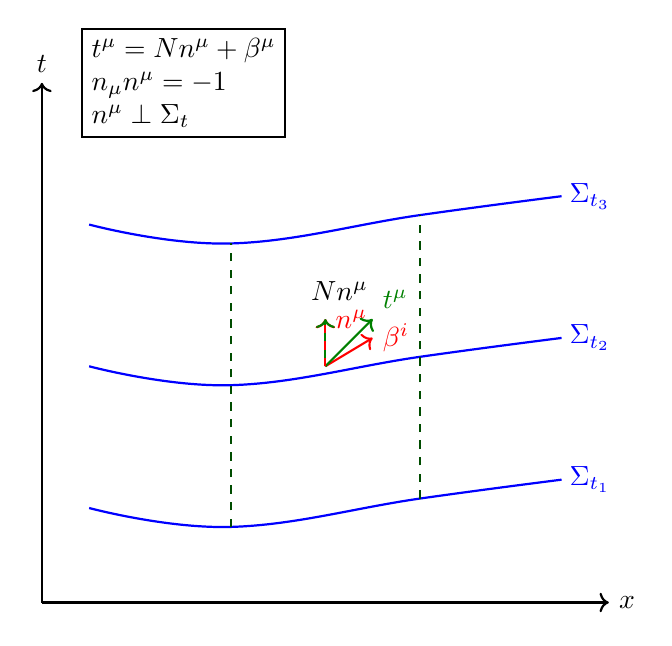
\begin{tikzpicture}[scale=1.2]
    % 坐标轴
    \draw[->,thick] (0,0) -- (6,0) node[right] {$x$};
    \draw[->,thick] (0,0) -- (0,5.5) node[above] {$t$};
    
    % 三张超曲面 \Sigma_{t1}, \Sigma_{t2}, \Sigma_{t3}
    \draw[blue,thick] plot[smooth,tension=0.7] coordinates {(0.5,1) (2,0.8) (4,1.1) (5.5,1.3)};
    \node[blue] at (5.8,1.3) {$\Sigma_{t_1}$};
    
    \draw[blue,thick] plot[smooth,tension=0.7] coordinates {(0.5,2.5) (2,2.3) (4,2.6) (5.5,2.8)};
    \node[blue] at (5.8,2.8) {$\Sigma_{t_2}$};
    
    \draw[blue,thick] plot[smooth,tension=0.7] coordinates {(0.5,4) (2,3.8) (4,4.1) (5.5,4.3)};
    \node[blue] at (5.8,4.3) {$\Sigma_{t_3}$};
    
    % 法向量 n (从 Sigma_{t2} 向上)
    \draw[red,->,thick] (3,2.5) -- (3,3.0) node[right] {$n^\mu$};
    \draw[red,->] (3,2.5) -- (3.5,2.8) node[right] {$\beta^i$};
    
    % 时间演化向量 t^mu
    \draw[->,thick,green!50!black] (3,2.5) -- (3.5,3.0) node[above right] {$t^\mu$};
    \draw[green!50!black,->] (3,2.5) -- (3,3.0);
    
    % 标注 N n
    \draw[red,dashed] (3,2.5) -- (3,3.0);
    \node at (3.15,3.3) {$N n^\mu$};
    
    % 世界线
    \draw[green!30!black,dashed] (2,0.8) -- (2,2.3) -- (2,3.8);
    \draw[green!30!black,dashed] (4,1.1) -- (4,2.6) -- (4,4.1);
    
    % 图例
    \node[draw,fill=white,align=left] at (1.5,5.5) {
        $t^\mu = N n^\mu + \beta^\mu$\\
        $n_\mu n^\mu = -1$\\
        $n^\mu \perp \Sigma_t$
    };
\end{tikzpicture}
\caption{3+1 分解的几何图示。时空被类空超曲面 $\Sigma_t$ 叶层化。$n^\mu$ 是 $\Sigma_t$ 的单位类时法向量。时间演化矢量 $t^\mu$ 分解为法向部分（lapse $N n^\mu$）和切向部分（shift $\beta^\mu$）。}
\label{fig:foliation}
\end{figure}

\subsection{Lapse 与 Shift}

叶层化引入了两个关键的运动学量：

\begin{definition}[Lapse 函数 $N$ 与 Shift 矢量 $\beta^i$]
设 $t^\mu = (\pd_t)^\mu$ 是坐标时间演化矢量。将 $t^\mu$ 相对于 $\Sigma_t$ 的法方向和切方向分解：
\begin{equation}
    \boxed{t^\mu = N n^\mu + \beta^\mu},
    \label{eq:lapse_shift_def}
\end{equation}
其中 $n^\mu$ 是 $\Sigma_t$ 的单位类时法向量（$n_\mu n^\mu = -1$），$\beta^\mu$ 是切向矢量（$\beta^\mu n_\mu = 0$），其空间分量记为 $\beta^i$。$N$ 称为\textbf{lapse 函数}，$\beta^i$ 称为\textbf{shift 矢量}。
\label{def:lapse_shift}
\end{definition}

Lapse 函数 $N$ 的物理含义：在相邻的两张时间切片之间，从一个切片上某一点出发，沿法向量 $n^\mu$ 方向行进的\textbf{固有时间}为 $\dd\tau = N \dd t$。因此 $N$ 描述了“时间流逝的速率”。

Shift 矢量 $\beta^i$ 的物理含义：它描述了空间坐标从一张切片到下一张切片时的“滑动”——即坐标系在空间方向上的漂移。

\subsection{四维度规的分解}

有了 lapse 和 shift，四维度规 $g_{\mu\nu}$ 可以用空间度规 $\gamma_{ij}$ 表示：

\begin{theorem}[ADM 度规分解]
在 3+1 分解下，四维线元写为：
\begin{equation}
    \boxed{\dd s^2 = -N^2 \dd t^2 + \gamma_{ij}(\dd x^i + \beta^i \dd t)(\dd x^j + \beta^j \dd t)}.
    \label{eq:ADM_line_element}
\end{equation}
或者等价地，四维度规及其逆为：
\begin{align}
    g_{\mu\nu} &= \begin{pmatrix}
        -N^2 + \beta_k\beta^k & \beta_i \\
        \beta_j & \gamma_{ij}
    \end{pmatrix},
    \label{eq:ADM_metric_matrix}
    \\[4pt]
    g^{\mu\nu} &= \begin{pmatrix}
        -1/N^2 & \beta^i/N^2 \\[2pt]
        \beta^j/N^2 & \gamma^{ij} - \beta^i\beta^j/N^2
    \end{pmatrix},
    \label{eq:ADM_inverse_metric}
\end{align}
其中 $\beta_i = \gamma_{ij}\beta^j$，$\beta_k\beta^k = \gamma_{ij}\beta^i\beta^j$。
\label{thm:ADM_metric}
\end{theorem}

\begin{proof}[推导]
由 $t^\mu = N n^\mu + \beta^\mu$，且 $n_\mu n^\mu = -1$，$n_\mu \beta^\mu = 0$。四维线元 $\dd s^2 = g_{\mu\nu}\dd x^\mu\dd x^\nu$，其中 $\dd x^0 = \dd t$。将坐标微分写为 $\dd x^\mu = t^\mu \dd t + (\dd x^\mu)_\perp$，其中 $(\dd x^\mu)_\perp$ 是 $\Sigma_t$ 上的切矢量。经过直接计算可得式 (\ref{eq:ADM_line_element})。详细推导见 \cite{Gourgoulhon2007}。
\end{proof}

\begin{note}[符号约定]
本书中，四维时空指标为希腊字母 ($\mu,\nu,\ldots=0,1,2,3$)，三维空间指标为拉丁字母 ($i,j,\ldots=1,2,3$)。空间度规 $\gamma_{ij}$ 是正定的。$\gamma^{ij}$ 是 $\gamma_{ij}$ 的逆：$\gamma^{ik}\gamma_{kj} = \delta^i_j$。
\end{note}

%=============================================================================
\section{诱导度规与外曲率}
\label{sec:induced_extrinsic}

\subsection{诱导度规 $\gamma_{ij}$}

类空超曲面 $\Sigma_t$ 从四维时空度规继承了一个\textbf{诱导度规}（induced metric）——也称为\textbf{第一基本形式}：

\begin{definition}[诱导度规 / 空间度规]
$\Sigma_t$ 上的诱导度规 $\gamma_{ij}$ 定义为四维度规 $g_{\mu\nu}$ 在 $\Sigma_t$ 上的限制：
\begin{equation}
    \boxed{\gamma_{ij} \equiv g_{\mu\nu} \, e^\mu_i \, e^\nu_j},
    \label{eq:gamma_def}
\end{equation}
其中 $e^\mu_i = \pd x^\mu / \pd y^i$ 是将 $\Sigma_t$ 上的坐标 $y^i$ 映射到时空坐标 $x^\mu$ 的切映射。在实际计算中，通常取 $y^i = x^i$（空间坐标），此时 $\gamma_{ij}$ 恰好就是四维度规的空间分量。
\end{definition}

度规 $\gamma_{ij}$ 的协变导数记为 $D_i$（与四维协变导数 $\nabla_\mu$ 区分）。相应的三维 Christoffel 符号为：
\begin{equation}
    \Gamma^i_{jk} = \frac{1}{2}\gamma^{i\ell}(\pd_j\gamma_{k\ell} + \pd_k\gamma_{j\ell} - \pd_\ell\gamma_{jk}).
    \label{eq:Gamma3}
\end{equation}

\subsection{外曲率 $K_{ij}$}

除了度规，$\Sigma_t$ 作为嵌入在四维时空中的超曲面还有第二个基本微分几何量——\textbf{外曲率}（extrinsic curvature，第二基本形式）：

\begin{definition}[外曲率]
$\Sigma_t$ 的外曲率 $K_{\mu\nu}$ 定义为法向量 $n^\mu$ 的协变导数在 $\Sigma_t$ 上的投影：
\begin{equation}
    \boxed{K_{\mu\nu} \equiv -\gamma^\rho_\mu \gamma^\sigma_\nu \nabla_\rho n_\sigma}.
    \label{eq:K_def}
\end{equation}
其中 $\gamma^\mu_\nu = \delta^\mu_\nu + n^\mu n_\nu$ 是投影到 $\Sigma_t$ 上的投影算子。外曲率的空间分量记为 $K_{ij}$。
\label{def:extrinsic_curvature}
\end{definition}

外曲率也可以理解为法向量沿 $\Sigma_t$ 的 Lie 导数的负数：
\begin{equation}
    K_{ij} = -\frac{1}{2}\Lie_n \gamma_{ij},
    \label{eq:K_Lie}
\end{equation}
其中 $\Lie_n$ 是沿法向量 $n^\mu$ 的李导数。由此得到 $K_{ij}$ 的运动学表达式：
\begin{equation}
    \boxed{K_{ij} = \frac{1}{2N}\left(D_i\beta_j + D_j\beta_i - \pd_t\gamma_{ij}\right)}.
    \label{eq:K_kinematic}
\end{equation}

\begin{property}[外曲率的物理含义]
    \begin{enumerate}
        \item 外曲率描述 $\Sigma_t$ 如何嵌入在四维时空中的“弯曲程度”——即法向量沿超曲面的变化率。
        \item $K_{ij} = 0$ 意味着超曲面是“全测地的”（totally geodesic），即法向量沿超曲面保持不变。
        \item 迹 $K = \gamma^{ij}K_{ij}$ 称为\textbf{平均曲率}，描述空间体积元的膨胀率：$\dd V / \dd\tau = -K \dd V$。
        \item 在宇宙学中，$K = -3H$（Hubble 参数），负号源于我们的符号约定。
    \end{enumerate}
\end{property}

\subsection{Gauss--Codazzi 关系}

四维时空的曲率与三维超曲面上的几何量通过 Gauss--Codazzi 方程相关联：

\begin{theorem}[Gauss--Codazzi 方程]
四维 Riemann 张量 $R^\mu_{\nu\rho\sigma}$ 在 $\Sigma_t$ 上的投影可以分解为：
\begin{align}
    \boxed{\gamma^\mu_\alpha \gamma^\beta_\nu \gamma^\rho_\gamma \gamma^\sigma_\delta \, R^\alpha_{\beta\rho\sigma} = {}^{(3)}\!R^\mu_{\nu\gamma\delta} + K^\mu_\gamma K_{\nu\delta} - K^\mu_\delta K_{\nu\gamma}},
    \label{eq:Gauss}
\end{align}
这是\textbf{Gauss 方程}，其中 ${}^{(3)}\!R^\mu_{\nu\gamma\delta}$ 是由 $\gamma_{ij}$ 计算的三维 Riemann 张量。

\textbf{Codazzi 方程}将 Ricci 张量的混合投影与外曲率的三维协变导数相联系：
\begin{equation}
    \boxed{\gamma^\mu_\alpha \gamma^\rho_\beta n^\sigma \, R_{\mu\rho\nu\sigma} = D_\beta K_{\alpha\nu} - D_\alpha K_{\beta\nu}}.
    \label{eq:Codazzi}
\end{equation}
\label{thm:Gauss_Codazzi}
\end{theorem}

这些关系是将四维 Einstein 方程分解为约束方程和演化方程的关键工具。详细的推导可参阅 \cite{Gourgoulhon2007,Wald1984}。

%=============================================================================
\section{ADM 演化方程与约束方程}
\label{sec:ADM_evolution_constraints}

\subsection{约束方程}

将 Gauss--Codazzi 关系代入 Einstein 方程，可以得到两组不与时间导数有关的方程——即每张空间切片上都必须满足的\textbf{约束方程}（constraint equations）：

\begin{theorem}[Hamilton 约束方程]
由 Einstein 方程的 $G_{\mu\nu}n^\mu n^\nu = \frac{8\pi G}{c^4} T_{\mu\nu}n^\mu n^\nu$ 得到：
\begin{equation}
    \boxed{{}^{(3)}\!R + K^2 - K_{ij}K^{ij} = \frac{16\pi G}{c^4} \rho},
    \label{eq:Hamiltonian_constraint}
\end{equation}
其中 ${}^{(3)}\!R$ 是由 $\gamma_{ij}$ 计算的三维 Ricci 标量，$K = \gamma^{ij}K_{ij}$ 是平均曲率，$\rho \equiv T_{\mu\nu}n^\mu n^\nu$ 是 Euler 观测者测得的能量密度。
\label{thm:Hamiltonian_constraint}
\end{theorem}

\begin{theorem}[动量约束方程]
由 Einstein 方程的混合投影 $G_{\mu\nu}\gamma^\mu_\alpha n^\nu = \frac{8\pi G}{c^4} T_{\mu\nu}\gamma^\mu_\alpha n^\nu$ 得到：
\begin{equation}
    \boxed{D_j(K^{ij} - \gamma^{ij}K) = \frac{8\pi G}{c^4} j^i},
    \label{eq:momentum_constraint}
\end{equation}
其中 $j^i \equiv -T_{\mu\nu}\gamma^{i\mu}n^\nu$ 是动量密度。
\label{thm:momentum_constraint}
\end{theorem}

在真空中（$\rho=0, j^i=0$），约束方程简化为：
\begin{align}
    {}^{(3)}\!R + K^2 - K_{ij}K^{ij} &= 0, \label{eq:vacuum_Hamiltonian} \\
    D_j(K^{ij} - \gamma^{ij}K) &= 0. \label{eq:vacuum_momentum}
\end{align}

\begin{note}[约束方程的角色]
    约束方程不包含 $\gamma_{ij}$ 或 $K_{ij}$ 的时间导数——它们必须在\textbf{初始数据}上精确满足。如果初始数据满足约束，则演化方程保证约束在以后的各个时刻自动满足（这是 Bianchi 恒等式的结果）。在数值计算中，约束违反的增长是衡量数值精度的重要指标。
\end{note}

\subsection{演化方程}

$\gamma_{ij}$ 和 $K_{ij}$ 的时间演化由以下方程控制：

\begin{theorem}[ADM 演化方程]
空间度规的演化方程（本质上是 $K_{ij}$ 的定义式）：
\begin{equation}
    \boxed{\pd_t \gamma_{ij} = -2N K_{ij} + D_i\beta_j + D_j\beta_i}.
    \label{eq:ADM_evol_gamma}
\end{equation}

外曲率的演化方程（由 Einstein 方程的空间投影得到）：
\begin{equation}
    \boxed{\begin{aligned}
        \pd_t K_{ij} &= N\bigl({}^{(3)}\!R_{ij} - 2K_{ik}K^k_j + K K_{ij}\bigr) - D_i D_j N \\
        &\quad + \beta^k D_k K_{ij} + K_{ik}D_j\beta^k + K_{kj}D_i\beta^k \\
        &\quad - 4\pi G N\bigl(2S_{ij} - \gamma_{ij}(S - \rho)\bigr).
    \end{aligned}}
    \label{eq:ADM_evol_K}
\end{equation}
其中 $S_{ij} \equiv T_{\mu\nu}\gamma^\mu_i\gamma^\nu_j$ 是空间应力张量，$S = \gamma^{ij}S_{ij}$ 是其迹。
\label{thm:ADM_evolution}
\end{theorem}

完整的 ADM 动力学系统包括：六个 $\gamma_{ij}$ 演化方程、六个 $K_{ij}$ 演化方程，加上 Hamilton 约束和三个动量约束——一共是十二个演化变量和四个约束。Lapse $N$ 和 shift $\beta^i$ 不是动力学变量，而是\textbf{规范自由度}，可以自由选择（对应坐标条件的选取）。

\begin{note}[ADM 形式的数值困境]
    尽管 ADM 形式在理论上优雅完备，但在实际数值模拟中表现出严重的\textbf{数值不稳定性}。其根本原因在于 ADM 方程系统不是强双曲的（strongly hyperbolic），微小的高频噪声会在演化过程中迅速增长。这一难题直到 1990 年代 BSSN 重新构造演化方程后才得以解决。
\end{note}

%=============================================================================
\section{BSSN 形式}
\label{sec:BSSN}

由于 ADM 形式的数值不稳定性，Baumgarte、Shapiro、Shibata 和 Nakamura 在 1990 年代提出了一种重新构造的演化系统——\textbf{BSSN 形式}，现在已成为数值相对论的主流方案。

\subsection{共形分解}

BSSN 形式的核心思想是将空间度规进行共形分解：

\begin{definition}[BSSN 变数]
引入共形因子 $\phi$ 或 $\chi$，将空间度规分解为：
\begin{equation}
    \boxed{\gamma_{ij} = e^{4\phi} \tilde{\gamma}_{ij} \quad\text{或}\quad \gamma_{ij} = \chi^{-1}\tilde{\gamma}_{ij}},
    \label{eq:conformal_decomp}
\end{equation}
其中 $\tilde{\gamma}_{ij}$ 是\textbf{共形度规}，其行列式被固定（通常取 $\det\tilde{\gamma}_{ij} = 1$，从而 $\chi = (\det\gamma_{ij})^{-1/3} = e^{-4\phi}$）。

外曲率分解为迹部分和无迹部分：
\begin{align}
    K &= \gamma^{ij}K_{ij}, \label{eq:trace_K} \\
    \tilde{A}_{ij} &\equiv e^{-4\phi}\left(K_{ij} - \frac{1}{3}\gamma_{ij}K\right),
    \label{eq:Atilde_def}
\end{align}
使得 $\tilde{A}_{ij}$ 对共形度规无迹：$\tilde{\gamma}^{ij}\tilde{A}_{ij} = 0$。
\label{def:BSSN_variables}
\end{definition}

此外，引入\textbf{共形联络函数}（conformal connection functions）：
\begin{equation}
    \boxed{\tilde{\Gamma}^i \equiv \tilde{\gamma}^{jk}\tilde{\Gamma}^i_{jk} = -\pd_j \tilde{\gamma}^{ij}},
    \label{eq:Gamma_conformal}
\end{equation}
其中 $\tilde{\Gamma}^i_{jk}$ 是由共形度规 $\tilde{\gamma}_{ij}$ 计算的 Christoffel 符号。$\tilde{\Gamma}^i$ 在 BSSN 中被提升为独立的演化变量，这是使系统强双曲的关键步骤。

\subsection{BSSN 演化方程}

BSSN 系统的完整演化方程如下（真空中，$c=1, G=1$）：

\begin{theorem}[BSSN 演化系统]
\textbf{共形因子：}
\begin{equation}
    \pd_t \phi = -\frac{1}{6}N K + \beta^i\pd_i\phi + \frac{1}{6}\pd_i\beta^i.
    \label{eq:BSSN_phi}
\end{equation}

\textbf{共形度规：}
\begin{equation}
    \pd_t \tilde{\gamma}_{ij} = -2N\tilde{A}_{ij} + \beta^k\pd_k\tilde{\gamma}_{ij} + \tilde{\gamma}_{ik}\pd_j\beta^k + \tilde{\gamma}_{kj}\pd_i\beta^k - \frac{2}{3}\tilde{\gamma}_{ij}\pd_k\beta^k.
    \label{eq:BSSN_gammatilde}
\end{equation}

\textbf{外曲率迹：}
\begin{equation}
    \pd_t K = -\gamma^{ij}D_i D_j N + N\left(\tilde{A}_{ij}\tilde{A}^{ij} + \frac{1}{3}K^2\right) + \beta^i\pd_i K.
    \label{eq:BSSN_K}
\end{equation}

\textbf{无迹外曲率：}
\begin{equation}
    \begin{aligned}
        \pd_t \tilde{A}_{ij} &= e^{-4\phi}\Bigl[-D_i D_j N + N\,{}^{(3)}\!R_{ij}\Bigr]^{\text{TF}} \\
        &\quad + N\left(K\tilde{A}_{ij} - 2\tilde{A}_{ik}\tilde{A}^k_j\right) \\
        &\quad + \beta^k\pd_k\tilde{A}_{ij} + \tilde{A}_{ik}\pd_j\beta^k + \tilde{A}_{kj}\pd_i\beta^k - \frac{2}{3}\tilde{A}_{ij}\pd_k\beta^k,
    \end{aligned}
    \label{eq:BSSN_Atilde}
\end{equation}
其中 $[\cdots]^{\text{TF}}$ 表示取无迹部分。

\textbf{共形联络函数：}
\begin{equation}
    \begin{aligned}
        \pd_t \tilde{\Gamma}^i &= -2\tilde{A}^{ij}\pd_j N + 2N\Bigl(\tilde{\Gamma}^i_{jk}\tilde{A}^{kj} - \frac{2}{3}\tilde{\gamma}^{ij}\pd_j K\Bigr) \\
        &\quad + \beta^j\pd_j\tilde{\Gamma}^i - \tilde{\Gamma}^j\pd_j\beta^i + \frac{2}{3}\tilde{\Gamma}^i\pd_j\beta^j + \tilde{\gamma}^{jk}\pd_j\pd_k\beta^i.
    \end{aligned}
    \label{eq:BSSN_Gamma}
\end{equation}
\label{thm:BSSN_system}
\end{theorem}

\begin{property}[BSSN vs ADM]
    BSSN 系统相比 ADM 的优越之处：
    \begin{enumerate}
        \item \textbf{强双曲性}：将 $\tilde{\Gamma}^i$ 提升为独立变量后，演化系统的主部具有强双曲结构，保证适定性（well-posedness）。
        \item \textbf{约束传播}：约束方程（Hamilton 和动量约束）的违反在 BSSN 中不会自发增长——系统具有“约束阻尼”性质。
        \item \textbf{共形分解}：将体积因子（共形因子 $\phi$ 或 $\chi$）与形状（共形度规 $\tilde{\gamma}_{ij}$）分离，使奇点附近的数值行为更可控。
    \end{enumerate}
\end{property}

\subsection{规范条件}

Lapse 和 shift 的选择（即\textbf{切片条件}和\textbf{空间坐标条件}）对数值模拟的稳定性和物理结果至关重要。BSSN 常用的规范条件有：

\begin{definition}[1+log 切片条件]
\begin{equation}
    \boxed{\pd_t N = \beta^i \pd_i N - 2 N K}.
    \label{eq:one_plus_log}
\end{equation}
这个条件使得 $N$ 沿法向量的 Lie 导数为 $\Lie_n N = -2K$。在 $K>0$（坍缩）区域，$N$ 减小（时间“冻结”），这对黑洞奇点附近的模拟极其有利——称为\textbf{奇点避免切片}（singularity-avoiding slicing）。
\label{def:one_plus_log}
\end{definition}

\begin{definition}[Gamma-driver 条件]
Shift 矢量 $\beta^i$ 的演化通常由\textbf{Gamma-driver} 条件控制：
\begin{align}
    \pd_t \beta^i &= \frac{3}{4} B^i, \label{eq:gamma_driver1} \\
    \pd_t B^i &= \pd_t \tilde{\Gamma}^i - \eta B^i,
    \label{eq:gamma_driver2}
\end{align}
其中 $\eta$ 是阻尼参数（典型的取值 $\eta \sim 1/(2M)$）。这个条件使 $\tilde{\Gamma}^i$ 趋近于零，从而保持空间坐标的“最小畸变”状态。
\label{def:gamma_driver}
\end{definition}

\begin{note}[移动 puncture 方法]
1+log 切片与 Gamma-driver 条件的组合构成了著名的\textbf{移动 puncture 方法}（moving puncture method）的核心。这一方法不需要对黑洞内部进行特殊的奇点切除（excision），而是在奇点附近自然地“冻结”演化，使数值模拟能够稳定地穿越视界。搭配 BSSN 演化系统，移动 puncture 方法是目前应用最广泛的黑洞并合数值方案。
\end{note}

%=============================================================================
\section{黑洞模拟中的奇点处理}
\label{sec:singularity_treatment}

黑洞时空中存在物理奇点（曲率发散处）。如何在数值模拟中处理奇点而不使计算崩溃，是数值相对论中的核心工程问题。有三种主要策略：

\subsection{Puncture 方法}

Puncture 方法是处理黑洞初始数据的一种技术。

\begin{definition}[Puncture 初始数据]
在 Brill--Lindquist 类型的初始数据中，黑洞由 Schwarzschild 时空的 Einstein--Rosen 桥（wormhole）的“喉咙”表示。通过共形分解，在坐标奇点（puncture）附近，共形因子以 $\phi \sim \ln r$（或 $\chi \sim r^2$）的行为发散。在数值网格上，这些 puncture 点被处理为坐标奇点——共形因子在 puncture 处被正则化，而度规的物理奇异性被隐藏在 puncture 背后。
\label{def:puncture}
\end{definition}

Puncture 方法的关键是：黑洞的视界位于 puncture 之外，因此在视界外部，所有几何量都是正则的。在视界内部，虽然存在坐标奇点，但它不会影响外部区域的演化。

\subsection{移动 puncture 方法}

这是 BSSN 系统常用的完整演化方案：

\begin{enumerate}
    \item \textbf{初始数据}：构造包含多个 puncture 的初始数据，每个 puncture 代表一个黑洞。
    \item \textbf{演化}：使用 BSSN 方程 + 1+log 切片 + Gamma-driver 条件进行全三维演化。Puncture 点在演化中会自由移动（因此称为“移动”puncture）。
    \item \textbf{奇点避免}：1+log 切片条件使 lapse 在黑洞内部迅速坍缩到零，从而在接近物理奇点的地方“冻结”坐标时间演化。
    \item \textbf{无需内部边界}：由于 lapse 坍缩，黑洞内部的演化被有效抑制，不需要在视界处设置内部边界条件（这与 excision 方法不同）。
\end{enumerate}

\begin{property}[移动 puncture 方法的优势]
    \begin{itemize}
        \item 实现简单——不需要复杂的内部边界条件。
        \item 稳健——对多个黑洞的轨道动力学非常鲁棒。
        \item 自动处理并合——两个 puncture 自然并合为一个。
    \end{itemize}
\end{property}

\subsection{Excision 方法}

Excision（切除）方法是一种更直接但技术更复杂的方法：

\begin{definition}[Excision]
在演化过程中，Black hole interior（视界内部）的网格点被主动从计算域中“切除”。在视界表面施加出射边界条件（outgoing boundary condition），确保没有任何信息从内部传播到外部。因为视界是单向膜（one-way membrane），外部的物理演化完全独立于内部。
\label{def:excision}
\end{definition}

Excision 方法的挑战在于：需要实时追踪视界的位置（通常通过求解视界寻找方程），并在移动的视界表面施加合适的边界条件。这对复杂并合过程（如双黑洞并合中视界的剧烈变形和合并）提出了巨大的技术挑战。

\begin{note}[两种方法的现状]
    目前，移动 puncture 方法因其实现简单和稳健性，已成为双黑洞并合模拟的主流方案。Excision 方法在某些高精度场景（如需要长时间精确演化的极端质量比旋近 EMRI 模拟）中仍有应用，但总体使用较少。广义调和坐标（generalized harmonic coordinates）方法是第三种流行的选择，被 SpEC (SXS) 合作组广泛使用。
\end{note}

%=============================================================================
\section{引力波形提取}
\label{sec:waveform_extraction}

数值模拟的最终“产品”是引力波信号。从数值时空度规中提取引力波形需要特殊的数学技术。

\subsection{Newman--Penrose 标量 $\Psi_4$}

在弱场区域（远离源），引力波信息由 Weyl 张量的分量携带。Newman--Penrose (NP) 形式提供了一个方便的标架形式来提取它：

\begin{definition}[$\Psi_4$ 标量]
Weyl 张量 $C_{\mu\nu\rho\sigma}$ 的 NP 标量 $\Psi_4$ 定义为：
\begin{equation}
    \boxed{\Psi_4 \equiv C_{\mu\nu\rho\sigma} \, k^\mu \bar{m}^\nu k^\rho \bar{m}^\sigma},
    \label{eq:Psi4_def}
\end{equation}
其中 $\{k^\mu, \ell^\mu, m^\mu, \bar{m}^\mu\}$ 是 Newman--Penrose 类光标架。$k^\mu$ 是指向未来的外向类光矢量，$m^\mu$ 是复类空矢量。$\Psi_4$ 直接关联于引力波的两个偏振态：
\begin{equation}
    \boxed{\Psi_4 = \ddot{h}_+ - i\,\ddot{h}_\times},
    \label{eq:Psi4_waveform}
\end{equation}
其中 $h_+$ 和 $h_\times$ 分别是 plus 和 cross 偏振的引力波应变。
\label{def:Psi4}
\end{definition}

在数值计算中，需要首先在球壳上构造 NP 类光标架：
\begin{align}
    k^\mu &= \frac{1}{\sqrt{2}}(n^\mu + e^\mu_r), \quad
    \ell^\mu = \frac{1}{\sqrt{2}}(n^\mu - e^\mu_r), \\
    m^\mu &= \frac{1}{\sqrt{2}}(e^\mu_\theta + i\,e^\mu_\phi),
\end{align}
其中 $e^\mu_r, e^\mu_\theta, e^\mu_\phi$ 是以模拟中心为原点的球坐标基矢量。

\subsection{有限半径提取与外推}

在实际模拟中，$\Psi_4$ 在有限坐标半径 $r_{\text{ext}}$ 处计算（而非 $r \to \infty$）。为了获得等效于无穷远处探测器接收到的波形，需要进行外推。

\begin{example}[有限半径修正]
$\Psi_4$ 的大半径展开为：
\begin{equation}
    \Psi_4(t, r) = \frac{\Psi_4^{(0)}(t_{\text{ret}})}{r} + \Order(r^{-2}),
    \label{eq:Psi4_expansion}
\end{equation}
其中 $t_{\text{ret}} = t - r$ 是延迟时间。通过在不同半径 $r_1, r_2, \ldots, r_N$ 处提取波形，并拟合 $1/r$ 衰减律，可以外推得到 $r \to \infty$ 的波形：
\begin{equation}
    r\Psi_4(t, r) \big|_{r\to\infty} = \lim_{r\to\infty} r\,\Psi_4(t_{\text{ret}} + r, r).
\end{equation}
\end{example}

提取到的 $\Psi_4$ 需要经过两次时间积分才能得到引力波应变 $h(t)$。积分常数（由初始条件和低频噪声决定）是主要的误差源之一——这被称为\textbf{波形后处理中的漂移问题}。

\subsection{其他波形提取方法}

除 $\Psi_4$ 方法外，还有：
\begin{itemize}
    \item \textbf{Regge--Wheeler--Zerilli 扰动理论}：在 Schwarzschild 背景上将度规扰动分解为奇宇称和偶宇称部分。
    \item \textbf{Cauchy-characteristic extraction (CCE)}：将三维类空 Cauchy 数据通过特征演化传播到类光无穷远 $\mathcal{J}^+$，是获取精确渐近波形的最严格方法。
\end{itemize}

%=============================================================================
\section{算例：简单波动传播的数值模拟}
\label{sec:example}

作为数值相对论的人门示例，我们考虑平坦时空中标量波的传播——这是一个简化的但包含许多数值相对论关键技术的模型。

\subsection{一维波动方程的有限差分解}

考虑一维波动方程：
\begin{equation}
    \pd_t^2 u - \pd_x^2 u = 0,
    \label{eq:wave1d}
\end{equation}
其中 $u(t,x)$ 是标量场。将其写为一阶形式（与 BSSN 系统的一阶约化类似）：
\begin{align}
    \pd_t u &= v, \label{eq:wave1d_u} \\
    \pd_t v &= \pd_x^2 u. \label{eq:wave1d_v}
\end{align}

使用二阶精度的中心差分格式进行空间离散。在均匀网格 $x_i = i\Delta x$ 上：
\begin{align}
    u_i^{n+1} &= u_i^n + \Delta t \, v_i^n, \\
    v_i^{n+1} &= v_i^n + \frac{\Delta t}{\Delta x^2}(u_{i+1}^n - 2u_i^n + u_{i-1}^n).
\end{align}

\begin{note}[CFL 条件]
该显式格式的稳定性要求满足 Courant--Friedrichs--Lewy (CFL) 条件：
\begin{equation}
    \Delta t \leq C \,\Delta x,
    \label{eq:CFL}
\end{equation}
其中 $C \leq 1$（对于一维波动方程，声速 $c_s=1$）。在数值相对论中，BSSN 系统使用的 CFL 因子通常取 $0.25$--$0.5$。
\end{note}

\subsection{代码结构示意}

下面给出该算例的完整 Python 代码示意（实际数值相对论代码如 BAM、Einstein Toolkit 用 C++/Fortran 编写并大规模并行化）：

\begin{verbatim}
import numpy as np
import matplotlib.pyplot as plt

# 参数
L = 10.0       # 计算域长度 [-L, L]
Nx = 200       # 网格点数
dx = 2*L / Nx
dt = 0.5 * dx  # CFL = 0.5
T = 8.0        # 总演化时间

# 网格
x = np.linspace(-L+dx/2, L-dx/2, Nx)

# 初始数据：高斯脉冲
u = np.exp(-x**2)
v = np.zeros_like(u)

# 时间演化
t = 0.0
while t < T:
    u_new = u + dt * v
    v_new = v + dt * (np.roll(u,1) - 2*u + np.roll(u,-1)) / dx**2
    u, v = u_new, v_new
    t += dt
\end{verbatim}

\begin{example}[结果分析]
该程序模拟了高斯脉冲分裂为向左和向右传播的两个波包。在每个时刻，总能量
\begin{equation}
    E(t) = \frac{1}{2}\int \bigl(v^2 + (\pd_x u)^2\bigr)\,\dd x
\end{equation}
应当是守恒的（准确说，在连续极限下守恒）。数值能量的漂移量是衡量有限差分格式精度的重要诊断指标。
\end{example}

这个简单示例体现了数值相对论的几个关键要素：（1）将二阶方程化为一阶系统；（2）选择合适的有限差分格式；（3）满足 CFL 稳定性条件；（4）用守恒量监控数值精度。实际的 BSSN 代码在这些基础上增加了共形分解、规范条件、自适应网格细化（AMR）以及大规模并行计算等复杂技术。

%=============================================================================

\begin{note}[进一步阅读]
数值相对论是一门仍在快速发展的交叉学科。对于希望深入了解的读者，推荐以下资源：
\begin{itemize}
    \item \cite{Gourgoulhon2007}：3+1 分解与数值方法的权威教科书。
    \item Baumgarte \& Shapiro (2010): \textit{Numerical Relativity: Solving Einstein's Equations on the Computer}，全面介绍 BSSN 系统和各种数值技术。
    \item Einstein Toolkit (\url{http://einsteintoolkit.org})：开源的数值相对论软件框架。
    \item SXS 合作组波形目录 (\url{https://www.black-holes.org/waveforms})：公开的数值波形数据库。
\end{itemize}
\end{note}
  % 数值相对论简介

%=============================================================================
% 第三部分：前沿专题
%=============================================================================

% chapter15.tex - AdS/CFT与量子引力
\chapter{AdS/CFT对偶与量子引力}
\label{chap:AdSCFT}

\section{量子引力的核心问题}

\begin{note}[物理动机]
量子引力是理论物理中最深远的未解决问题之一。它的根本困难在于：广义相对论和量子力学基于互不相容的数学框架。广义相对论是几何的、确定性的经典场论；量子力学是代数的、概率性的线性理论。将两者直接量化（即将度规视为量子场）会遇到不可重整化的紫外发散——微扰量子广义相对论在 Planck 能量以上丧失了预测能力。

AdS/CFT 对偶为这一困境提供了全新的出路：\textbf{不直接量化引力，而是用一个没有引力的量子场论来定义量子引力}。这正是全息原理的具体实现——引力系统等价于其边界上的非引力系统。在这个框架下，时空几何和引力本身变为\textbf{涌现}（emergent）的现象，而非基本的自由度 \cite{Maldacena1997,Witten1998,Maldacena2003}。
\end{note}

量子引力面临的核心问题包括：
\begin{enumerate}
    \item \textbf{黑洞信息悖论}：黑洞蒸发过程中信息是否丢失？量子幺正性如何与经典黑洞热力学相容？
    \item \textbf{时空奇点}：在 Planck 尺度上，时空的经典概念是否完全崩溃？量子效应如何抹平奇点？
    \item \textbf{全息原理}：引力系统的自由度是否本质上就是低维的？黑洞熵的面积律 $S = A/4G$ 暗示了什么？
    \item \textbf{时空的涌现}：时空几何是基本的还是从更底层的量子自由度中涌现的？
    \item \textbf{非微扰定义}：是否存在不依赖微扰展开的量子引力的完整定义？
\end{enumerate}

AdS/CFT 对偶对以上每一个问题都提供了原则性的答案或深刻的洞察。本章将从量子引力的视角出发，系统介绍这一对偶及其核心应用。主要参考文献包括 \cite{Maldacena1997,Witten1998,Gubser1998,Aharony1999,Nastase2007,Maldacena2003,Hubeny2015,Rangamani2016,Erdmenger2018}。

\section{AdS/CFT 对偶的表述}

\subsection{Maldacena 的发现与对偶的三种形式}

1997 年，Maldacena 提出 IIB 型超弦理论中 $N$ 张重合 D3-膜的低能极限存在两种等价描述 \cite{Maldacena1997}：开弦描述给出 $d=4$、$\mathcal{N}=4$ 超对称 $SU(N)$ Yang-Mills 理论（一个共形场论）；闭弦描述给出 $\mathrm{AdS}_5 \times S^5$ 上的 IIB 型超引力。

\begin{theorem}[AdS/CFT 对偶（三种形式）]
    \begin{enumerate}
        \item \textbf{最强形式}：IIB 型超弦在 $\mathrm{AdS}_5 \times S^5$ 上精确等价于 $d=4$、$\mathcal{N}=4$ $SU(N)$ SYM，对所有 $N$ 和 $g_{\text{YM}}$ 成立。
        \item \textbf{强形式}：取 $N \to \infty$ 且 $\lambda = g_{\text{YM}}^2 N$ 固定（平面极限），对偶为经典弦论在 $\mathrm{AdS}_5 \times S^5$ 上等价于大 $N$ 规范论的平面图求和。
        \item \textbf{弱形式（最常用）}：进一步取 $\lambda \to \infty$，对偶退化为 $d+1$ 维\textbf{经典引力}等价于 $d$ 维\textbf{强耦合大 $N$ 共形场论}。这正是量子引力最有用的极限：
        \begin{equation}
            \boxed{\text{经典引力} \;\Longleftrightarrow\; \text{强耦合大 $N$ CFT}}.
        \end{equation}
    \end{enumerate}
\end{theorem}

\begin{remark}[为什么这对量子引力重要]
    弱形式虽然只涉及经典引力，但它告诉我们：\textbf{即使引力量子效应（$1/N$ 修正）和有限弦长效应（$1/\lambda$ 修正）都不可忽略，边界 CFT 仍然是有明确定义的}。因此，边界上普通的量子场论为全体量子引力（包括所有弦修正和非微扰效应）提供了一个\textbf{非微扰的完整定义}。在这个意义上：\textbf{AdS/CFT 对偶是一个量子引力的定义}，而非仅仅是一个对偶关系。
\end{remark}

\subsection{参数对应与全息字典}

对偶两边的基本参数对应：
\begin{align}
    \frac{L^4}{\alpha'^2} &= 2\lambda = 2g_{\text{YM}}^2 N, \\
    \frac{L^4}{G_N} &= \frac{2N^2}{\pi}.
\end{align}
其中 $L$ 是 AdS 半径，$\alpha'$ 是弦张力倒数，$G_N$ 是 $d+1$ 维 Newton 常数。当 $N \to \infty$（大 $N$ 极限），体引力的量子涨落被抑制（$G_N \propto 1/N^2$）；当 $\lambda \to \infty$，弦的有限长度效应被抑制（$\alpha' \ll L^2$），引力退化为局域场论。

\section{AdS 时空的几何结构}

全息对偶的体时空是反德西特空间。从量子引力的角度看，AdS 时空最关键的几何性质是：\textbf{它具有一个类时的共形边界，信息可以从边界流入和流出体时空}——这使得引力的全息描述成为可能。

\begin{definition}[AdS$_{d+1}$ 的 Poincaré 度规]
    在 Poincaré 坐标下，AdS$_{d+1}$ 度规为：
    \begin{equation}
        \boxed{\dd s^2 = \frac{L^2}{z^2}\left(\dd z^2 + \eta_{\mu\nu}\dd x^\mu \dd x^\nu\right)},
    \end{equation}
    其中 $z \in (0,\infty)$ 为全息径向坐标，$z \to 0$ 对应共形边界（CFT 所在处），$z \to \infty$ 对应 Poincaré 视界。度规在 $z \to 0$ 处有一个二阶极点，提取共形因子 $L^2/z^2$ 后，边界度规为 $d$ 维 Minkowski 度规。
\end{definition}

\begin{theorem}[等距群-共形群对应]
    $\mathrm{AdS}_{d+1}$ 的等距群 $SO(2,d)$ 与其 $d$ 维共形边界的共形群精确同构。这是一切全息对偶的几何基础：\textbf{体时空的对称性 = 边界理论的对称性}。
\end{theorem}

\begin{remark}[UV/IR 对应：量子引力中的标度-几何对偶]
    全息对偶中最深刻的几何事实之一是\textbf{UV/IR 对应}：边界理论中短距离（高能、紫外）的物理对应于体时空中靠近边界（$z$ 小）的区域；长距离（低能、红外）的物理对应于体时空深处（$z$ 大）的区域。用公式表达：
    \begin{equation}
        z \sim \frac{1}{E_{\text{CFT}}}.
    \end{equation}
    这意味着：\textbf{边界量子场论的能标对应于体时空的几何深度}。在量子引力中，这一对偶意味着 Planck 尺度的几何可能由边界理论的远红外物理描述——这是一个令人震惊的颠倒。
\end{remark}

\section{GKPW 关系：量子引力的全息定义}

\subsection{配分函数的等价性}

Gubser、Klebanov、Polyakov \cite{Gubser1998} 和 Witten \cite{Witten1998} 给出了 AdS/CFT 对偶的精确数学表述：

\begin{theorem}[GKPW 关系]
    $d$ 维 CFT 的配分函数（生成泛函）等于 $d+1$ 维 AdS 中量子引力的配分函数，其边界条件由源 $\phi_0$ 确定：
    \begin{equation}
        \boxed{Z_{\text{CFT}}[\phi_0] = \int_{\phi \to \phi_0} \mathcal{D}\phi \, e^{i S_{\text{gravity}}[\phi]} \underset{N \to \infty}{\approx} e^{i S_{\text{on-shell}}[\phi_0]}}.
    \end{equation}
    在经典引力极限（$N \to \infty, \lambda \to \infty$）下，路径积分由经典鞍点主导，退化为壳上作用量的指数。
\end{theorem}

\begin{note}[GKPW 关系作为量子引力的定义]
    GKPW 关系的真正威力在于：右侧的体引力路径积分原则上包含了所有量子引力效应——引力子的圈图、非微扰的时空拓扑涨落、甚至 wormhole 构型。如果我们不知道如何直接计算这个路径积分（实际上我们确实不知道），我们可以转而使用左侧——一个\textbf{完全良定义的、没有引力的量子场论}——来\textbf{定义}它。

    这正是 AdS/CFT 作为量子引力框架的本质：不直接构建量子引力，而是通过一个已知的量子场论来\textbf{非微扰地定义}量子引力。
\end{note}

\subsection{边界渐近行为与全息字典}

在 AdS$_{d+1}$ 中，质量 $m$ 的标量场 $\phi(z,x)$ 在 $z \to 0$ 处具有渐近展开：
\begin{equation}
    \phi(z,x) \sim \phi_0(x) \, z^{d-\Delta} + \langle\mathcal{O}(x)\rangle \, z^{\Delta},
\end{equation}
其中共形维数 $\Delta$ 由质量-维数关系确定：
\begin{equation}
    \boxed{m^2 L^2 = \Delta(\Delta - d)}.
\end{equation}

$\phi_0(x)$ 是 CFT 中耦合于算符 $\mathcal{O}$ 的\textbf{源}，而 $\langle\mathcal{O}(x)\rangle$ 是该算符的\textbf{真空期望值}。这是全息字典的核心规则：\textbf{体场在边界处的"慢衰减"模式对应源，"快衰减"模式对应响应}。

\section{全息纠缠熵与时空的涌现}

量子引力中最激进的思想或许是：\textbf{时空几何本身不是基本的——它从量子纠缠中涌现}。支持这一观点的最有力证据来自全息纠缠熵的研究 \cite{Rangamani2016}。

\subsection{Ryu-Takayanagi 公式}

\begin{theorem}[Ryu-Takayanagi 公式（2006）]
    在静态全息时空中，边界 CFT 的空间子区域 $A$ 的纠缠熵等于体时空中\textbf{极小曲面} $\gamma_A$ 的面积（以 $4G_N$ 为单位），该曲面锚定在 $\partial A$ 上且与 $A$ 同伦：
    \begin{equation}
        \boxed{S_A = \frac{\operatorname{Area}(\gamma_A)}{4G_N^{(d+1)}}}, \qquad \partial\gamma_A = \partial A.
    \end{equation}
\end{theorem}

\begin{figure}[htbp]
\centering
\begin{tikzpicture}[scale=1.5]
    \draw[very thick] (-3,0) -- (3,0);
    \node at (3.3,0) {$\partial\mathrm{AdS}$ (边界CFT)};
    \draw[red, very thick] (-1.2,0) -- (1.2,0);
    \node[red] at (0,0.15) {$A$};
    \fill[red] (-1.2,0) circle (0.05) node[below] {$\partial A$};
    \fill[red] (1.2,0) circle (0.05) node[below] {$\partial A$};
    \draw[green!50!black, very thick] (-1.2,0) .. controls (-0.8,-1.0) and (0.8,-1.0) .. (1.2,0);
    \node[green!50!black] at (0,-1.1) {$\gamma_A$（极小曲面）};
    \draw[->] (0,0) -- (0,-1.8) node[below] {$z$（体深度）};
    \draw[dashed, gray] (-1.2,0) -- (-1.2,-1.3);
    \draw[dashed, gray] (1.2,0) -- (1.2,-1.3);
    \node at (-2.5,-1.2) {$S_A = \dfrac{\mathrm{Area}(\gamma_A)}{4G_N}$};
\end{tikzpicture}
\caption{Ryu-Takayanagi 极小曲面。边界子区域 $A$ 的纠缠熵 $S_A$ 由深入体时空的极小曲面 $\gamma_A$ 的面积决定。这一公式将量子信息（纠缠熵）与时空几何（极小曲面面积）精确联系起来——纠缠是几何的"原料"。}
\label{fig:RT_surface}
\end{figure}

\begin{remark}[RT 公式的革命性意义]
    RT 公式值得反复品味，因为它将三个看似无关的领域联系在一起：
    \begin{itemize}
        \item \textbf{量子信息}：纠缠熵是量子力学中衡量纠缠的基本量
        \item \textbf{广义相对论}：极小曲面是微分几何中的经典概念
        \item \textbf{黑洞热力学}：面积除以 $4G$ 正是 Bekenstein-Hawking 熵公式
    \end{itemize}
    RT 公式暗示：\textbf{黑洞熵只是纠缠熵的一个特例}——视界是锚定在黑洞自身上的"极小曲面"。这也意味着：时空几何（由 Einstein 方程描述）的动力学可能完全由边界量子态的纠缠结构决定。
\end{remark}

\subsection{从纠缠到 Einstein 方程}

2014 年，van Raamsdonk、Jacobson 等人基于 RT 公式提出了一个惊人的假设：Einstein 方程可以从纠缠熵的物理中推导出来。基本思路是：在 AdS/CFT 框架下，边界 CFT 的纠缠熵满足强次可加性等量子信息不等式；将这些不等式翻译到体时空的几何语言中，竟然导出了线性化的 Einstein 方程。

更一般地，考虑边界上一个微小变形的纠缠熵变化 $\delta S_A$。RT 公式将其与 $\delta(\text{Area})$ 联系起来，而极小曲面的面积变分涉及体时空的曲率。Faulkner 等人（2014）证明：
\begin{equation}
    \delta S_A = \frac{1}{4G_N} \int_{\gamma_A} \delta g^{\mu\nu} \, G_{\mu\nu} \, \dd V + \cdots,
\end{equation}
即爱因斯坦张量自然地出现在纠缠熵的一阶变分中。纠缠熵满足的量子信息约束条件恰好等价于 Einstein 方程在线性阶的成立。这一结果深刻表明：\textbf{时空的引力动力学可能完全由边界量子态的纠缠结构编码}。

\section{黑洞信息悖论与岛公式}

\subsection{信息悖论的历史}

1974-1976 年，Hawking 证明黑洞会发射热辐射并最终完全蒸发 \cite{Hawking1974}。如果初始物质处于纯量子态，黑洞形成后最终只剩下热辐射——一个混合态。这违反了量子力学的幺正性原理（纯态只能演化为纯态）。这就是困扰理论物理四十余年的\textbf{黑洞信息悖论}。

AdS/CFT 对偶原则上保证幺正性：边界 CFT 的 Hamilton 演化是幺正的，因此体时空中一切过程——包括黑洞形成和蒸发——必须也是幺正的。但在 2019 年之前，无人能具体展示信息如何从黑洞中逃逸。

\subsection{量子极端曲面与岛公式}

2019-2020 年，Penington、Almheiri、Engelhardt、Marolf、Maxfield 等人取得了重大突破：他们发现了计算蒸发黑洞辐射熵的正确方法。

\begin{theorem}[量子极端曲面公式（岛公式）]
    在包含引力的系统中，辐射的纠缠熵由广义的 RT 公式给出：
    \begin{equation}
        \boxed{S_{\text{rad}} = \min_X \left\{\operatorname{ext}_X\left[\frac{\operatorname{Area}(X)}{4G_N} + S_{\text{bulk}}(\Sigma_X)\right]\right\}},
    \end{equation}
    其中 $X$ 是体时空中的一个曲面（称为\textbf{量子极端曲面}），而 $S_{\text{bulk}}(\Sigma_X)$ 是体量子场在区域 $\Sigma_X$ 中的纠缠熵。后一项包含了 Hawking 辐射中量子关联的贡献。

    关键的物理图像：在蒸发早期，极小曲面 $X$ 是\textbf{平凡曲面}（退化为边界截断），辐射熵由体量子场的熵主导，随辐射增加而增长。在蒸发后期（Page 时间之后），一个新的量子极端曲面出现在黑洞视界内部——即\textbf{岛}（island）——其面积贡献使总辐射熵开始下降。
\end{theorem}

\begin{remark}[Page 曲线与信息恢复]
    岛公式成功地再现了蒸发黑洞的 \textbf{Page 曲线}：
    \begin{itemize}
        \item $t < t_{\text{Page}}$：辐射熵从零线性增长至 $\sim$ 黑洞初始熵的一半。
        \item $t = t_{\text{Page}}$：Page 时间，辐射熵达到峰值，拐弯后开始下降。
        \item $t > t_{\text{Page}}$：辐射熵单调递减至零，意味着信息开始从黑洞中逸出——幺正性得以保持。
    \end{itemize}
    岛公式的关键发现是：在蒸发后期，黑洞内部出现了\textbf{纠缠岛}——辐射与岛内的量子态纠缠，导致辐射的熵降低。计算中必须将岛的贡献包含在内才能得到正确（幺正的）结果。这一发现标志着黑洞信息问题的实质性突破。
\end{remark}

\section{ER = EPR：纠缠就是几何}

\begin{theorem}[ER = EPR 猜想（Maldacena \& Susskind, 2013）]
    两个量子系统之间的\textbf{Einstein-Podolsky-Rosen (EPR) 纠缠}在几何上对偶于连接它们的\textbf{Einstein-Rosen (ER) 桥}（虫洞）：
    \begin{equation}
        \boxed{\text{纠缠} \;\Longleftrightarrow\; \text{时空连通性}}.
    \end{equation}
\end{theorem}

\subsection{猜想的证据}

ER = EPR 猜想并非凭空想象，它有多个层次的证据支持：

\begin{enumerate}
    \item \textbf{热场二重态与永恒 AdS 黑洞}：边界 CFT 的\textbf{热场二重态}（thermofield double state）是两个 CFT 之间的最大纠缠纯态。其对偶的体几何恰好是一个永恒 AdS-Schwarzschild 黑洞——它的两个渐近 AdS 区域通过一个不可穿越的 Einstein-Rosen 桥（虫洞）连接。纠缠越强，虫洞越长。
    
    \item \textbf{RT 公式的极限情况}：当 $A$ 是整个边界空间时，$S_A$ 是边界 CFT 的整体纠缠熵。RT 公式将其对偶于穿越整个体时空的极小曲面面积。当纠缠熵非零时，体时空的两个区域被"缝合"在一起——这正是虫洞的几何图像。
    
    \item \textbf{防火墙悖论的消解}：AMPS (2012) 提出的防火墙悖论声称：黑洞视界附近必须有一个高能"防火墙"才能满足量子力学的约束。ER = EPR 提供了一个优雅的解决方案：黑洞内部与早期 Hawking 辐射之间存在大量的纠缠（EPR），按照猜想，这对应于连接黑洞与辐射的虫洞（ER）。信息通过虫洞逃逸，无需引入任何奇异的防火墙。
\end{enumerate}

\begin{note}[量子引力的图像：时空作为纠缠的编织]
    如果 ER = EPR 猜想成立——越来越多的证据指向这一点——那么它将彻底改变我们对时空的理解：
    \begin{itemize}
        \item 经典时空中两个点之间的\textbf{连通性}是底层量子\textbf{纠缠}的宏观表现
        \item Einstein 方程 $G_{\mu\nu} = 8\pi G T_{\mu\nu}$ 可以理解为纠缠结构对物质分布的响应
        \item 量子引力中时空拓扑的涨落（包括虫洞的产生和湮灭）对偶于量子态的纠缠结构变化
        \item 时空的\textbf{涌现}意味着：在 Planck 尺度，时空概念分解为纯粹的量子信息结构
    \end{itemize}
\end{note}

\section{张量网络与纠缠构建时空}

\begin{definition}[MERA 张量网络]
    \textbf{多尺度纠缠重整化假设}（MERA）是一种用于表示量子多体系统基态的变分张量网络。它具有逐层构建的分层结构：每一层由\textbf{解纠缠器}（disentangler，消除局域冗余纠缠）和\textbf{等距映射}（isometry，进行粗粒化）组成。
\end{definition}

Swingle (2012) 发现 MERA 的结构与 AdS 时空的离散化有着精确的对应：
\begin{itemize}
    \item 网络的\textbf{层数} $\leftrightarrow$ AdS 的径向方向 $z$（标度方向，对应重整化群流）
    \item 每层的\textbf{空间节点数} $\leftrightarrow$ AdS 切片上的"空间体积"（越深层节点越少，对应越小的边界区域）
    \item 解纠缠器移除的\textbf{局域纠缠} $\leftrightarrow$ AdS 几何中的空间梯度
    \item 切割网络连接边界子区域的\textbf{最少键数} $\leftrightarrow$ 极小曲面 $\gamma_A$ 的"面积"
\end{itemize}

\begin{remark}[涌现时空的微观机制]
    张量网络模型提供了时空涌现的一个\textbf{具体微观实现}：
    \begin{enumerate}
        \item 边界上的量子态由张量网络编码
        \item 网络内部的连接结构定义了离散的几何
        \item 不同区域的纠缠决定了空间中的"距离"
        \item 粗粒化操作（沿网络向上走）定义了从 UV 到 IR 的重整化群流——即从边界进入体时空深处的运动
        \item 在连续极限下，网络的几何逼近 AdS 时空——Einstein 方程从张量网络的纠缠优化条件中涌现
    \end{enumerate}
    这为"时空从量子纠缠中涌现"提供了一个\textbf{构造性的原理证明}。
\end{remark}

\section{总结：AdS/CFT 对偶的量子引力遗产}

AdS/CFT 对偶已经深刻重塑了我们对量子引力的理解。以下是几条核心遗产：

\begin{enumerate}
    \item \textbf{量子引力的非微扰定义}：AdS/CFT 提供了第一个量子引力（在负宇宙学常数下）的完整非微扰定义。边界 CFT 是一个完全良定的量子场论，它定义了全体量子引力——包括所有的 Planck 尺度效应。
    
    \item \textbf{黑洞信息的幺正性}：对偶保证幺正性：CFT 的演化是幺正的，因此体时空中的黑洞蒸发也必须是幺正的。岛公式提供了信息恢复的具体计算机制。
    
    \item \textbf{时空的涌现}：几何不再是基本的。RT 公式和 ER = EPR 猜想表明：时空几何、连通性和引力本身是底层量子纠缠的集体涌现现象。Einstein 方程可能源自量子信息的约束。
    
    \item \textbf{全息原理的实现}：引力系统在体时空中的全部信息被"全息编码"在边界上——这是一个精确的数学陈述，而非仅仅是启发性的类比。
    
    \item \textbf{量子信息作为引力的语言}：量子信息概念——纠缠、量子纠错编码、复杂度——已经成为量子引力研究的标准工具。体时空的重构、黑洞内部的描述、虫洞的物理都需要量子信息的语言。
\end{enumerate}

\begin{remark}[展望]
    尽管 AdS/CFT 取得了巨大成功，但我们的宇宙并非 AdS 时空——它具有正的宇宙学常数（de Sitter 空间）。dS/CFT 对偶和更一般的全息对偶仍是开放问题。然而，AdS/CFT 提供的概念框架——全息原理、时空涌现、纠缠几何对偶、量子极端曲面——已经被证明是极其强大的引导原则。无论最终的量子引力理论是什么，全息的思想将几乎肯定是其中的核心部分 \cite{Aharony1999,Hubeny2015,Maldacena2003}。
\end{remark}

\begin{note}[进一步阅读]
    \begin{itemize}
        \item \cite{Maldacena1997}：AdS/CFT 的原始发现论文。
        \item \cite{Witten1998,Gubser1998}：GKPW 关系的原始论文。
        \item \cite{Aharony1999}：200 页经典综述，入门首选。
        \item \cite{Maldacena2003}：Maldacena 的 TASI 讲义，极佳的教学材料。
        \item \cite{Nastase2007}：面向初学者的 AdS/CFT 导论。
        \item \cite{Hubeny2015}：现代综述，涵盖纠缠熵和体时空重构。
        \item \cite{Rangamani2016}：全息纠缠熵的全面教科书。
        \item \cite{Erdmenger2018}：TASI 2017 讲义。
    \end{itemize}
\end{note}
  % AdS/CFT 对偶

%=============================================================================
% 附录
%=============================================================================

\appendix
% appendixA.tex - 数学预备知识
\chapter{数学预备知识 (Mathematical Prerequisites)}

本附录汇集了阅读本文所需的数学基础知识，供读者快速查阅。建议读者在阅读正文遇到不熟悉的数学概念时回到此处参考。

\section{集合论与映射}

\subsection{集合与运算}

一个\textbf{集合}（set）是确定对象的汇集。$x \in A$ 表示 $x$ 是集合 $A$ 的元素。基本运算：
\begin{itemize}
    \item \textbf{并集}：$A \cup B = \{x \mid x \in A \text{ 或 } x \in B\}$
    \item \textbf{交集}：$A \cap B = \{x \mid x \in A \text{ 且 } x \in B\}$
    \item \textbf{差集}：$A \setminus B = \{x \mid x \in A \text{ 且 } x \notin B\}$
    \item \textbf{补集}：$A^c = X \setminus A$（相对于全集 $X$）
    \item \textbf{幂集}：$\mathcal{P}(A) = \{S \mid S \subseteq A\}$（$A$ 的所有子集构成的集合）
\end{itemize}

\subsection{映射}

设 $X$ 和 $Y$ 是两个集合。一个\textbf{映射}（map 或 function）$f: X \to Y$ 将 $X$ 中的每个元素 $x$ 对应到 $Y$ 中的唯一元素 $f(x)$。$X$ 称为定义域，$Y$ 称为值域。

\begin{itemize}
    \item \textbf{单射} (injection)：若 $f(x_1) = f(x_2) \Rightarrow x_1 = x_2$（不同元素的像不同）
    \item \textbf{满射} (surjection)：若 $\forall y \in Y \; \exists x \in X$ 使得 $f(x) = y$（$Y$ 的每个元素都被"打到"）
    \item \textbf{双射} (bijection)：既是单射又是满射（一一对应）
\end{itemize}

\subsection{笛卡尔积}

两个集合 $X$ 和 $Y$ 的\textbf{笛卡尔积}为：
\begin{equation}
    X \times Y = \{(x, y) \mid x \in X, \; y \in Y\}.
\end{equation}
$\mathbb{R}^n = \underbrace{\mathbb{R} \times \cdots \times \mathbb{R}}_{n \text{ 个}}$。

\section{线性代数回顾}

\subsection{向量空间}

一个（实）\textbf{向量空间}（vector space）$V$ 是一个集合，其元素称为向量，满足：
\begin{enumerate}
    \item 向量加法（交换群结构）：$u + v = v + u$，$(u+v)+w = u+(v+w)$，存在零向量 $\mathbf{0}$，每个 $v$ 有加法逆元 $-v$
    \item 标量乘法：$a(v+u) = av + au$，$(a+b)v = av + bv$，$(ab)v = a(bv)$，$1 \cdot v = v$
\end{enumerate}

\subsection{基与维数}

向量空间 $V$ 的一组\textbf{基}（basis）是一族线性无关的向量 $\{e_1, \ldots, e_n\}$，使得 $V$ 中的任何向量都可以唯一地表示为它们的线性组合：
\begin{equation}
    v = \sum_{i=1}^n v^i e_i.
\end{equation}
基向量的个数 $n$ 称为 $V$ 的\textbf{维数}（dimension），记作 $\dim V = n$。

\subsection{对偶空间}

向量空间 $V$ 的\textbf{对偶空间}（dual space）$V^*$ 是 $V$ 上全体线性泛函的集合：
\begin{equation}
    V^* = \{\omega: V \to \mathbb{R} \mid \omega(av + bw) = a\omega(v) + b\omega(w)\}.
\end{equation}
$\dim V^* = \dim V = n$。给定 $V$ 的基 $\{e_i\}$，其对偶基 $\{f^j\}$ 由 $f^j(e_i) = \delta^j_i$ 定义。

\subsection{多重线性映射与张量}

一个 $(r,s)$ 型张量是一个多重线性映射：
\begin{equation}
    T: \underbrace{V^* \times \cdots \times V^*}_{r} \times \underbrace{V \times \cdots \times V}_{s} \to \mathbb{R}.
\end{equation}
$r$ 是逆变阶数，$s$ 是协变阶数。

\subsection{矩阵}

一个 $m \times n$ 矩阵 $A = (A^i_j)$ 表示线性映射 $\mathbb{R}^n \to \mathbb{R}^m$。矩阵乘法：$(AB)^i_k = A^i_j B^j_k$（Einstein 求和）。逆矩阵 $A^{-1}$ 满足 $A A^{-1} = A^{-1} A = I$。行列式 $\det A \neq 0$ 是矩阵可逆的充要条件。

\section{群论基础}

\subsection{群的定义}

一个\textbf{群}（group）$(G, \cdot)$ 是一个集合 $G$ 配备二元运算 $\cdot$，满足：
\begin{enumerate}
    \item \textbf{封闭性}：$\forall g, h \in G: g \cdot h \in G$
    \item \textbf{结合性}：$(g \cdot h) \cdot k = g \cdot (h \cdot k)$
    \item \textbf{单位元}：$\exists e \in G: e \cdot g = g \cdot e = g, \; \forall g \in G$
    \item \textbf{逆元}：$\forall g \in G \; \exists g^{-1} \in G: g \cdot g^{-1} = g^{-1} \cdot g = e$
\end{enumerate}

\subsection{李群}

\textbf{李群}（Lie group）是同时具有光滑流形结构的群，使得群乘法和取逆运算都是光滑映射。李群在物理学中无处不在：
\begin{itemize}
    \item $SO(3)$：三维旋转群
    \item $SO(3,1)$：Lorentz 群（狭义相对论的对称群）
    \item $SO(2,d)$：AdS 等距群，与 $d$ 维共形群同构
    \item $SU(N)$：规范理论中的规范群
    \item $GL(n,\mathbb{R})$：一般线性群（所有可逆 $n \times n$ 实矩阵）
\end{itemize}

\subsection{Lie 代数}

李群 $G$ 在单位元处的切空间构成其\textbf{李代数}（Lie algebra）$\mathfrak{g}$。李代数的元素（生成元 $T_a$）满足：
\begin{equation}
    [T_a, T_b] = f_{ab}{}^c T_c,
\end{equation}
其中 $f_{ab}{}^c$ 是结构常数（structure constants），$[\cdot,\cdot]$ 是李括号（矩阵交换子 $[X,Y] = XY - YX$）。

例如 Lorentz 代数 $\mathfrak{so}(3,1)$ 有 6 个生成元：3 个旋转 $J_i$ 和 3 个 boost $K_i$，满足：
\begin{equation}
    [J_i, J_j] = \varepsilon_{ijk} J_k, \quad [J_i, K_j] = \varepsilon_{ijk} K_k, \quad [K_i, K_j] = -\varepsilon_{ijk} J_k.
\end{equation}

\section{拓扑学基本概念}

\subsection{拓扑空间}

一个\textbf{拓扑空间} $(X, \mathcal{T})$ 是一个集合 $X$ 及其子集族 $\mathcal{T}$（开集族），满足：
\begin{enumerate}
    \item[(O1)] $\varnothing, X \in \mathcal{T}$
    \item[(O2)] 任意并的封闭性：任意多个开集的并仍为开集
    \item[(O3)] 有限交的封闭性：有限多个开集的交仍为开集
\end{enumerate}

\subsection{连续性与同胚}

映射 $f: X \to Y$（两个拓扑空间之间）是\textbf{连续的}，如果对 $Y$ 中每个开集 $V$，其逆像 $f^{-1}(V)$ 是 $X$ 中的开集。

一个双射 $f: X \to Y$ 称为\textbf{同胚}（homeomorphism），如果 $f$ 和 $f^{-1}$ 都是连续的。同胚的两个拓扑空间在拓扑意义上"相同"。

\subsection{紧致性与连通性}

\begin{itemize}
    \item \textbf{紧致性}：$X$ 是紧致的，如果 $X$ 的任意开覆盖都有有限子覆盖。在 $\mathbb{R}^n$ 中，紧致等价于有界闭集（Heine-Borel 定理）。
    \item \textbf{连通性}：$X$ 是连通的，如果它不能表示为两个不相交非空开集的并。
    \item \textbf{Hausdorff}：$X$ 是 Hausdorff 的，如果任意两个不同点存在不相交的开邻域。
\end{itemize}

\section{光滑映射与隐函数定理}

\subsection{光滑函数}

函数 $f: \mathbb{R}^n \to \mathbb{R}$ 在点 $x_0$ 处是 $C^k$ 的，如果它的直到 $k$ 阶偏导数在 $x_0$ 处存在且连续。$C^\infty$ 函数（所有阶导数存在）称为\textbf{光滑的}。

\subsection{微分同胚}

映射 $F: U \to V$（$U, V \subseteq \mathbb{R}^n$ 为开集）是\textbf{微分同胚}（diffeomorphism），如果 $F$ 是双射且 $F$ 和 $F^{-1}$ 都是光滑的。

\subsection{逆函数定理}

设 $F: \mathbb{R}^n \to \mathbb{R}^n$ 是光滑映射。若在点 $x_0$ 处 Jacobi 矩阵 $DF(x_0)$ 可逆（$\det DF(x_0) \neq 0$），则存在 $x_0$ 的邻域 $U$ 使得 $F|_U: U \to F(U)$ 是一个微分同胚，且
\begin{equation}
    D(F^{-1})(F(x_0)) = [DF(x_0)]^{-1}.
\end{equation}

\subsection{隐函数定理}

设 $F: \mathbb{R}^{n+m} \to \mathbb{R}^m$ 是光滑映射，在点 $(x_0, y_0)$ 处 $F(x_0, y_0) = 0$。若偏导数矩阵 $D_y F(x_0, y_0)$（$m \times m$）可逆，则存在邻域 $U \ni x_0$ 和唯一光滑函数 $g: U \to \mathbb{R}^m$ 使得 $g(x_0) = y_0$ 且 $F(x, g(x)) = 0$ 对所有 $x \in U$ 成立。

这是微分几何中证明子流形存在性和构造坐标卡的基本工具。

\subsection{正则值与浸入/嵌入}

光滑映射 $F: M \to N$ 在点 $p \in M$ 处是\textbf{浸入}（immersion），如果其微分 $\dd F_p: T_pM \to T_{F(p)}N$ 是单射。若还是同胚到像，则为\textbf{嵌入}（embedding）。

$y \in N$ 是 $F$ 的\textbf{正则值}（regular value），如果对所有 $x \in F^{-1}(y)$，$\dd F_x$ 是满射。正则值的原像是 $M$ 的子流形（这是构造子流形的常用方法）。

\section{群在流形上的作用}

李群 $G$ 在流形 $M$ 上的一个（左）\textbf{作用}是一个光滑映射 $\phi: G \times M \to M$，记作 $\phi(g, p) = g \cdot p$，满足：
\begin{enumerate}
    \item $e \cdot p = p$（单位元作用为恒等）
    \item $g \cdot (h \cdot p) = (gh) \cdot p$（与群乘法相容）
\end{enumerate}

在广义相对论中，Killing 向量场生成的就是等距群（isometry group）在时空流形上的作用。在 AdS/CFT 中，等距群 $SO(2,d)$ 在 AdS$_{d+1}$ 上的作用对应边界上共形群的作用。
  % 数学预备知识
% appendixB.tex - 符号约定与单位制
\chapter{符号约定与常用公式 (Conventions and Useful Formulas)}

\section{度规号差约定}

本文采用 \textbf{$(-,+,+,+)$ 号差约定}（即"mostly plus"约定）：
\begin{equation}
    \eta_{\mu\nu} = \operatorname{diag}(-1, +1, +1, +1).
\end{equation}
类时向量满足 $g_{\mu\nu} v^\mu v^\nu < 0$，类空向量满足 $g_{\mu\nu} v^\mu v^\nu > 0$。

另一种常见约定是 $(+,-,-,-)$（"mostly minus"），两者之间的转换只需将度规整体取负号。本文的约定与 Carroll、Wald 等教材一致。

\section{曲率张量约定}

黎曼曲率张量定义为协变导数交换子：
\begin{equation}
    [\nabla_\mu, \nabla_\nu] V^\rho = R^\rho{}_{\sigma\mu\nu} V^\sigma.
\end{equation}

分量形式（坐标基）：
\begin{equation}
    R^\rho{}_{\sigma\mu\nu} = \pd_\mu \Gamma^\rho{}_{\nu\sigma} - \pd_\nu \Gamma^\rho{}_{\mu\sigma} + \Gamma^\rho{}_{\mu\lambda}\Gamma^\lambda{}_{\nu\sigma} - \Gamma^\rho{}_{\nu\lambda}\Gamma^\lambda{}_{\mu\sigma}.
\end{equation}

里奇张量：
\begin{equation}
    R_{\mu\nu} = R^\lambda{}_{\mu\lambda\nu}.
\end{equation}

标量曲率：
\begin{equation}
    R = g^{\mu\nu} R_{\mu\nu}.
\end{equation}

爱因斯坦张量：
\begin{equation}
    G_{\mu\nu} = R_{\mu\nu} - \frac{1}{2} R g_{\mu\nu}.
\end{equation}

爱因斯坦场方程：
\begin{equation}
    G_{\mu\nu} + \Lambda g_{\mu\nu} = \frac{8\pi G}{c^4} T_{\mu\nu}.
\end{equation}

\section{张量指标约定}

\begin{itemize}
    \item 希腊字母指标 $\mu,\nu,\rho,\lambda,\ldots$ 取值 $\{0,1,2,3\}$，表示\textbf{时空指标}（$0$ = 时间，$1,2,3$ = 空间）
    \item 拉丁字母指标 $i,j,k,\ell,\ldots$ 取值 $\{1,2,3\}$，表示\textbf{空间指标}
    \item 拉丁字母指标 $a,b,c,\ldots$（小写罗马体）用于抽象指标记法
    \item Einstein 求和约定：重复的上指标和下指标自动求和，如 $A^\mu B_\mu \equiv \sum_{\mu=0}^3 A^\mu B_\mu$
    \item 对称化括号：$T_{(\mu\nu)} = \frac{1}{2}(T_{\mu\nu} + T_{\nu\mu})$
    \item 反对称化括号：$T_{[\mu\nu]} = \frac{1}{2}(T_{\mu\nu} - T_{\nu\mu})$
\end{itemize}

\section{自然单位制}

\begin{itemize}
    \item \textbf{几何单位制}（$G = c = 1$）：长度、时间、质量具有相同量纲。$1\,\text{s} \approx 3 \times 10^8\,\text{m}$，$1\,\text{kg} \approx 7.4 \times 10^{-28}\,\text{m}$。Einstein 方程简化为 $G_{\mu\nu} = 8\pi T_{\mu\nu}$。
    \item \textbf{Planck 单位制}（$G = c = \hbar = k_B = 1$）：所有物理量无量纲。Planck 长度 $\ell_P = \sqrt{\hbar G / c^3} \approx 1.6 \times 10^{-35}\,\text{m}$，Planck 质量 $M_P = \sqrt{\hbar c / G} \approx 2.2 \times 10^{-8}\,\text{kg}$。
    \item \textbf{粒子物理单位制}（$\hbar = c = 1$）：能量、质量、动量具有相同量纲（常用 eV）。
\end{itemize}

\section{常用张量恒等式}

\subsection{缩并恒等式}
\begin{align}
    \delta^\mu_\mu &= n \quad (n\text{维时空}) \\
    g^{\mu\nu} g_{\nu\rho} &= \delta^\mu_\rho \\
    g^{\mu\nu} g_{\mu\nu} &= n \\
    \varepsilon^{\mu\nu\rho\sigma} \varepsilon_{\mu\nu\rho\sigma} &= -24 \quad \text{（四维洛伦兹）}
\end{align}

\subsection{Bianchi 恒等式}
\begin{align}
    R^\rho{}_{[\sigma\mu\nu]} &= 0 \quad \text{（第一 Bianchi，代数恒等式）} \\
    \nabla_{[\lambda} R^\rho{}_{|\sigma|\mu\nu]} &= 0 \quad \text{（第二 Bianchi，微分恒等式）} \\
    \nabla^\mu G_{\mu\nu} &= 0 \quad \text{（缩并的 Bianchi → 爱因斯坦张量守恒）}
\end{align}

\subsection{Levi-Civita 联络公式}
\begin{equation}
    \Gamma^\lambda{}_{\mu\nu} = \frac{1}{2} g^{\lambda\rho} (\pd_\mu g_{\nu\rho} + \pd_\nu g_{\mu\rho} - \pd_\rho g_{\mu\nu}).
\end{equation}

\subsection{协变导数}
\begin{align}
    \nabla_\mu V^\nu &= \pd_\mu V^\nu + \Gamma^\nu{}_{\mu\rho} V^\rho \\
    \nabla_\mu \omega_\nu &= \pd_\mu \omega_\nu - \Gamma^\rho{}_{\mu\nu} \omega_\rho \\
    \nabla_\rho g_{\mu\nu} &= 0 \quad \text{（度规相容性）}
\end{align}

\subsection{测地线方程}
\begin{equation}
    \frac{\dd^2 x^\mu}{\dd\lambda^2} + \Gamma^\mu{}_{\nu\rho} \frac{\dd x^\nu}{\dd\lambda} \frac{\dd x^\rho}{\dd\lambda} = 0.
\end{equation}

\subsection{测地线偏差方程}
\begin{equation}
    \frac{D^2 \xi^\mu}{\dd\tau^2} + R^\mu{}_{\nu\rho\sigma} u^\nu \xi^\rho u^\sigma = 0.
\end{equation}

\section{常用度规}

\paragraph{闵可夫斯基度规（笛卡尔坐标）}
\begin{equation}
    \dd s^2 = -\dd t^2 + \dd x^2 + \dd y^2 + \dd z^2, \quad \eta_{\mu\nu} = \operatorname{diag}(-1,+1,+1,+1).
\end{equation}

\paragraph{闵可夫斯基度规（球坐标）}
\begin{equation}
    \dd s^2 = -\dd t^2 + \dd r^2 + r^2(\dd\theta^2 + \sin^2\theta\,\dd\phi^2).
\end{equation}

\paragraph{施瓦西度规}
\begin{equation}
    \dd s^2 = -\left(1 - \frac{2GM}{r}\right) \dd t^2 + \left(1 - \frac{2GM}{r}\right)^{-1} \dd r^2 + r^2(\dd\theta^2 + \sin^2\theta\,\dd\phi^2).
\end{equation}

\paragraph{FLRW 度规}
\begin{equation}
    \dd s^2 = -\dd t^2 + a^2(t)\left[ \frac{\dd r^2}{1 - kr^2} + r^2(\dd\theta^2 + \sin^2\theta\,\dd\phi^2) \right].
\end{equation}

\paragraph{二维球面 $S^2$ 度规}
\begin{equation}
    \dd s^2 = \dd\theta^2 + \sin^2\theta\,\dd\phi^2.
\end{equation}

\paragraph{AdS$_{d+1}$ 度规（Poincaré 坐标）}
\begin{equation}
    \dd s^2 = \frac{L^2}{z^2}\left( \dd z^2 + \eta_{\mu\nu} \dd x^\mu \dd x^\nu \right), \quad z > 0.
\end{equation}

\section{常用物理常数（SI → 几何单位）}

\begin{table}[htbp]
\centering
\begin{tabular}{lll}
\toprule
常数 & SI 值 & 几何单位转换 \\
\midrule
$c$ & $3.00 \times 10^8$ m/s & $=1$（定义） \\
$G$ & $6.67 \times 10^{-11}$ m$^3$/kg/s$^2$ & $=1$（定义） \\
$M_\odot$ & $2.0 \times 10^{30}$ kg & $\approx 1.5$ km \\
$1$ pc & $3.09 \times 10^{16}$ m & — \\
$H_0$ & $70$ km/s/Mpc & $\approx 2.3 \times 10^{-18}$ s$^{-1}$ \\
$\Lambda$ & — & $\approx 10^{-52}$ m$^{-2}$ \\
\bottomrule
\end{tabular}
\caption{常用物理常数及在几何单位制（$G=c=1$）下的值。}
\end{table}

\section{自定义命令速查}

\begin{itemize}
    \item \verb|\M| = $\mathcal{M}$ — 时空流形
    \item \verb|\Lag| = $\mathcal{L}$ — 拉格朗日量
    \item \verb|\Ham| = $\mathcal{H}$ — 哈密顿量
    \item \verb|\Riem| = $\mathrm{Riem}$ — 黎曼曲率张量
    \item \verb|\Ric| = $\mathrm{Ric}$ — 里奇张量
    \item \verb|\Rcal| = $R$ — 标量曲率
    \item \verb|\g| = $\mathrm{g}$ — 度规
    \item \verb|\dd| = $\dd$ — 外微分算子
    \item \verb|\pd| = $\partial$ — 偏导数
    \item \verb|\Lie| = $\mathcal{L}$ — 李导数
    \item \verb|\diag| = $\operatorname{diag}$ — 对角矩阵
    \item \verb|\Order| = $\mathcal{O}$ — 量级符号
\end{itemize}
  % 符号约定与单位制

\printbibliography[heading=bibintoc, title={参考文献}]

\end{document}
